\section{Test case two: two agents $-$ two obstacles}

In this case the initial configurations of the two agents are
$\vect{z}_1$ $=$ $[-6, 2.75, 0]^{\top}$ and
$\vect{z}_2$ $=$ $[-6, 4.25, 0]^{\top}$.
Their desired configurations in steady-state are
$\vect{z}_{1,des} = [6, 2.75, 0]^{\top}$ and
$\vect{z}_{2,des} = [6, 4.25, 0]^{\top}$.
Obstacles $o_1$, $0_2$ are placed between the two, at $[0, 1.85]^{\top}$
and $[0, 5.15]^{\top}$ respectively. The penalty
matrices $\mat{Q}$, $\mat{R}$, $\mat{P}$ were set to
$\mat{Q} = 0.5 (I_3 + 0.1 \dagger_3)$, $\mat{R} = 0.005 I_2$ and
$\mat{P} = 0.5 I_3$, where $\dagger_N$ is a $N \times N$ matrix whose
elements are chosen at random between the values $0.0$ and $1.0$.

In subsection \ref{subsection:d_OFF_trajectories_2_2}, frames of the evolution of the
trajectories of the two agents are depicted. Subsections
\ref{subsection:d_OFF_errors_2_2} and \ref{subsection:d_OFF_inputs_2_2} illustrate
the evolution of the error states and the input signals of the two agents
respectively. Subsection \ref{subsection:d_OFF_distances_2_2} features the
figures relating to the evolution of the distance between the two agents
along with that between them and the two obstacles.


%-------------------------------------------------------------------------------
\subsection{Trajectories in 2D}
\label{subsection:d_OFF_trajectories_2_2}

\begin{figure}[H]
  % This file was created by matlab2tikz.
%
%The latest updates can be retrieved from
%  http://www.mathworks.com/matlabcentral/fileexchange/22022-matlab2tikz-matlab2tikz
%where you can also make suggestions and rate matlab2tikz.
%
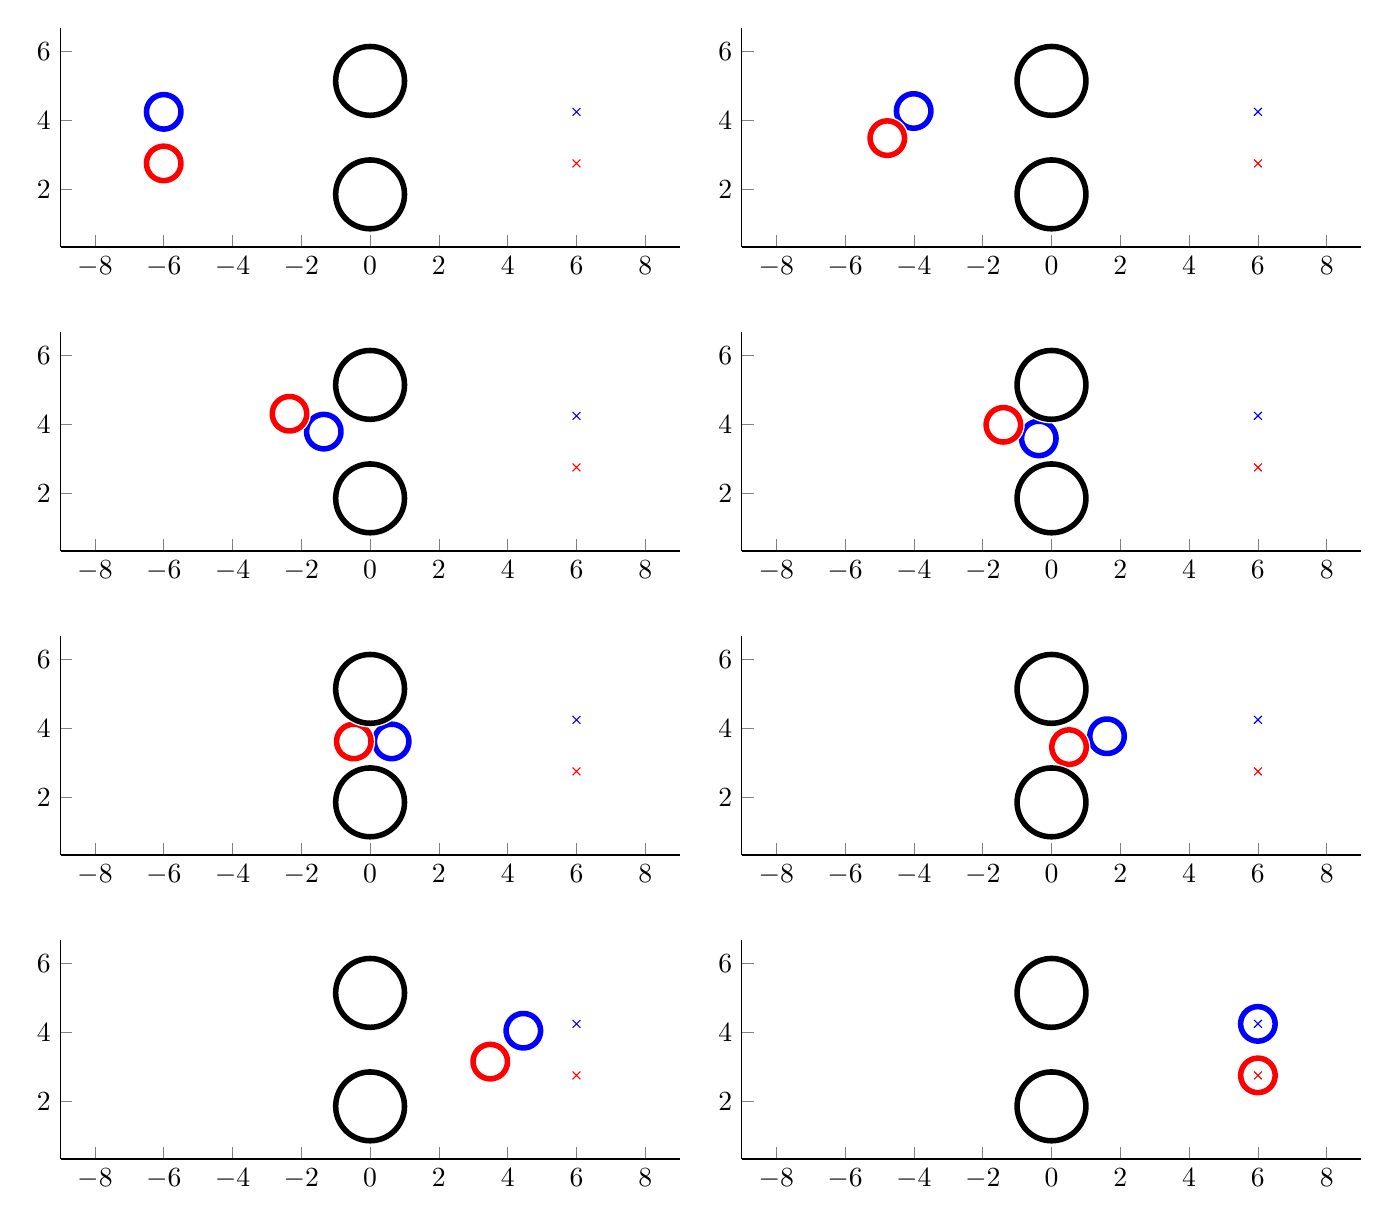
\begin{tikzpicture}

\begin{axis}[%
width=3.096in,
height=1.094in,
at={(2.593in,5.323in)},
scale only axis,
unbounded coords=jump,
xmin=-9,
xmax=9,
%xmajorgrids,
ymin=0.318379976997646,
ymax=6.68162002300235,
%ymajorgrids,
axis background/.style={fill=white},
axis x line*=bottom,
axis y line*=left
]
\addplot [color=blue,only marks,mark=x,mark options={solid},forget plot]
  table[row sep=crcr]{%
6	4.25\\
};
\addplot [color=red,only marks,mark=x,mark options={solid},forget plot]
  table[row sep=crcr]{%
6	2.75\\
};
\addplot [color=white,solid,line width=3.0pt,forget plot]
  table[row sep=crcr]{%
-5.5	4.25\\
-5.50030458649045	4.26744974835125\\
-5.50121797487009	4.28487823687206\\
-5.50273905231586	4.30226423163383\\
-5.50486596562921	4.31958655048003\\
-5.5075961234939	4.33682408883347\\
-5.5109261996331	4.35395584540888\\
-5.514852136862	4.37096094779983\\
-5.51936915203084	4.3878186779085\\
-5.52447174185242	4.40450849718747\\
-5.53015368960705	4.42101007166283\\
-5.53640807271661	4.43730329670796\\
-5.5432272711787	4.4533683215379\\
-5.55060297685042	4.46918557339454\\
-5.55852620357054	4.48473578139295\\
-5.56698729810778	4.5\\
-5.57597595192179	4.5149596321166\\
-5.58548121372248	4.52959645173537\\
-5.59549150281253	4.54389262614624\\
-5.60599462319664	4.55783073766283\\
-5.61697777844051	4.57139380484327\\
-5.6284275872613	4.58456530317943\\
-5.64033009983067	4.5973291852295\\
-5.6526708147705	4.60966990016933\\
-5.66543469682057	4.6215724127387\\
-5.67860619515673	4.63302222155949\\
-5.69216926233717	4.64400537680336\\
-5.70610737385376	4.65450849718747\\
-5.72040354826463	4.66451878627752\\
-5.7350403678834	4.67402404807821\\
-5.75	4.68301270189222\\
-5.76526421860705	4.69147379642946\\
-5.78081442660546	4.69939702314958\\
-5.7966316784621	4.7067727288213\\
-5.81269670329204	4.71359192728339\\
-5.82898992833717	4.71984631039295\\
-5.84549150281253	4.72552825814758\\
-5.8621813220915	4.73063084796916\\
-5.87903905220017	4.735147863138\\
-5.89604415459112	4.7390738003669\\
-5.91317591116653	4.7424038765061\\
-5.93041344951997	4.74513403437079\\
-5.94773576836617	4.74726094768414\\
-5.96512176312794	4.74878202512991\\
-5.98255025164875	4.74969541350955\\
-6	4.75\\
-6.01744974835125	4.74969541350955\\
-6.03487823687206	4.74878202512991\\
-6.05226423163383	4.74726094768414\\
-6.06958655048003	4.74513403437079\\
-6.08682408883347	4.7424038765061\\
-6.10395584540888	4.7390738003669\\
-6.12096094779983	4.735147863138\\
-6.1378186779085	4.73063084796916\\
-6.15450849718747	4.72552825814758\\
-6.17101007166283	4.71984631039295\\
-6.18730329670796	4.71359192728339\\
-6.2033683215379	4.7067727288213\\
-6.21918557339454	4.69939702314958\\
-6.23473578139295	4.69147379642946\\
-6.25	4.68301270189222\\
-6.2649596321166	4.67402404807821\\
-6.27959645173537	4.66451878627752\\
-6.29389262614624	4.65450849718747\\
-6.30783073766283	4.64400537680336\\
-6.32139380484327	4.63302222155949\\
-6.33456530317943	4.6215724127387\\
-6.3473291852295	4.60966990016933\\
-6.35966990016933	4.5973291852295\\
-6.3715724127387	4.58456530317943\\
-6.38302222155949	4.57139380484327\\
-6.39400537680336	4.55783073766283\\
-6.40450849718747	4.54389262614624\\
-6.41451878627752	4.52959645173537\\
-6.42402404807821	4.5149596321166\\
-6.43301270189222	4.5\\
-6.44147379642946	4.48473578139295\\
-6.44939702314958	4.46918557339454\\
-6.4567727288213	4.4533683215379\\
-6.46359192728339	4.43730329670796\\
-6.46984631039295	4.42101007166283\\
-6.47552825814758	4.40450849718747\\
-6.48063084796916	4.3878186779085\\
-6.485147863138	4.37096094779983\\
-6.4890738003669	4.35395584540888\\
-6.4924038765061	4.33682408883347\\
-6.49513403437079	4.31958655048003\\
-6.49726094768414	4.30226423163383\\
-6.49878202512991	4.28487823687206\\
-6.49969541350955	4.26744974835125\\
-6.5	4.25\\
-6.49969541350955	4.23255025164875\\
-6.49878202512991	4.21512176312794\\
-6.49726094768414	4.19773576836617\\
-6.49513403437079	4.18041344951997\\
-6.4924038765061	4.16317591116653\\
-6.4890738003669	4.14604415459112\\
-6.485147863138	4.12903905220017\\
-6.48063084796916	4.1121813220915\\
-6.47552825814758	4.09549150281253\\
-6.46984631039295	4.07898992833717\\
-6.46359192728339	4.06269670329204\\
-6.4567727288213	4.0466316784621\\
-6.44939702314958	4.03081442660546\\
-6.44147379642946	4.01526421860705\\
-6.43301270189222	4\\
-6.42402404807821	3.9850403678834\\
-6.41451878627752	3.97040354826463\\
-6.40450849718747	3.95610737385376\\
-6.39400537680336	3.94216926233717\\
-6.38302222155949	3.92860619515673\\
-6.3715724127387	3.91543469682057\\
-6.35966990016933	3.9026708147705\\
-6.3473291852295	3.89033009983067\\
-6.33456530317943	3.8784275872613\\
-6.32139380484327	3.86697777844051\\
-6.30783073766283	3.85599462319664\\
-6.29389262614624	3.84549150281253\\
-6.27959645173537	3.83548121372248\\
-6.2649596321166	3.82597595192179\\
-6.25	3.81698729810778\\
-6.23473578139295	3.80852620357054\\
-6.21918557339454	3.80060297685042\\
-6.2033683215379	3.7932272711787\\
-6.18730329670796	3.78640807271661\\
-6.17101007166283	3.78015368960705\\
-6.15450849718747	3.77447174185242\\
-6.1378186779085	3.76936915203084\\
-6.12096094779983	3.764852136862\\
-6.10395584540888	3.7609261996331\\
-6.08682408883347	3.7575961234939\\
-6.06958655048003	3.75486596562921\\
-6.05226423163383	3.75273905231586\\
-6.03487823687206	3.75121797487009\\
-6.01744974835125	3.75030458649045\\
-6	3.75\\
-5.98255025164875	3.75030458649045\\
-5.96512176312794	3.75121797487009\\
-5.94773576836617	3.75273905231586\\
-5.93041344951997	3.75486596562921\\
-5.91317591116653	3.7575961234939\\
-5.89604415459112	3.7609261996331\\
-5.87903905220017	3.764852136862\\
-5.8621813220915	3.76936915203084\\
-5.84549150281253	3.77447174185242\\
-5.82898992833717	3.78015368960705\\
-5.81269670329204	3.78640807271661\\
-5.7966316784621	3.7932272711787\\
-5.78081442660546	3.80060297685042\\
-5.76526421860705	3.80852620357054\\
-5.75	3.81698729810778\\
-5.7350403678834	3.82597595192179\\
-5.72040354826463	3.83548121372248\\
-5.70610737385376	3.84549150281253\\
-5.69216926233717	3.85599462319664\\
-5.67860619515673	3.86697777844051\\
-5.66543469682057	3.8784275872613\\
-5.6526708147705	3.89033009983067\\
-5.64033009983067	3.9026708147705\\
-5.6284275872613	3.91543469682057\\
-5.61697777844051	3.92860619515673\\
-5.60599462319664	3.94216926233717\\
-5.59549150281253	3.95610737385376\\
-5.58548121372248	3.97040354826463\\
-5.57597595192179	3.9850403678834\\
-5.56698729810778	4\\
-5.55852620357054	4.01526421860705\\
-5.55060297685042	4.03081442660546\\
-5.5432272711787	4.0466316784621\\
-5.53640807271661	4.06269670329204\\
-5.53015368960705	4.07898992833717\\
-5.52447174185242	4.09549150281253\\
-5.51936915203084	4.1121813220915\\
-5.514852136862	4.12903905220017\\
-5.5109261996331	4.14604415459112\\
-5.5075961234939	4.16317591116653\\
-5.50486596562921	4.18041344951997\\
-5.50273905231586	4.19773576836617\\
-5.50121797487009	4.21512176312794\\
-5.50030458649045	4.23255025164875\\
-5.5	4.25\\
nan	nan\\
};
\addplot [color=blue,solid,line width=2.0pt,forget plot]
  table[row sep=crcr]{%
-5.5	4.25\\
-5.50030458649045	4.26744974835125\\
-5.50121797487009	4.28487823687206\\
-5.50273905231586	4.30226423163383\\
-5.50486596562921	4.31958655048003\\
-5.5075961234939	4.33682408883347\\
-5.5109261996331	4.35395584540888\\
-5.514852136862	4.37096094779983\\
-5.51936915203084	4.3878186779085\\
-5.52447174185242	4.40450849718747\\
-5.53015368960705	4.42101007166283\\
-5.53640807271661	4.43730329670796\\
-5.5432272711787	4.4533683215379\\
-5.55060297685042	4.46918557339454\\
-5.55852620357054	4.48473578139295\\
-5.56698729810778	4.5\\
-5.57597595192179	4.5149596321166\\
-5.58548121372248	4.52959645173537\\
-5.59549150281253	4.54389262614624\\
-5.60599462319664	4.55783073766283\\
-5.61697777844051	4.57139380484327\\
-5.6284275872613	4.58456530317943\\
-5.64033009983067	4.5973291852295\\
-5.6526708147705	4.60966990016933\\
-5.66543469682057	4.6215724127387\\
-5.67860619515673	4.63302222155949\\
-5.69216926233717	4.64400537680336\\
-5.70610737385376	4.65450849718747\\
-5.72040354826463	4.66451878627752\\
-5.7350403678834	4.67402404807821\\
-5.75	4.68301270189222\\
-5.76526421860705	4.69147379642946\\
-5.78081442660546	4.69939702314958\\
-5.7966316784621	4.7067727288213\\
-5.81269670329204	4.71359192728339\\
-5.82898992833717	4.71984631039295\\
-5.84549150281253	4.72552825814758\\
-5.8621813220915	4.73063084796916\\
-5.87903905220017	4.735147863138\\
-5.89604415459112	4.7390738003669\\
-5.91317591116653	4.7424038765061\\
-5.93041344951997	4.74513403437079\\
-5.94773576836617	4.74726094768414\\
-5.96512176312794	4.74878202512991\\
-5.98255025164875	4.74969541350955\\
-6	4.75\\
-6.01744974835125	4.74969541350955\\
-6.03487823687206	4.74878202512991\\
-6.05226423163383	4.74726094768414\\
-6.06958655048003	4.74513403437079\\
-6.08682408883347	4.7424038765061\\
-6.10395584540888	4.7390738003669\\
-6.12096094779983	4.735147863138\\
-6.1378186779085	4.73063084796916\\
-6.15450849718747	4.72552825814758\\
-6.17101007166283	4.71984631039295\\
-6.18730329670796	4.71359192728339\\
-6.2033683215379	4.7067727288213\\
-6.21918557339454	4.69939702314958\\
-6.23473578139295	4.69147379642946\\
-6.25	4.68301270189222\\
-6.2649596321166	4.67402404807821\\
-6.27959645173537	4.66451878627752\\
-6.29389262614624	4.65450849718747\\
-6.30783073766283	4.64400537680336\\
-6.32139380484327	4.63302222155949\\
-6.33456530317943	4.6215724127387\\
-6.3473291852295	4.60966990016933\\
-6.35966990016933	4.5973291852295\\
-6.3715724127387	4.58456530317943\\
-6.38302222155949	4.57139380484327\\
-6.39400537680336	4.55783073766283\\
-6.40450849718747	4.54389262614624\\
-6.41451878627752	4.52959645173537\\
-6.42402404807821	4.5149596321166\\
-6.43301270189222	4.5\\
-6.44147379642946	4.48473578139295\\
-6.44939702314958	4.46918557339454\\
-6.4567727288213	4.4533683215379\\
-6.46359192728339	4.43730329670796\\
-6.46984631039295	4.42101007166283\\
-6.47552825814758	4.40450849718747\\
-6.48063084796916	4.3878186779085\\
-6.485147863138	4.37096094779983\\
-6.4890738003669	4.35395584540888\\
-6.4924038765061	4.33682408883347\\
-6.49513403437079	4.31958655048003\\
-6.49726094768414	4.30226423163383\\
-6.49878202512991	4.28487823687206\\
-6.49969541350955	4.26744974835125\\
-6.5	4.25\\
-6.49969541350955	4.23255025164875\\
-6.49878202512991	4.21512176312794\\
-6.49726094768414	4.19773576836617\\
-6.49513403437079	4.18041344951997\\
-6.4924038765061	4.16317591116653\\
-6.4890738003669	4.14604415459112\\
-6.485147863138	4.12903905220017\\
-6.48063084796916	4.1121813220915\\
-6.47552825814758	4.09549150281253\\
-6.46984631039295	4.07898992833717\\
-6.46359192728339	4.06269670329204\\
-6.4567727288213	4.0466316784621\\
-6.44939702314958	4.03081442660546\\
-6.44147379642946	4.01526421860705\\
-6.43301270189222	4\\
-6.42402404807821	3.9850403678834\\
-6.41451878627752	3.97040354826463\\
-6.40450849718747	3.95610737385376\\
-6.39400537680336	3.94216926233717\\
-6.38302222155949	3.92860619515673\\
-6.3715724127387	3.91543469682057\\
-6.35966990016933	3.9026708147705\\
-6.3473291852295	3.89033009983067\\
-6.33456530317943	3.8784275872613\\
-6.32139380484327	3.86697777844051\\
-6.30783073766283	3.85599462319664\\
-6.29389262614624	3.84549150281253\\
-6.27959645173537	3.83548121372248\\
-6.2649596321166	3.82597595192179\\
-6.25	3.81698729810778\\
-6.23473578139295	3.80852620357054\\
-6.21918557339454	3.80060297685042\\
-6.2033683215379	3.7932272711787\\
-6.18730329670796	3.78640807271661\\
-6.17101007166283	3.78015368960705\\
-6.15450849718747	3.77447174185242\\
-6.1378186779085	3.76936915203084\\
-6.12096094779983	3.764852136862\\
-6.10395584540888	3.7609261996331\\
-6.08682408883347	3.7575961234939\\
-6.06958655048003	3.75486596562921\\
-6.05226423163383	3.75273905231586\\
-6.03487823687206	3.75121797487009\\
-6.01744974835125	3.75030458649045\\
-6	3.75\\
-5.98255025164875	3.75030458649045\\
-5.96512176312794	3.75121797487009\\
-5.94773576836617	3.75273905231586\\
-5.93041344951997	3.75486596562921\\
-5.91317591116653	3.7575961234939\\
-5.89604415459112	3.7609261996331\\
-5.87903905220017	3.764852136862\\
-5.8621813220915	3.76936915203084\\
-5.84549150281253	3.77447174185242\\
-5.82898992833717	3.78015368960705\\
-5.81269670329204	3.78640807271661\\
-5.7966316784621	3.7932272711787\\
-5.78081442660546	3.80060297685042\\
-5.76526421860705	3.80852620357054\\
-5.75	3.81698729810778\\
-5.7350403678834	3.82597595192179\\
-5.72040354826463	3.83548121372248\\
-5.70610737385376	3.84549150281253\\
-5.69216926233717	3.85599462319664\\
-5.67860619515673	3.86697777844051\\
-5.66543469682057	3.8784275872613\\
-5.6526708147705	3.89033009983067\\
-5.64033009983067	3.9026708147705\\
-5.6284275872613	3.91543469682057\\
-5.61697777844051	3.92860619515673\\
-5.60599462319664	3.94216926233717\\
-5.59549150281253	3.95610737385376\\
-5.58548121372248	3.97040354826463\\
-5.57597595192179	3.9850403678834\\
-5.56698729810778	4\\
-5.55852620357054	4.01526421860705\\
-5.55060297685042	4.03081442660546\\
-5.5432272711787	4.0466316784621\\
-5.53640807271661	4.06269670329204\\
-5.53015368960705	4.07898992833717\\
-5.52447174185242	4.09549150281253\\
-5.51936915203084	4.1121813220915\\
-5.514852136862	4.12903905220017\\
-5.5109261996331	4.14604415459112\\
-5.5075961234939	4.16317591116653\\
-5.50486596562921	4.18041344951997\\
-5.50273905231586	4.19773576836617\\
-5.50121797487009	4.21512176312794\\
-5.50030458649045	4.23255025164875\\
-5.5	4.25\\
nan	nan\\
};
\addplot [color=white,solid,line width=3.0pt,forget plot]
  table[row sep=crcr]{%
-5.5	2.75\\
-5.50030458649045	2.76744974835125\\
-5.50121797487009	2.78487823687206\\
-5.50273905231586	2.80226423163383\\
-5.50486596562921	2.81958655048003\\
-5.5075961234939	2.83682408883347\\
-5.5109261996331	2.85395584540888\\
-5.514852136862	2.87096094779983\\
-5.51936915203084	2.8878186779085\\
-5.52447174185242	2.90450849718747\\
-5.53015368960705	2.92101007166283\\
-5.53640807271661	2.93730329670796\\
-5.5432272711787	2.9533683215379\\
-5.55060297685042	2.96918557339454\\
-5.55852620357054	2.98473578139295\\
-5.56698729810778	3\\
-5.57597595192179	3.0149596321166\\
-5.58548121372248	3.02959645173537\\
-5.59549150281253	3.04389262614624\\
-5.60599462319664	3.05783073766283\\
-5.61697777844051	3.07139380484327\\
-5.6284275872613	3.08456530317943\\
-5.64033009983067	3.0973291852295\\
-5.6526708147705	3.10966990016933\\
-5.66543469682057	3.1215724127387\\
-5.67860619515673	3.13302222155949\\
-5.69216926233717	3.14400537680336\\
-5.70610737385376	3.15450849718747\\
-5.72040354826463	3.16451878627752\\
-5.7350403678834	3.17402404807821\\
-5.75	3.18301270189222\\
-5.76526421860705	3.19147379642946\\
-5.78081442660546	3.19939702314958\\
-5.7966316784621	3.2067727288213\\
-5.81269670329204	3.21359192728339\\
-5.82898992833717	3.21984631039295\\
-5.84549150281253	3.22552825814758\\
-5.8621813220915	3.23063084796916\\
-5.87903905220017	3.235147863138\\
-5.89604415459112	3.2390738003669\\
-5.91317591116653	3.2424038765061\\
-5.93041344951997	3.24513403437079\\
-5.94773576836617	3.24726094768414\\
-5.96512176312794	3.24878202512991\\
-5.98255025164875	3.24969541350955\\
-6	3.25\\
-6.01744974835125	3.24969541350955\\
-6.03487823687206	3.24878202512991\\
-6.05226423163383	3.24726094768414\\
-6.06958655048003	3.24513403437079\\
-6.08682408883347	3.2424038765061\\
-6.10395584540888	3.2390738003669\\
-6.12096094779983	3.235147863138\\
-6.1378186779085	3.23063084796916\\
-6.15450849718747	3.22552825814758\\
-6.17101007166283	3.21984631039295\\
-6.18730329670796	3.21359192728339\\
-6.2033683215379	3.2067727288213\\
-6.21918557339454	3.19939702314958\\
-6.23473578139295	3.19147379642946\\
-6.25	3.18301270189222\\
-6.2649596321166	3.17402404807821\\
-6.27959645173537	3.16451878627752\\
-6.29389262614624	3.15450849718747\\
-6.30783073766283	3.14400537680336\\
-6.32139380484327	3.13302222155949\\
-6.33456530317943	3.1215724127387\\
-6.3473291852295	3.10966990016933\\
-6.35966990016933	3.0973291852295\\
-6.3715724127387	3.08456530317943\\
-6.38302222155949	3.07139380484327\\
-6.39400537680336	3.05783073766283\\
-6.40450849718747	3.04389262614624\\
-6.41451878627752	3.02959645173537\\
-6.42402404807821	3.0149596321166\\
-6.43301270189222	3\\
-6.44147379642946	2.98473578139295\\
-6.44939702314958	2.96918557339454\\
-6.4567727288213	2.9533683215379\\
-6.46359192728339	2.93730329670796\\
-6.46984631039295	2.92101007166283\\
-6.47552825814758	2.90450849718747\\
-6.48063084796916	2.8878186779085\\
-6.485147863138	2.87096094779983\\
-6.4890738003669	2.85395584540888\\
-6.4924038765061	2.83682408883347\\
-6.49513403437079	2.81958655048003\\
-6.49726094768414	2.80226423163383\\
-6.49878202512991	2.78487823687206\\
-6.49969541350955	2.76744974835125\\
-6.5	2.75\\
-6.49969541350955	2.73255025164875\\
-6.49878202512991	2.71512176312794\\
-6.49726094768414	2.69773576836617\\
-6.49513403437079	2.68041344951997\\
-6.4924038765061	2.66317591116653\\
-6.4890738003669	2.64604415459112\\
-6.485147863138	2.62903905220017\\
-6.48063084796916	2.6121813220915\\
-6.47552825814758	2.59549150281253\\
-6.46984631039295	2.57898992833717\\
-6.46359192728339	2.56269670329204\\
-6.4567727288213	2.5466316784621\\
-6.44939702314958	2.53081442660546\\
-6.44147379642946	2.51526421860705\\
-6.43301270189222	2.5\\
-6.42402404807821	2.4850403678834\\
-6.41451878627752	2.47040354826463\\
-6.40450849718747	2.45610737385376\\
-6.39400537680336	2.44216926233717\\
-6.38302222155949	2.42860619515673\\
-6.3715724127387	2.41543469682057\\
-6.35966990016933	2.4026708147705\\
-6.3473291852295	2.39033009983067\\
-6.33456530317943	2.3784275872613\\
-6.32139380484327	2.36697777844051\\
-6.30783073766283	2.35599462319664\\
-6.29389262614624	2.34549150281253\\
-6.27959645173537	2.33548121372248\\
-6.2649596321166	2.32597595192179\\
-6.25	2.31698729810778\\
-6.23473578139295	2.30852620357054\\
-6.21918557339454	2.30060297685042\\
-6.2033683215379	2.2932272711787\\
-6.18730329670796	2.28640807271661\\
-6.17101007166283	2.28015368960705\\
-6.15450849718747	2.27447174185242\\
-6.1378186779085	2.26936915203084\\
-6.12096094779983	2.264852136862\\
-6.10395584540888	2.2609261996331\\
-6.08682408883347	2.2575961234939\\
-6.06958655048003	2.25486596562921\\
-6.05226423163383	2.25273905231586\\
-6.03487823687206	2.25121797487009\\
-6.01744974835125	2.25030458649045\\
-6	2.25\\
-5.98255025164875	2.25030458649045\\
-5.96512176312794	2.25121797487009\\
-5.94773576836617	2.25273905231586\\
-5.93041344951997	2.25486596562921\\
-5.91317591116653	2.2575961234939\\
-5.89604415459112	2.2609261996331\\
-5.87903905220017	2.264852136862\\
-5.8621813220915	2.26936915203084\\
-5.84549150281253	2.27447174185242\\
-5.82898992833717	2.28015368960705\\
-5.81269670329204	2.28640807271661\\
-5.7966316784621	2.2932272711787\\
-5.78081442660546	2.30060297685042\\
-5.76526421860705	2.30852620357054\\
-5.75	2.31698729810778\\
-5.7350403678834	2.32597595192179\\
-5.72040354826463	2.33548121372248\\
-5.70610737385376	2.34549150281253\\
-5.69216926233717	2.35599462319664\\
-5.67860619515673	2.36697777844051\\
-5.66543469682057	2.3784275872613\\
-5.6526708147705	2.39033009983067\\
-5.64033009983067	2.4026708147705\\
-5.6284275872613	2.41543469682057\\
-5.61697777844051	2.42860619515673\\
-5.60599462319664	2.44216926233717\\
-5.59549150281253	2.45610737385376\\
-5.58548121372248	2.47040354826463\\
-5.57597595192179	2.4850403678834\\
-5.56698729810778	2.5\\
-5.55852620357054	2.51526421860705\\
-5.55060297685042	2.53081442660546\\
-5.5432272711787	2.5466316784621\\
-5.53640807271661	2.56269670329204\\
-5.53015368960705	2.57898992833717\\
-5.52447174185242	2.59549150281253\\
-5.51936915203084	2.6121813220915\\
-5.514852136862	2.62903905220017\\
-5.5109261996331	2.64604415459112\\
-5.5075961234939	2.66317591116653\\
-5.50486596562921	2.68041344951997\\
-5.50273905231586	2.69773576836617\\
-5.50121797487009	2.71512176312794\\
-5.50030458649045	2.73255025164875\\
-5.5	2.75\\
nan	nan\\
};
\addplot [color=red,solid,line width=2.0pt,forget plot]
  table[row sep=crcr]{%
-5.5	2.75\\
-5.50030458649045	2.76744974835125\\
-5.50121797487009	2.78487823687206\\
-5.50273905231586	2.80226423163383\\
-5.50486596562921	2.81958655048003\\
-5.5075961234939	2.83682408883347\\
-5.5109261996331	2.85395584540888\\
-5.514852136862	2.87096094779983\\
-5.51936915203084	2.8878186779085\\
-5.52447174185242	2.90450849718747\\
-5.53015368960705	2.92101007166283\\
-5.53640807271661	2.93730329670796\\
-5.5432272711787	2.9533683215379\\
-5.55060297685042	2.96918557339454\\
-5.55852620357054	2.98473578139295\\
-5.56698729810778	3\\
-5.57597595192179	3.0149596321166\\
-5.58548121372248	3.02959645173537\\
-5.59549150281253	3.04389262614624\\
-5.60599462319664	3.05783073766283\\
-5.61697777844051	3.07139380484327\\
-5.6284275872613	3.08456530317943\\
-5.64033009983067	3.0973291852295\\
-5.6526708147705	3.10966990016933\\
-5.66543469682057	3.1215724127387\\
-5.67860619515673	3.13302222155949\\
-5.69216926233717	3.14400537680336\\
-5.70610737385376	3.15450849718747\\
-5.72040354826463	3.16451878627752\\
-5.7350403678834	3.17402404807821\\
-5.75	3.18301270189222\\
-5.76526421860705	3.19147379642946\\
-5.78081442660546	3.19939702314958\\
-5.7966316784621	3.2067727288213\\
-5.81269670329204	3.21359192728339\\
-5.82898992833717	3.21984631039295\\
-5.84549150281253	3.22552825814758\\
-5.8621813220915	3.23063084796916\\
-5.87903905220017	3.235147863138\\
-5.89604415459112	3.2390738003669\\
-5.91317591116653	3.2424038765061\\
-5.93041344951997	3.24513403437079\\
-5.94773576836617	3.24726094768414\\
-5.96512176312794	3.24878202512991\\
-5.98255025164875	3.24969541350955\\
-6	3.25\\
-6.01744974835125	3.24969541350955\\
-6.03487823687206	3.24878202512991\\
-6.05226423163383	3.24726094768414\\
-6.06958655048003	3.24513403437079\\
-6.08682408883347	3.2424038765061\\
-6.10395584540888	3.2390738003669\\
-6.12096094779983	3.235147863138\\
-6.1378186779085	3.23063084796916\\
-6.15450849718747	3.22552825814758\\
-6.17101007166283	3.21984631039295\\
-6.18730329670796	3.21359192728339\\
-6.2033683215379	3.2067727288213\\
-6.21918557339454	3.19939702314958\\
-6.23473578139295	3.19147379642946\\
-6.25	3.18301270189222\\
-6.2649596321166	3.17402404807821\\
-6.27959645173537	3.16451878627752\\
-6.29389262614624	3.15450849718747\\
-6.30783073766283	3.14400537680336\\
-6.32139380484327	3.13302222155949\\
-6.33456530317943	3.1215724127387\\
-6.3473291852295	3.10966990016933\\
-6.35966990016933	3.0973291852295\\
-6.3715724127387	3.08456530317943\\
-6.38302222155949	3.07139380484327\\
-6.39400537680336	3.05783073766283\\
-6.40450849718747	3.04389262614624\\
-6.41451878627752	3.02959645173537\\
-6.42402404807821	3.0149596321166\\
-6.43301270189222	3\\
-6.44147379642946	2.98473578139295\\
-6.44939702314958	2.96918557339454\\
-6.4567727288213	2.9533683215379\\
-6.46359192728339	2.93730329670796\\
-6.46984631039295	2.92101007166283\\
-6.47552825814758	2.90450849718747\\
-6.48063084796916	2.8878186779085\\
-6.485147863138	2.87096094779983\\
-6.4890738003669	2.85395584540888\\
-6.4924038765061	2.83682408883347\\
-6.49513403437079	2.81958655048003\\
-6.49726094768414	2.80226423163383\\
-6.49878202512991	2.78487823687206\\
-6.49969541350955	2.76744974835125\\
-6.5	2.75\\
-6.49969541350955	2.73255025164875\\
-6.49878202512991	2.71512176312794\\
-6.49726094768414	2.69773576836617\\
-6.49513403437079	2.68041344951997\\
-6.4924038765061	2.66317591116653\\
-6.4890738003669	2.64604415459112\\
-6.485147863138	2.62903905220017\\
-6.48063084796916	2.6121813220915\\
-6.47552825814758	2.59549150281253\\
-6.46984631039295	2.57898992833717\\
-6.46359192728339	2.56269670329204\\
-6.4567727288213	2.5466316784621\\
-6.44939702314958	2.53081442660546\\
-6.44147379642946	2.51526421860705\\
-6.43301270189222	2.5\\
-6.42402404807821	2.4850403678834\\
-6.41451878627752	2.47040354826463\\
-6.40450849718747	2.45610737385376\\
-6.39400537680336	2.44216926233717\\
-6.38302222155949	2.42860619515673\\
-6.3715724127387	2.41543469682057\\
-6.35966990016933	2.4026708147705\\
-6.3473291852295	2.39033009983067\\
-6.33456530317943	2.3784275872613\\
-6.32139380484327	2.36697777844051\\
-6.30783073766283	2.35599462319664\\
-6.29389262614624	2.34549150281253\\
-6.27959645173537	2.33548121372248\\
-6.2649596321166	2.32597595192179\\
-6.25	2.31698729810778\\
-6.23473578139295	2.30852620357054\\
-6.21918557339454	2.30060297685042\\
-6.2033683215379	2.2932272711787\\
-6.18730329670796	2.28640807271661\\
-6.17101007166283	2.28015368960705\\
-6.15450849718747	2.27447174185242\\
-6.1378186779085	2.26936915203084\\
-6.12096094779983	2.264852136862\\
-6.10395584540888	2.2609261996331\\
-6.08682408883347	2.2575961234939\\
-6.06958655048003	2.25486596562921\\
-6.05226423163383	2.25273905231586\\
-6.03487823687206	2.25121797487009\\
-6.01744974835125	2.25030458649045\\
-6	2.25\\
-5.98255025164875	2.25030458649045\\
-5.96512176312794	2.25121797487009\\
-5.94773576836617	2.25273905231586\\
-5.93041344951997	2.25486596562921\\
-5.91317591116653	2.2575961234939\\
-5.89604415459112	2.2609261996331\\
-5.87903905220017	2.264852136862\\
-5.8621813220915	2.26936915203084\\
-5.84549150281253	2.27447174185242\\
-5.82898992833717	2.28015368960705\\
-5.81269670329204	2.28640807271661\\
-5.7966316784621	2.2932272711787\\
-5.78081442660546	2.30060297685042\\
-5.76526421860705	2.30852620357054\\
-5.75	2.31698729810778\\
-5.7350403678834	2.32597595192179\\
-5.72040354826463	2.33548121372248\\
-5.70610737385376	2.34549150281253\\
-5.69216926233717	2.35599462319664\\
-5.67860619515673	2.36697777844051\\
-5.66543469682057	2.3784275872613\\
-5.6526708147705	2.39033009983067\\
-5.64033009983067	2.4026708147705\\
-5.6284275872613	2.41543469682057\\
-5.61697777844051	2.42860619515673\\
-5.60599462319664	2.44216926233717\\
-5.59549150281253	2.45610737385376\\
-5.58548121372248	2.47040354826463\\
-5.57597595192179	2.4850403678834\\
-5.56698729810778	2.5\\
-5.55852620357054	2.51526421860705\\
-5.55060297685042	2.53081442660546\\
-5.5432272711787	2.5466316784621\\
-5.53640807271661	2.56269670329204\\
-5.53015368960705	2.57898992833717\\
-5.52447174185242	2.59549150281253\\
-5.51936915203084	2.6121813220915\\
-5.514852136862	2.62903905220017\\
-5.5109261996331	2.64604415459112\\
-5.5075961234939	2.66317591116653\\
-5.50486596562921	2.68041344951997\\
-5.50273905231586	2.69773576836617\\
-5.50121797487009	2.71512176312794\\
-5.50030458649045	2.73255025164875\\
-5.5	2.75\\
nan	nan\\
};
\addplot [color=white,solid,line width=3.0pt,forget plot]
  table[row sep=crcr]{%
1	1.85\\
0.999390827019096	1.8848994967025\\
0.997564050259824	1.91975647374413\\
0.994521895368273	1.95452846326765\\
0.99026806874157	1.98917310096007\\
0.984807753012208	2.02364817766693\\
0.978147600733806	2.05791169081776\\
0.970295726275996	2.09192189559967\\
0.961261695938319	2.125637355817\\
0.951056516295154	2.15901699437495\\
0.939692620785908	2.19202014332567\\
0.927183854566787	2.22460659341591\\
0.913545457642601	2.2567366430758\\
0.898794046299167	2.28837114678908\\
0.882947592858927	2.31947156278589\\
0.866025403784439	2.35\\
0.848048096156426	2.37991926423321\\
0.829037572555042	2.40919290347075\\
0.809016994374947	2.43778525229247\\
0.788010753606722	2.46566147532566\\
0.766044443118978	2.49278760968654\\
0.743144825477394	2.51913060635886\\
0.719339800338651	2.544658370459\\
0.694658370458997	2.56933980033865\\
0.669130606358858	2.59314482547739\\
0.642787609686539	2.61604444311898\\
0.615661475325658	2.63801075360672\\
0.587785252292473	2.65901699437495\\
0.559192903470747	2.67903757255504\\
0.529919264233205	2.69804809615643\\
0.5	2.71602540378444\\
0.469471562785891	2.73294759285893\\
0.438371146789077	2.74879404629917\\
0.4067366430758	2.7635454576426\\
0.374606593415912	2.77718385456679\\
0.342020143325669	2.78969262078591\\
0.309016994374947	2.80105651629515\\
0.275637355816999	2.81126169593832\\
0.241921895599668	2.820295726276\\
0.207911690817759	2.82814760073381\\
0.17364817766693	2.83480775301221\\
0.139173100960066	2.84026806874157\\
0.104528463267653	2.84452189536827\\
0.0697564737441255	2.84756405025982\\
0.0348994967025011	2.8493908270191\\
6.12323399573677e-17	2.85\\
-0.0348994967025007	2.8493908270191\\
-0.0697564737441253	2.84756405025982\\
-0.104528463267653	2.84452189536827\\
-0.139173100960065	2.84026806874157\\
-0.17364817766693	2.83480775301221\\
-0.207911690817759	2.82814760073381\\
-0.241921895599668	2.820295726276\\
-0.275637355816999	2.81126169593832\\
-0.309016994374947	2.80105651629515\\
-0.342020143325669	2.78969262078591\\
-0.374606593415912	2.77718385456679\\
-0.4067366430758	2.7635454576426\\
-0.438371146789078	2.74879404629917\\
-0.469471562785891	2.73294759285893\\
-0.5	2.71602540378444\\
-0.529919264233205	2.69804809615643\\
-0.559192903470747	2.67903757255504\\
-0.587785252292473	2.65901699437495\\
-0.615661475325658	2.63801075360672\\
-0.642787609686539	2.61604444311898\\
-0.669130606358858	2.59314482547739\\
-0.694658370458997	2.56933980033865\\
-0.719339800338651	2.544658370459\\
-0.743144825477394	2.51913060635886\\
-0.766044443118978	2.49278760968654\\
-0.788010753606722	2.46566147532566\\
-0.809016994374947	2.43778525229247\\
-0.829037572555042	2.40919290347075\\
-0.848048096156426	2.37991926423321\\
-0.866025403784439	2.35\\
-0.882947592858927	2.31947156278589\\
-0.898794046299167	2.28837114678908\\
-0.913545457642601	2.2567366430758\\
-0.927183854566787	2.22460659341591\\
-0.939692620785908	2.19202014332567\\
-0.951056516295154	2.15901699437495\\
-0.961261695938319	2.125637355817\\
-0.970295726275996	2.09192189559967\\
-0.978147600733806	2.05791169081776\\
-0.984807753012208	2.02364817766693\\
-0.99026806874157	1.98917310096007\\
-0.994521895368273	1.95452846326765\\
-0.997564050259824	1.91975647374413\\
-0.999390827019096	1.8848994967025\\
-1	1.85\\
-0.999390827019096	1.8151005032975\\
-0.997564050259824	1.78024352625588\\
-0.994521895368273	1.74547153673235\\
-0.99026806874157	1.71082689903993\\
-0.984807753012208	1.67635182233307\\
-0.978147600733806	1.64208830918224\\
-0.970295726275997	1.60807810440033\\
-0.961261695938319	1.574362644183\\
-0.951056516295154	1.54098300562505\\
-0.939692620785908	1.50797985667433\\
-0.927183854566787	1.47539340658409\\
-0.913545457642601	1.4432633569242\\
-0.898794046299167	1.41162885321092\\
-0.882947592858927	1.38052843721411\\
-0.866025403784439	1.35\\
-0.848048096156426	1.3200807357668\\
-0.829037572555042	1.29080709652925\\
-0.809016994374947	1.26221474770753\\
-0.788010753606722	1.23433852467434\\
-0.766044443118978	1.20721239031346\\
-0.743144825477394	1.18086939364114\\
-0.719339800338651	1.155341629541\\
-0.694658370458997	1.13066019966135\\
-0.669130606358858	1.10685517452261\\
-0.642787609686539	1.08395555688102\\
-0.615661475325658	1.06198924639328\\
-0.587785252292473	1.04098300562505\\
-0.559192903470747	1.02096242744496\\
-0.529919264233205	1.00195190384357\\
-0.5	0.983974596215562\\
-0.469471562785891	0.967052407141073\\
-0.438371146789078	0.951205953700833\\
-0.4067366430758	0.936454542357399\\
-0.374606593415912	0.922816145433213\\
-0.342020143325669	0.910307379214092\\
-0.309016994374948	0.898943483704847\\
-0.275637355816999	0.888738304061681\\
-0.241921895599668	0.879704273724004\\
-0.20791169081776	0.871852399266195\\
-0.17364817766693	0.865192246987792\\
-0.139173100960065	0.85973193125843\\
-0.104528463267653	0.855478104631727\\
-0.0697564737441256	0.852435949740176\\
-0.0348994967025016	0.850609172980904\\
-1.83697019872103e-16	0.85\\
0.0348994967025013	0.850609172980904\\
0.0697564737441252	0.852435949740176\\
0.104528463267653	0.855478104631727\\
0.139173100960065	0.85973193125843\\
0.17364817766693	0.865192246987792\\
0.207911690817759	0.871852399266194\\
0.241921895599667	0.879704273724004\\
0.275637355816999	0.888738304061681\\
0.309016994374947	0.898943483704846\\
0.342020143325668	0.910307379214092\\
0.374606593415912	0.922816145433213\\
0.406736643075801	0.936454542357399\\
0.438371146789077	0.951205953700833\\
0.46947156278589	0.967052407141073\\
0.5	0.983974596215561\\
0.529919264233205	1.00195190384357\\
0.559192903470746	1.02096242744496\\
0.587785252292473	1.04098300562505\\
0.615661475325659	1.06198924639328\\
0.642787609686539	1.08395555688102\\
0.669130606358858	1.10685517452261\\
0.694658370458997	1.13066019966135\\
0.719339800338651	1.155341629541\\
0.743144825477394	1.18086939364114\\
0.766044443118978	1.20721239031346\\
0.788010753606722	1.23433852467434\\
0.809016994374947	1.26221474770753\\
0.829037572555041	1.29080709652925\\
0.848048096156425	1.32008073576679\\
0.866025403784438	1.35\\
0.882947592858927	1.38052843721411\\
0.898794046299167	1.41162885321092\\
0.913545457642601	1.4432633569242\\
0.927183854566787	1.47539340658409\\
0.939692620785908	1.50797985667433\\
0.951056516295154	1.54098300562505\\
0.961261695938319	1.574362644183\\
0.970295726275996	1.60807810440033\\
0.978147600733806	1.64208830918224\\
0.984807753012208	1.67635182233307\\
0.99026806874157	1.71082689903993\\
0.994521895368273	1.74547153673235\\
0.997564050259824	1.78024352625588\\
0.999390827019096	1.8151005032975\\
1	1.85\\
nan	nan\\
};
\addplot [color=black,solid,line width=2.0pt,forget plot]
  table[row sep=crcr]{%
1	1.85\\
0.999390827019096	1.8848994967025\\
0.997564050259824	1.91975647374413\\
0.994521895368273	1.95452846326765\\
0.99026806874157	1.98917310096007\\
0.984807753012208	2.02364817766693\\
0.978147600733806	2.05791169081776\\
0.970295726275996	2.09192189559967\\
0.961261695938319	2.125637355817\\
0.951056516295154	2.15901699437495\\
0.939692620785908	2.19202014332567\\
0.927183854566787	2.22460659341591\\
0.913545457642601	2.2567366430758\\
0.898794046299167	2.28837114678908\\
0.882947592858927	2.31947156278589\\
0.866025403784439	2.35\\
0.848048096156426	2.37991926423321\\
0.829037572555042	2.40919290347075\\
0.809016994374947	2.43778525229247\\
0.788010753606722	2.46566147532566\\
0.766044443118978	2.49278760968654\\
0.743144825477394	2.51913060635886\\
0.719339800338651	2.544658370459\\
0.694658370458997	2.56933980033865\\
0.669130606358858	2.59314482547739\\
0.642787609686539	2.61604444311898\\
0.615661475325658	2.63801075360672\\
0.587785252292473	2.65901699437495\\
0.559192903470747	2.67903757255504\\
0.529919264233205	2.69804809615643\\
0.5	2.71602540378444\\
0.469471562785891	2.73294759285893\\
0.438371146789077	2.74879404629917\\
0.4067366430758	2.7635454576426\\
0.374606593415912	2.77718385456679\\
0.342020143325669	2.78969262078591\\
0.309016994374947	2.80105651629515\\
0.275637355816999	2.81126169593832\\
0.241921895599668	2.820295726276\\
0.207911690817759	2.82814760073381\\
0.17364817766693	2.83480775301221\\
0.139173100960066	2.84026806874157\\
0.104528463267653	2.84452189536827\\
0.0697564737441255	2.84756405025982\\
0.0348994967025011	2.8493908270191\\
6.12323399573677e-17	2.85\\
-0.0348994967025007	2.8493908270191\\
-0.0697564737441253	2.84756405025982\\
-0.104528463267653	2.84452189536827\\
-0.139173100960065	2.84026806874157\\
-0.17364817766693	2.83480775301221\\
-0.207911690817759	2.82814760073381\\
-0.241921895599668	2.820295726276\\
-0.275637355816999	2.81126169593832\\
-0.309016994374947	2.80105651629515\\
-0.342020143325669	2.78969262078591\\
-0.374606593415912	2.77718385456679\\
-0.4067366430758	2.7635454576426\\
-0.438371146789078	2.74879404629917\\
-0.469471562785891	2.73294759285893\\
-0.5	2.71602540378444\\
-0.529919264233205	2.69804809615643\\
-0.559192903470747	2.67903757255504\\
-0.587785252292473	2.65901699437495\\
-0.615661475325658	2.63801075360672\\
-0.642787609686539	2.61604444311898\\
-0.669130606358858	2.59314482547739\\
-0.694658370458997	2.56933980033865\\
-0.719339800338651	2.544658370459\\
-0.743144825477394	2.51913060635886\\
-0.766044443118978	2.49278760968654\\
-0.788010753606722	2.46566147532566\\
-0.809016994374947	2.43778525229247\\
-0.829037572555042	2.40919290347075\\
-0.848048096156426	2.37991926423321\\
-0.866025403784439	2.35\\
-0.882947592858927	2.31947156278589\\
-0.898794046299167	2.28837114678908\\
-0.913545457642601	2.2567366430758\\
-0.927183854566787	2.22460659341591\\
-0.939692620785908	2.19202014332567\\
-0.951056516295154	2.15901699437495\\
-0.961261695938319	2.125637355817\\
-0.970295726275996	2.09192189559967\\
-0.978147600733806	2.05791169081776\\
-0.984807753012208	2.02364817766693\\
-0.99026806874157	1.98917310096007\\
-0.994521895368273	1.95452846326765\\
-0.997564050259824	1.91975647374413\\
-0.999390827019096	1.8848994967025\\
-1	1.85\\
-0.999390827019096	1.8151005032975\\
-0.997564050259824	1.78024352625588\\
-0.994521895368273	1.74547153673235\\
-0.99026806874157	1.71082689903993\\
-0.984807753012208	1.67635182233307\\
-0.978147600733806	1.64208830918224\\
-0.970295726275997	1.60807810440033\\
-0.961261695938319	1.574362644183\\
-0.951056516295154	1.54098300562505\\
-0.939692620785908	1.50797985667433\\
-0.927183854566787	1.47539340658409\\
-0.913545457642601	1.4432633569242\\
-0.898794046299167	1.41162885321092\\
-0.882947592858927	1.38052843721411\\
-0.866025403784439	1.35\\
-0.848048096156426	1.3200807357668\\
-0.829037572555042	1.29080709652925\\
-0.809016994374947	1.26221474770753\\
-0.788010753606722	1.23433852467434\\
-0.766044443118978	1.20721239031346\\
-0.743144825477394	1.18086939364114\\
-0.719339800338651	1.155341629541\\
-0.694658370458997	1.13066019966135\\
-0.669130606358858	1.10685517452261\\
-0.642787609686539	1.08395555688102\\
-0.615661475325658	1.06198924639328\\
-0.587785252292473	1.04098300562505\\
-0.559192903470747	1.02096242744496\\
-0.529919264233205	1.00195190384357\\
-0.5	0.983974596215562\\
-0.469471562785891	0.967052407141073\\
-0.438371146789078	0.951205953700833\\
-0.4067366430758	0.936454542357399\\
-0.374606593415912	0.922816145433213\\
-0.342020143325669	0.910307379214092\\
-0.309016994374948	0.898943483704847\\
-0.275637355816999	0.888738304061681\\
-0.241921895599668	0.879704273724004\\
-0.20791169081776	0.871852399266195\\
-0.17364817766693	0.865192246987792\\
-0.139173100960065	0.85973193125843\\
-0.104528463267653	0.855478104631727\\
-0.0697564737441256	0.852435949740176\\
-0.0348994967025016	0.850609172980904\\
-1.83697019872103e-16	0.85\\
0.0348994967025013	0.850609172980904\\
0.0697564737441252	0.852435949740176\\
0.104528463267653	0.855478104631727\\
0.139173100960065	0.85973193125843\\
0.17364817766693	0.865192246987792\\
0.207911690817759	0.871852399266194\\
0.241921895599667	0.879704273724004\\
0.275637355816999	0.888738304061681\\
0.309016994374947	0.898943483704846\\
0.342020143325668	0.910307379214092\\
0.374606593415912	0.922816145433213\\
0.406736643075801	0.936454542357399\\
0.438371146789077	0.951205953700833\\
0.46947156278589	0.967052407141073\\
0.5	0.983974596215561\\
0.529919264233205	1.00195190384357\\
0.559192903470746	1.02096242744496\\
0.587785252292473	1.04098300562505\\
0.615661475325659	1.06198924639328\\
0.642787609686539	1.08395555688102\\
0.669130606358858	1.10685517452261\\
0.694658370458997	1.13066019966135\\
0.719339800338651	1.155341629541\\
0.743144825477394	1.18086939364114\\
0.766044443118978	1.20721239031346\\
0.788010753606722	1.23433852467434\\
0.809016994374947	1.26221474770753\\
0.829037572555041	1.29080709652925\\
0.848048096156425	1.32008073576679\\
0.866025403784438	1.35\\
0.882947592858927	1.38052843721411\\
0.898794046299167	1.41162885321092\\
0.913545457642601	1.4432633569242\\
0.927183854566787	1.47539340658409\\
0.939692620785908	1.50797985667433\\
0.951056516295154	1.54098300562505\\
0.961261695938319	1.574362644183\\
0.970295726275996	1.60807810440033\\
0.978147600733806	1.64208830918224\\
0.984807753012208	1.67635182233307\\
0.99026806874157	1.71082689903993\\
0.994521895368273	1.74547153673235\\
0.997564050259824	1.78024352625588\\
0.999390827019096	1.8151005032975\\
1	1.85\\
nan	nan\\
};
\addplot [color=white,solid,line width=3.0pt,forget plot]
  table[row sep=crcr]{%
1	5.15\\
0.999390827019096	5.1848994967025\\
0.997564050259824	5.21975647374413\\
0.994521895368273	5.25452846326765\\
0.99026806874157	5.28917310096007\\
0.984807753012208	5.32364817766693\\
0.978147600733806	5.35791169081776\\
0.970295726275996	5.39192189559967\\
0.961261695938319	5.425637355817\\
0.951056516295154	5.45901699437495\\
0.939692620785908	5.49202014332567\\
0.927183854566787	5.52460659341591\\
0.913545457642601	5.5567366430758\\
0.898794046299167	5.58837114678908\\
0.882947592858927	5.61947156278589\\
0.866025403784439	5.65\\
0.848048096156426	5.67991926423321\\
0.829037572555042	5.70919290347075\\
0.809016994374947	5.73778525229247\\
0.788010753606722	5.76566147532566\\
0.766044443118978	5.79278760968654\\
0.743144825477394	5.81913060635886\\
0.719339800338651	5.844658370459\\
0.694658370458997	5.86933980033865\\
0.669130606358858	5.89314482547739\\
0.642787609686539	5.91604444311898\\
0.615661475325658	5.93801075360672\\
0.587785252292473	5.95901699437495\\
0.559192903470747	5.97903757255504\\
0.529919264233205	5.99804809615643\\
0.5	6.01602540378444\\
0.469471562785891	6.03294759285893\\
0.438371146789077	6.04879404629917\\
0.4067366430758	6.0635454576426\\
0.374606593415912	6.07718385456679\\
0.342020143325669	6.08969262078591\\
0.309016994374947	6.10105651629515\\
0.275637355816999	6.11126169593832\\
0.241921895599668	6.120295726276\\
0.207911690817759	6.12814760073381\\
0.17364817766693	6.13480775301221\\
0.139173100960066	6.14026806874157\\
0.104528463267653	6.14452189536827\\
0.0697564737441255	6.14756405025982\\
0.0348994967025011	6.1493908270191\\
6.12323399573677e-17	6.15\\
-0.0348994967025007	6.1493908270191\\
-0.0697564737441253	6.14756405025982\\
-0.104528463267653	6.14452189536827\\
-0.139173100960065	6.14026806874157\\
-0.17364817766693	6.13480775301221\\
-0.207911690817759	6.12814760073381\\
-0.241921895599668	6.120295726276\\
-0.275637355816999	6.11126169593832\\
-0.309016994374947	6.10105651629515\\
-0.342020143325669	6.08969262078591\\
-0.374606593415912	6.07718385456679\\
-0.4067366430758	6.0635454576426\\
-0.438371146789078	6.04879404629917\\
-0.469471562785891	6.03294759285893\\
-0.5	6.01602540378444\\
-0.529919264233205	5.99804809615643\\
-0.559192903470747	5.97903757255504\\
-0.587785252292473	5.95901699437495\\
-0.615661475325658	5.93801075360672\\
-0.642787609686539	5.91604444311898\\
-0.669130606358858	5.89314482547739\\
-0.694658370458997	5.86933980033865\\
-0.719339800338651	5.844658370459\\
-0.743144825477394	5.81913060635886\\
-0.766044443118978	5.79278760968654\\
-0.788010753606722	5.76566147532566\\
-0.809016994374947	5.73778525229247\\
-0.829037572555042	5.70919290347075\\
-0.848048096156426	5.67991926423321\\
-0.866025403784439	5.65\\
-0.882947592858927	5.61947156278589\\
-0.898794046299167	5.58837114678908\\
-0.913545457642601	5.5567366430758\\
-0.927183854566787	5.52460659341591\\
-0.939692620785908	5.49202014332567\\
-0.951056516295154	5.45901699437495\\
-0.961261695938319	5.425637355817\\
-0.970295726275996	5.39192189559967\\
-0.978147600733806	5.35791169081776\\
-0.984807753012208	5.32364817766693\\
-0.99026806874157	5.28917310096007\\
-0.994521895368273	5.25452846326765\\
-0.997564050259824	5.21975647374413\\
-0.999390827019096	5.1848994967025\\
-1	5.15\\
-0.999390827019096	5.1151005032975\\
-0.997564050259824	5.08024352625588\\
-0.994521895368273	5.04547153673235\\
-0.99026806874157	5.01082689903993\\
-0.984807753012208	4.97635182233307\\
-0.978147600733806	4.94208830918224\\
-0.970295726275997	4.90807810440033\\
-0.961261695938319	4.874362644183\\
-0.951056516295154	4.84098300562505\\
-0.939692620785908	4.80797985667433\\
-0.927183854566787	4.77539340658409\\
-0.913545457642601	4.7432633569242\\
-0.898794046299167	4.71162885321092\\
-0.882947592858927	4.68052843721411\\
-0.866025403784439	4.65\\
-0.848048096156426	4.6200807357668\\
-0.829037572555042	4.59080709652925\\
-0.809016994374947	4.56221474770753\\
-0.788010753606722	4.53433852467434\\
-0.766044443118978	4.50721239031346\\
-0.743144825477394	4.48086939364114\\
-0.719339800338651	4.455341629541\\
-0.694658370458997	4.43066019966135\\
-0.669130606358858	4.40685517452261\\
-0.642787609686539	4.38395555688102\\
-0.615661475325658	4.36198924639328\\
-0.587785252292473	4.34098300562505\\
-0.559192903470747	4.32096242744496\\
-0.529919264233205	4.30195190384357\\
-0.5	4.28397459621556\\
-0.469471562785891	4.26705240714107\\
-0.438371146789078	4.25120595370083\\
-0.4067366430758	4.2364545423574\\
-0.374606593415912	4.22281614543321\\
-0.342020143325669	4.21030737921409\\
-0.309016994374948	4.19894348370485\\
-0.275637355816999	4.18873830406168\\
-0.241921895599668	4.179704273724\\
-0.20791169081776	4.17185239926619\\
-0.17364817766693	4.16519224698779\\
-0.139173100960065	4.15973193125843\\
-0.104528463267653	4.15547810463173\\
-0.0697564737441256	4.15243594974018\\
-0.0348994967025016	4.1506091729809\\
-1.83697019872103e-16	4.15\\
0.0348994967025013	4.1506091729809\\
0.0697564737441252	4.15243594974018\\
0.104528463267653	4.15547810463173\\
0.139173100960065	4.15973193125843\\
0.17364817766693	4.16519224698779\\
0.207911690817759	4.17185239926619\\
0.241921895599667	4.179704273724\\
0.275637355816999	4.18873830406168\\
0.309016994374947	4.19894348370485\\
0.342020143325668	4.21030737921409\\
0.374606593415912	4.22281614543321\\
0.406736643075801	4.2364545423574\\
0.438371146789077	4.25120595370083\\
0.46947156278589	4.26705240714107\\
0.5	4.28397459621556\\
0.529919264233205	4.30195190384357\\
0.559192903470746	4.32096242744496\\
0.587785252292473	4.34098300562505\\
0.615661475325659	4.36198924639328\\
0.642787609686539	4.38395555688102\\
0.669130606358858	4.40685517452261\\
0.694658370458997	4.43066019966135\\
0.719339800338651	4.455341629541\\
0.743144825477394	4.48086939364114\\
0.766044443118978	4.50721239031346\\
0.788010753606722	4.53433852467434\\
0.809016994374947	4.56221474770753\\
0.829037572555041	4.59080709652925\\
0.848048096156425	4.62008073576679\\
0.866025403784438	4.65\\
0.882947592858927	4.68052843721411\\
0.898794046299167	4.71162885321092\\
0.913545457642601	4.7432633569242\\
0.927183854566787	4.77539340658409\\
0.939692620785908	4.80797985667433\\
0.951056516295154	4.84098300562505\\
0.961261695938319	4.874362644183\\
0.970295726275996	4.90807810440033\\
0.978147600733806	4.94208830918224\\
0.984807753012208	4.97635182233307\\
0.99026806874157	5.01082689903993\\
0.994521895368273	5.04547153673235\\
0.997564050259824	5.08024352625588\\
0.999390827019096	5.1151005032975\\
1	5.15\\
nan	nan\\
};
\addplot [color=black,solid,line width=2.0pt,forget plot]
  table[row sep=crcr]{%
1	5.15\\
0.999390827019096	5.1848994967025\\
0.997564050259824	5.21975647374413\\
0.994521895368273	5.25452846326765\\
0.99026806874157	5.28917310096007\\
0.984807753012208	5.32364817766693\\
0.978147600733806	5.35791169081776\\
0.970295726275996	5.39192189559967\\
0.961261695938319	5.425637355817\\
0.951056516295154	5.45901699437495\\
0.939692620785908	5.49202014332567\\
0.927183854566787	5.52460659341591\\
0.913545457642601	5.5567366430758\\
0.898794046299167	5.58837114678908\\
0.882947592858927	5.61947156278589\\
0.866025403784439	5.65\\
0.848048096156426	5.67991926423321\\
0.829037572555042	5.70919290347075\\
0.809016994374947	5.73778525229247\\
0.788010753606722	5.76566147532566\\
0.766044443118978	5.79278760968654\\
0.743144825477394	5.81913060635886\\
0.719339800338651	5.844658370459\\
0.694658370458997	5.86933980033865\\
0.669130606358858	5.89314482547739\\
0.642787609686539	5.91604444311898\\
0.615661475325658	5.93801075360672\\
0.587785252292473	5.95901699437495\\
0.559192903470747	5.97903757255504\\
0.529919264233205	5.99804809615643\\
0.5	6.01602540378444\\
0.469471562785891	6.03294759285893\\
0.438371146789077	6.04879404629917\\
0.4067366430758	6.0635454576426\\
0.374606593415912	6.07718385456679\\
0.342020143325669	6.08969262078591\\
0.309016994374947	6.10105651629515\\
0.275637355816999	6.11126169593832\\
0.241921895599668	6.120295726276\\
0.207911690817759	6.12814760073381\\
0.17364817766693	6.13480775301221\\
0.139173100960066	6.14026806874157\\
0.104528463267653	6.14452189536827\\
0.0697564737441255	6.14756405025982\\
0.0348994967025011	6.1493908270191\\
6.12323399573677e-17	6.15\\
-0.0348994967025007	6.1493908270191\\
-0.0697564737441253	6.14756405025982\\
-0.104528463267653	6.14452189536827\\
-0.139173100960065	6.14026806874157\\
-0.17364817766693	6.13480775301221\\
-0.207911690817759	6.12814760073381\\
-0.241921895599668	6.120295726276\\
-0.275637355816999	6.11126169593832\\
-0.309016994374947	6.10105651629515\\
-0.342020143325669	6.08969262078591\\
-0.374606593415912	6.07718385456679\\
-0.4067366430758	6.0635454576426\\
-0.438371146789078	6.04879404629917\\
-0.469471562785891	6.03294759285893\\
-0.5	6.01602540378444\\
-0.529919264233205	5.99804809615643\\
-0.559192903470747	5.97903757255504\\
-0.587785252292473	5.95901699437495\\
-0.615661475325658	5.93801075360672\\
-0.642787609686539	5.91604444311898\\
-0.669130606358858	5.89314482547739\\
-0.694658370458997	5.86933980033865\\
-0.719339800338651	5.844658370459\\
-0.743144825477394	5.81913060635886\\
-0.766044443118978	5.79278760968654\\
-0.788010753606722	5.76566147532566\\
-0.809016994374947	5.73778525229247\\
-0.829037572555042	5.70919290347075\\
-0.848048096156426	5.67991926423321\\
-0.866025403784439	5.65\\
-0.882947592858927	5.61947156278589\\
-0.898794046299167	5.58837114678908\\
-0.913545457642601	5.5567366430758\\
-0.927183854566787	5.52460659341591\\
-0.939692620785908	5.49202014332567\\
-0.951056516295154	5.45901699437495\\
-0.961261695938319	5.425637355817\\
-0.970295726275996	5.39192189559967\\
-0.978147600733806	5.35791169081776\\
-0.984807753012208	5.32364817766693\\
-0.99026806874157	5.28917310096007\\
-0.994521895368273	5.25452846326765\\
-0.997564050259824	5.21975647374413\\
-0.999390827019096	5.1848994967025\\
-1	5.15\\
-0.999390827019096	5.1151005032975\\
-0.997564050259824	5.08024352625588\\
-0.994521895368273	5.04547153673235\\
-0.99026806874157	5.01082689903993\\
-0.984807753012208	4.97635182233307\\
-0.978147600733806	4.94208830918224\\
-0.970295726275997	4.90807810440033\\
-0.961261695938319	4.874362644183\\
-0.951056516295154	4.84098300562505\\
-0.939692620785908	4.80797985667433\\
-0.927183854566787	4.77539340658409\\
-0.913545457642601	4.7432633569242\\
-0.898794046299167	4.71162885321092\\
-0.882947592858927	4.68052843721411\\
-0.866025403784439	4.65\\
-0.848048096156426	4.6200807357668\\
-0.829037572555042	4.59080709652925\\
-0.809016994374947	4.56221474770753\\
-0.788010753606722	4.53433852467434\\
-0.766044443118978	4.50721239031346\\
-0.743144825477394	4.48086939364114\\
-0.719339800338651	4.455341629541\\
-0.694658370458997	4.43066019966135\\
-0.669130606358858	4.40685517452261\\
-0.642787609686539	4.38395555688102\\
-0.615661475325658	4.36198924639328\\
-0.587785252292473	4.34098300562505\\
-0.559192903470747	4.32096242744496\\
-0.529919264233205	4.30195190384357\\
-0.5	4.28397459621556\\
-0.469471562785891	4.26705240714107\\
-0.438371146789078	4.25120595370083\\
-0.4067366430758	4.2364545423574\\
-0.374606593415912	4.22281614543321\\
-0.342020143325669	4.21030737921409\\
-0.309016994374948	4.19894348370485\\
-0.275637355816999	4.18873830406168\\
-0.241921895599668	4.179704273724\\
-0.20791169081776	4.17185239926619\\
-0.17364817766693	4.16519224698779\\
-0.139173100960065	4.15973193125843\\
-0.104528463267653	4.15547810463173\\
-0.0697564737441256	4.15243594974018\\
-0.0348994967025016	4.1506091729809\\
-1.83697019872103e-16	4.15\\
0.0348994967025013	4.1506091729809\\
0.0697564737441252	4.15243594974018\\
0.104528463267653	4.15547810463173\\
0.139173100960065	4.15973193125843\\
0.17364817766693	4.16519224698779\\
0.207911690817759	4.17185239926619\\
0.241921895599667	4.179704273724\\
0.275637355816999	4.18873830406168\\
0.309016994374947	4.19894348370485\\
0.342020143325668	4.21030737921409\\
0.374606593415912	4.22281614543321\\
0.406736643075801	4.2364545423574\\
0.438371146789077	4.25120595370083\\
0.46947156278589	4.26705240714107\\
0.5	4.28397459621556\\
0.529919264233205	4.30195190384357\\
0.559192903470746	4.32096242744496\\
0.587785252292473	4.34098300562505\\
0.615661475325659	4.36198924639328\\
0.642787609686539	4.38395555688102\\
0.669130606358858	4.40685517452261\\
0.694658370458997	4.43066019966135\\
0.719339800338651	4.455341629541\\
0.743144825477394	4.48086939364114\\
0.766044443118978	4.50721239031346\\
0.788010753606722	4.53433852467434\\
0.809016994374947	4.56221474770753\\
0.829037572555041	4.59080709652925\\
0.848048096156425	4.62008073576679\\
0.866025403784438	4.65\\
0.882947592858927	4.68052843721411\\
0.898794046299167	4.71162885321092\\
0.913545457642601	4.7432633569242\\
0.927183854566787	4.77539340658409\\
0.939692620785908	4.80797985667433\\
0.951056516295154	4.84098300562505\\
0.961261695938319	4.874362644183\\
0.970295726275996	4.90807810440033\\
0.978147600733806	4.94208830918224\\
0.984807753012208	4.97635182233307\\
0.99026806874157	5.01082689903993\\
0.994521895368273	5.04547153673235\\
0.997564050259824	5.08024352625588\\
0.999390827019096	5.1151005032975\\
1	5.15\\
nan	nan\\
};
\end{axis}

\begin{axis}[%
width=3.096in,
height=1.094in,
%at={(8.726in,5.323in)},
at={(6in,5.323in)},
scale only axis,
unbounded coords=jump,
xmin=-9,
xmax=9,
%xmajorgrids,
ymin=0.318379976997647,
ymax=6.68162002300235,
%ymajorgrids,
axis background/.style={fill=white},
axis x line*=bottom,
axis y line*=left
]
\addplot [color=blue,only marks,mark=x,mark options={solid},forget plot]
  table[row sep=crcr]{%
6	4.25\\
};
\addplot [color=red,only marks,mark=x,mark options={solid},forget plot]
  table[row sep=crcr]{%
6	2.75\\
};
\addplot [color=white,solid,line width=3.0pt,forget plot]
  table[row sep=crcr]{%
-3.50648339644128	4.27467235960671\\
-3.50678798293173	4.29212210795796\\
-3.50770137131137	4.30955059647877\\
-3.50922244875715	4.32693659124054\\
-3.5113493620705	4.34425891008674\\
-3.51407951993518	4.36149644844018\\
-3.51740959607438	4.37862820501559\\
-3.52133553330328	4.39563330740654\\
-3.52585254847212	4.41249103751521\\
-3.53095513829371	4.42918085679418\\
-3.53663708604833	4.44568243126955\\
-3.54289146915789	4.46197565631467\\
-3.54971066761998	4.47804068114461\\
-3.5570863732917	4.49385793300125\\
-3.56500960001182	4.50940814099966\\
-3.57347069454906	4.52467235960671\\
-3.58245934836307	4.53963199172331\\
-3.59196461016376	4.55426881134208\\
-3.60197489925381	4.56856498575295\\
-3.61247801963792	4.58250309726954\\
-3.62346117488179	4.59606616444998\\
-3.63491098370259	4.60923766278614\\
-3.64681349627196	4.62200154483621\\
-3.65915421121178	4.63434225977604\\
-3.67191809326185	4.64624477234541\\
-3.68508959159801	4.6576945811662\\
-3.69865265877845	4.66867773641007\\
-3.71259077029505	4.67918085679418\\
-3.72688694470591	4.68919114588423\\
-3.74152376432468	4.69869640768492\\
-3.75648339644128	4.70768506149893\\
-3.77174761504834	4.71614615603617\\
-3.78729782304674	4.72406938275629\\
-3.80311507490338	4.73144508842801\\
-3.81918009973333	4.7382642868901\\
-3.83547332477845	4.74451866999966\\
-3.85197489925381	4.75020061775429\\
-3.86866471853278	4.75530320757587\\
-3.88552244864145	4.75982022274471\\
-3.9025275510324	4.76374615997361\\
-3.91965930760782	4.76707623611281\\
-3.93689684596125	4.7698063939775\\
-3.95421916480746	4.77193330729085\\
-3.97160515956922	4.77345438473662\\
-3.98903364809003	4.77436777311626\\
-4.00648339644128	4.77467235960671\\
-4.02393314479253	4.77436777311626\\
-4.04136163331335	4.77345438473662\\
-4.05874762807511	4.77193330729085\\
-4.07606994692132	4.7698063939775\\
-4.09330748527475	4.76707623611281\\
-4.11043924185016	4.76374615997361\\
-4.12744434424112	4.75982022274471\\
-4.14430207434978	4.75530320757587\\
-4.16099189362876	4.75020061775429\\
-4.17749346810412	4.74451866999966\\
-4.19378669314924	4.7382642868901\\
-4.20985171797918	4.73144508842801\\
-4.22566896983582	4.72406938275629\\
-4.24121917783423	4.71614615603617\\
-4.25648339644128	4.70768506149893\\
-4.27144302855789	4.69869640768492\\
-4.28607984817666	4.68919114588423\\
-4.30037602258752	4.67918085679418\\
-4.31431413410411	4.66867773641007\\
-4.32787720128455	4.6576945811662\\
-4.34104869962071	4.64624477234541\\
-4.35381258167078	4.63434225977604\\
-4.36615329661061	4.62200154483621\\
-4.37805580917998	4.60923766278614\\
-4.38950561800077	4.59606616444998\\
-4.40048877324464	4.58250309726954\\
-4.41099189362876	4.56856498575295\\
-4.4210021827188	4.55426881134208\\
-4.4305074445195	4.53963199172331\\
-4.4394960983335	4.52467235960671\\
-4.44795719287075	4.50940814099966\\
-4.45588041959087	4.49385793300125\\
-4.46325612526258	4.47804068114461\\
-4.47007532372468	4.46197565631467\\
-4.47632970683424	4.44568243126955\\
-4.48201165458886	4.42918085679418\\
-4.48711424441044	4.41249103751521\\
-4.49163125957928	4.39563330740654\\
-4.49555719680819	4.37862820501559\\
-4.49888727294739	4.36149644844018\\
-4.50161743081207	4.34425891008674\\
-4.50374434412542	4.32693659124054\\
-4.50526542157119	4.30955059647877\\
-4.50617880995083	4.29212210795796\\
-4.50648339644128	4.27467235960671\\
-4.50617880995083	4.25722261125546\\
-4.50526542157119	4.23979412273465\\
-4.50374434412542	4.22240812797288\\
-4.50161743081207	4.20508580912668\\
-4.49888727294739	4.18784827077325\\
-4.49555719680819	4.17071651419783\\
-4.49163125957928	4.15371141180688\\
-4.48711424441044	4.13685368169821\\
-4.48201165458886	4.12016386241924\\
-4.47632970683424	4.10366228794388\\
-4.47007532372468	4.08736906289875\\
-4.46325612526258	4.07130403806881\\
-4.45588041959087	4.05548678621217\\
-4.44795719287075	4.03993657821376\\
-4.4394960983335	4.02467235960671\\
-4.4305074445195	4.00971272749011\\
-4.4210021827188	3.99507590787134\\
-4.41099189362876	3.98077973346047\\
-4.40048877324464	3.96684162194388\\
-4.38950561800077	3.95327855476344\\
-4.37805580917998	3.94010705642728\\
-4.36615329661061	3.92734317437721\\
-4.35381258167078	3.91500245943738\\
-4.34104869962071	3.90309994686801\\
-4.32787720128455	3.89165013804722\\
-4.31431413410411	3.88066698280335\\
-4.30037602258752	3.87016386241924\\
-4.28607984817666	3.86015357332919\\
-4.27144302855789	3.8506483115285\\
-4.25648339644128	3.84165965771449\\
-4.24121917783423	3.83319856317725\\
-4.22566896983582	3.82527533645713\\
-4.20985171797918	3.81789963078541\\
-4.19378669314924	3.81108043232332\\
-4.17749346810412	3.80482604921376\\
-4.16099189362876	3.79914410145913\\
-4.14430207434978	3.79404151163755\\
-4.12744434424112	3.78952449646871\\
-4.11043924185016	3.78559855923981\\
-4.09330748527475	3.78226848310061\\
-4.07606994692132	3.77953832523593\\
-4.05874762807511	3.77741141192257\\
-4.04136163331335	3.7758903344768\\
-4.02393314479253	3.77497694609716\\
-4.00648339644128	3.77467235960671\\
-3.98903364809003	3.77497694609716\\
-3.97160515956922	3.7758903344768\\
-3.95421916480746	3.77741141192257\\
-3.93689684596125	3.77953832523593\\
-3.91965930760782	3.78226848310061\\
-3.9025275510324	3.78559855923981\\
-3.88552244864145	3.78952449646871\\
-3.86866471853278	3.79404151163755\\
-3.85197489925381	3.79914410145913\\
-3.83547332477845	3.80482604921376\\
-3.81918009973333	3.81108043232332\\
-3.80311507490338	3.81789963078541\\
-3.78729782304674	3.82527533645713\\
-3.77174761504834	3.83319856317725\\
-3.75648339644128	3.84165965771449\\
-3.74152376432468	3.8506483115285\\
-3.72688694470591	3.86015357332919\\
-3.71259077029505	3.87016386241924\\
-3.69865265877845	3.88066698280335\\
-3.68508959159801	3.89165013804722\\
-3.67191809326185	3.90309994686801\\
-3.65915421121178	3.91500245943738\\
-3.64681349627196	3.92734317437721\\
-3.63491098370259	3.94010705642728\\
-3.62346117488179	3.95327855476344\\
-3.61247801963792	3.96684162194388\\
-3.60197489925381	3.98077973346047\\
-3.59196461016376	3.99507590787134\\
-3.58245934836307	4.00971272749011\\
-3.57347069454906	4.02467235960671\\
-3.56500960001182	4.03993657821376\\
-3.5570863732917	4.05548678621217\\
-3.54971066761998	4.07130403806881\\
-3.54289146915789	4.08736906289875\\
-3.53663708604833	4.10366228794388\\
-3.53095513829371	4.12016386241924\\
-3.52585254847212	4.13685368169821\\
-3.52133553330328	4.15371141180688\\
-3.51740959607438	4.17071651419783\\
-3.51407951993518	4.18784827077324\\
-3.5113493620705	4.20508580912668\\
-3.50922244875715	4.22240812797288\\
-3.50770137131137	4.23979412273465\\
-3.50678798293173	4.25722261125546\\
-3.50648339644128	4.27467235960671\\
nan	nan\\
};
\addplot [color=blue,solid,line width=2.0pt,forget plot]
  table[row sep=crcr]{%
-3.50648339644128	4.27467235960671\\
-3.50678798293173	4.29212210795796\\
-3.50770137131137	4.30955059647877\\
-3.50922244875715	4.32693659124054\\
-3.5113493620705	4.34425891008674\\
-3.51407951993518	4.36149644844018\\
-3.51740959607438	4.37862820501559\\
-3.52133553330328	4.39563330740654\\
-3.52585254847212	4.41249103751521\\
-3.53095513829371	4.42918085679418\\
-3.53663708604833	4.44568243126955\\
-3.54289146915789	4.46197565631467\\
-3.54971066761998	4.47804068114461\\
-3.5570863732917	4.49385793300125\\
-3.56500960001182	4.50940814099966\\
-3.57347069454906	4.52467235960671\\
-3.58245934836307	4.53963199172331\\
-3.59196461016376	4.55426881134208\\
-3.60197489925381	4.56856498575295\\
-3.61247801963792	4.58250309726954\\
-3.62346117488179	4.59606616444998\\
-3.63491098370259	4.60923766278614\\
-3.64681349627196	4.62200154483621\\
-3.65915421121178	4.63434225977604\\
-3.67191809326185	4.64624477234541\\
-3.68508959159801	4.6576945811662\\
-3.69865265877845	4.66867773641007\\
-3.71259077029505	4.67918085679418\\
-3.72688694470591	4.68919114588423\\
-3.74152376432468	4.69869640768492\\
-3.75648339644128	4.70768506149893\\
-3.77174761504834	4.71614615603617\\
-3.78729782304674	4.72406938275629\\
-3.80311507490338	4.73144508842801\\
-3.81918009973333	4.7382642868901\\
-3.83547332477845	4.74451866999966\\
-3.85197489925381	4.75020061775429\\
-3.86866471853278	4.75530320757587\\
-3.88552244864145	4.75982022274471\\
-3.9025275510324	4.76374615997361\\
-3.91965930760782	4.76707623611281\\
-3.93689684596125	4.7698063939775\\
-3.95421916480746	4.77193330729085\\
-3.97160515956922	4.77345438473662\\
-3.98903364809003	4.77436777311626\\
-4.00648339644128	4.77467235960671\\
-4.02393314479253	4.77436777311626\\
-4.04136163331335	4.77345438473662\\
-4.05874762807511	4.77193330729085\\
-4.07606994692132	4.7698063939775\\
-4.09330748527475	4.76707623611281\\
-4.11043924185016	4.76374615997361\\
-4.12744434424112	4.75982022274471\\
-4.14430207434978	4.75530320757587\\
-4.16099189362876	4.75020061775429\\
-4.17749346810412	4.74451866999966\\
-4.19378669314924	4.7382642868901\\
-4.20985171797918	4.73144508842801\\
-4.22566896983582	4.72406938275629\\
-4.24121917783423	4.71614615603617\\
-4.25648339644128	4.70768506149893\\
-4.27144302855789	4.69869640768492\\
-4.28607984817666	4.68919114588423\\
-4.30037602258752	4.67918085679418\\
-4.31431413410411	4.66867773641007\\
-4.32787720128455	4.6576945811662\\
-4.34104869962071	4.64624477234541\\
-4.35381258167078	4.63434225977604\\
-4.36615329661061	4.62200154483621\\
-4.37805580917998	4.60923766278614\\
-4.38950561800077	4.59606616444998\\
-4.40048877324464	4.58250309726954\\
-4.41099189362876	4.56856498575295\\
-4.4210021827188	4.55426881134208\\
-4.4305074445195	4.53963199172331\\
-4.4394960983335	4.52467235960671\\
-4.44795719287075	4.50940814099966\\
-4.45588041959087	4.49385793300125\\
-4.46325612526258	4.47804068114461\\
-4.47007532372468	4.46197565631467\\
-4.47632970683424	4.44568243126955\\
-4.48201165458886	4.42918085679418\\
-4.48711424441044	4.41249103751521\\
-4.49163125957928	4.39563330740654\\
-4.49555719680819	4.37862820501559\\
-4.49888727294739	4.36149644844018\\
-4.50161743081207	4.34425891008674\\
-4.50374434412542	4.32693659124054\\
-4.50526542157119	4.30955059647877\\
-4.50617880995083	4.29212210795796\\
-4.50648339644128	4.27467235960671\\
-4.50617880995083	4.25722261125546\\
-4.50526542157119	4.23979412273465\\
-4.50374434412542	4.22240812797288\\
-4.50161743081207	4.20508580912668\\
-4.49888727294739	4.18784827077325\\
-4.49555719680819	4.17071651419783\\
-4.49163125957928	4.15371141180688\\
-4.48711424441044	4.13685368169821\\
-4.48201165458886	4.12016386241924\\
-4.47632970683424	4.10366228794388\\
-4.47007532372468	4.08736906289875\\
-4.46325612526258	4.07130403806881\\
-4.45588041959087	4.05548678621217\\
-4.44795719287075	4.03993657821376\\
-4.4394960983335	4.02467235960671\\
-4.4305074445195	4.00971272749011\\
-4.4210021827188	3.99507590787134\\
-4.41099189362876	3.98077973346047\\
-4.40048877324464	3.96684162194388\\
-4.38950561800077	3.95327855476344\\
-4.37805580917998	3.94010705642728\\
-4.36615329661061	3.92734317437721\\
-4.35381258167078	3.91500245943738\\
-4.34104869962071	3.90309994686801\\
-4.32787720128455	3.89165013804722\\
-4.31431413410411	3.88066698280335\\
-4.30037602258752	3.87016386241924\\
-4.28607984817666	3.86015357332919\\
-4.27144302855789	3.8506483115285\\
-4.25648339644128	3.84165965771449\\
-4.24121917783423	3.83319856317725\\
-4.22566896983582	3.82527533645713\\
-4.20985171797918	3.81789963078541\\
-4.19378669314924	3.81108043232332\\
-4.17749346810412	3.80482604921376\\
-4.16099189362876	3.79914410145913\\
-4.14430207434978	3.79404151163755\\
-4.12744434424112	3.78952449646871\\
-4.11043924185016	3.78559855923981\\
-4.09330748527475	3.78226848310061\\
-4.07606994692132	3.77953832523593\\
-4.05874762807511	3.77741141192257\\
-4.04136163331335	3.7758903344768\\
-4.02393314479253	3.77497694609716\\
-4.00648339644128	3.77467235960671\\
-3.98903364809003	3.77497694609716\\
-3.97160515956922	3.7758903344768\\
-3.95421916480746	3.77741141192257\\
-3.93689684596125	3.77953832523593\\
-3.91965930760782	3.78226848310061\\
-3.9025275510324	3.78559855923981\\
-3.88552244864145	3.78952449646871\\
-3.86866471853278	3.79404151163755\\
-3.85197489925381	3.79914410145913\\
-3.83547332477845	3.80482604921376\\
-3.81918009973333	3.81108043232332\\
-3.80311507490338	3.81789963078541\\
-3.78729782304674	3.82527533645713\\
-3.77174761504834	3.83319856317725\\
-3.75648339644128	3.84165965771449\\
-3.74152376432468	3.8506483115285\\
-3.72688694470591	3.86015357332919\\
-3.71259077029505	3.87016386241924\\
-3.69865265877845	3.88066698280335\\
-3.68508959159801	3.89165013804722\\
-3.67191809326185	3.90309994686801\\
-3.65915421121178	3.91500245943738\\
-3.64681349627196	3.92734317437721\\
-3.63491098370259	3.94010705642728\\
-3.62346117488179	3.95327855476344\\
-3.61247801963792	3.96684162194388\\
-3.60197489925381	3.98077973346047\\
-3.59196461016376	3.99507590787134\\
-3.58245934836307	4.00971272749011\\
-3.57347069454906	4.02467235960671\\
-3.56500960001182	4.03993657821376\\
-3.5570863732917	4.05548678621217\\
-3.54971066761998	4.07130403806881\\
-3.54289146915789	4.08736906289875\\
-3.53663708604833	4.10366228794388\\
-3.53095513829371	4.12016386241924\\
-3.52585254847212	4.13685368169821\\
-3.52133553330328	4.15371141180688\\
-3.51740959607438	4.17071651419783\\
-3.51407951993518	4.18784827077324\\
-3.5113493620705	4.20508580912668\\
-3.50922244875715	4.22240812797288\\
-3.50770137131137	4.23979412273465\\
-3.50678798293173	4.25722261125546\\
-3.50648339644128	4.27467235960671\\
nan	nan\\
};
\addplot [color=white,solid,line width=3.0pt,forget plot]
  table[row sep=crcr]{%
-4.27253232086934	3.48526179127993\\
-4.27283690735979	3.50271153963118\\
-4.27375029573943	3.520140028152\\
-4.27527137318521	3.53752602291376\\
-4.27739828649856	3.55484834175997\\
-4.28012844436324	3.5720858801134\\
-4.28345852050244	3.58921763668881\\
-4.28738445773134	3.60622273907977\\
-4.29190147290018	3.62308046918843\\
-4.29700406272176	3.63977028846741\\
-4.30268601047639	3.65627186294277\\
-4.30894039358595	3.67256508798789\\
-4.31575959204804	3.68863011281783\\
-4.32313529771976	3.70444736467447\\
-4.33105852443988	3.71999757267288\\
-4.33951961897712	3.73526179127993\\
-4.34850827279113	3.75022142339654\\
-4.35801353459182	3.76485824301531\\
-4.36802382368187	3.77915441742617\\
-4.37852694406598	3.79309252894276\\
-4.38951009930985	3.8066555961232\\
-4.40095990813064	3.81982709445936\\
-4.41286242070002	3.83259097650943\\
-4.42520313563984	3.84493169144926\\
-4.43796701768991	3.85683420401863\\
-4.45113851602607	3.86828401283942\\
-4.46470158320651	3.87926716808329\\
-4.47863969472311	3.88977028846741\\
-4.49293586913397	3.89978057755745\\
-4.50757268875274	3.90928583935815\\
-4.52253232086934	3.91827449317215\\
-4.5377965394764	3.9267355877094\\
-4.5533467474748	3.93465881442952\\
-4.56916399933144	3.94203452010123\\
-4.58522902416139	3.94885371856333\\
-4.60152224920651	3.95510810167289\\
-4.61802382368187	3.96079004942751\\
-4.63471364296084	3.96589263924909\\
-4.65157137306951	3.97040965441793\\
-4.66857647546046	3.97433559164684\\
-4.68570823203588	3.97766566778604\\
-4.70294577038931	3.98039582565072\\
-4.72026808923551	3.98252273896407\\
-4.73765408399728	3.98404381640985\\
-4.75508257251809	3.98495720478948\\
-4.77253232086934	3.98526179127993\\
-4.78998206922059	3.98495720478948\\
-4.8074105577414	3.98404381640985\\
-4.82479655250317	3.98252273896407\\
-4.84211887134937	3.98039582565072\\
-4.85935640970281	3.97766566778604\\
-4.87648816627822	3.97433559164684\\
-4.89349326866918	3.97040965441793\\
-4.91035099877784	3.96589263924909\\
-4.92704081805682	3.96079004942751\\
-4.94354239253218	3.95510810167289\\
-4.9598356175773	3.94885371856333\\
-4.97590064240724	3.94203452010123\\
-4.99171789426388	3.93465881442952\\
-5.00726810226229	3.9267355877094\\
-5.02253232086934	3.91827449317215\\
-5.03749195298594	3.90928583935815\\
-5.05212877260472	3.89978057755745\\
-5.06642494701558	3.88977028846741\\
-5.08036305853217	3.87926716808329\\
-5.09392612571261	3.86828401283942\\
-5.10709762404877	3.85683420401863\\
-5.11986150609884	3.84493169144926\\
-5.13220222103867	3.83259097650943\\
-5.14410473360804	3.81982709445936\\
-5.15555454242883	3.8066555961232\\
-5.1665376976727	3.79309252894276\\
-5.17704081805682	3.77915441742617\\
-5.18705110714686	3.76485824301531\\
-5.19655636894755	3.75022142339654\\
-5.20554502276156	3.73526179127993\\
-5.2140061172988	3.71999757267288\\
-5.22192934401893	3.70444736467447\\
-5.22930504969064	3.68863011281783\\
-5.23612424815274	3.67256508798789\\
-5.2423786312623	3.65627186294277\\
-5.24806057901692	3.63977028846741\\
-5.2531631688385	3.62308046918843\\
-5.25768018400734	3.60622273907977\\
-5.26160612123624	3.58921763668881\\
-5.26493619737545	3.5720858801134\\
-5.26766635524013	3.55484834175997\\
-5.26979326855348	3.53752602291376\\
-5.27131434599925	3.520140028152\\
-5.27222773437889	3.50271153963118\\
-5.27253232086934	3.48526179127993\\
-5.27222773437889	3.46781204292868\\
-5.27131434599925	3.45038355440787\\
-5.26979326855348	3.43299755964611\\
-5.26766635524013	3.4156752407999\\
-5.26493619737545	3.39843770244647\\
-5.26160612123624	3.38130594587105\\
-5.25768018400734	3.3643008434801\\
-5.2531631688385	3.34744311337143\\
-5.24806057901692	3.33075329409246\\
-5.2423786312623	3.3142517196171\\
-5.23612424815274	3.29795849457198\\
-5.22930504969064	3.28189346974203\\
-5.22192934401893	3.26607621788539\\
-5.2140061172988	3.25052600988699\\
-5.20554502276156	3.23526179127993\\
-5.19655636894755	3.22030215916333\\
-5.18705110714686	3.20566533954456\\
-5.17704081805682	3.1913691651337\\
-5.1665376976727	3.1774310536171\\
-5.15555454242883	3.16386798643666\\
-5.14410473360804	3.1506964881005\\
-5.13220222103867	3.13793260605043\\
-5.11986150609884	3.12559189111061\\
-5.10709762404877	3.11368937854124\\
-5.09392612571261	3.10223956972044\\
-5.08036305853217	3.09125641447657\\
-5.06642494701558	3.08075329409246\\
-5.05212877260472	3.07074300500241\\
-5.03749195298594	3.06123774320172\\
-5.02253232086934	3.05224908938771\\
-5.00726810226229	3.04378799485047\\
-4.99171789426388	3.03586476813035\\
-4.97590064240724	3.02848906245863\\
-4.9598356175773	3.02166986399654\\
-4.94354239253218	3.01541548088698\\
-4.92704081805682	3.00973353313236\\
-4.91035099877784	3.00463094331077\\
-4.89349326866918	3.00011392814193\\
-4.87648816627822	2.99618799091303\\
-4.85935640970281	2.99285791477383\\
-4.84211887134937	2.99012775690915\\
-4.82479655250317	2.9880008435958\\
-4.8074105577414	2.98647976615002\\
-4.78998206922059	2.98556637777039\\
-4.77253232086934	2.98526179127993\\
-4.75508257251809	2.98556637777039\\
-4.73765408399728	2.98647976615002\\
-4.72026808923551	2.9880008435958\\
-4.70294577038931	2.99012775690915\\
-4.68570823203588	2.99285791477383\\
-4.66857647546046	2.99618799091303\\
-4.65157137306951	3.00011392814193\\
-4.63471364296084	3.00463094331077\\
-4.61802382368187	3.00973353313236\\
-4.60152224920651	3.01541548088698\\
-4.58522902416139	3.02166986399654\\
-4.56916399933144	3.02848906245863\\
-4.5533467474748	3.03586476813035\\
-4.5377965394764	3.04378799485047\\
-4.52253232086934	3.05224908938771\\
-4.50757268875274	3.06123774320172\\
-4.49293586913397	3.07074300500241\\
-4.47863969472311	3.08075329409246\\
-4.46470158320651	3.09125641447657\\
-4.45113851602607	3.10223956972044\\
-4.43796701768991	3.11368937854124\\
-4.42520313563984	3.12559189111061\\
-4.41286242070002	3.13793260605043\\
-4.40095990813064	3.1506964881005\\
-4.38951009930985	3.16386798643666\\
-4.37852694406598	3.1774310536171\\
-4.36802382368187	3.1913691651337\\
-4.35801353459182	3.20566533954456\\
-4.34850827279113	3.22030215916333\\
-4.33951961897712	3.23526179127993\\
-4.33105852443988	3.25052600988699\\
-4.32313529771976	3.26607621788539\\
-4.31575959204804	3.28189346974203\\
-4.30894039358595	3.29795849457198\\
-4.30268601047639	3.3142517196171\\
-4.29700406272176	3.33075329409246\\
-4.29190147290018	3.34744311337143\\
-4.28738445773134	3.3643008434801\\
-4.28345852050244	3.38130594587105\\
-4.28012844436324	3.39843770244647\\
-4.27739828649856	3.4156752407999\\
-4.27527137318521	3.43299755964611\\
-4.27375029573943	3.45038355440787\\
-4.27283690735979	3.46781204292868\\
-4.27253232086934	3.48526179127993\\
nan	nan\\
};
\addplot [color=red,solid,line width=2.0pt,forget plot]
  table[row sep=crcr]{%
-4.27253232086934	3.48526179127993\\
-4.27283690735979	3.50271153963118\\
-4.27375029573943	3.520140028152\\
-4.27527137318521	3.53752602291376\\
-4.27739828649856	3.55484834175997\\
-4.28012844436324	3.5720858801134\\
-4.28345852050244	3.58921763668881\\
-4.28738445773134	3.60622273907977\\
-4.29190147290018	3.62308046918843\\
-4.29700406272176	3.63977028846741\\
-4.30268601047639	3.65627186294277\\
-4.30894039358595	3.67256508798789\\
-4.31575959204804	3.68863011281783\\
-4.32313529771976	3.70444736467447\\
-4.33105852443988	3.71999757267288\\
-4.33951961897712	3.73526179127993\\
-4.34850827279113	3.75022142339654\\
-4.35801353459182	3.76485824301531\\
-4.36802382368187	3.77915441742617\\
-4.37852694406598	3.79309252894276\\
-4.38951009930985	3.8066555961232\\
-4.40095990813064	3.81982709445936\\
-4.41286242070002	3.83259097650943\\
-4.42520313563984	3.84493169144926\\
-4.43796701768991	3.85683420401863\\
-4.45113851602607	3.86828401283942\\
-4.46470158320651	3.87926716808329\\
-4.47863969472311	3.88977028846741\\
-4.49293586913397	3.89978057755745\\
-4.50757268875274	3.90928583935815\\
-4.52253232086934	3.91827449317215\\
-4.5377965394764	3.9267355877094\\
-4.5533467474748	3.93465881442952\\
-4.56916399933144	3.94203452010123\\
-4.58522902416139	3.94885371856333\\
-4.60152224920651	3.95510810167289\\
-4.61802382368187	3.96079004942751\\
-4.63471364296084	3.96589263924909\\
-4.65157137306951	3.97040965441793\\
-4.66857647546046	3.97433559164684\\
-4.68570823203588	3.97766566778604\\
-4.70294577038931	3.98039582565072\\
-4.72026808923551	3.98252273896407\\
-4.73765408399728	3.98404381640985\\
-4.75508257251809	3.98495720478948\\
-4.77253232086934	3.98526179127993\\
-4.78998206922059	3.98495720478948\\
-4.8074105577414	3.98404381640985\\
-4.82479655250317	3.98252273896407\\
-4.84211887134937	3.98039582565072\\
-4.85935640970281	3.97766566778604\\
-4.87648816627822	3.97433559164684\\
-4.89349326866918	3.97040965441793\\
-4.91035099877784	3.96589263924909\\
-4.92704081805682	3.96079004942751\\
-4.94354239253218	3.95510810167289\\
-4.9598356175773	3.94885371856333\\
-4.97590064240724	3.94203452010123\\
-4.99171789426388	3.93465881442952\\
-5.00726810226229	3.9267355877094\\
-5.02253232086934	3.91827449317215\\
-5.03749195298594	3.90928583935815\\
-5.05212877260472	3.89978057755745\\
-5.06642494701558	3.88977028846741\\
-5.08036305853217	3.87926716808329\\
-5.09392612571261	3.86828401283942\\
-5.10709762404877	3.85683420401863\\
-5.11986150609884	3.84493169144926\\
-5.13220222103867	3.83259097650943\\
-5.14410473360804	3.81982709445936\\
-5.15555454242883	3.8066555961232\\
-5.1665376976727	3.79309252894276\\
-5.17704081805682	3.77915441742617\\
-5.18705110714686	3.76485824301531\\
-5.19655636894755	3.75022142339654\\
-5.20554502276156	3.73526179127993\\
-5.2140061172988	3.71999757267288\\
-5.22192934401893	3.70444736467447\\
-5.22930504969064	3.68863011281783\\
-5.23612424815274	3.67256508798789\\
-5.2423786312623	3.65627186294277\\
-5.24806057901692	3.63977028846741\\
-5.2531631688385	3.62308046918843\\
-5.25768018400734	3.60622273907977\\
-5.26160612123624	3.58921763668881\\
-5.26493619737545	3.5720858801134\\
-5.26766635524013	3.55484834175997\\
-5.26979326855348	3.53752602291376\\
-5.27131434599925	3.520140028152\\
-5.27222773437889	3.50271153963118\\
-5.27253232086934	3.48526179127993\\
-5.27222773437889	3.46781204292868\\
-5.27131434599925	3.45038355440787\\
-5.26979326855348	3.43299755964611\\
-5.26766635524013	3.4156752407999\\
-5.26493619737545	3.39843770244647\\
-5.26160612123624	3.38130594587105\\
-5.25768018400734	3.3643008434801\\
-5.2531631688385	3.34744311337143\\
-5.24806057901692	3.33075329409246\\
-5.2423786312623	3.3142517196171\\
-5.23612424815274	3.29795849457198\\
-5.22930504969064	3.28189346974203\\
-5.22192934401893	3.26607621788539\\
-5.2140061172988	3.25052600988699\\
-5.20554502276156	3.23526179127993\\
-5.19655636894755	3.22030215916333\\
-5.18705110714686	3.20566533954456\\
-5.17704081805682	3.1913691651337\\
-5.1665376976727	3.1774310536171\\
-5.15555454242883	3.16386798643666\\
-5.14410473360804	3.1506964881005\\
-5.13220222103867	3.13793260605043\\
-5.11986150609884	3.12559189111061\\
-5.10709762404877	3.11368937854124\\
-5.09392612571261	3.10223956972044\\
-5.08036305853217	3.09125641447657\\
-5.06642494701558	3.08075329409246\\
-5.05212877260472	3.07074300500241\\
-5.03749195298594	3.06123774320172\\
-5.02253232086934	3.05224908938771\\
-5.00726810226229	3.04378799485047\\
-4.99171789426388	3.03586476813035\\
-4.97590064240724	3.02848906245863\\
-4.9598356175773	3.02166986399654\\
-4.94354239253218	3.01541548088698\\
-4.92704081805682	3.00973353313236\\
-4.91035099877784	3.00463094331077\\
-4.89349326866918	3.00011392814193\\
-4.87648816627822	2.99618799091303\\
-4.85935640970281	2.99285791477383\\
-4.84211887134937	2.99012775690915\\
-4.82479655250317	2.9880008435958\\
-4.8074105577414	2.98647976615002\\
-4.78998206922059	2.98556637777039\\
-4.77253232086934	2.98526179127993\\
-4.75508257251809	2.98556637777039\\
-4.73765408399728	2.98647976615002\\
-4.72026808923551	2.9880008435958\\
-4.70294577038931	2.99012775690915\\
-4.68570823203588	2.99285791477383\\
-4.66857647546046	2.99618799091303\\
-4.65157137306951	3.00011392814193\\
-4.63471364296084	3.00463094331077\\
-4.61802382368187	3.00973353313236\\
-4.60152224920651	3.01541548088698\\
-4.58522902416139	3.02166986399654\\
-4.56916399933144	3.02848906245863\\
-4.5533467474748	3.03586476813035\\
-4.5377965394764	3.04378799485047\\
-4.52253232086934	3.05224908938771\\
-4.50757268875274	3.06123774320172\\
-4.49293586913397	3.07074300500241\\
-4.47863969472311	3.08075329409246\\
-4.46470158320651	3.09125641447657\\
-4.45113851602607	3.10223956972044\\
-4.43796701768991	3.11368937854124\\
-4.42520313563984	3.12559189111061\\
-4.41286242070002	3.13793260605043\\
-4.40095990813064	3.1506964881005\\
-4.38951009930985	3.16386798643666\\
-4.37852694406598	3.1774310536171\\
-4.36802382368187	3.1913691651337\\
-4.35801353459182	3.20566533954456\\
-4.34850827279113	3.22030215916333\\
-4.33951961897712	3.23526179127993\\
-4.33105852443988	3.25052600988699\\
-4.32313529771976	3.26607621788539\\
-4.31575959204804	3.28189346974203\\
-4.30894039358595	3.29795849457198\\
-4.30268601047639	3.3142517196171\\
-4.29700406272176	3.33075329409246\\
-4.29190147290018	3.34744311337143\\
-4.28738445773134	3.3643008434801\\
-4.28345852050244	3.38130594587105\\
-4.28012844436324	3.39843770244647\\
-4.27739828649856	3.4156752407999\\
-4.27527137318521	3.43299755964611\\
-4.27375029573943	3.45038355440787\\
-4.27283690735979	3.46781204292868\\
-4.27253232086934	3.48526179127993\\
nan	nan\\
};
\addplot [color=white,solid,line width=3.0pt,forget plot]
  table[row sep=crcr]{%
1	1.85\\
0.999390827019096	1.8848994967025\\
0.997564050259824	1.91975647374413\\
0.994521895368273	1.95452846326765\\
0.99026806874157	1.98917310096007\\
0.984807753012208	2.02364817766693\\
0.978147600733806	2.05791169081776\\
0.970295726275996	2.09192189559967\\
0.961261695938319	2.125637355817\\
0.951056516295154	2.15901699437495\\
0.939692620785908	2.19202014332567\\
0.927183854566787	2.22460659341591\\
0.913545457642601	2.2567366430758\\
0.898794046299167	2.28837114678908\\
0.882947592858927	2.31947156278589\\
0.866025403784439	2.35\\
0.848048096156426	2.37991926423321\\
0.829037572555042	2.40919290347075\\
0.809016994374947	2.43778525229247\\
0.788010753606722	2.46566147532566\\
0.766044443118978	2.49278760968654\\
0.743144825477394	2.51913060635886\\
0.719339800338651	2.544658370459\\
0.694658370458997	2.56933980033865\\
0.669130606358858	2.59314482547739\\
0.642787609686539	2.61604444311898\\
0.615661475325658	2.63801075360672\\
0.587785252292473	2.65901699437495\\
0.559192903470747	2.67903757255504\\
0.529919264233205	2.69804809615643\\
0.5	2.71602540378444\\
0.469471562785891	2.73294759285893\\
0.438371146789077	2.74879404629917\\
0.4067366430758	2.7635454576426\\
0.374606593415912	2.77718385456679\\
0.342020143325669	2.78969262078591\\
0.309016994374947	2.80105651629515\\
0.275637355816999	2.81126169593832\\
0.241921895599668	2.820295726276\\
0.207911690817759	2.82814760073381\\
0.17364817766693	2.83480775301221\\
0.139173100960066	2.84026806874157\\
0.104528463267653	2.84452189536827\\
0.0697564737441255	2.84756405025982\\
0.0348994967025011	2.8493908270191\\
6.12323399573677e-17	2.85\\
-0.0348994967025007	2.8493908270191\\
-0.0697564737441253	2.84756405025982\\
-0.104528463267653	2.84452189536827\\
-0.139173100960065	2.84026806874157\\
-0.17364817766693	2.83480775301221\\
-0.207911690817759	2.82814760073381\\
-0.241921895599668	2.820295726276\\
-0.275637355816999	2.81126169593832\\
-0.309016994374947	2.80105651629515\\
-0.342020143325669	2.78969262078591\\
-0.374606593415912	2.77718385456679\\
-0.4067366430758	2.7635454576426\\
-0.438371146789078	2.74879404629917\\
-0.469471562785891	2.73294759285893\\
-0.5	2.71602540378444\\
-0.529919264233205	2.69804809615643\\
-0.559192903470747	2.67903757255504\\
-0.587785252292473	2.65901699437495\\
-0.615661475325658	2.63801075360672\\
-0.642787609686539	2.61604444311898\\
-0.669130606358858	2.59314482547739\\
-0.694658370458997	2.56933980033865\\
-0.719339800338651	2.544658370459\\
-0.743144825477394	2.51913060635886\\
-0.766044443118978	2.49278760968654\\
-0.788010753606722	2.46566147532566\\
-0.809016994374947	2.43778525229247\\
-0.829037572555042	2.40919290347075\\
-0.848048096156426	2.37991926423321\\
-0.866025403784439	2.35\\
-0.882947592858927	2.31947156278589\\
-0.898794046299167	2.28837114678908\\
-0.913545457642601	2.2567366430758\\
-0.927183854566787	2.22460659341591\\
-0.939692620785908	2.19202014332567\\
-0.951056516295154	2.15901699437495\\
-0.961261695938319	2.125637355817\\
-0.970295726275996	2.09192189559967\\
-0.978147600733806	2.05791169081776\\
-0.984807753012208	2.02364817766693\\
-0.99026806874157	1.98917310096007\\
-0.994521895368273	1.95452846326765\\
-0.997564050259824	1.91975647374413\\
-0.999390827019096	1.8848994967025\\
-1	1.85\\
-0.999390827019096	1.8151005032975\\
-0.997564050259824	1.78024352625588\\
-0.994521895368273	1.74547153673235\\
-0.99026806874157	1.71082689903993\\
-0.984807753012208	1.67635182233307\\
-0.978147600733806	1.64208830918224\\
-0.970295726275997	1.60807810440033\\
-0.961261695938319	1.574362644183\\
-0.951056516295154	1.54098300562505\\
-0.939692620785908	1.50797985667433\\
-0.927183854566787	1.47539340658409\\
-0.913545457642601	1.4432633569242\\
-0.898794046299167	1.41162885321092\\
-0.882947592858927	1.38052843721411\\
-0.866025403784439	1.35\\
-0.848048096156426	1.3200807357668\\
-0.829037572555042	1.29080709652925\\
-0.809016994374947	1.26221474770753\\
-0.788010753606722	1.23433852467434\\
-0.766044443118978	1.20721239031346\\
-0.743144825477394	1.18086939364114\\
-0.719339800338651	1.155341629541\\
-0.694658370458997	1.13066019966135\\
-0.669130606358858	1.10685517452261\\
-0.642787609686539	1.08395555688102\\
-0.615661475325658	1.06198924639328\\
-0.587785252292473	1.04098300562505\\
-0.559192903470747	1.02096242744496\\
-0.529919264233205	1.00195190384357\\
-0.5	0.983974596215562\\
-0.469471562785891	0.967052407141073\\
-0.438371146789078	0.951205953700833\\
-0.4067366430758	0.936454542357399\\
-0.374606593415912	0.922816145433213\\
-0.342020143325669	0.910307379214092\\
-0.309016994374948	0.898943483704847\\
-0.275637355816999	0.888738304061681\\
-0.241921895599668	0.879704273724004\\
-0.20791169081776	0.871852399266195\\
-0.17364817766693	0.865192246987792\\
-0.139173100960065	0.85973193125843\\
-0.104528463267653	0.855478104631727\\
-0.0697564737441256	0.852435949740176\\
-0.0348994967025016	0.850609172980904\\
-1.83697019872103e-16	0.85\\
0.0348994967025013	0.850609172980904\\
0.0697564737441252	0.852435949740176\\
0.104528463267653	0.855478104631727\\
0.139173100960065	0.85973193125843\\
0.17364817766693	0.865192246987792\\
0.207911690817759	0.871852399266194\\
0.241921895599667	0.879704273724004\\
0.275637355816999	0.888738304061681\\
0.309016994374947	0.898943483704846\\
0.342020143325668	0.910307379214092\\
0.374606593415912	0.922816145433213\\
0.406736643075801	0.936454542357399\\
0.438371146789077	0.951205953700833\\
0.46947156278589	0.967052407141073\\
0.5	0.983974596215561\\
0.529919264233205	1.00195190384357\\
0.559192903470746	1.02096242744496\\
0.587785252292473	1.04098300562505\\
0.615661475325659	1.06198924639328\\
0.642787609686539	1.08395555688102\\
0.669130606358858	1.10685517452261\\
0.694658370458997	1.13066019966135\\
0.719339800338651	1.155341629541\\
0.743144825477394	1.18086939364114\\
0.766044443118978	1.20721239031346\\
0.788010753606722	1.23433852467434\\
0.809016994374947	1.26221474770753\\
0.829037572555041	1.29080709652925\\
0.848048096156425	1.32008073576679\\
0.866025403784438	1.35\\
0.882947592858927	1.38052843721411\\
0.898794046299167	1.41162885321092\\
0.913545457642601	1.4432633569242\\
0.927183854566787	1.47539340658409\\
0.939692620785908	1.50797985667433\\
0.951056516295154	1.54098300562505\\
0.961261695938319	1.574362644183\\
0.970295726275996	1.60807810440033\\
0.978147600733806	1.64208830918224\\
0.984807753012208	1.67635182233307\\
0.99026806874157	1.71082689903993\\
0.994521895368273	1.74547153673235\\
0.997564050259824	1.78024352625588\\
0.999390827019096	1.8151005032975\\
1	1.85\\
nan	nan\\
};
\addplot [color=black,solid,line width=2.0pt,forget plot]
  table[row sep=crcr]{%
1	1.85\\
0.999390827019096	1.8848994967025\\
0.997564050259824	1.91975647374413\\
0.994521895368273	1.95452846326765\\
0.99026806874157	1.98917310096007\\
0.984807753012208	2.02364817766693\\
0.978147600733806	2.05791169081776\\
0.970295726275996	2.09192189559967\\
0.961261695938319	2.125637355817\\
0.951056516295154	2.15901699437495\\
0.939692620785908	2.19202014332567\\
0.927183854566787	2.22460659341591\\
0.913545457642601	2.2567366430758\\
0.898794046299167	2.28837114678908\\
0.882947592858927	2.31947156278589\\
0.866025403784439	2.35\\
0.848048096156426	2.37991926423321\\
0.829037572555042	2.40919290347075\\
0.809016994374947	2.43778525229247\\
0.788010753606722	2.46566147532566\\
0.766044443118978	2.49278760968654\\
0.743144825477394	2.51913060635886\\
0.719339800338651	2.544658370459\\
0.694658370458997	2.56933980033865\\
0.669130606358858	2.59314482547739\\
0.642787609686539	2.61604444311898\\
0.615661475325658	2.63801075360672\\
0.587785252292473	2.65901699437495\\
0.559192903470747	2.67903757255504\\
0.529919264233205	2.69804809615643\\
0.5	2.71602540378444\\
0.469471562785891	2.73294759285893\\
0.438371146789077	2.74879404629917\\
0.4067366430758	2.7635454576426\\
0.374606593415912	2.77718385456679\\
0.342020143325669	2.78969262078591\\
0.309016994374947	2.80105651629515\\
0.275637355816999	2.81126169593832\\
0.241921895599668	2.820295726276\\
0.207911690817759	2.82814760073381\\
0.17364817766693	2.83480775301221\\
0.139173100960066	2.84026806874157\\
0.104528463267653	2.84452189536827\\
0.0697564737441255	2.84756405025982\\
0.0348994967025011	2.8493908270191\\
6.12323399573677e-17	2.85\\
-0.0348994967025007	2.8493908270191\\
-0.0697564737441253	2.84756405025982\\
-0.104528463267653	2.84452189536827\\
-0.139173100960065	2.84026806874157\\
-0.17364817766693	2.83480775301221\\
-0.207911690817759	2.82814760073381\\
-0.241921895599668	2.820295726276\\
-0.275637355816999	2.81126169593832\\
-0.309016994374947	2.80105651629515\\
-0.342020143325669	2.78969262078591\\
-0.374606593415912	2.77718385456679\\
-0.4067366430758	2.7635454576426\\
-0.438371146789078	2.74879404629917\\
-0.469471562785891	2.73294759285893\\
-0.5	2.71602540378444\\
-0.529919264233205	2.69804809615643\\
-0.559192903470747	2.67903757255504\\
-0.587785252292473	2.65901699437495\\
-0.615661475325658	2.63801075360672\\
-0.642787609686539	2.61604444311898\\
-0.669130606358858	2.59314482547739\\
-0.694658370458997	2.56933980033865\\
-0.719339800338651	2.544658370459\\
-0.743144825477394	2.51913060635886\\
-0.766044443118978	2.49278760968654\\
-0.788010753606722	2.46566147532566\\
-0.809016994374947	2.43778525229247\\
-0.829037572555042	2.40919290347075\\
-0.848048096156426	2.37991926423321\\
-0.866025403784439	2.35\\
-0.882947592858927	2.31947156278589\\
-0.898794046299167	2.28837114678908\\
-0.913545457642601	2.2567366430758\\
-0.927183854566787	2.22460659341591\\
-0.939692620785908	2.19202014332567\\
-0.951056516295154	2.15901699437495\\
-0.961261695938319	2.125637355817\\
-0.970295726275996	2.09192189559967\\
-0.978147600733806	2.05791169081776\\
-0.984807753012208	2.02364817766693\\
-0.99026806874157	1.98917310096007\\
-0.994521895368273	1.95452846326765\\
-0.997564050259824	1.91975647374413\\
-0.999390827019096	1.8848994967025\\
-1	1.85\\
-0.999390827019096	1.8151005032975\\
-0.997564050259824	1.78024352625588\\
-0.994521895368273	1.74547153673235\\
-0.99026806874157	1.71082689903993\\
-0.984807753012208	1.67635182233307\\
-0.978147600733806	1.64208830918224\\
-0.970295726275997	1.60807810440033\\
-0.961261695938319	1.574362644183\\
-0.951056516295154	1.54098300562505\\
-0.939692620785908	1.50797985667433\\
-0.927183854566787	1.47539340658409\\
-0.913545457642601	1.4432633569242\\
-0.898794046299167	1.41162885321092\\
-0.882947592858927	1.38052843721411\\
-0.866025403784439	1.35\\
-0.848048096156426	1.3200807357668\\
-0.829037572555042	1.29080709652925\\
-0.809016994374947	1.26221474770753\\
-0.788010753606722	1.23433852467434\\
-0.766044443118978	1.20721239031346\\
-0.743144825477394	1.18086939364114\\
-0.719339800338651	1.155341629541\\
-0.694658370458997	1.13066019966135\\
-0.669130606358858	1.10685517452261\\
-0.642787609686539	1.08395555688102\\
-0.615661475325658	1.06198924639328\\
-0.587785252292473	1.04098300562505\\
-0.559192903470747	1.02096242744496\\
-0.529919264233205	1.00195190384357\\
-0.5	0.983974596215562\\
-0.469471562785891	0.967052407141073\\
-0.438371146789078	0.951205953700833\\
-0.4067366430758	0.936454542357399\\
-0.374606593415912	0.922816145433213\\
-0.342020143325669	0.910307379214092\\
-0.309016994374948	0.898943483704847\\
-0.275637355816999	0.888738304061681\\
-0.241921895599668	0.879704273724004\\
-0.20791169081776	0.871852399266195\\
-0.17364817766693	0.865192246987792\\
-0.139173100960065	0.85973193125843\\
-0.104528463267653	0.855478104631727\\
-0.0697564737441256	0.852435949740176\\
-0.0348994967025016	0.850609172980904\\
-1.83697019872103e-16	0.85\\
0.0348994967025013	0.850609172980904\\
0.0697564737441252	0.852435949740176\\
0.104528463267653	0.855478104631727\\
0.139173100960065	0.85973193125843\\
0.17364817766693	0.865192246987792\\
0.207911690817759	0.871852399266194\\
0.241921895599667	0.879704273724004\\
0.275637355816999	0.888738304061681\\
0.309016994374947	0.898943483704846\\
0.342020143325668	0.910307379214092\\
0.374606593415912	0.922816145433213\\
0.406736643075801	0.936454542357399\\
0.438371146789077	0.951205953700833\\
0.46947156278589	0.967052407141073\\
0.5	0.983974596215561\\
0.529919264233205	1.00195190384357\\
0.559192903470746	1.02096242744496\\
0.587785252292473	1.04098300562505\\
0.615661475325659	1.06198924639328\\
0.642787609686539	1.08395555688102\\
0.669130606358858	1.10685517452261\\
0.694658370458997	1.13066019966135\\
0.719339800338651	1.155341629541\\
0.743144825477394	1.18086939364114\\
0.766044443118978	1.20721239031346\\
0.788010753606722	1.23433852467434\\
0.809016994374947	1.26221474770753\\
0.829037572555041	1.29080709652925\\
0.848048096156425	1.32008073576679\\
0.866025403784438	1.35\\
0.882947592858927	1.38052843721411\\
0.898794046299167	1.41162885321092\\
0.913545457642601	1.4432633569242\\
0.927183854566787	1.47539340658409\\
0.939692620785908	1.50797985667433\\
0.951056516295154	1.54098300562505\\
0.961261695938319	1.574362644183\\
0.970295726275996	1.60807810440033\\
0.978147600733806	1.64208830918224\\
0.984807753012208	1.67635182233307\\
0.99026806874157	1.71082689903993\\
0.994521895368273	1.74547153673235\\
0.997564050259824	1.78024352625588\\
0.999390827019096	1.8151005032975\\
1	1.85\\
nan	nan\\
};
\addplot [color=white,solid,line width=3.0pt,forget plot]
  table[row sep=crcr]{%
1	5.15\\
0.999390827019096	5.1848994967025\\
0.997564050259824	5.21975647374413\\
0.994521895368273	5.25452846326765\\
0.99026806874157	5.28917310096007\\
0.984807753012208	5.32364817766693\\
0.978147600733806	5.35791169081776\\
0.970295726275996	5.39192189559967\\
0.961261695938319	5.425637355817\\
0.951056516295154	5.45901699437495\\
0.939692620785908	5.49202014332567\\
0.927183854566787	5.52460659341591\\
0.913545457642601	5.5567366430758\\
0.898794046299167	5.58837114678908\\
0.882947592858927	5.61947156278589\\
0.866025403784439	5.65\\
0.848048096156426	5.67991926423321\\
0.829037572555042	5.70919290347075\\
0.809016994374947	5.73778525229247\\
0.788010753606722	5.76566147532566\\
0.766044443118978	5.79278760968654\\
0.743144825477394	5.81913060635886\\
0.719339800338651	5.844658370459\\
0.694658370458997	5.86933980033865\\
0.669130606358858	5.89314482547739\\
0.642787609686539	5.91604444311898\\
0.615661475325658	5.93801075360672\\
0.587785252292473	5.95901699437495\\
0.559192903470747	5.97903757255504\\
0.529919264233205	5.99804809615643\\
0.5	6.01602540378444\\
0.469471562785891	6.03294759285893\\
0.438371146789077	6.04879404629917\\
0.4067366430758	6.0635454576426\\
0.374606593415912	6.07718385456679\\
0.342020143325669	6.08969262078591\\
0.309016994374947	6.10105651629515\\
0.275637355816999	6.11126169593832\\
0.241921895599668	6.120295726276\\
0.207911690817759	6.12814760073381\\
0.17364817766693	6.13480775301221\\
0.139173100960066	6.14026806874157\\
0.104528463267653	6.14452189536827\\
0.0697564737441255	6.14756405025982\\
0.0348994967025011	6.1493908270191\\
6.12323399573677e-17	6.15\\
-0.0348994967025007	6.1493908270191\\
-0.0697564737441253	6.14756405025982\\
-0.104528463267653	6.14452189536827\\
-0.139173100960065	6.14026806874157\\
-0.17364817766693	6.13480775301221\\
-0.207911690817759	6.12814760073381\\
-0.241921895599668	6.120295726276\\
-0.275637355816999	6.11126169593832\\
-0.309016994374947	6.10105651629515\\
-0.342020143325669	6.08969262078591\\
-0.374606593415912	6.07718385456679\\
-0.4067366430758	6.0635454576426\\
-0.438371146789078	6.04879404629917\\
-0.469471562785891	6.03294759285893\\
-0.5	6.01602540378444\\
-0.529919264233205	5.99804809615643\\
-0.559192903470747	5.97903757255504\\
-0.587785252292473	5.95901699437495\\
-0.615661475325658	5.93801075360672\\
-0.642787609686539	5.91604444311898\\
-0.669130606358858	5.89314482547739\\
-0.694658370458997	5.86933980033865\\
-0.719339800338651	5.844658370459\\
-0.743144825477394	5.81913060635886\\
-0.766044443118978	5.79278760968654\\
-0.788010753606722	5.76566147532566\\
-0.809016994374947	5.73778525229247\\
-0.829037572555042	5.70919290347075\\
-0.848048096156426	5.67991926423321\\
-0.866025403784439	5.65\\
-0.882947592858927	5.61947156278589\\
-0.898794046299167	5.58837114678908\\
-0.913545457642601	5.5567366430758\\
-0.927183854566787	5.52460659341591\\
-0.939692620785908	5.49202014332567\\
-0.951056516295154	5.45901699437495\\
-0.961261695938319	5.425637355817\\
-0.970295726275996	5.39192189559967\\
-0.978147600733806	5.35791169081776\\
-0.984807753012208	5.32364817766693\\
-0.99026806874157	5.28917310096007\\
-0.994521895368273	5.25452846326765\\
-0.997564050259824	5.21975647374413\\
-0.999390827019096	5.1848994967025\\
-1	5.15\\
-0.999390827019096	5.1151005032975\\
-0.997564050259824	5.08024352625588\\
-0.994521895368273	5.04547153673235\\
-0.99026806874157	5.01082689903993\\
-0.984807753012208	4.97635182233307\\
-0.978147600733806	4.94208830918224\\
-0.970295726275997	4.90807810440033\\
-0.961261695938319	4.874362644183\\
-0.951056516295154	4.84098300562505\\
-0.939692620785908	4.80797985667433\\
-0.927183854566787	4.77539340658409\\
-0.913545457642601	4.7432633569242\\
-0.898794046299167	4.71162885321092\\
-0.882947592858927	4.68052843721411\\
-0.866025403784439	4.65\\
-0.848048096156426	4.6200807357668\\
-0.829037572555042	4.59080709652925\\
-0.809016994374947	4.56221474770753\\
-0.788010753606722	4.53433852467434\\
-0.766044443118978	4.50721239031346\\
-0.743144825477394	4.48086939364114\\
-0.719339800338651	4.455341629541\\
-0.694658370458997	4.43066019966135\\
-0.669130606358858	4.40685517452261\\
-0.642787609686539	4.38395555688102\\
-0.615661475325658	4.36198924639328\\
-0.587785252292473	4.34098300562505\\
-0.559192903470747	4.32096242744496\\
-0.529919264233205	4.30195190384357\\
-0.5	4.28397459621556\\
-0.469471562785891	4.26705240714107\\
-0.438371146789078	4.25120595370083\\
-0.4067366430758	4.2364545423574\\
-0.374606593415912	4.22281614543321\\
-0.342020143325669	4.21030737921409\\
-0.309016994374948	4.19894348370485\\
-0.275637355816999	4.18873830406168\\
-0.241921895599668	4.179704273724\\
-0.20791169081776	4.17185239926619\\
-0.17364817766693	4.16519224698779\\
-0.139173100960065	4.15973193125843\\
-0.104528463267653	4.15547810463173\\
-0.0697564737441256	4.15243594974018\\
-0.0348994967025016	4.1506091729809\\
-1.83697019872103e-16	4.15\\
0.0348994967025013	4.1506091729809\\
0.0697564737441252	4.15243594974018\\
0.104528463267653	4.15547810463173\\
0.139173100960065	4.15973193125843\\
0.17364817766693	4.16519224698779\\
0.207911690817759	4.17185239926619\\
0.241921895599667	4.179704273724\\
0.275637355816999	4.18873830406168\\
0.309016994374947	4.19894348370485\\
0.342020143325668	4.21030737921409\\
0.374606593415912	4.22281614543321\\
0.406736643075801	4.2364545423574\\
0.438371146789077	4.25120595370083\\
0.46947156278589	4.26705240714107\\
0.5	4.28397459621556\\
0.529919264233205	4.30195190384357\\
0.559192903470746	4.32096242744496\\
0.587785252292473	4.34098300562505\\
0.615661475325659	4.36198924639328\\
0.642787609686539	4.38395555688102\\
0.669130606358858	4.40685517452261\\
0.694658370458997	4.43066019966135\\
0.719339800338651	4.455341629541\\
0.743144825477394	4.48086939364114\\
0.766044443118978	4.50721239031346\\
0.788010753606722	4.53433852467434\\
0.809016994374947	4.56221474770753\\
0.829037572555041	4.59080709652925\\
0.848048096156425	4.62008073576679\\
0.866025403784438	4.65\\
0.882947592858927	4.68052843721411\\
0.898794046299167	4.71162885321092\\
0.913545457642601	4.7432633569242\\
0.927183854566787	4.77539340658409\\
0.939692620785908	4.80797985667433\\
0.951056516295154	4.84098300562505\\
0.961261695938319	4.874362644183\\
0.970295726275996	4.90807810440033\\
0.978147600733806	4.94208830918224\\
0.984807753012208	4.97635182233307\\
0.99026806874157	5.01082689903993\\
0.994521895368273	5.04547153673235\\
0.997564050259824	5.08024352625588\\
0.999390827019096	5.1151005032975\\
1	5.15\\
nan	nan\\
};
\addplot [color=black,solid,line width=2.0pt,forget plot]
  table[row sep=crcr]{%
1	5.15\\
0.999390827019096	5.1848994967025\\
0.997564050259824	5.21975647374413\\
0.994521895368273	5.25452846326765\\
0.99026806874157	5.28917310096007\\
0.984807753012208	5.32364817766693\\
0.978147600733806	5.35791169081776\\
0.970295726275996	5.39192189559967\\
0.961261695938319	5.425637355817\\
0.951056516295154	5.45901699437495\\
0.939692620785908	5.49202014332567\\
0.927183854566787	5.52460659341591\\
0.913545457642601	5.5567366430758\\
0.898794046299167	5.58837114678908\\
0.882947592858927	5.61947156278589\\
0.866025403784439	5.65\\
0.848048096156426	5.67991926423321\\
0.829037572555042	5.70919290347075\\
0.809016994374947	5.73778525229247\\
0.788010753606722	5.76566147532566\\
0.766044443118978	5.79278760968654\\
0.743144825477394	5.81913060635886\\
0.719339800338651	5.844658370459\\
0.694658370458997	5.86933980033865\\
0.669130606358858	5.89314482547739\\
0.642787609686539	5.91604444311898\\
0.615661475325658	5.93801075360672\\
0.587785252292473	5.95901699437495\\
0.559192903470747	5.97903757255504\\
0.529919264233205	5.99804809615643\\
0.5	6.01602540378444\\
0.469471562785891	6.03294759285893\\
0.438371146789077	6.04879404629917\\
0.4067366430758	6.0635454576426\\
0.374606593415912	6.07718385456679\\
0.342020143325669	6.08969262078591\\
0.309016994374947	6.10105651629515\\
0.275637355816999	6.11126169593832\\
0.241921895599668	6.120295726276\\
0.207911690817759	6.12814760073381\\
0.17364817766693	6.13480775301221\\
0.139173100960066	6.14026806874157\\
0.104528463267653	6.14452189536827\\
0.0697564737441255	6.14756405025982\\
0.0348994967025011	6.1493908270191\\
6.12323399573677e-17	6.15\\
-0.0348994967025007	6.1493908270191\\
-0.0697564737441253	6.14756405025982\\
-0.104528463267653	6.14452189536827\\
-0.139173100960065	6.14026806874157\\
-0.17364817766693	6.13480775301221\\
-0.207911690817759	6.12814760073381\\
-0.241921895599668	6.120295726276\\
-0.275637355816999	6.11126169593832\\
-0.309016994374947	6.10105651629515\\
-0.342020143325669	6.08969262078591\\
-0.374606593415912	6.07718385456679\\
-0.4067366430758	6.0635454576426\\
-0.438371146789078	6.04879404629917\\
-0.469471562785891	6.03294759285893\\
-0.5	6.01602540378444\\
-0.529919264233205	5.99804809615643\\
-0.559192903470747	5.97903757255504\\
-0.587785252292473	5.95901699437495\\
-0.615661475325658	5.93801075360672\\
-0.642787609686539	5.91604444311898\\
-0.669130606358858	5.89314482547739\\
-0.694658370458997	5.86933980033865\\
-0.719339800338651	5.844658370459\\
-0.743144825477394	5.81913060635886\\
-0.766044443118978	5.79278760968654\\
-0.788010753606722	5.76566147532566\\
-0.809016994374947	5.73778525229247\\
-0.829037572555042	5.70919290347075\\
-0.848048096156426	5.67991926423321\\
-0.866025403784439	5.65\\
-0.882947592858927	5.61947156278589\\
-0.898794046299167	5.58837114678908\\
-0.913545457642601	5.5567366430758\\
-0.927183854566787	5.52460659341591\\
-0.939692620785908	5.49202014332567\\
-0.951056516295154	5.45901699437495\\
-0.961261695938319	5.425637355817\\
-0.970295726275996	5.39192189559967\\
-0.978147600733806	5.35791169081776\\
-0.984807753012208	5.32364817766693\\
-0.99026806874157	5.28917310096007\\
-0.994521895368273	5.25452846326765\\
-0.997564050259824	5.21975647374413\\
-0.999390827019096	5.1848994967025\\
-1	5.15\\
-0.999390827019096	5.1151005032975\\
-0.997564050259824	5.08024352625588\\
-0.994521895368273	5.04547153673235\\
-0.99026806874157	5.01082689903993\\
-0.984807753012208	4.97635182233307\\
-0.978147600733806	4.94208830918224\\
-0.970295726275997	4.90807810440033\\
-0.961261695938319	4.874362644183\\
-0.951056516295154	4.84098300562505\\
-0.939692620785908	4.80797985667433\\
-0.927183854566787	4.77539340658409\\
-0.913545457642601	4.7432633569242\\
-0.898794046299167	4.71162885321092\\
-0.882947592858927	4.68052843721411\\
-0.866025403784439	4.65\\
-0.848048096156426	4.6200807357668\\
-0.829037572555042	4.59080709652925\\
-0.809016994374947	4.56221474770753\\
-0.788010753606722	4.53433852467434\\
-0.766044443118978	4.50721239031346\\
-0.743144825477394	4.48086939364114\\
-0.719339800338651	4.455341629541\\
-0.694658370458997	4.43066019966135\\
-0.669130606358858	4.40685517452261\\
-0.642787609686539	4.38395555688102\\
-0.615661475325658	4.36198924639328\\
-0.587785252292473	4.34098300562505\\
-0.559192903470747	4.32096242744496\\
-0.529919264233205	4.30195190384357\\
-0.5	4.28397459621556\\
-0.469471562785891	4.26705240714107\\
-0.438371146789078	4.25120595370083\\
-0.4067366430758	4.2364545423574\\
-0.374606593415912	4.22281614543321\\
-0.342020143325669	4.21030737921409\\
-0.309016994374948	4.19894348370485\\
-0.275637355816999	4.18873830406168\\
-0.241921895599668	4.179704273724\\
-0.20791169081776	4.17185239926619\\
-0.17364817766693	4.16519224698779\\
-0.139173100960065	4.15973193125843\\
-0.104528463267653	4.15547810463173\\
-0.0697564737441256	4.15243594974018\\
-0.0348994967025016	4.1506091729809\\
-1.83697019872103e-16	4.15\\
0.0348994967025013	4.1506091729809\\
0.0697564737441252	4.15243594974018\\
0.104528463267653	4.15547810463173\\
0.139173100960065	4.15973193125843\\
0.17364817766693	4.16519224698779\\
0.207911690817759	4.17185239926619\\
0.241921895599667	4.179704273724\\
0.275637355816999	4.18873830406168\\
0.309016994374947	4.19894348370485\\
0.342020143325668	4.21030737921409\\
0.374606593415912	4.22281614543321\\
0.406736643075801	4.2364545423574\\
0.438371146789077	4.25120595370083\\
0.46947156278589	4.26705240714107\\
0.5	4.28397459621556\\
0.529919264233205	4.30195190384357\\
0.559192903470746	4.32096242744496\\
0.587785252292473	4.34098300562505\\
0.615661475325659	4.36198924639328\\
0.642787609686539	4.38395555688102\\
0.669130606358858	4.40685517452261\\
0.694658370458997	4.43066019966135\\
0.719339800338651	4.455341629541\\
0.743144825477394	4.48086939364114\\
0.766044443118978	4.50721239031346\\
0.788010753606722	4.53433852467434\\
0.809016994374947	4.56221474770753\\
0.829037572555041	4.59080709652925\\
0.848048096156425	4.62008073576679\\
0.866025403784438	4.65\\
0.882947592858927	4.68052843721411\\
0.898794046299167	4.71162885321092\\
0.913545457642601	4.7432633569242\\
0.927183854566787	4.77539340658409\\
0.939692620785908	4.80797985667433\\
0.951056516295154	4.84098300562505\\
0.961261695938319	4.874362644183\\
0.970295726275996	4.90807810440033\\
0.978147600733806	4.94208830918224\\
0.984807753012208	4.97635182233307\\
0.99026806874157	5.01082689903993\\
0.994521895368273	5.04547153673235\\
0.997564050259824	5.08024352625588\\
0.999390827019096	5.1151005032975\\
1	5.15\\
nan	nan\\
};
\end{axis}

\begin{axis}[%
width=3.096in,
height=1.094in,
at={(2.593in,3.803in)},
scale only axis,
unbounded coords=jump,
xmin=-9,
xmax=9,
%xmajorgrids,
ymin=0.318379976997646,
ymax=6.68162002300235,
%ymajorgrids,
axis background/.style={fill=white},
axis x line*=bottom,
axis y line*=left
]
\addplot [color=blue,only marks,mark=x,mark options={solid},forget plot]
  table[row sep=crcr]{%
6	4.25\\
};
\addplot [color=red,only marks,mark=x,mark options={solid},forget plot]
  table[row sep=crcr]{%
6	2.75\\
};
\addplot [color=white,solid,line width=3.0pt,forget plot]
  table[row sep=crcr]{%
-0.84649232247749	3.79090703614327\\
-0.846796908967942	3.80835678449452\\
-0.847710297347578	3.82578527301533\\
-0.849231374793353	3.84317126777709\\
-0.851358288106704	3.8604935866233\\
-0.854088445971386	3.87773112497673\\
-0.857418522110587	3.89486288155215\\
-0.861344459339491	3.9118679839431\\
-0.86586147450833	3.92872571405177\\
-0.870964064329913	3.94541553333074\\
-0.876646012084535	3.9619171078061\\
-0.882900395194096	3.97821033285122\\
-0.889719593656189	3.99427535768117\\
-0.897095299327906	4.01009260953781\\
-0.905018526048026	4.02564281753621\\
-0.91347962058527	4.04090703614327\\
-0.922468274399277	4.05586666825987\\
-0.931973536199969	4.07050348787864\\
-0.941983825290016	4.0847996622895\\
-0.952486945674129	4.0987377738061\\
-0.963470100918001	4.11230084098654\\
-0.974919909738793	4.1254723393227\\
-0.986822422308164	4.13823622137276\\
-0.999163137247991	4.15057693631259\\
-1.01192701929806	4.16247944888196\\
-1.02509851763422	4.17392925770276\\
-1.03866158481466	4.18491241294663\\
-1.05259969633125	4.19541553333074\\
-1.06689587074212	4.20542582242079\\
-1.08153269036089	4.21493108422148\\
-1.09649232247749	4.22391973803549\\
-1.11175654108454	4.23238083257273\\
-1.12730674908295	4.24030405929285\\
-1.14312400093959	4.24767976496457\\
-1.15918902576953	4.25449896342666\\
-1.17548225081466	4.26075334653622\\
-1.19198382529002	4.26643529429084\\
-1.20867364456899	4.27153788411243\\
-1.22553137467766	4.27605489928126\\
-1.24253647706861	4.27998083651017\\
-1.25966823364402	4.28331091264937\\
-1.27690577199746	4.28604107051405\\
-1.29422809084366	4.2881679838274\\
-1.31161408560543	4.28968906127318\\
-1.32904257412624	4.29060244965281\\
-1.34649232247749	4.29090703614327\\
-1.36394207082874	4.29060244965281\\
-1.38137055934955	4.28968906127318\\
-1.39875655411132	4.2881679838274\\
-1.41607887295752	4.28604107051405\\
-1.43331641131095	4.28331091264937\\
-1.45044816788637	4.27998083651017\\
-1.46745327027732	4.27605489928126\\
-1.48431100038599	4.27153788411243\\
-1.50100081966496	4.26643529429084\\
-1.51750239414032	4.26075334653622\\
-1.53379561918545	4.25449896342666\\
-1.54986064401539	4.24767976496457\\
-1.56567789587203	4.24030405929285\\
-1.58122810387043	4.23238083257273\\
-1.59649232247749	4.22391973803549\\
-1.61145195459409	4.21493108422148\\
-1.62608877421286	4.20542582242079\\
-1.64038494862373	4.19541553333074\\
-1.65432306014032	4.18491241294663\\
-1.66788612732076	4.17392925770276\\
-1.68105762565692	4.16247944888196\\
-1.69382150770699	4.15057693631259\\
-1.70616222264682	4.13823622137276\\
-1.71806473521619	4.1254723393227\\
-1.72951454403698	4.11230084098654\\
-1.74049769928085	4.0987377738061\\
-1.75100081966496	4.0847996622895\\
-1.76101110875501	4.07050348787864\\
-1.7705163705557	4.05586666825987\\
-1.77950502436971	4.04090703614327\\
-1.78796611890695	4.02564281753621\\
-1.79588934562707	4.01009260953781\\
-1.80326505129879	3.99427535768117\\
-1.81008424976088	3.97821033285122\\
-1.81633863287044	3.9619171078061\\
-1.82202058062507	3.94541553333074\\
-1.82712317044665	3.92872571405177\\
-1.83164018561549	3.9118679839431\\
-1.83556612284439	3.89486288155215\\
-1.83889619898359	3.87773112497673\\
-1.84162635684827	3.8604935866233\\
-1.84375327016163	3.84317126777709\\
-1.8452743476074	3.82578527301533\\
-1.84618773598704	3.80835678449452\\
-1.84649232247749	3.79090703614327\\
-1.84618773598704	3.77345728779202\\
-1.8452743476074	3.7560287992712\\
-1.84375327016163	3.73864280450944\\
-1.84162635684827	3.72132048566323\\
-1.83889619898359	3.7040829473098\\
-1.83556612284439	3.68695119073439\\
-1.83164018561549	3.66994608834343\\
-1.82712317044665	3.65308835823477\\
-1.82202058062507	3.63639853895579\\
-1.81633863287044	3.61989696448043\\
-1.81008424976088	3.60360373943531\\
-1.80326505129879	3.58753871460537\\
-1.79588934562707	3.57172146274873\\
-1.78796611890695	3.55617125475032\\
-1.77950502436971	3.54090703614327\\
-1.7705163705557	3.52594740402666\\
-1.76101110875501	3.51131058440789\\
-1.75100081966496	3.49701440999703\\
-1.74049769928085	3.48307629848044\\
-1.72951454403698	3.4695132313\\
-1.71806473521619	3.45634173296384\\
-1.70616222264682	3.44357785091377\\
-1.69382150770699	3.43123713597394\\
-1.68105762565692	3.41933462340457\\
-1.66788612732076	3.40788481458378\\
-1.65432306014032	3.39690165933991\\
-1.64038494862373	3.38639853895579\\
-1.62608877421286	3.37638824986575\\
-1.61145195459409	3.36688298806505\\
-1.59649232247749	3.35789433425105\\
-1.58122810387043	3.3494332397138\\
-1.56567789587203	3.34151001299368\\
-1.54986064401539	3.33413430732197\\
-1.53379561918545	3.32731510885987\\
-1.51750239414032	3.32106072575031\\
-1.50100081966496	3.31537877799569\\
-1.48431100038599	3.31027618817411\\
-1.46745327027732	3.30575917300527\\
-1.45044816788637	3.30183323577636\\
-1.43331641131095	3.29850315963716\\
-1.41607887295752	3.29577300177248\\
-1.39875655411132	3.29364608845913\\
-1.38137055934955	3.29212501101335\\
-1.36394207082874	3.29121162263372\\
-1.34649232247749	3.29090703614327\\
-1.32904257412624	3.29121162263372\\
-1.31161408560543	3.29212501101335\\
-1.29422809084366	3.29364608845913\\
-1.27690577199746	3.29577300177248\\
-1.25966823364402	3.29850315963716\\
-1.24253647706861	3.30183323577636\\
-1.22553137467766	3.30575917300527\\
-1.20867364456899	3.31027618817411\\
-1.19198382529002	3.31537877799569\\
-1.17548225081466	3.32106072575031\\
-1.15918902576953	3.32731510885987\\
-1.14312400093959	3.33413430732197\\
-1.12730674908295	3.34151001299368\\
-1.11175654108454	3.3494332397138\\
-1.09649232247749	3.35789433425105\\
-1.08153269036089	3.36688298806505\\
-1.06689587074212	3.37638824986575\\
-1.05259969633125	3.38639853895579\\
-1.03866158481466	3.39690165933991\\
-1.02509851763422	3.40788481458378\\
-1.01192701929806	3.41933462340457\\
-0.999163137247991	3.43123713597394\\
-0.986822422308164	3.44357785091377\\
-0.974919909738793	3.45634173296384\\
-0.963470100918001	3.4695132313\\
-0.952486945674129	3.48307629848044\\
-0.941983825290016	3.49701440999703\\
-0.931973536199969	3.51131058440789\\
-0.922468274399277	3.52594740402666\\
-0.91347962058527	3.54090703614327\\
-0.905018526048026	3.55617125475032\\
-0.897095299327906	3.57172146274873\\
-0.889719593656189	3.58753871460537\\
-0.882900395194096	3.60360373943531\\
-0.876646012084535	3.61989696448043\\
-0.870964064329913	3.63639853895579\\
-0.86586147450833	3.65308835823477\\
-0.861344459339491	3.66994608834343\\
-0.857418522110587	3.68695119073439\\
-0.854088445971386	3.7040829473098\\
-0.851358288106705	3.72132048566323\\
-0.849231374793353	3.73864280450944\\
-0.847710297347577	3.7560287992712\\
-0.846796908967942	3.77345728779202\\
-0.84649232247749	3.79090703614327\\
nan	nan\\
};
\addplot [color=blue,solid,line width=2.0pt,forget plot]
  table[row sep=crcr]{%
-0.84649232247749	3.79090703614327\\
-0.846796908967942	3.80835678449452\\
-0.847710297347578	3.82578527301533\\
-0.849231374793353	3.84317126777709\\
-0.851358288106704	3.8604935866233\\
-0.854088445971386	3.87773112497673\\
-0.857418522110587	3.89486288155215\\
-0.861344459339491	3.9118679839431\\
-0.86586147450833	3.92872571405177\\
-0.870964064329913	3.94541553333074\\
-0.876646012084535	3.9619171078061\\
-0.882900395194096	3.97821033285122\\
-0.889719593656189	3.99427535768117\\
-0.897095299327906	4.01009260953781\\
-0.905018526048026	4.02564281753621\\
-0.91347962058527	4.04090703614327\\
-0.922468274399277	4.05586666825987\\
-0.931973536199969	4.07050348787864\\
-0.941983825290016	4.0847996622895\\
-0.952486945674129	4.0987377738061\\
-0.963470100918001	4.11230084098654\\
-0.974919909738793	4.1254723393227\\
-0.986822422308164	4.13823622137276\\
-0.999163137247991	4.15057693631259\\
-1.01192701929806	4.16247944888196\\
-1.02509851763422	4.17392925770276\\
-1.03866158481466	4.18491241294663\\
-1.05259969633125	4.19541553333074\\
-1.06689587074212	4.20542582242079\\
-1.08153269036089	4.21493108422148\\
-1.09649232247749	4.22391973803549\\
-1.11175654108454	4.23238083257273\\
-1.12730674908295	4.24030405929285\\
-1.14312400093959	4.24767976496457\\
-1.15918902576953	4.25449896342666\\
-1.17548225081466	4.26075334653622\\
-1.19198382529002	4.26643529429084\\
-1.20867364456899	4.27153788411243\\
-1.22553137467766	4.27605489928126\\
-1.24253647706861	4.27998083651017\\
-1.25966823364402	4.28331091264937\\
-1.27690577199746	4.28604107051405\\
-1.29422809084366	4.2881679838274\\
-1.31161408560543	4.28968906127318\\
-1.32904257412624	4.29060244965281\\
-1.34649232247749	4.29090703614327\\
-1.36394207082874	4.29060244965281\\
-1.38137055934955	4.28968906127318\\
-1.39875655411132	4.2881679838274\\
-1.41607887295752	4.28604107051405\\
-1.43331641131095	4.28331091264937\\
-1.45044816788637	4.27998083651017\\
-1.46745327027732	4.27605489928126\\
-1.48431100038599	4.27153788411243\\
-1.50100081966496	4.26643529429084\\
-1.51750239414032	4.26075334653622\\
-1.53379561918545	4.25449896342666\\
-1.54986064401539	4.24767976496457\\
-1.56567789587203	4.24030405929285\\
-1.58122810387043	4.23238083257273\\
-1.59649232247749	4.22391973803549\\
-1.61145195459409	4.21493108422148\\
-1.62608877421286	4.20542582242079\\
-1.64038494862373	4.19541553333074\\
-1.65432306014032	4.18491241294663\\
-1.66788612732076	4.17392925770276\\
-1.68105762565692	4.16247944888196\\
-1.69382150770699	4.15057693631259\\
-1.70616222264682	4.13823622137276\\
-1.71806473521619	4.1254723393227\\
-1.72951454403698	4.11230084098654\\
-1.74049769928085	4.0987377738061\\
-1.75100081966496	4.0847996622895\\
-1.76101110875501	4.07050348787864\\
-1.7705163705557	4.05586666825987\\
-1.77950502436971	4.04090703614327\\
-1.78796611890695	4.02564281753621\\
-1.79588934562707	4.01009260953781\\
-1.80326505129879	3.99427535768117\\
-1.81008424976088	3.97821033285122\\
-1.81633863287044	3.9619171078061\\
-1.82202058062507	3.94541553333074\\
-1.82712317044665	3.92872571405177\\
-1.83164018561549	3.9118679839431\\
-1.83556612284439	3.89486288155215\\
-1.83889619898359	3.87773112497673\\
-1.84162635684827	3.8604935866233\\
-1.84375327016163	3.84317126777709\\
-1.8452743476074	3.82578527301533\\
-1.84618773598704	3.80835678449452\\
-1.84649232247749	3.79090703614327\\
-1.84618773598704	3.77345728779202\\
-1.8452743476074	3.7560287992712\\
-1.84375327016163	3.73864280450944\\
-1.84162635684827	3.72132048566323\\
-1.83889619898359	3.7040829473098\\
-1.83556612284439	3.68695119073439\\
-1.83164018561549	3.66994608834343\\
-1.82712317044665	3.65308835823477\\
-1.82202058062507	3.63639853895579\\
-1.81633863287044	3.61989696448043\\
-1.81008424976088	3.60360373943531\\
-1.80326505129879	3.58753871460537\\
-1.79588934562707	3.57172146274873\\
-1.78796611890695	3.55617125475032\\
-1.77950502436971	3.54090703614327\\
-1.7705163705557	3.52594740402666\\
-1.76101110875501	3.51131058440789\\
-1.75100081966496	3.49701440999703\\
-1.74049769928085	3.48307629848044\\
-1.72951454403698	3.4695132313\\
-1.71806473521619	3.45634173296384\\
-1.70616222264682	3.44357785091377\\
-1.69382150770699	3.43123713597394\\
-1.68105762565692	3.41933462340457\\
-1.66788612732076	3.40788481458378\\
-1.65432306014032	3.39690165933991\\
-1.64038494862373	3.38639853895579\\
-1.62608877421286	3.37638824986575\\
-1.61145195459409	3.36688298806505\\
-1.59649232247749	3.35789433425105\\
-1.58122810387043	3.3494332397138\\
-1.56567789587203	3.34151001299368\\
-1.54986064401539	3.33413430732197\\
-1.53379561918545	3.32731510885987\\
-1.51750239414032	3.32106072575031\\
-1.50100081966496	3.31537877799569\\
-1.48431100038599	3.31027618817411\\
-1.46745327027732	3.30575917300527\\
-1.45044816788637	3.30183323577636\\
-1.43331641131095	3.29850315963716\\
-1.41607887295752	3.29577300177248\\
-1.39875655411132	3.29364608845913\\
-1.38137055934955	3.29212501101335\\
-1.36394207082874	3.29121162263372\\
-1.34649232247749	3.29090703614327\\
-1.32904257412624	3.29121162263372\\
-1.31161408560543	3.29212501101335\\
-1.29422809084366	3.29364608845913\\
-1.27690577199746	3.29577300177248\\
-1.25966823364402	3.29850315963716\\
-1.24253647706861	3.30183323577636\\
-1.22553137467766	3.30575917300527\\
-1.20867364456899	3.31027618817411\\
-1.19198382529002	3.31537877799569\\
-1.17548225081466	3.32106072575031\\
-1.15918902576953	3.32731510885987\\
-1.14312400093959	3.33413430732197\\
-1.12730674908295	3.34151001299368\\
-1.11175654108454	3.3494332397138\\
-1.09649232247749	3.35789433425105\\
-1.08153269036089	3.36688298806505\\
-1.06689587074212	3.37638824986575\\
-1.05259969633125	3.38639853895579\\
-1.03866158481466	3.39690165933991\\
-1.02509851763422	3.40788481458378\\
-1.01192701929806	3.41933462340457\\
-0.999163137247991	3.43123713597394\\
-0.986822422308164	3.44357785091377\\
-0.974919909738793	3.45634173296384\\
-0.963470100918001	3.4695132313\\
-0.952486945674129	3.48307629848044\\
-0.941983825290016	3.49701440999703\\
-0.931973536199969	3.51131058440789\\
-0.922468274399277	3.52594740402666\\
-0.91347962058527	3.54090703614327\\
-0.905018526048026	3.55617125475032\\
-0.897095299327906	3.57172146274873\\
-0.889719593656189	3.58753871460537\\
-0.882900395194096	3.60360373943531\\
-0.876646012084535	3.61989696448043\\
-0.870964064329913	3.63639853895579\\
-0.86586147450833	3.65308835823477\\
-0.861344459339491	3.66994608834343\\
-0.857418522110587	3.68695119073439\\
-0.854088445971386	3.7040829473098\\
-0.851358288106705	3.72132048566323\\
-0.849231374793353	3.73864280450944\\
-0.847710297347577	3.7560287992712\\
-0.846796908967942	3.77345728779202\\
-0.84649232247749	3.79090703614327\\
nan	nan\\
};
\addplot [color=white,solid,line width=3.0pt,forget plot]
  table[row sep=crcr]{%
-1.8424705503447	4.31136116425841\\
-1.84277513683515	4.32881091260966\\
-1.84368852521479	4.34623940113048\\
-1.84520960266056	4.36362539589224\\
-1.84733651597391	4.38094771473845\\
-1.85006667383859	4.39818525309188\\
-1.8533967499778	4.41531700966729\\
-1.8573226872067	4.43232211205825\\
-1.86183970237554	4.44917984216691\\
-1.86694229219712	4.46586966144589\\
-1.87262423995174	4.48237123592125\\
-1.8788786230613	4.49866446096637\\
-1.8856978215234	4.51472948579631\\
-1.89307352719511	4.53054673765295\\
-1.90099675391523	4.54609694565136\\
-1.90945784845248	4.56136116425841\\
-1.91844650226649	4.57632079637502\\
-1.92795176406718	4.59095761599379\\
-1.93796205315722	4.60525379040465\\
-1.94846517354134	4.61919190192124\\
-1.95944832878521	4.63275496910168\\
-1.970898137606	4.64592646743784\\
-1.98280065017537	4.65869034948791\\
-1.9951413651152	4.67103106442774\\
-2.00790524716527	4.68293357699711\\
-2.02107674550143	4.6943833858179\\
-2.03463981268187	4.70536654106177\\
-2.04857792419846	4.71586966144589\\
-2.06287409860933	4.72587995053593\\
-2.0775109182281	4.73538521233663\\
-2.0924705503447	4.74437386615063\\
-2.10773476895175	4.75283496068788\\
-2.12328497695016	4.760758187408\\
-2.1391022288068	4.76813389307971\\
-2.15516725363674	4.77495309154181\\
-2.17146047868186	4.78120747465137\\
-2.18796205315722	4.78688942240599\\
-2.2046518724362	4.79199201222757\\
-2.22150960254486	4.79650902739641\\
-2.23851470493582	4.80043496462532\\
-2.25564646151123	4.80376504076452\\
-2.27288399986467	4.8064951986292\\
-2.29020631871087	4.80862211194255\\
-2.30759231347264	4.81014318938832\\
-2.32502080199345	4.81105657776796\\
-2.3424705503447	4.81136116425841\\
-2.35992029869595	4.81105657776796\\
-2.37734878721676	4.81014318938832\\
-2.39473478197853	4.80862211194255\\
-2.41205710082473	4.8064951986292\\
-2.42929463917816	4.80376504076452\\
-2.44642639575358	4.80043496462532\\
-2.46343149814453	4.79650902739641\\
-2.4802892282532	4.79199201222757\\
-2.49697904753217	4.78688942240599\\
-2.51348062200753	4.78120747465137\\
-2.52977384705265	4.77495309154181\\
-2.5458388718826	4.76813389307971\\
-2.56165612373924	4.760758187408\\
-2.57720633173764	4.75283496068788\\
-2.5924705503447	4.74437386615063\\
-2.6074301824613	4.73538521233663\\
-2.62206700208007	4.72587995053593\\
-2.63636317649093	4.71586966144589\\
-2.65030128800753	4.70536654106177\\
-2.66386435518797	4.6943833858179\\
-2.67703585352413	4.68293357699711\\
-2.6897997355742	4.67103106442774\\
-2.70214045051402	4.65869034948791\\
-2.7140429630834	4.64592646743784\\
-2.72549277190419	4.63275496910168\\
-2.73647592714806	4.61919190192124\\
-2.74697904753217	4.60525379040465\\
-2.75698933662222	4.59095761599379\\
-2.76649459842291	4.57632079637502\\
-2.77548325223692	4.56136116425841\\
-2.78394434677416	4.54609694565136\\
-2.79186757349428	4.53054673765295\\
-2.799243279166	4.51472948579631\\
-2.80606247762809	4.49866446096637\\
-2.81231686073765	4.48237123592125\\
-2.81799880849228	4.46586966144589\\
-2.82310139831386	4.44917984216691\\
-2.8276184134827	4.43232211205825\\
-2.8315443507116	4.41531700966729\\
-2.8348744268508	4.39818525309188\\
-2.83760458471548	4.38094771473845\\
-2.83973149802884	4.36362539589224\\
-2.84125257547461	4.34623940113048\\
-2.84216596385425	4.32881091260966\\
-2.8424705503447	4.31136116425841\\
-2.84216596385425	4.29391141590716\\
-2.84125257547461	4.27648292738635\\
-2.83973149802884	4.25909693262459\\
-2.83760458471548	4.24177461377838\\
-2.8348744268508	4.22453707542495\\
-2.8315443507116	4.20740531884953\\
-2.8276184134827	4.19040021645858\\
-2.82310139831386	4.17354248634991\\
-2.81799880849228	4.15685266707094\\
-2.81231686073765	4.14035109259558\\
-2.80606247762809	4.12405786755046\\
-2.799243279166	4.10799284272051\\
-2.79186757349428	4.09217559086387\\
-2.78394434677416	4.07662538286547\\
-2.77548325223692	4.06136116425841\\
-2.76649459842291	4.04640153214181\\
-2.75698933662222	4.03176471252304\\
-2.74697904753217	4.01746853811218\\
-2.73647592714806	4.00353042659558\\
-2.72549277190419	3.98996735941514\\
-2.7140429630834	3.97679586107898\\
-2.70214045051402	3.96403197902891\\
-2.6897997355742	3.95169126408909\\
-2.67703585352413	3.93978875151972\\
-2.66386435518797	3.92833894269892\\
-2.65030128800753	3.91735578745505\\
-2.63636317649093	3.90685266707094\\
-2.62206700208007	3.89684237798089\\
-2.6074301824613	3.8873371161802\\
-2.5924705503447	3.87834846236619\\
-2.57720633173764	3.86988736782895\\
-2.56165612373924	3.86196414110883\\
-2.5458388718826	3.85458843543711\\
-2.52977384705265	3.84776923697502\\
-2.51348062200753	3.84151485386546\\
-2.49697904753217	3.83583290611084\\
-2.4802892282532	3.83073031628925\\
-2.46343149814453	3.82621330112041\\
-2.44642639575358	3.82228736389151\\
-2.42929463917816	3.81895728775231\\
-2.41205710082473	3.81622712988763\\
-2.39473478197853	3.81410021657428\\
-2.37734878721676	3.8125791391285\\
-2.35992029869595	3.81166575074886\\
-2.3424705503447	3.81136116425841\\
-2.32502080199345	3.81166575074886\\
-2.30759231347264	3.8125791391285\\
-2.29020631871087	3.81410021657428\\
-2.27288399986467	3.81622712988763\\
-2.25564646151123	3.81895728775231\\
-2.23851470493582	3.82228736389151\\
-2.22150960254486	3.82621330112041\\
-2.2046518724362	3.83073031628925\\
-2.18796205315722	3.83583290611084\\
-2.17146047868186	3.84151485386546\\
-2.15516725363674	3.84776923697502\\
-2.1391022288068	3.85458843543711\\
-2.12328497695016	3.86196414110883\\
-2.10773476895175	3.86988736782895\\
-2.0924705503447	3.87834846236619\\
-2.0775109182281	3.8873371161802\\
-2.06287409860933	3.89684237798089\\
-2.04857792419846	3.90685266707094\\
-2.03463981268187	3.91735578745505\\
-2.02107674550143	3.92833894269892\\
-2.00790524716527	3.93978875151972\\
-1.9951413651152	3.95169126408909\\
-1.98280065017537	3.96403197902891\\
-1.970898137606	3.97679586107898\\
-1.95944832878521	3.98996735941514\\
-1.94846517354134	4.00353042659558\\
-1.93796205315722	4.01746853811218\\
-1.92795176406718	4.03176471252304\\
-1.91844650226649	4.04640153214181\\
-1.90945784845248	4.06136116425841\\
-1.90099675391523	4.07662538286547\\
-1.89307352719511	4.09217559086387\\
-1.8856978215234	4.10799284272051\\
-1.8788786230613	4.12405786755046\\
-1.87262423995174	4.14035109259558\\
-1.86694229219712	4.15685266707094\\
-1.86183970237554	4.17354248634991\\
-1.8573226872067	4.19040021645858\\
-1.8533967499778	4.20740531884953\\
-1.85006667383859	4.22453707542495\\
-1.84733651597391	4.24177461377838\\
-1.84520960266056	4.25909693262459\\
-1.84368852521479	4.27648292738635\\
-1.84277513683515	4.29391141590716\\
-1.8424705503447	4.31136116425841\\
nan	nan\\
};
\addplot [color=red,solid,line width=2.0pt,forget plot]
  table[row sep=crcr]{%
-1.8424705503447	4.31136116425841\\
-1.84277513683515	4.32881091260966\\
-1.84368852521479	4.34623940113048\\
-1.84520960266056	4.36362539589224\\
-1.84733651597391	4.38094771473845\\
-1.85006667383859	4.39818525309188\\
-1.8533967499778	4.41531700966729\\
-1.8573226872067	4.43232211205825\\
-1.86183970237554	4.44917984216691\\
-1.86694229219712	4.46586966144589\\
-1.87262423995174	4.48237123592125\\
-1.8788786230613	4.49866446096637\\
-1.8856978215234	4.51472948579631\\
-1.89307352719511	4.53054673765295\\
-1.90099675391523	4.54609694565136\\
-1.90945784845248	4.56136116425841\\
-1.91844650226649	4.57632079637502\\
-1.92795176406718	4.59095761599379\\
-1.93796205315722	4.60525379040465\\
-1.94846517354134	4.61919190192124\\
-1.95944832878521	4.63275496910168\\
-1.970898137606	4.64592646743784\\
-1.98280065017537	4.65869034948791\\
-1.9951413651152	4.67103106442774\\
-2.00790524716527	4.68293357699711\\
-2.02107674550143	4.6943833858179\\
-2.03463981268187	4.70536654106177\\
-2.04857792419846	4.71586966144589\\
-2.06287409860933	4.72587995053593\\
-2.0775109182281	4.73538521233663\\
-2.0924705503447	4.74437386615063\\
-2.10773476895175	4.75283496068788\\
-2.12328497695016	4.760758187408\\
-2.1391022288068	4.76813389307971\\
-2.15516725363674	4.77495309154181\\
-2.17146047868186	4.78120747465137\\
-2.18796205315722	4.78688942240599\\
-2.2046518724362	4.79199201222757\\
-2.22150960254486	4.79650902739641\\
-2.23851470493582	4.80043496462532\\
-2.25564646151123	4.80376504076452\\
-2.27288399986467	4.8064951986292\\
-2.29020631871087	4.80862211194255\\
-2.30759231347264	4.81014318938832\\
-2.32502080199345	4.81105657776796\\
-2.3424705503447	4.81136116425841\\
-2.35992029869595	4.81105657776796\\
-2.37734878721676	4.81014318938832\\
-2.39473478197853	4.80862211194255\\
-2.41205710082473	4.8064951986292\\
-2.42929463917816	4.80376504076452\\
-2.44642639575358	4.80043496462532\\
-2.46343149814453	4.79650902739641\\
-2.4802892282532	4.79199201222757\\
-2.49697904753217	4.78688942240599\\
-2.51348062200753	4.78120747465137\\
-2.52977384705265	4.77495309154181\\
-2.5458388718826	4.76813389307971\\
-2.56165612373924	4.760758187408\\
-2.57720633173764	4.75283496068788\\
-2.5924705503447	4.74437386615063\\
-2.6074301824613	4.73538521233663\\
-2.62206700208007	4.72587995053593\\
-2.63636317649093	4.71586966144589\\
-2.65030128800753	4.70536654106177\\
-2.66386435518797	4.6943833858179\\
-2.67703585352413	4.68293357699711\\
-2.6897997355742	4.67103106442774\\
-2.70214045051402	4.65869034948791\\
-2.7140429630834	4.64592646743784\\
-2.72549277190419	4.63275496910168\\
-2.73647592714806	4.61919190192124\\
-2.74697904753217	4.60525379040465\\
-2.75698933662222	4.59095761599379\\
-2.76649459842291	4.57632079637502\\
-2.77548325223692	4.56136116425841\\
-2.78394434677416	4.54609694565136\\
-2.79186757349428	4.53054673765295\\
-2.799243279166	4.51472948579631\\
-2.80606247762809	4.49866446096637\\
-2.81231686073765	4.48237123592125\\
-2.81799880849228	4.46586966144589\\
-2.82310139831386	4.44917984216691\\
-2.8276184134827	4.43232211205825\\
-2.8315443507116	4.41531700966729\\
-2.8348744268508	4.39818525309188\\
-2.83760458471548	4.38094771473845\\
-2.83973149802884	4.36362539589224\\
-2.84125257547461	4.34623940113048\\
-2.84216596385425	4.32881091260966\\
-2.8424705503447	4.31136116425841\\
-2.84216596385425	4.29391141590716\\
-2.84125257547461	4.27648292738635\\
-2.83973149802884	4.25909693262459\\
-2.83760458471548	4.24177461377838\\
-2.8348744268508	4.22453707542495\\
-2.8315443507116	4.20740531884953\\
-2.8276184134827	4.19040021645858\\
-2.82310139831386	4.17354248634991\\
-2.81799880849228	4.15685266707094\\
-2.81231686073765	4.14035109259558\\
-2.80606247762809	4.12405786755046\\
-2.799243279166	4.10799284272051\\
-2.79186757349428	4.09217559086387\\
-2.78394434677416	4.07662538286547\\
-2.77548325223692	4.06136116425841\\
-2.76649459842291	4.04640153214181\\
-2.75698933662222	4.03176471252304\\
-2.74697904753217	4.01746853811218\\
-2.73647592714806	4.00353042659558\\
-2.72549277190419	3.98996735941514\\
-2.7140429630834	3.97679586107898\\
-2.70214045051402	3.96403197902891\\
-2.6897997355742	3.95169126408909\\
-2.67703585352413	3.93978875151972\\
-2.66386435518797	3.92833894269892\\
-2.65030128800753	3.91735578745505\\
-2.63636317649093	3.90685266707094\\
-2.62206700208007	3.89684237798089\\
-2.6074301824613	3.8873371161802\\
-2.5924705503447	3.87834846236619\\
-2.57720633173764	3.86988736782895\\
-2.56165612373924	3.86196414110883\\
-2.5458388718826	3.85458843543711\\
-2.52977384705265	3.84776923697502\\
-2.51348062200753	3.84151485386546\\
-2.49697904753217	3.83583290611084\\
-2.4802892282532	3.83073031628925\\
-2.46343149814453	3.82621330112041\\
-2.44642639575358	3.82228736389151\\
-2.42929463917816	3.81895728775231\\
-2.41205710082473	3.81622712988763\\
-2.39473478197853	3.81410021657428\\
-2.37734878721676	3.8125791391285\\
-2.35992029869595	3.81166575074886\\
-2.3424705503447	3.81136116425841\\
-2.32502080199345	3.81166575074886\\
-2.30759231347264	3.8125791391285\\
-2.29020631871087	3.81410021657428\\
-2.27288399986467	3.81622712988763\\
-2.25564646151123	3.81895728775231\\
-2.23851470493582	3.82228736389151\\
-2.22150960254486	3.82621330112041\\
-2.2046518724362	3.83073031628925\\
-2.18796205315722	3.83583290611084\\
-2.17146047868186	3.84151485386546\\
-2.15516725363674	3.84776923697502\\
-2.1391022288068	3.85458843543711\\
-2.12328497695016	3.86196414110883\\
-2.10773476895175	3.86988736782895\\
-2.0924705503447	3.87834846236619\\
-2.0775109182281	3.8873371161802\\
-2.06287409860933	3.89684237798089\\
-2.04857792419846	3.90685266707094\\
-2.03463981268187	3.91735578745505\\
-2.02107674550143	3.92833894269892\\
-2.00790524716527	3.93978875151972\\
-1.9951413651152	3.95169126408909\\
-1.98280065017537	3.96403197902891\\
-1.970898137606	3.97679586107898\\
-1.95944832878521	3.98996735941514\\
-1.94846517354134	4.00353042659558\\
-1.93796205315722	4.01746853811218\\
-1.92795176406718	4.03176471252304\\
-1.91844650226649	4.04640153214181\\
-1.90945784845248	4.06136116425841\\
-1.90099675391523	4.07662538286547\\
-1.89307352719511	4.09217559086387\\
-1.8856978215234	4.10799284272051\\
-1.8788786230613	4.12405786755046\\
-1.87262423995174	4.14035109259558\\
-1.86694229219712	4.15685266707094\\
-1.86183970237554	4.17354248634991\\
-1.8573226872067	4.19040021645858\\
-1.8533967499778	4.20740531884953\\
-1.85006667383859	4.22453707542495\\
-1.84733651597391	4.24177461377838\\
-1.84520960266056	4.25909693262459\\
-1.84368852521479	4.27648292738635\\
-1.84277513683515	4.29391141590716\\
-1.8424705503447	4.31136116425841\\
nan	nan\\
};
\addplot [color=white,solid,line width=3.0pt,forget plot]
  table[row sep=crcr]{%
1	1.85\\
0.999390827019096	1.8848994967025\\
0.997564050259824	1.91975647374413\\
0.994521895368273	1.95452846326765\\
0.99026806874157	1.98917310096007\\
0.984807753012208	2.02364817766693\\
0.978147600733806	2.05791169081776\\
0.970295726275996	2.09192189559967\\
0.961261695938319	2.125637355817\\
0.951056516295154	2.15901699437495\\
0.939692620785908	2.19202014332567\\
0.927183854566787	2.22460659341591\\
0.913545457642601	2.2567366430758\\
0.898794046299167	2.28837114678908\\
0.882947592858927	2.31947156278589\\
0.866025403784439	2.35\\
0.848048096156426	2.37991926423321\\
0.829037572555042	2.40919290347075\\
0.809016994374947	2.43778525229247\\
0.788010753606722	2.46566147532566\\
0.766044443118978	2.49278760968654\\
0.743144825477394	2.51913060635886\\
0.719339800338651	2.544658370459\\
0.694658370458997	2.56933980033865\\
0.669130606358858	2.59314482547739\\
0.642787609686539	2.61604444311898\\
0.615661475325658	2.63801075360672\\
0.587785252292473	2.65901699437495\\
0.559192903470747	2.67903757255504\\
0.529919264233205	2.69804809615643\\
0.5	2.71602540378444\\
0.469471562785891	2.73294759285893\\
0.438371146789077	2.74879404629917\\
0.4067366430758	2.7635454576426\\
0.374606593415912	2.77718385456679\\
0.342020143325669	2.78969262078591\\
0.309016994374947	2.80105651629515\\
0.275637355816999	2.81126169593832\\
0.241921895599668	2.820295726276\\
0.207911690817759	2.82814760073381\\
0.17364817766693	2.83480775301221\\
0.139173100960066	2.84026806874157\\
0.104528463267653	2.84452189536827\\
0.0697564737441255	2.84756405025982\\
0.0348994967025011	2.8493908270191\\
6.12323399573677e-17	2.85\\
-0.0348994967025007	2.8493908270191\\
-0.0697564737441253	2.84756405025982\\
-0.104528463267653	2.84452189536827\\
-0.139173100960065	2.84026806874157\\
-0.17364817766693	2.83480775301221\\
-0.207911690817759	2.82814760073381\\
-0.241921895599668	2.820295726276\\
-0.275637355816999	2.81126169593832\\
-0.309016994374947	2.80105651629515\\
-0.342020143325669	2.78969262078591\\
-0.374606593415912	2.77718385456679\\
-0.4067366430758	2.7635454576426\\
-0.438371146789078	2.74879404629917\\
-0.469471562785891	2.73294759285893\\
-0.5	2.71602540378444\\
-0.529919264233205	2.69804809615643\\
-0.559192903470747	2.67903757255504\\
-0.587785252292473	2.65901699437495\\
-0.615661475325658	2.63801075360672\\
-0.642787609686539	2.61604444311898\\
-0.669130606358858	2.59314482547739\\
-0.694658370458997	2.56933980033865\\
-0.719339800338651	2.544658370459\\
-0.743144825477394	2.51913060635886\\
-0.766044443118978	2.49278760968654\\
-0.788010753606722	2.46566147532566\\
-0.809016994374947	2.43778525229247\\
-0.829037572555042	2.40919290347075\\
-0.848048096156426	2.37991926423321\\
-0.866025403784439	2.35\\
-0.882947592858927	2.31947156278589\\
-0.898794046299167	2.28837114678908\\
-0.913545457642601	2.2567366430758\\
-0.927183854566787	2.22460659341591\\
-0.939692620785908	2.19202014332567\\
-0.951056516295154	2.15901699437495\\
-0.961261695938319	2.125637355817\\
-0.970295726275996	2.09192189559967\\
-0.978147600733806	2.05791169081776\\
-0.984807753012208	2.02364817766693\\
-0.99026806874157	1.98917310096007\\
-0.994521895368273	1.95452846326765\\
-0.997564050259824	1.91975647374413\\
-0.999390827019096	1.8848994967025\\
-1	1.85\\
-0.999390827019096	1.8151005032975\\
-0.997564050259824	1.78024352625588\\
-0.994521895368273	1.74547153673235\\
-0.99026806874157	1.71082689903993\\
-0.984807753012208	1.67635182233307\\
-0.978147600733806	1.64208830918224\\
-0.970295726275997	1.60807810440033\\
-0.961261695938319	1.574362644183\\
-0.951056516295154	1.54098300562505\\
-0.939692620785908	1.50797985667433\\
-0.927183854566787	1.47539340658409\\
-0.913545457642601	1.4432633569242\\
-0.898794046299167	1.41162885321092\\
-0.882947592858927	1.38052843721411\\
-0.866025403784439	1.35\\
-0.848048096156426	1.3200807357668\\
-0.829037572555042	1.29080709652925\\
-0.809016994374947	1.26221474770753\\
-0.788010753606722	1.23433852467434\\
-0.766044443118978	1.20721239031346\\
-0.743144825477394	1.18086939364114\\
-0.719339800338651	1.155341629541\\
-0.694658370458997	1.13066019966135\\
-0.669130606358858	1.10685517452261\\
-0.642787609686539	1.08395555688102\\
-0.615661475325658	1.06198924639328\\
-0.587785252292473	1.04098300562505\\
-0.559192903470747	1.02096242744496\\
-0.529919264233205	1.00195190384357\\
-0.5	0.983974596215562\\
-0.469471562785891	0.967052407141073\\
-0.438371146789078	0.951205953700833\\
-0.4067366430758	0.936454542357399\\
-0.374606593415912	0.922816145433213\\
-0.342020143325669	0.910307379214092\\
-0.309016994374948	0.898943483704847\\
-0.275637355816999	0.888738304061681\\
-0.241921895599668	0.879704273724004\\
-0.20791169081776	0.871852399266195\\
-0.17364817766693	0.865192246987792\\
-0.139173100960065	0.85973193125843\\
-0.104528463267653	0.855478104631727\\
-0.0697564737441256	0.852435949740176\\
-0.0348994967025016	0.850609172980904\\
-1.83697019872103e-16	0.85\\
0.0348994967025013	0.850609172980904\\
0.0697564737441252	0.852435949740176\\
0.104528463267653	0.855478104631727\\
0.139173100960065	0.85973193125843\\
0.17364817766693	0.865192246987792\\
0.207911690817759	0.871852399266194\\
0.241921895599667	0.879704273724004\\
0.275637355816999	0.888738304061681\\
0.309016994374947	0.898943483704846\\
0.342020143325668	0.910307379214092\\
0.374606593415912	0.922816145433213\\
0.406736643075801	0.936454542357399\\
0.438371146789077	0.951205953700833\\
0.46947156278589	0.967052407141073\\
0.5	0.983974596215561\\
0.529919264233205	1.00195190384357\\
0.559192903470746	1.02096242744496\\
0.587785252292473	1.04098300562505\\
0.615661475325659	1.06198924639328\\
0.642787609686539	1.08395555688102\\
0.669130606358858	1.10685517452261\\
0.694658370458997	1.13066019966135\\
0.719339800338651	1.155341629541\\
0.743144825477394	1.18086939364114\\
0.766044443118978	1.20721239031346\\
0.788010753606722	1.23433852467434\\
0.809016994374947	1.26221474770753\\
0.829037572555041	1.29080709652925\\
0.848048096156425	1.32008073576679\\
0.866025403784438	1.35\\
0.882947592858927	1.38052843721411\\
0.898794046299167	1.41162885321092\\
0.913545457642601	1.4432633569242\\
0.927183854566787	1.47539340658409\\
0.939692620785908	1.50797985667433\\
0.951056516295154	1.54098300562505\\
0.961261695938319	1.574362644183\\
0.970295726275996	1.60807810440033\\
0.978147600733806	1.64208830918224\\
0.984807753012208	1.67635182233307\\
0.99026806874157	1.71082689903993\\
0.994521895368273	1.74547153673235\\
0.997564050259824	1.78024352625588\\
0.999390827019096	1.8151005032975\\
1	1.85\\
nan	nan\\
};
\addplot [color=black,solid,line width=2.0pt,forget plot]
  table[row sep=crcr]{%
1	1.85\\
0.999390827019096	1.8848994967025\\
0.997564050259824	1.91975647374413\\
0.994521895368273	1.95452846326765\\
0.99026806874157	1.98917310096007\\
0.984807753012208	2.02364817766693\\
0.978147600733806	2.05791169081776\\
0.970295726275996	2.09192189559967\\
0.961261695938319	2.125637355817\\
0.951056516295154	2.15901699437495\\
0.939692620785908	2.19202014332567\\
0.927183854566787	2.22460659341591\\
0.913545457642601	2.2567366430758\\
0.898794046299167	2.28837114678908\\
0.882947592858927	2.31947156278589\\
0.866025403784439	2.35\\
0.848048096156426	2.37991926423321\\
0.829037572555042	2.40919290347075\\
0.809016994374947	2.43778525229247\\
0.788010753606722	2.46566147532566\\
0.766044443118978	2.49278760968654\\
0.743144825477394	2.51913060635886\\
0.719339800338651	2.544658370459\\
0.694658370458997	2.56933980033865\\
0.669130606358858	2.59314482547739\\
0.642787609686539	2.61604444311898\\
0.615661475325658	2.63801075360672\\
0.587785252292473	2.65901699437495\\
0.559192903470747	2.67903757255504\\
0.529919264233205	2.69804809615643\\
0.5	2.71602540378444\\
0.469471562785891	2.73294759285893\\
0.438371146789077	2.74879404629917\\
0.4067366430758	2.7635454576426\\
0.374606593415912	2.77718385456679\\
0.342020143325669	2.78969262078591\\
0.309016994374947	2.80105651629515\\
0.275637355816999	2.81126169593832\\
0.241921895599668	2.820295726276\\
0.207911690817759	2.82814760073381\\
0.17364817766693	2.83480775301221\\
0.139173100960066	2.84026806874157\\
0.104528463267653	2.84452189536827\\
0.0697564737441255	2.84756405025982\\
0.0348994967025011	2.8493908270191\\
6.12323399573677e-17	2.85\\
-0.0348994967025007	2.8493908270191\\
-0.0697564737441253	2.84756405025982\\
-0.104528463267653	2.84452189536827\\
-0.139173100960065	2.84026806874157\\
-0.17364817766693	2.83480775301221\\
-0.207911690817759	2.82814760073381\\
-0.241921895599668	2.820295726276\\
-0.275637355816999	2.81126169593832\\
-0.309016994374947	2.80105651629515\\
-0.342020143325669	2.78969262078591\\
-0.374606593415912	2.77718385456679\\
-0.4067366430758	2.7635454576426\\
-0.438371146789078	2.74879404629917\\
-0.469471562785891	2.73294759285893\\
-0.5	2.71602540378444\\
-0.529919264233205	2.69804809615643\\
-0.559192903470747	2.67903757255504\\
-0.587785252292473	2.65901699437495\\
-0.615661475325658	2.63801075360672\\
-0.642787609686539	2.61604444311898\\
-0.669130606358858	2.59314482547739\\
-0.694658370458997	2.56933980033865\\
-0.719339800338651	2.544658370459\\
-0.743144825477394	2.51913060635886\\
-0.766044443118978	2.49278760968654\\
-0.788010753606722	2.46566147532566\\
-0.809016994374947	2.43778525229247\\
-0.829037572555042	2.40919290347075\\
-0.848048096156426	2.37991926423321\\
-0.866025403784439	2.35\\
-0.882947592858927	2.31947156278589\\
-0.898794046299167	2.28837114678908\\
-0.913545457642601	2.2567366430758\\
-0.927183854566787	2.22460659341591\\
-0.939692620785908	2.19202014332567\\
-0.951056516295154	2.15901699437495\\
-0.961261695938319	2.125637355817\\
-0.970295726275996	2.09192189559967\\
-0.978147600733806	2.05791169081776\\
-0.984807753012208	2.02364817766693\\
-0.99026806874157	1.98917310096007\\
-0.994521895368273	1.95452846326765\\
-0.997564050259824	1.91975647374413\\
-0.999390827019096	1.8848994967025\\
-1	1.85\\
-0.999390827019096	1.8151005032975\\
-0.997564050259824	1.78024352625588\\
-0.994521895368273	1.74547153673235\\
-0.99026806874157	1.71082689903993\\
-0.984807753012208	1.67635182233307\\
-0.978147600733806	1.64208830918224\\
-0.970295726275997	1.60807810440033\\
-0.961261695938319	1.574362644183\\
-0.951056516295154	1.54098300562505\\
-0.939692620785908	1.50797985667433\\
-0.927183854566787	1.47539340658409\\
-0.913545457642601	1.4432633569242\\
-0.898794046299167	1.41162885321092\\
-0.882947592858927	1.38052843721411\\
-0.866025403784439	1.35\\
-0.848048096156426	1.3200807357668\\
-0.829037572555042	1.29080709652925\\
-0.809016994374947	1.26221474770753\\
-0.788010753606722	1.23433852467434\\
-0.766044443118978	1.20721239031346\\
-0.743144825477394	1.18086939364114\\
-0.719339800338651	1.155341629541\\
-0.694658370458997	1.13066019966135\\
-0.669130606358858	1.10685517452261\\
-0.642787609686539	1.08395555688102\\
-0.615661475325658	1.06198924639328\\
-0.587785252292473	1.04098300562505\\
-0.559192903470747	1.02096242744496\\
-0.529919264233205	1.00195190384357\\
-0.5	0.983974596215562\\
-0.469471562785891	0.967052407141073\\
-0.438371146789078	0.951205953700833\\
-0.4067366430758	0.936454542357399\\
-0.374606593415912	0.922816145433213\\
-0.342020143325669	0.910307379214092\\
-0.309016994374948	0.898943483704847\\
-0.275637355816999	0.888738304061681\\
-0.241921895599668	0.879704273724004\\
-0.20791169081776	0.871852399266195\\
-0.17364817766693	0.865192246987792\\
-0.139173100960065	0.85973193125843\\
-0.104528463267653	0.855478104631727\\
-0.0697564737441256	0.852435949740176\\
-0.0348994967025016	0.850609172980904\\
-1.83697019872103e-16	0.85\\
0.0348994967025013	0.850609172980904\\
0.0697564737441252	0.852435949740176\\
0.104528463267653	0.855478104631727\\
0.139173100960065	0.85973193125843\\
0.17364817766693	0.865192246987792\\
0.207911690817759	0.871852399266194\\
0.241921895599667	0.879704273724004\\
0.275637355816999	0.888738304061681\\
0.309016994374947	0.898943483704846\\
0.342020143325668	0.910307379214092\\
0.374606593415912	0.922816145433213\\
0.406736643075801	0.936454542357399\\
0.438371146789077	0.951205953700833\\
0.46947156278589	0.967052407141073\\
0.5	0.983974596215561\\
0.529919264233205	1.00195190384357\\
0.559192903470746	1.02096242744496\\
0.587785252292473	1.04098300562505\\
0.615661475325659	1.06198924639328\\
0.642787609686539	1.08395555688102\\
0.669130606358858	1.10685517452261\\
0.694658370458997	1.13066019966135\\
0.719339800338651	1.155341629541\\
0.743144825477394	1.18086939364114\\
0.766044443118978	1.20721239031346\\
0.788010753606722	1.23433852467434\\
0.809016994374947	1.26221474770753\\
0.829037572555041	1.29080709652925\\
0.848048096156425	1.32008073576679\\
0.866025403784438	1.35\\
0.882947592858927	1.38052843721411\\
0.898794046299167	1.41162885321092\\
0.913545457642601	1.4432633569242\\
0.927183854566787	1.47539340658409\\
0.939692620785908	1.50797985667433\\
0.951056516295154	1.54098300562505\\
0.961261695938319	1.574362644183\\
0.970295726275996	1.60807810440033\\
0.978147600733806	1.64208830918224\\
0.984807753012208	1.67635182233307\\
0.99026806874157	1.71082689903993\\
0.994521895368273	1.74547153673235\\
0.997564050259824	1.78024352625588\\
0.999390827019096	1.8151005032975\\
1	1.85\\
nan	nan\\
};
\addplot [color=white,solid,line width=3.0pt,forget plot]
  table[row sep=crcr]{%
1	5.15\\
0.999390827019096	5.1848994967025\\
0.997564050259824	5.21975647374413\\
0.994521895368273	5.25452846326765\\
0.99026806874157	5.28917310096007\\
0.984807753012208	5.32364817766693\\
0.978147600733806	5.35791169081776\\
0.970295726275996	5.39192189559967\\
0.961261695938319	5.425637355817\\
0.951056516295154	5.45901699437495\\
0.939692620785908	5.49202014332567\\
0.927183854566787	5.52460659341591\\
0.913545457642601	5.5567366430758\\
0.898794046299167	5.58837114678908\\
0.882947592858927	5.61947156278589\\
0.866025403784439	5.65\\
0.848048096156426	5.67991926423321\\
0.829037572555042	5.70919290347075\\
0.809016994374947	5.73778525229247\\
0.788010753606722	5.76566147532566\\
0.766044443118978	5.79278760968654\\
0.743144825477394	5.81913060635886\\
0.719339800338651	5.844658370459\\
0.694658370458997	5.86933980033865\\
0.669130606358858	5.89314482547739\\
0.642787609686539	5.91604444311898\\
0.615661475325658	5.93801075360672\\
0.587785252292473	5.95901699437495\\
0.559192903470747	5.97903757255504\\
0.529919264233205	5.99804809615643\\
0.5	6.01602540378444\\
0.469471562785891	6.03294759285893\\
0.438371146789077	6.04879404629917\\
0.4067366430758	6.0635454576426\\
0.374606593415912	6.07718385456679\\
0.342020143325669	6.08969262078591\\
0.309016994374947	6.10105651629515\\
0.275637355816999	6.11126169593832\\
0.241921895599668	6.120295726276\\
0.207911690817759	6.12814760073381\\
0.17364817766693	6.13480775301221\\
0.139173100960066	6.14026806874157\\
0.104528463267653	6.14452189536827\\
0.0697564737441255	6.14756405025982\\
0.0348994967025011	6.1493908270191\\
6.12323399573677e-17	6.15\\
-0.0348994967025007	6.1493908270191\\
-0.0697564737441253	6.14756405025982\\
-0.104528463267653	6.14452189536827\\
-0.139173100960065	6.14026806874157\\
-0.17364817766693	6.13480775301221\\
-0.207911690817759	6.12814760073381\\
-0.241921895599668	6.120295726276\\
-0.275637355816999	6.11126169593832\\
-0.309016994374947	6.10105651629515\\
-0.342020143325669	6.08969262078591\\
-0.374606593415912	6.07718385456679\\
-0.4067366430758	6.0635454576426\\
-0.438371146789078	6.04879404629917\\
-0.469471562785891	6.03294759285893\\
-0.5	6.01602540378444\\
-0.529919264233205	5.99804809615643\\
-0.559192903470747	5.97903757255504\\
-0.587785252292473	5.95901699437495\\
-0.615661475325658	5.93801075360672\\
-0.642787609686539	5.91604444311898\\
-0.669130606358858	5.89314482547739\\
-0.694658370458997	5.86933980033865\\
-0.719339800338651	5.844658370459\\
-0.743144825477394	5.81913060635886\\
-0.766044443118978	5.79278760968654\\
-0.788010753606722	5.76566147532566\\
-0.809016994374947	5.73778525229247\\
-0.829037572555042	5.70919290347075\\
-0.848048096156426	5.67991926423321\\
-0.866025403784439	5.65\\
-0.882947592858927	5.61947156278589\\
-0.898794046299167	5.58837114678908\\
-0.913545457642601	5.5567366430758\\
-0.927183854566787	5.52460659341591\\
-0.939692620785908	5.49202014332567\\
-0.951056516295154	5.45901699437495\\
-0.961261695938319	5.425637355817\\
-0.970295726275996	5.39192189559967\\
-0.978147600733806	5.35791169081776\\
-0.984807753012208	5.32364817766693\\
-0.99026806874157	5.28917310096007\\
-0.994521895368273	5.25452846326765\\
-0.997564050259824	5.21975647374413\\
-0.999390827019096	5.1848994967025\\
-1	5.15\\
-0.999390827019096	5.1151005032975\\
-0.997564050259824	5.08024352625588\\
-0.994521895368273	5.04547153673235\\
-0.99026806874157	5.01082689903993\\
-0.984807753012208	4.97635182233307\\
-0.978147600733806	4.94208830918224\\
-0.970295726275997	4.90807810440033\\
-0.961261695938319	4.874362644183\\
-0.951056516295154	4.84098300562505\\
-0.939692620785908	4.80797985667433\\
-0.927183854566787	4.77539340658409\\
-0.913545457642601	4.7432633569242\\
-0.898794046299167	4.71162885321092\\
-0.882947592858927	4.68052843721411\\
-0.866025403784439	4.65\\
-0.848048096156426	4.6200807357668\\
-0.829037572555042	4.59080709652925\\
-0.809016994374947	4.56221474770753\\
-0.788010753606722	4.53433852467434\\
-0.766044443118978	4.50721239031346\\
-0.743144825477394	4.48086939364114\\
-0.719339800338651	4.455341629541\\
-0.694658370458997	4.43066019966135\\
-0.669130606358858	4.40685517452261\\
-0.642787609686539	4.38395555688102\\
-0.615661475325658	4.36198924639328\\
-0.587785252292473	4.34098300562505\\
-0.559192903470747	4.32096242744496\\
-0.529919264233205	4.30195190384357\\
-0.5	4.28397459621556\\
-0.469471562785891	4.26705240714107\\
-0.438371146789078	4.25120595370083\\
-0.4067366430758	4.2364545423574\\
-0.374606593415912	4.22281614543321\\
-0.342020143325669	4.21030737921409\\
-0.309016994374948	4.19894348370485\\
-0.275637355816999	4.18873830406168\\
-0.241921895599668	4.179704273724\\
-0.20791169081776	4.17185239926619\\
-0.17364817766693	4.16519224698779\\
-0.139173100960065	4.15973193125843\\
-0.104528463267653	4.15547810463173\\
-0.0697564737441256	4.15243594974018\\
-0.0348994967025016	4.1506091729809\\
-1.83697019872103e-16	4.15\\
0.0348994967025013	4.1506091729809\\
0.0697564737441252	4.15243594974018\\
0.104528463267653	4.15547810463173\\
0.139173100960065	4.15973193125843\\
0.17364817766693	4.16519224698779\\
0.207911690817759	4.17185239926619\\
0.241921895599667	4.179704273724\\
0.275637355816999	4.18873830406168\\
0.309016994374947	4.19894348370485\\
0.342020143325668	4.21030737921409\\
0.374606593415912	4.22281614543321\\
0.406736643075801	4.2364545423574\\
0.438371146789077	4.25120595370083\\
0.46947156278589	4.26705240714107\\
0.5	4.28397459621556\\
0.529919264233205	4.30195190384357\\
0.559192903470746	4.32096242744496\\
0.587785252292473	4.34098300562505\\
0.615661475325659	4.36198924639328\\
0.642787609686539	4.38395555688102\\
0.669130606358858	4.40685517452261\\
0.694658370458997	4.43066019966135\\
0.719339800338651	4.455341629541\\
0.743144825477394	4.48086939364114\\
0.766044443118978	4.50721239031346\\
0.788010753606722	4.53433852467434\\
0.809016994374947	4.56221474770753\\
0.829037572555041	4.59080709652925\\
0.848048096156425	4.62008073576679\\
0.866025403784438	4.65\\
0.882947592858927	4.68052843721411\\
0.898794046299167	4.71162885321092\\
0.913545457642601	4.7432633569242\\
0.927183854566787	4.77539340658409\\
0.939692620785908	4.80797985667433\\
0.951056516295154	4.84098300562505\\
0.961261695938319	4.874362644183\\
0.970295726275996	4.90807810440033\\
0.978147600733806	4.94208830918224\\
0.984807753012208	4.97635182233307\\
0.99026806874157	5.01082689903993\\
0.994521895368273	5.04547153673235\\
0.997564050259824	5.08024352625588\\
0.999390827019096	5.1151005032975\\
1	5.15\\
nan	nan\\
};
\addplot [color=black,solid,line width=2.0pt,forget plot]
  table[row sep=crcr]{%
1	5.15\\
0.999390827019096	5.1848994967025\\
0.997564050259824	5.21975647374413\\
0.994521895368273	5.25452846326765\\
0.99026806874157	5.28917310096007\\
0.984807753012208	5.32364817766693\\
0.978147600733806	5.35791169081776\\
0.970295726275996	5.39192189559967\\
0.961261695938319	5.425637355817\\
0.951056516295154	5.45901699437495\\
0.939692620785908	5.49202014332567\\
0.927183854566787	5.52460659341591\\
0.913545457642601	5.5567366430758\\
0.898794046299167	5.58837114678908\\
0.882947592858927	5.61947156278589\\
0.866025403784439	5.65\\
0.848048096156426	5.67991926423321\\
0.829037572555042	5.70919290347075\\
0.809016994374947	5.73778525229247\\
0.788010753606722	5.76566147532566\\
0.766044443118978	5.79278760968654\\
0.743144825477394	5.81913060635886\\
0.719339800338651	5.844658370459\\
0.694658370458997	5.86933980033865\\
0.669130606358858	5.89314482547739\\
0.642787609686539	5.91604444311898\\
0.615661475325658	5.93801075360672\\
0.587785252292473	5.95901699437495\\
0.559192903470747	5.97903757255504\\
0.529919264233205	5.99804809615643\\
0.5	6.01602540378444\\
0.469471562785891	6.03294759285893\\
0.438371146789077	6.04879404629917\\
0.4067366430758	6.0635454576426\\
0.374606593415912	6.07718385456679\\
0.342020143325669	6.08969262078591\\
0.309016994374947	6.10105651629515\\
0.275637355816999	6.11126169593832\\
0.241921895599668	6.120295726276\\
0.207911690817759	6.12814760073381\\
0.17364817766693	6.13480775301221\\
0.139173100960066	6.14026806874157\\
0.104528463267653	6.14452189536827\\
0.0697564737441255	6.14756405025982\\
0.0348994967025011	6.1493908270191\\
6.12323399573677e-17	6.15\\
-0.0348994967025007	6.1493908270191\\
-0.0697564737441253	6.14756405025982\\
-0.104528463267653	6.14452189536827\\
-0.139173100960065	6.14026806874157\\
-0.17364817766693	6.13480775301221\\
-0.207911690817759	6.12814760073381\\
-0.241921895599668	6.120295726276\\
-0.275637355816999	6.11126169593832\\
-0.309016994374947	6.10105651629515\\
-0.342020143325669	6.08969262078591\\
-0.374606593415912	6.07718385456679\\
-0.4067366430758	6.0635454576426\\
-0.438371146789078	6.04879404629917\\
-0.469471562785891	6.03294759285893\\
-0.5	6.01602540378444\\
-0.529919264233205	5.99804809615643\\
-0.559192903470747	5.97903757255504\\
-0.587785252292473	5.95901699437495\\
-0.615661475325658	5.93801075360672\\
-0.642787609686539	5.91604444311898\\
-0.669130606358858	5.89314482547739\\
-0.694658370458997	5.86933980033865\\
-0.719339800338651	5.844658370459\\
-0.743144825477394	5.81913060635886\\
-0.766044443118978	5.79278760968654\\
-0.788010753606722	5.76566147532566\\
-0.809016994374947	5.73778525229247\\
-0.829037572555042	5.70919290347075\\
-0.848048096156426	5.67991926423321\\
-0.866025403784439	5.65\\
-0.882947592858927	5.61947156278589\\
-0.898794046299167	5.58837114678908\\
-0.913545457642601	5.5567366430758\\
-0.927183854566787	5.52460659341591\\
-0.939692620785908	5.49202014332567\\
-0.951056516295154	5.45901699437495\\
-0.961261695938319	5.425637355817\\
-0.970295726275996	5.39192189559967\\
-0.978147600733806	5.35791169081776\\
-0.984807753012208	5.32364817766693\\
-0.99026806874157	5.28917310096007\\
-0.994521895368273	5.25452846326765\\
-0.997564050259824	5.21975647374413\\
-0.999390827019096	5.1848994967025\\
-1	5.15\\
-0.999390827019096	5.1151005032975\\
-0.997564050259824	5.08024352625588\\
-0.994521895368273	5.04547153673235\\
-0.99026806874157	5.01082689903993\\
-0.984807753012208	4.97635182233307\\
-0.978147600733806	4.94208830918224\\
-0.970295726275997	4.90807810440033\\
-0.961261695938319	4.874362644183\\
-0.951056516295154	4.84098300562505\\
-0.939692620785908	4.80797985667433\\
-0.927183854566787	4.77539340658409\\
-0.913545457642601	4.7432633569242\\
-0.898794046299167	4.71162885321092\\
-0.882947592858927	4.68052843721411\\
-0.866025403784439	4.65\\
-0.848048096156426	4.6200807357668\\
-0.829037572555042	4.59080709652925\\
-0.809016994374947	4.56221474770753\\
-0.788010753606722	4.53433852467434\\
-0.766044443118978	4.50721239031346\\
-0.743144825477394	4.48086939364114\\
-0.719339800338651	4.455341629541\\
-0.694658370458997	4.43066019966135\\
-0.669130606358858	4.40685517452261\\
-0.642787609686539	4.38395555688102\\
-0.615661475325658	4.36198924639328\\
-0.587785252292473	4.34098300562505\\
-0.559192903470747	4.32096242744496\\
-0.529919264233205	4.30195190384357\\
-0.5	4.28397459621556\\
-0.469471562785891	4.26705240714107\\
-0.438371146789078	4.25120595370083\\
-0.4067366430758	4.2364545423574\\
-0.374606593415912	4.22281614543321\\
-0.342020143325669	4.21030737921409\\
-0.309016994374948	4.19894348370485\\
-0.275637355816999	4.18873830406168\\
-0.241921895599668	4.179704273724\\
-0.20791169081776	4.17185239926619\\
-0.17364817766693	4.16519224698779\\
-0.139173100960065	4.15973193125843\\
-0.104528463267653	4.15547810463173\\
-0.0697564737441256	4.15243594974018\\
-0.0348994967025016	4.1506091729809\\
-1.83697019872103e-16	4.15\\
0.0348994967025013	4.1506091729809\\
0.0697564737441252	4.15243594974018\\
0.104528463267653	4.15547810463173\\
0.139173100960065	4.15973193125843\\
0.17364817766693	4.16519224698779\\
0.207911690817759	4.17185239926619\\
0.241921895599667	4.179704273724\\
0.275637355816999	4.18873830406168\\
0.309016994374947	4.19894348370485\\
0.342020143325668	4.21030737921409\\
0.374606593415912	4.22281614543321\\
0.406736643075801	4.2364545423574\\
0.438371146789077	4.25120595370083\\
0.46947156278589	4.26705240714107\\
0.5	4.28397459621556\\
0.529919264233205	4.30195190384357\\
0.559192903470746	4.32096242744496\\
0.587785252292473	4.34098300562505\\
0.615661475325659	4.36198924639328\\
0.642787609686539	4.38395555688102\\
0.669130606358858	4.40685517452261\\
0.694658370458997	4.43066019966135\\
0.719339800338651	4.455341629541\\
0.743144825477394	4.48086939364114\\
0.766044443118978	4.50721239031346\\
0.788010753606722	4.53433852467434\\
0.809016994374947	4.56221474770753\\
0.829037572555041	4.59080709652925\\
0.848048096156425	4.62008073576679\\
0.866025403784438	4.65\\
0.882947592858927	4.68052843721411\\
0.898794046299167	4.71162885321092\\
0.913545457642601	4.7432633569242\\
0.927183854566787	4.77539340658409\\
0.939692620785908	4.80797985667433\\
0.951056516295154	4.84098300562505\\
0.961261695938319	4.874362644183\\
0.970295726275996	4.90807810440033\\
0.978147600733806	4.94208830918224\\
0.984807753012208	4.97635182233307\\
0.99026806874157	5.01082689903993\\
0.994521895368273	5.04547153673235\\
0.997564050259824	5.08024352625588\\
0.999390827019096	5.1151005032975\\
1	5.15\\
nan	nan\\
};
\end{axis}

\begin{axis}[%
width=3.096in,
height=1.094in,
%at={(8.726in,3.803in)},
at={(6in,3.803in)},
scale only axis,
unbounded coords=jump,
xmin=-9,
xmax=9,
%xmajorgrids,
ymin=0.318379976997647,
ymax=6.68162002300235,
%ymajorgrids,
axis background/.style={fill=white},
axis x line*=bottom,
axis y line*=left
]
\addplot [color=blue,only marks,mark=x,mark options={solid},forget plot]
  table[row sep=crcr]{%
6	4.25\\
};
\addplot [color=red,only marks,mark=x,mark options={solid},forget plot]
  table[row sep=crcr]{%
6	2.75\\
};
\addplot [color=white,solid,line width=3.0pt,forget plot]
  table[row sep=crcr]{%
0.130897460781974	3.59315597584639\\
0.130592874291521	3.61060572419764\\
0.129679485911886	3.62803421271845\\
0.12815840846611	3.64542020748022\\
0.126031495152759	3.66274252632642\\
0.123301337288078	3.67998006467986\\
0.119971261148876	3.69711182125527\\
0.116045323919972	3.71411692364622\\
0.111528308751133	3.73097465375489\\
0.10642571892955	3.74766447303386\\
0.100743771174928	3.76416604750922\\
0.0944893880653672	3.78045927255435\\
0.0876701896032739	3.79652429738429\\
0.080294483931557	3.81234154924093\\
0.072371257211437	3.82789175723934\\
0.0639101626741929	3.84315597584639\\
0.0549215088601865	3.85811560796299\\
0.0454162470594943	3.87275242758176\\
0.0354059579694472	3.88704860199263\\
0.0249028375853345	3.90098671350922\\
0.0139196823414625	3.91454978068966\\
0.00246987352067063	3.92772127902582\\
-0.0094326390487009	3.94048516107589\\
-0.0217733539885278	3.95282587601572\\
-0.0345372360385974	3.96472838858509\\
-0.0477087343747568	3.97617819740588\\
-0.0612718015551973	3.98716135264975\\
-0.0752099130717899	3.99766447303386\\
-0.0895060874826531	4.00767476212391\\
-0.104142907101424	4.0171800239246\\
-0.119102539218026	4.02616867773861\\
-0.134366757825081	4.03462977227585\\
-0.149916965823488	4.04255299899597\\
-0.165734217680126	4.04992870466769\\
-0.181799242510071	4.05674790312978\\
-0.198092467555192	4.06300228623935\\
-0.214594042030553	4.06868423399397\\
-0.231283861309527	4.07378682381555\\
-0.248141591418193	4.07830383898439\\
-0.265146693809147	4.08222977621329\\
-0.282278450384561	4.08555985235249\\
-0.299515988737994	4.08829001021718\\
-0.3168383075842	4.09041692353053\\
-0.334224302345964	4.0919380009763\\
-0.351652790866776	4.09285138935594\\
-0.369102539218026	4.09315597584639\\
-0.386552287569277	4.09285138935594\\
-0.403980776090089	4.0919380009763\\
-0.421366770851853	4.09041692353053\\
-0.438689089698059	4.08829001021718\\
-0.455926628051492	4.08555985235249\\
-0.473058384626906	4.08222977621329\\
-0.49006348701786	4.07830383898439\\
-0.506921217126526	4.07378682381555\\
-0.5236110364055	4.06868423399397\\
-0.540112610880861	4.06300228623935\\
-0.556405835925982	4.05674790312978\\
-0.572470860755927	4.04992870466769\\
-0.588288112612565	4.04255299899597\\
-0.603838320610972	4.03462977227585\\
-0.619102539218026	4.02616867773861\\
-0.634062171334629	4.0171800239246\\
-0.6486989909534	4.00767476212391\\
-0.662995165364263	3.99766447303386\\
-0.676933276880856	3.98716135264975\\
-0.690496344061296	3.97617819740588\\
-0.703667842397456	3.96472838858509\\
-0.716431724447525	3.95282587601572\\
-0.728772439387352	3.94048516107589\\
-0.740674951956724	3.92772127902582\\
-0.752124760777515	3.91454978068966\\
-0.763107916021387	3.90098671350922\\
-0.7736110364055	3.88704860199263\\
-0.783621325495547	3.87275242758176\\
-0.793126587296239	3.85811560796299\\
-0.802115241110246	3.84315597584639\\
-0.81057633564749	3.82789175723934\\
-0.81849956236761	3.81234154924093\\
-0.825875268039327	3.79652429738429\\
-0.83269446650142	3.78045927255435\\
-0.838948849610981	3.76416604750923\\
-0.844630797365603	3.74766447303386\\
-0.849733387187186	3.73097465375489\\
-0.854250402356025	3.71411692364622\\
-0.858176339584929	3.69711182125527\\
-0.861506415724131	3.67998006467986\\
-0.864236573588812	3.66274252632642\\
-0.866363486902163	3.64542020748022\\
-0.867884564347939	3.62803421271845\\
-0.868797952727574	3.61060572419764\\
-0.869102539218026	3.59315597584639\\
-0.868797952727574	3.57570622749514\\
-0.867884564347939	3.55827773897433\\
-0.866363486902163	3.54089174421256\\
-0.864236573588812	3.52356942536636\\
-0.861506415724131	3.50633188701293\\
-0.858176339584929	3.48920013043751\\
-0.854250402356025	3.47219502804656\\
-0.849733387187186	3.45533729793789\\
-0.844630797365603	3.43864747865892\\
-0.838948849610981	3.42214590418356\\
-0.83269446650142	3.40585267913843\\
-0.825875268039327	3.38978765430849\\
-0.81849956236761	3.37397040245185\\
-0.81057633564749	3.35842019445345\\
-0.802115241110246	3.34315597584639\\
-0.79312658729624	3.32819634372979\\
-0.783621325495547	3.31355952411102\\
-0.7736110364055	3.29926334970015\\
-0.763107916021388	3.28532523818356\\
-0.752124760777516	3.27176217100312\\
-0.740674951956724	3.25859067266696\\
-0.728772439387352	3.24582679061689\\
-0.716431724447525	3.23348607567707\\
-0.703667842397456	3.22158356310769\\
-0.690496344061296	3.2101337542869\\
-0.676933276880856	3.19915059904303\\
-0.662995165364263	3.18864747865892\\
-0.6486989909534	3.17863718956887\\
-0.634062171334629	3.16913192776818\\
-0.619102539218027	3.16014327395417\\
-0.603838320610972	3.15168217941693\\
-0.588288112612565	3.14375895269681\\
-0.572470860755927	3.13638324702509\\
-0.556405835925983	3.129564048563\\
-0.540112610880861	3.12330966545344\\
-0.5236110364055	3.11762771769881\\
-0.506921217126526	3.11252512787723\\
-0.49006348701786	3.10800811270839\\
-0.473058384626906	3.10408217547949\\
-0.455926628051492	3.10075209934029\\
-0.438689089698059	3.09802194147561\\
-0.421366770851853	3.09589502816225\\
-0.403980776090089	3.09437395071648\\
-0.386552287569277	3.09346056233684\\
-0.369102539218027	3.09315597584639\\
-0.351652790866776	3.09346056233684\\
-0.334224302345964	3.09437395071648\\
-0.3168383075842	3.09589502816225\\
-0.299515988737994	3.09802194147561\\
-0.282278450384562	3.10075209934029\\
-0.265146693809147	3.10408217547949\\
-0.248141591418193	3.10800811270839\\
-0.231283861309527	3.11252512787723\\
-0.214594042030553	3.11762771769881\\
-0.198092467555192	3.12330966545344\\
-0.181799242510071	3.129564048563\\
-0.165734217680126	3.13638324702509\\
-0.149916965823488	3.14375895269681\\
-0.134366757825081	3.15168217941693\\
-0.119102539218026	3.16014327395417\\
-0.104142907101424	3.16913192776818\\
-0.0895060874826534	3.17863718956887\\
-0.07520991307179	3.18864747865892\\
-0.0612718015551972	3.19915059904303\\
-0.0477087343747569	3.2101337542869\\
-0.0345372360385976	3.22158356310769\\
-0.0217733539885282	3.23348607567706\\
-0.00943263904870106	3.24582679061689\\
0.00246987352067063	3.25859067266696\\
0.0139196823414624	3.27176217100312\\
0.0249028375853343	3.28532523818356\\
0.0354059579694472	3.29926334970015\\
0.0454162470594942	3.31355952411102\\
0.0549215088601862	3.32819634372979\\
0.0639101626741927	3.34315597584639\\
0.072371257211437	3.35842019445345\\
0.0802944839315571	3.37397040245185\\
0.087670189603274	3.38978765430849\\
0.0944893880653672	3.40585267913843\\
0.100743771174928	3.42214590418356\\
0.10642571892955	3.43864747865892\\
0.111528308751133	3.45533729793789\\
0.116045323919972	3.47219502804656\\
0.119971261148876	3.48920013043751\\
0.123301337288077	3.50633188701293\\
0.126031495152759	3.52356942536636\\
0.12815840846611	3.54089174421256\\
0.129679485911886	3.55827773897433\\
0.130592874291521	3.57570622749514\\
0.130897460781974	3.59315597584639\\
nan	nan\\
};
\addplot [color=blue,solid,line width=2.0pt,forget plot]
  table[row sep=crcr]{%
0.130897460781974	3.59315597584639\\
0.130592874291521	3.61060572419764\\
0.129679485911886	3.62803421271845\\
0.12815840846611	3.64542020748022\\
0.126031495152759	3.66274252632642\\
0.123301337288078	3.67998006467986\\
0.119971261148876	3.69711182125527\\
0.116045323919972	3.71411692364622\\
0.111528308751133	3.73097465375489\\
0.10642571892955	3.74766447303386\\
0.100743771174928	3.76416604750922\\
0.0944893880653672	3.78045927255435\\
0.0876701896032739	3.79652429738429\\
0.080294483931557	3.81234154924093\\
0.072371257211437	3.82789175723934\\
0.0639101626741929	3.84315597584639\\
0.0549215088601865	3.85811560796299\\
0.0454162470594943	3.87275242758176\\
0.0354059579694472	3.88704860199263\\
0.0249028375853345	3.90098671350922\\
0.0139196823414625	3.91454978068966\\
0.00246987352067063	3.92772127902582\\
-0.0094326390487009	3.94048516107589\\
-0.0217733539885278	3.95282587601572\\
-0.0345372360385974	3.96472838858509\\
-0.0477087343747568	3.97617819740588\\
-0.0612718015551973	3.98716135264975\\
-0.0752099130717899	3.99766447303386\\
-0.0895060874826531	4.00767476212391\\
-0.104142907101424	4.0171800239246\\
-0.119102539218026	4.02616867773861\\
-0.134366757825081	4.03462977227585\\
-0.149916965823488	4.04255299899597\\
-0.165734217680126	4.04992870466769\\
-0.181799242510071	4.05674790312978\\
-0.198092467555192	4.06300228623935\\
-0.214594042030553	4.06868423399397\\
-0.231283861309527	4.07378682381555\\
-0.248141591418193	4.07830383898439\\
-0.265146693809147	4.08222977621329\\
-0.282278450384561	4.08555985235249\\
-0.299515988737994	4.08829001021718\\
-0.3168383075842	4.09041692353053\\
-0.334224302345964	4.0919380009763\\
-0.351652790866776	4.09285138935594\\
-0.369102539218026	4.09315597584639\\
-0.386552287569277	4.09285138935594\\
-0.403980776090089	4.0919380009763\\
-0.421366770851853	4.09041692353053\\
-0.438689089698059	4.08829001021718\\
-0.455926628051492	4.08555985235249\\
-0.473058384626906	4.08222977621329\\
-0.49006348701786	4.07830383898439\\
-0.506921217126526	4.07378682381555\\
-0.5236110364055	4.06868423399397\\
-0.540112610880861	4.06300228623935\\
-0.556405835925982	4.05674790312978\\
-0.572470860755927	4.04992870466769\\
-0.588288112612565	4.04255299899597\\
-0.603838320610972	4.03462977227585\\
-0.619102539218026	4.02616867773861\\
-0.634062171334629	4.0171800239246\\
-0.6486989909534	4.00767476212391\\
-0.662995165364263	3.99766447303386\\
-0.676933276880856	3.98716135264975\\
-0.690496344061296	3.97617819740588\\
-0.703667842397456	3.96472838858509\\
-0.716431724447525	3.95282587601572\\
-0.728772439387352	3.94048516107589\\
-0.740674951956724	3.92772127902582\\
-0.752124760777515	3.91454978068966\\
-0.763107916021387	3.90098671350922\\
-0.7736110364055	3.88704860199263\\
-0.783621325495547	3.87275242758176\\
-0.793126587296239	3.85811560796299\\
-0.802115241110246	3.84315597584639\\
-0.81057633564749	3.82789175723934\\
-0.81849956236761	3.81234154924093\\
-0.825875268039327	3.79652429738429\\
-0.83269446650142	3.78045927255435\\
-0.838948849610981	3.76416604750923\\
-0.844630797365603	3.74766447303386\\
-0.849733387187186	3.73097465375489\\
-0.854250402356025	3.71411692364622\\
-0.858176339584929	3.69711182125527\\
-0.861506415724131	3.67998006467986\\
-0.864236573588812	3.66274252632642\\
-0.866363486902163	3.64542020748022\\
-0.867884564347939	3.62803421271845\\
-0.868797952727574	3.61060572419764\\
-0.869102539218026	3.59315597584639\\
-0.868797952727574	3.57570622749514\\
-0.867884564347939	3.55827773897433\\
-0.866363486902163	3.54089174421256\\
-0.864236573588812	3.52356942536636\\
-0.861506415724131	3.50633188701293\\
-0.858176339584929	3.48920013043751\\
-0.854250402356025	3.47219502804656\\
-0.849733387187186	3.45533729793789\\
-0.844630797365603	3.43864747865892\\
-0.838948849610981	3.42214590418356\\
-0.83269446650142	3.40585267913843\\
-0.825875268039327	3.38978765430849\\
-0.81849956236761	3.37397040245185\\
-0.81057633564749	3.35842019445345\\
-0.802115241110246	3.34315597584639\\
-0.79312658729624	3.32819634372979\\
-0.783621325495547	3.31355952411102\\
-0.7736110364055	3.29926334970015\\
-0.763107916021388	3.28532523818356\\
-0.752124760777516	3.27176217100312\\
-0.740674951956724	3.25859067266696\\
-0.728772439387352	3.24582679061689\\
-0.716431724447525	3.23348607567707\\
-0.703667842397456	3.22158356310769\\
-0.690496344061296	3.2101337542869\\
-0.676933276880856	3.19915059904303\\
-0.662995165364263	3.18864747865892\\
-0.6486989909534	3.17863718956887\\
-0.634062171334629	3.16913192776818\\
-0.619102539218027	3.16014327395417\\
-0.603838320610972	3.15168217941693\\
-0.588288112612565	3.14375895269681\\
-0.572470860755927	3.13638324702509\\
-0.556405835925983	3.129564048563\\
-0.540112610880861	3.12330966545344\\
-0.5236110364055	3.11762771769881\\
-0.506921217126526	3.11252512787723\\
-0.49006348701786	3.10800811270839\\
-0.473058384626906	3.10408217547949\\
-0.455926628051492	3.10075209934029\\
-0.438689089698059	3.09802194147561\\
-0.421366770851853	3.09589502816225\\
-0.403980776090089	3.09437395071648\\
-0.386552287569277	3.09346056233684\\
-0.369102539218027	3.09315597584639\\
-0.351652790866776	3.09346056233684\\
-0.334224302345964	3.09437395071648\\
-0.3168383075842	3.09589502816225\\
-0.299515988737994	3.09802194147561\\
-0.282278450384562	3.10075209934029\\
-0.265146693809147	3.10408217547949\\
-0.248141591418193	3.10800811270839\\
-0.231283861309527	3.11252512787723\\
-0.214594042030553	3.11762771769881\\
-0.198092467555192	3.12330966545344\\
-0.181799242510071	3.129564048563\\
-0.165734217680126	3.13638324702509\\
-0.149916965823488	3.14375895269681\\
-0.134366757825081	3.15168217941693\\
-0.119102539218026	3.16014327395417\\
-0.104142907101424	3.16913192776818\\
-0.0895060874826534	3.17863718956887\\
-0.07520991307179	3.18864747865892\\
-0.0612718015551972	3.19915059904303\\
-0.0477087343747569	3.2101337542869\\
-0.0345372360385976	3.22158356310769\\
-0.0217733539885282	3.23348607567706\\
-0.00943263904870106	3.24582679061689\\
0.00246987352067063	3.25859067266696\\
0.0139196823414624	3.27176217100312\\
0.0249028375853343	3.28532523818356\\
0.0354059579694472	3.29926334970015\\
0.0454162470594942	3.31355952411102\\
0.0549215088601862	3.32819634372979\\
0.0639101626741927	3.34315597584639\\
0.072371257211437	3.35842019445345\\
0.0802944839315571	3.37397040245185\\
0.087670189603274	3.38978765430849\\
0.0944893880653672	3.40585267913843\\
0.100743771174928	3.42214590418356\\
0.10642571892955	3.43864747865892\\
0.111528308751133	3.45533729793789\\
0.116045323919972	3.47219502804656\\
0.119971261148876	3.48920013043751\\
0.123301337288077	3.50633188701293\\
0.126031495152759	3.52356942536636\\
0.12815840846611	3.54089174421256\\
0.129679485911886	3.55827773897433\\
0.130592874291521	3.57570622749514\\
0.130897460781974	3.59315597584639\\
nan	nan\\
};
\addplot [color=white,solid,line width=3.0pt,forget plot]
  table[row sep=crcr]{%
-0.899246247926416	3.98908209419202\\
-0.899550834416868	4.00653184254327\\
-0.900464222796504	4.02396033106408\\
-0.901985300242279	4.04134632582585\\
-0.904112213555631	4.05866864467205\\
-0.906842371420312	4.07590618302548\\
-0.910172447559513	4.0930379396009\\
-0.914098384788418	4.11004304199185\\
-0.918615399957257	4.12690077210052\\
-0.923717989778839	4.14359059137949\\
-0.929399937533462	4.16009216585485\\
-0.935654320643022	4.17638539089997\\
-0.942473519105116	4.19245041572992\\
-0.949849224776833	4.20826766758656\\
-0.957772451496953	4.22381787558496\\
-0.966233546034197	4.23908209419202\\
-0.975222199848203	4.25404172630862\\
-0.984727461648895	4.26867854592739\\
-0.994737750738942	4.28297472033826\\
-1.00524087112306	4.29691283185485\\
-1.01622402636693	4.31047589903529\\
-1.02767383518772	4.32364739737145\\
-1.03957634775709	4.33641127942152\\
-1.05191706269692	4.34875199436134\\
-1.06468094474699	4.36065450693072\\
-1.07785244308315	4.37210431575151\\
-1.09141551026359	4.38308747099538\\
-1.10535362178018	4.39359059137949\\
-1.11964979619104	4.40360088046954\\
-1.13428661580981	4.41310614227023\\
-1.14924624792642	4.42209479608424\\
-1.16451046653347	4.43055589062148\\
-1.18006067453188	4.4384791173416\\
-1.19587792638852	4.44585482301332\\
-1.21194295121846	4.45267402147541\\
-1.22823617626358	4.45892840458497\\
-1.24473775073894	4.4646103523396\\
-1.26142757001792	4.46971294216118\\
-1.27828530012658	4.47422995733002\\
-1.29529040251754	4.47815589455892\\
-1.31242215909295	4.48148597069812\\
-1.32965969744638	4.4842161285628\\
-1.34698201629259	4.48634304187615\\
-1.36436801105435	4.48786411932193\\
-1.38179649957517	4.48877750770157\\
-1.39924624792642	4.48908209419202\\
-1.41669599627767	4.48877750770157\\
-1.43412448479848	4.48786411932193\\
-1.45151047956024	4.48634304187615\\
-1.46883279840645	4.4842161285628\\
-1.48607033675988	4.48148597069812\\
-1.5032020933353	4.47815589455892\\
-1.52020719572625	4.47422995733002\\
-1.53706492583492	4.46971294216118\\
-1.55375474511389	4.4646103523396\\
-1.57025631958925	4.45892840458497\\
-1.58654954463437	4.45267402147541\\
-1.60261456946432	4.44585482301332\\
-1.61843182132095	4.4384791173416\\
-1.63398202931936	4.43055589062148\\
-1.64924624792642	4.42209479608424\\
-1.66420588004302	4.41310614227023\\
-1.67884269966179	4.40360088046954\\
-1.69313887407265	4.39359059137949\\
-1.70707698558925	4.38308747099538\\
-1.72064005276969	4.37210431575151\\
-1.73381155110585	4.36065450693072\\
-1.74657543315591	4.34875199436134\\
-1.75891614809574	4.33641127942152\\
-1.77081866066511	4.32364739737145\\
-1.78226846948591	4.31047589903529\\
-1.79325162472978	4.29691283185485\\
-1.80375474511389	4.28297472033826\\
-1.81376503420394	4.26867854592739\\
-1.82327029600463	4.25404172630862\\
-1.83225894981864	4.23908209419202\\
-1.84072004435588	4.22381787558496\\
-1.848643271076	4.20826766758656\\
-1.85601897674772	4.19245041572992\\
-1.86283817520981	4.17638539089997\\
-1.86909255831937	4.16009216585485\\
-1.87477450607399	4.14359059137949\\
-1.87987709589558	4.12690077210052\\
-1.88439411106441	4.11004304199185\\
-1.88832004829332	4.0930379396009\\
-1.89165012443252	4.07590618302548\\
-1.8943802822972	4.05866864467205\\
-1.89650719561055	4.04134632582585\\
-1.89802827305633	4.02396033106408\\
-1.89894166143596	4.00653184254327\\
-1.89924624792642	3.98908209419202\\
-1.89894166143596	3.97163234584077\\
-1.89802827305633	3.95420385731996\\
-1.89650719561055	3.93681786255819\\
-1.8943802822972	3.91949554371199\\
-1.89165012443252	3.90225800535855\\
-1.88832004829332	3.88512624878314\\
-1.88439411106441	3.86812114639218\\
-1.87987709589558	3.85126341628352\\
-1.87477450607399	3.83457359700454\\
-1.86909255831937	3.81807202252918\\
-1.86283817520981	3.80177879748406\\
-1.85601897674772	3.78571377265412\\
-1.848643271076	3.76989652079748\\
-1.84072004435588	3.75434631279907\\
-1.83225894981864	3.73908209419202\\
-1.82327029600463	3.72412246207542\\
-1.81376503420394	3.70948564245665\\
-1.80375474511389	3.69518946804578\\
-1.79325162472978	3.68125135652919\\
-1.78226846948591	3.66768828934875\\
-1.77081866066511	3.65451679101259\\
-1.75891614809574	3.64175290896252\\
-1.74657543315591	3.62941219402269\\
-1.73381155110585	3.61750968145332\\
-1.72064005276969	3.60605987263253\\
-1.70707698558925	3.59507671738866\\
-1.69313887407265	3.58457359700454\\
-1.67884269966179	3.5745633079145\\
-1.66420588004302	3.56505804611381\\
-1.64924624792642	3.5560693922998\\
-1.63398202931936	3.54760829776255\\
-1.61843182132095	3.53968507104244\\
-1.60261456946432	3.53230936537072\\
-1.58654954463437	3.52549016690862\\
-1.57025631958925	3.51923578379906\\
-1.55375474511389	3.51355383604444\\
-1.53706492583492	3.50845124622286\\
-1.52020719572625	3.50393423105402\\
-1.5032020933353	3.50000829382512\\
-1.48607033675988	3.49667821768591\\
-1.46883279840645	3.49394805982123\\
-1.45151047956024	3.49182114650788\\
-1.43412448479848	3.49030006906211\\
-1.41669599627767	3.48938668068247\\
-1.39924624792642	3.48908209419202\\
-1.38179649957517	3.48938668068247\\
-1.36436801105435	3.49030006906211\\
-1.34698201629259	3.49182114650788\\
-1.32965969744638	3.49394805982123\\
-1.31242215909295	3.49667821768591\\
-1.29529040251754	3.50000829382512\\
-1.27828530012658	3.50393423105402\\
-1.26142757001792	3.50845124622286\\
-1.24473775073894	3.51355383604444\\
-1.22823617626358	3.51923578379906\\
-1.21194295121846	3.52549016690862\\
-1.19587792638852	3.53230936537072\\
-1.18006067453188	3.53968507104244\\
-1.16451046653347	3.54760829776255\\
-1.14924624792642	3.5560693922998\\
-1.13428661580981	3.56505804611381\\
-1.11964979619104	3.5745633079145\\
-1.10535362178018	3.58457359700454\\
-1.09141551026359	3.59507671738866\\
-1.07785244308315	3.60605987263253\\
-1.06468094474699	3.61750968145332\\
-1.05191706269692	3.62941219402269\\
-1.03957634775709	3.64175290896252\\
-1.02767383518772	3.65451679101259\\
-1.01622402636693	3.66768828934875\\
-1.00524087112306	3.68125135652919\\
-0.994737750738942	3.69518946804578\\
-0.984727461648895	3.70948564245664\\
-0.975222199848203	3.72412246207542\\
-0.966233546034197	3.73908209419202\\
-0.957772451496953	3.75434631279907\\
-0.949849224776832	3.76989652079748\\
-0.942473519105116	3.78571377265412\\
-0.935654320643022	3.80177879748406\\
-0.929399937533462	3.81807202252918\\
-0.923717989778839	3.83457359700454\\
-0.918615399957257	3.85126341628352\\
-0.914098384788418	3.86812114639218\\
-0.910172447559513	3.88512624878314\\
-0.906842371420312	3.90225800535855\\
-0.904112213555631	3.91949554371199\\
-0.901985300242279	3.93681786255819\\
-0.900464222796504	3.95420385731996\\
-0.899550834416868	3.97163234584077\\
-0.899246247926416	3.98908209419202\\
nan	nan\\
};
\addplot [color=red,solid,line width=2.0pt,forget plot]
  table[row sep=crcr]{%
-0.899246247926416	3.98908209419202\\
-0.899550834416868	4.00653184254327\\
-0.900464222796504	4.02396033106408\\
-0.901985300242279	4.04134632582585\\
-0.904112213555631	4.05866864467205\\
-0.906842371420312	4.07590618302548\\
-0.910172447559513	4.0930379396009\\
-0.914098384788418	4.11004304199185\\
-0.918615399957257	4.12690077210052\\
-0.923717989778839	4.14359059137949\\
-0.929399937533462	4.16009216585485\\
-0.935654320643022	4.17638539089997\\
-0.942473519105116	4.19245041572992\\
-0.949849224776833	4.20826766758656\\
-0.957772451496953	4.22381787558496\\
-0.966233546034197	4.23908209419202\\
-0.975222199848203	4.25404172630862\\
-0.984727461648895	4.26867854592739\\
-0.994737750738942	4.28297472033826\\
-1.00524087112306	4.29691283185485\\
-1.01622402636693	4.31047589903529\\
-1.02767383518772	4.32364739737145\\
-1.03957634775709	4.33641127942152\\
-1.05191706269692	4.34875199436134\\
-1.06468094474699	4.36065450693072\\
-1.07785244308315	4.37210431575151\\
-1.09141551026359	4.38308747099538\\
-1.10535362178018	4.39359059137949\\
-1.11964979619104	4.40360088046954\\
-1.13428661580981	4.41310614227023\\
-1.14924624792642	4.42209479608424\\
-1.16451046653347	4.43055589062148\\
-1.18006067453188	4.4384791173416\\
-1.19587792638852	4.44585482301332\\
-1.21194295121846	4.45267402147541\\
-1.22823617626358	4.45892840458497\\
-1.24473775073894	4.4646103523396\\
-1.26142757001792	4.46971294216118\\
-1.27828530012658	4.47422995733002\\
-1.29529040251754	4.47815589455892\\
-1.31242215909295	4.48148597069812\\
-1.32965969744638	4.4842161285628\\
-1.34698201629259	4.48634304187615\\
-1.36436801105435	4.48786411932193\\
-1.38179649957517	4.48877750770157\\
-1.39924624792642	4.48908209419202\\
-1.41669599627767	4.48877750770157\\
-1.43412448479848	4.48786411932193\\
-1.45151047956024	4.48634304187615\\
-1.46883279840645	4.4842161285628\\
-1.48607033675988	4.48148597069812\\
-1.5032020933353	4.47815589455892\\
-1.52020719572625	4.47422995733002\\
-1.53706492583492	4.46971294216118\\
-1.55375474511389	4.4646103523396\\
-1.57025631958925	4.45892840458497\\
-1.58654954463437	4.45267402147541\\
-1.60261456946432	4.44585482301332\\
-1.61843182132095	4.4384791173416\\
-1.63398202931936	4.43055589062148\\
-1.64924624792642	4.42209479608424\\
-1.66420588004302	4.41310614227023\\
-1.67884269966179	4.40360088046954\\
-1.69313887407265	4.39359059137949\\
-1.70707698558925	4.38308747099538\\
-1.72064005276969	4.37210431575151\\
-1.73381155110585	4.36065450693072\\
-1.74657543315591	4.34875199436134\\
-1.75891614809574	4.33641127942152\\
-1.77081866066511	4.32364739737145\\
-1.78226846948591	4.31047589903529\\
-1.79325162472978	4.29691283185485\\
-1.80375474511389	4.28297472033826\\
-1.81376503420394	4.26867854592739\\
-1.82327029600463	4.25404172630862\\
-1.83225894981864	4.23908209419202\\
-1.84072004435588	4.22381787558496\\
-1.848643271076	4.20826766758656\\
-1.85601897674772	4.19245041572992\\
-1.86283817520981	4.17638539089997\\
-1.86909255831937	4.16009216585485\\
-1.87477450607399	4.14359059137949\\
-1.87987709589558	4.12690077210052\\
-1.88439411106441	4.11004304199185\\
-1.88832004829332	4.0930379396009\\
-1.89165012443252	4.07590618302548\\
-1.8943802822972	4.05866864467205\\
-1.89650719561055	4.04134632582585\\
-1.89802827305633	4.02396033106408\\
-1.89894166143596	4.00653184254327\\
-1.89924624792642	3.98908209419202\\
-1.89894166143596	3.97163234584077\\
-1.89802827305633	3.95420385731996\\
-1.89650719561055	3.93681786255819\\
-1.8943802822972	3.91949554371199\\
-1.89165012443252	3.90225800535855\\
-1.88832004829332	3.88512624878314\\
-1.88439411106441	3.86812114639218\\
-1.87987709589558	3.85126341628352\\
-1.87477450607399	3.83457359700454\\
-1.86909255831937	3.81807202252918\\
-1.86283817520981	3.80177879748406\\
-1.85601897674772	3.78571377265412\\
-1.848643271076	3.76989652079748\\
-1.84072004435588	3.75434631279907\\
-1.83225894981864	3.73908209419202\\
-1.82327029600463	3.72412246207542\\
-1.81376503420394	3.70948564245665\\
-1.80375474511389	3.69518946804578\\
-1.79325162472978	3.68125135652919\\
-1.78226846948591	3.66768828934875\\
-1.77081866066511	3.65451679101259\\
-1.75891614809574	3.64175290896252\\
-1.74657543315591	3.62941219402269\\
-1.73381155110585	3.61750968145332\\
-1.72064005276969	3.60605987263253\\
-1.70707698558925	3.59507671738866\\
-1.69313887407265	3.58457359700454\\
-1.67884269966179	3.5745633079145\\
-1.66420588004302	3.56505804611381\\
-1.64924624792642	3.5560693922998\\
-1.63398202931936	3.54760829776255\\
-1.61843182132095	3.53968507104244\\
-1.60261456946432	3.53230936537072\\
-1.58654954463437	3.52549016690862\\
-1.57025631958925	3.51923578379906\\
-1.55375474511389	3.51355383604444\\
-1.53706492583492	3.50845124622286\\
-1.52020719572625	3.50393423105402\\
-1.5032020933353	3.50000829382512\\
-1.48607033675988	3.49667821768591\\
-1.46883279840645	3.49394805982123\\
-1.45151047956024	3.49182114650788\\
-1.43412448479848	3.49030006906211\\
-1.41669599627767	3.48938668068247\\
-1.39924624792642	3.48908209419202\\
-1.38179649957517	3.48938668068247\\
-1.36436801105435	3.49030006906211\\
-1.34698201629259	3.49182114650788\\
-1.32965969744638	3.49394805982123\\
-1.31242215909295	3.49667821768591\\
-1.29529040251754	3.50000829382512\\
-1.27828530012658	3.50393423105402\\
-1.26142757001792	3.50845124622286\\
-1.24473775073894	3.51355383604444\\
-1.22823617626358	3.51923578379906\\
-1.21194295121846	3.52549016690862\\
-1.19587792638852	3.53230936537072\\
-1.18006067453188	3.53968507104244\\
-1.16451046653347	3.54760829776255\\
-1.14924624792642	3.5560693922998\\
-1.13428661580981	3.56505804611381\\
-1.11964979619104	3.5745633079145\\
-1.10535362178018	3.58457359700454\\
-1.09141551026359	3.59507671738866\\
-1.07785244308315	3.60605987263253\\
-1.06468094474699	3.61750968145332\\
-1.05191706269692	3.62941219402269\\
-1.03957634775709	3.64175290896252\\
-1.02767383518772	3.65451679101259\\
-1.01622402636693	3.66768828934875\\
-1.00524087112306	3.68125135652919\\
-0.994737750738942	3.69518946804578\\
-0.984727461648895	3.70948564245664\\
-0.975222199848203	3.72412246207542\\
-0.966233546034197	3.73908209419202\\
-0.957772451496953	3.75434631279907\\
-0.949849224776832	3.76989652079748\\
-0.942473519105116	3.78571377265412\\
-0.935654320643022	3.80177879748406\\
-0.929399937533462	3.81807202252918\\
-0.923717989778839	3.83457359700454\\
-0.918615399957257	3.85126341628352\\
-0.914098384788418	3.86812114639218\\
-0.910172447559513	3.88512624878314\\
-0.906842371420312	3.90225800535855\\
-0.904112213555631	3.91949554371199\\
-0.901985300242279	3.93681786255819\\
-0.900464222796504	3.95420385731996\\
-0.899550834416868	3.97163234584077\\
-0.899246247926416	3.98908209419202\\
nan	nan\\
};
\addplot [color=white,solid,line width=3.0pt,forget plot]
  table[row sep=crcr]{%
1	1.85\\
0.999390827019096	1.8848994967025\\
0.997564050259824	1.91975647374413\\
0.994521895368273	1.95452846326765\\
0.99026806874157	1.98917310096007\\
0.984807753012208	2.02364817766693\\
0.978147600733806	2.05791169081776\\
0.970295726275996	2.09192189559967\\
0.961261695938319	2.125637355817\\
0.951056516295154	2.15901699437495\\
0.939692620785908	2.19202014332567\\
0.927183854566787	2.22460659341591\\
0.913545457642601	2.2567366430758\\
0.898794046299167	2.28837114678908\\
0.882947592858927	2.31947156278589\\
0.866025403784439	2.35\\
0.848048096156426	2.37991926423321\\
0.829037572555042	2.40919290347075\\
0.809016994374947	2.43778525229247\\
0.788010753606722	2.46566147532566\\
0.766044443118978	2.49278760968654\\
0.743144825477394	2.51913060635886\\
0.719339800338651	2.544658370459\\
0.694658370458997	2.56933980033865\\
0.669130606358858	2.59314482547739\\
0.642787609686539	2.61604444311898\\
0.615661475325658	2.63801075360672\\
0.587785252292473	2.65901699437495\\
0.559192903470747	2.67903757255504\\
0.529919264233205	2.69804809615643\\
0.5	2.71602540378444\\
0.469471562785891	2.73294759285893\\
0.438371146789077	2.74879404629917\\
0.4067366430758	2.7635454576426\\
0.374606593415912	2.77718385456679\\
0.342020143325669	2.78969262078591\\
0.309016994374947	2.80105651629515\\
0.275637355816999	2.81126169593832\\
0.241921895599668	2.820295726276\\
0.207911690817759	2.82814760073381\\
0.17364817766693	2.83480775301221\\
0.139173100960066	2.84026806874157\\
0.104528463267653	2.84452189536827\\
0.0697564737441255	2.84756405025982\\
0.0348994967025011	2.8493908270191\\
6.12323399573677e-17	2.85\\
-0.0348994967025007	2.8493908270191\\
-0.0697564737441253	2.84756405025982\\
-0.104528463267653	2.84452189536827\\
-0.139173100960065	2.84026806874157\\
-0.17364817766693	2.83480775301221\\
-0.207911690817759	2.82814760073381\\
-0.241921895599668	2.820295726276\\
-0.275637355816999	2.81126169593832\\
-0.309016994374947	2.80105651629515\\
-0.342020143325669	2.78969262078591\\
-0.374606593415912	2.77718385456679\\
-0.4067366430758	2.7635454576426\\
-0.438371146789078	2.74879404629917\\
-0.469471562785891	2.73294759285893\\
-0.5	2.71602540378444\\
-0.529919264233205	2.69804809615643\\
-0.559192903470747	2.67903757255504\\
-0.587785252292473	2.65901699437495\\
-0.615661475325658	2.63801075360672\\
-0.642787609686539	2.61604444311898\\
-0.669130606358858	2.59314482547739\\
-0.694658370458997	2.56933980033865\\
-0.719339800338651	2.544658370459\\
-0.743144825477394	2.51913060635886\\
-0.766044443118978	2.49278760968654\\
-0.788010753606722	2.46566147532566\\
-0.809016994374947	2.43778525229247\\
-0.829037572555042	2.40919290347075\\
-0.848048096156426	2.37991926423321\\
-0.866025403784439	2.35\\
-0.882947592858927	2.31947156278589\\
-0.898794046299167	2.28837114678908\\
-0.913545457642601	2.2567366430758\\
-0.927183854566787	2.22460659341591\\
-0.939692620785908	2.19202014332567\\
-0.951056516295154	2.15901699437495\\
-0.961261695938319	2.125637355817\\
-0.970295726275996	2.09192189559967\\
-0.978147600733806	2.05791169081776\\
-0.984807753012208	2.02364817766693\\
-0.99026806874157	1.98917310096007\\
-0.994521895368273	1.95452846326765\\
-0.997564050259824	1.91975647374413\\
-0.999390827019096	1.8848994967025\\
-1	1.85\\
-0.999390827019096	1.8151005032975\\
-0.997564050259824	1.78024352625588\\
-0.994521895368273	1.74547153673235\\
-0.99026806874157	1.71082689903993\\
-0.984807753012208	1.67635182233307\\
-0.978147600733806	1.64208830918224\\
-0.970295726275997	1.60807810440033\\
-0.961261695938319	1.574362644183\\
-0.951056516295154	1.54098300562505\\
-0.939692620785908	1.50797985667433\\
-0.927183854566787	1.47539340658409\\
-0.913545457642601	1.4432633569242\\
-0.898794046299167	1.41162885321092\\
-0.882947592858927	1.38052843721411\\
-0.866025403784439	1.35\\
-0.848048096156426	1.3200807357668\\
-0.829037572555042	1.29080709652925\\
-0.809016994374947	1.26221474770753\\
-0.788010753606722	1.23433852467434\\
-0.766044443118978	1.20721239031346\\
-0.743144825477394	1.18086939364114\\
-0.719339800338651	1.155341629541\\
-0.694658370458997	1.13066019966135\\
-0.669130606358858	1.10685517452261\\
-0.642787609686539	1.08395555688102\\
-0.615661475325658	1.06198924639328\\
-0.587785252292473	1.04098300562505\\
-0.559192903470747	1.02096242744496\\
-0.529919264233205	1.00195190384357\\
-0.5	0.983974596215562\\
-0.469471562785891	0.967052407141073\\
-0.438371146789078	0.951205953700833\\
-0.4067366430758	0.936454542357399\\
-0.374606593415912	0.922816145433213\\
-0.342020143325669	0.910307379214092\\
-0.309016994374948	0.898943483704847\\
-0.275637355816999	0.888738304061681\\
-0.241921895599668	0.879704273724004\\
-0.20791169081776	0.871852399266195\\
-0.17364817766693	0.865192246987792\\
-0.139173100960065	0.85973193125843\\
-0.104528463267653	0.855478104631727\\
-0.0697564737441256	0.852435949740176\\
-0.0348994967025016	0.850609172980904\\
-1.83697019872103e-16	0.85\\
0.0348994967025013	0.850609172980904\\
0.0697564737441252	0.852435949740176\\
0.104528463267653	0.855478104631727\\
0.139173100960065	0.85973193125843\\
0.17364817766693	0.865192246987792\\
0.207911690817759	0.871852399266194\\
0.241921895599667	0.879704273724004\\
0.275637355816999	0.888738304061681\\
0.309016994374947	0.898943483704846\\
0.342020143325668	0.910307379214092\\
0.374606593415912	0.922816145433213\\
0.406736643075801	0.936454542357399\\
0.438371146789077	0.951205953700833\\
0.46947156278589	0.967052407141073\\
0.5	0.983974596215561\\
0.529919264233205	1.00195190384357\\
0.559192903470746	1.02096242744496\\
0.587785252292473	1.04098300562505\\
0.615661475325659	1.06198924639328\\
0.642787609686539	1.08395555688102\\
0.669130606358858	1.10685517452261\\
0.694658370458997	1.13066019966135\\
0.719339800338651	1.155341629541\\
0.743144825477394	1.18086939364114\\
0.766044443118978	1.20721239031346\\
0.788010753606722	1.23433852467434\\
0.809016994374947	1.26221474770753\\
0.829037572555041	1.29080709652925\\
0.848048096156425	1.32008073576679\\
0.866025403784438	1.35\\
0.882947592858927	1.38052843721411\\
0.898794046299167	1.41162885321092\\
0.913545457642601	1.4432633569242\\
0.927183854566787	1.47539340658409\\
0.939692620785908	1.50797985667433\\
0.951056516295154	1.54098300562505\\
0.961261695938319	1.574362644183\\
0.970295726275996	1.60807810440033\\
0.978147600733806	1.64208830918224\\
0.984807753012208	1.67635182233307\\
0.99026806874157	1.71082689903993\\
0.994521895368273	1.74547153673235\\
0.997564050259824	1.78024352625588\\
0.999390827019096	1.8151005032975\\
1	1.85\\
nan	nan\\
};
\addplot [color=black,solid,line width=2.0pt,forget plot]
  table[row sep=crcr]{%
1	1.85\\
0.999390827019096	1.8848994967025\\
0.997564050259824	1.91975647374413\\
0.994521895368273	1.95452846326765\\
0.99026806874157	1.98917310096007\\
0.984807753012208	2.02364817766693\\
0.978147600733806	2.05791169081776\\
0.970295726275996	2.09192189559967\\
0.961261695938319	2.125637355817\\
0.951056516295154	2.15901699437495\\
0.939692620785908	2.19202014332567\\
0.927183854566787	2.22460659341591\\
0.913545457642601	2.2567366430758\\
0.898794046299167	2.28837114678908\\
0.882947592858927	2.31947156278589\\
0.866025403784439	2.35\\
0.848048096156426	2.37991926423321\\
0.829037572555042	2.40919290347075\\
0.809016994374947	2.43778525229247\\
0.788010753606722	2.46566147532566\\
0.766044443118978	2.49278760968654\\
0.743144825477394	2.51913060635886\\
0.719339800338651	2.544658370459\\
0.694658370458997	2.56933980033865\\
0.669130606358858	2.59314482547739\\
0.642787609686539	2.61604444311898\\
0.615661475325658	2.63801075360672\\
0.587785252292473	2.65901699437495\\
0.559192903470747	2.67903757255504\\
0.529919264233205	2.69804809615643\\
0.5	2.71602540378444\\
0.469471562785891	2.73294759285893\\
0.438371146789077	2.74879404629917\\
0.4067366430758	2.7635454576426\\
0.374606593415912	2.77718385456679\\
0.342020143325669	2.78969262078591\\
0.309016994374947	2.80105651629515\\
0.275637355816999	2.81126169593832\\
0.241921895599668	2.820295726276\\
0.207911690817759	2.82814760073381\\
0.17364817766693	2.83480775301221\\
0.139173100960066	2.84026806874157\\
0.104528463267653	2.84452189536827\\
0.0697564737441255	2.84756405025982\\
0.0348994967025011	2.8493908270191\\
6.12323399573677e-17	2.85\\
-0.0348994967025007	2.8493908270191\\
-0.0697564737441253	2.84756405025982\\
-0.104528463267653	2.84452189536827\\
-0.139173100960065	2.84026806874157\\
-0.17364817766693	2.83480775301221\\
-0.207911690817759	2.82814760073381\\
-0.241921895599668	2.820295726276\\
-0.275637355816999	2.81126169593832\\
-0.309016994374947	2.80105651629515\\
-0.342020143325669	2.78969262078591\\
-0.374606593415912	2.77718385456679\\
-0.4067366430758	2.7635454576426\\
-0.438371146789078	2.74879404629917\\
-0.469471562785891	2.73294759285893\\
-0.5	2.71602540378444\\
-0.529919264233205	2.69804809615643\\
-0.559192903470747	2.67903757255504\\
-0.587785252292473	2.65901699437495\\
-0.615661475325658	2.63801075360672\\
-0.642787609686539	2.61604444311898\\
-0.669130606358858	2.59314482547739\\
-0.694658370458997	2.56933980033865\\
-0.719339800338651	2.544658370459\\
-0.743144825477394	2.51913060635886\\
-0.766044443118978	2.49278760968654\\
-0.788010753606722	2.46566147532566\\
-0.809016994374947	2.43778525229247\\
-0.829037572555042	2.40919290347075\\
-0.848048096156426	2.37991926423321\\
-0.866025403784439	2.35\\
-0.882947592858927	2.31947156278589\\
-0.898794046299167	2.28837114678908\\
-0.913545457642601	2.2567366430758\\
-0.927183854566787	2.22460659341591\\
-0.939692620785908	2.19202014332567\\
-0.951056516295154	2.15901699437495\\
-0.961261695938319	2.125637355817\\
-0.970295726275996	2.09192189559967\\
-0.978147600733806	2.05791169081776\\
-0.984807753012208	2.02364817766693\\
-0.99026806874157	1.98917310096007\\
-0.994521895368273	1.95452846326765\\
-0.997564050259824	1.91975647374413\\
-0.999390827019096	1.8848994967025\\
-1	1.85\\
-0.999390827019096	1.8151005032975\\
-0.997564050259824	1.78024352625588\\
-0.994521895368273	1.74547153673235\\
-0.99026806874157	1.71082689903993\\
-0.984807753012208	1.67635182233307\\
-0.978147600733806	1.64208830918224\\
-0.970295726275997	1.60807810440033\\
-0.961261695938319	1.574362644183\\
-0.951056516295154	1.54098300562505\\
-0.939692620785908	1.50797985667433\\
-0.927183854566787	1.47539340658409\\
-0.913545457642601	1.4432633569242\\
-0.898794046299167	1.41162885321092\\
-0.882947592858927	1.38052843721411\\
-0.866025403784439	1.35\\
-0.848048096156426	1.3200807357668\\
-0.829037572555042	1.29080709652925\\
-0.809016994374947	1.26221474770753\\
-0.788010753606722	1.23433852467434\\
-0.766044443118978	1.20721239031346\\
-0.743144825477394	1.18086939364114\\
-0.719339800338651	1.155341629541\\
-0.694658370458997	1.13066019966135\\
-0.669130606358858	1.10685517452261\\
-0.642787609686539	1.08395555688102\\
-0.615661475325658	1.06198924639328\\
-0.587785252292473	1.04098300562505\\
-0.559192903470747	1.02096242744496\\
-0.529919264233205	1.00195190384357\\
-0.5	0.983974596215562\\
-0.469471562785891	0.967052407141073\\
-0.438371146789078	0.951205953700833\\
-0.4067366430758	0.936454542357399\\
-0.374606593415912	0.922816145433213\\
-0.342020143325669	0.910307379214092\\
-0.309016994374948	0.898943483704847\\
-0.275637355816999	0.888738304061681\\
-0.241921895599668	0.879704273724004\\
-0.20791169081776	0.871852399266195\\
-0.17364817766693	0.865192246987792\\
-0.139173100960065	0.85973193125843\\
-0.104528463267653	0.855478104631727\\
-0.0697564737441256	0.852435949740176\\
-0.0348994967025016	0.850609172980904\\
-1.83697019872103e-16	0.85\\
0.0348994967025013	0.850609172980904\\
0.0697564737441252	0.852435949740176\\
0.104528463267653	0.855478104631727\\
0.139173100960065	0.85973193125843\\
0.17364817766693	0.865192246987792\\
0.207911690817759	0.871852399266194\\
0.241921895599667	0.879704273724004\\
0.275637355816999	0.888738304061681\\
0.309016994374947	0.898943483704846\\
0.342020143325668	0.910307379214092\\
0.374606593415912	0.922816145433213\\
0.406736643075801	0.936454542357399\\
0.438371146789077	0.951205953700833\\
0.46947156278589	0.967052407141073\\
0.5	0.983974596215561\\
0.529919264233205	1.00195190384357\\
0.559192903470746	1.02096242744496\\
0.587785252292473	1.04098300562505\\
0.615661475325659	1.06198924639328\\
0.642787609686539	1.08395555688102\\
0.669130606358858	1.10685517452261\\
0.694658370458997	1.13066019966135\\
0.719339800338651	1.155341629541\\
0.743144825477394	1.18086939364114\\
0.766044443118978	1.20721239031346\\
0.788010753606722	1.23433852467434\\
0.809016994374947	1.26221474770753\\
0.829037572555041	1.29080709652925\\
0.848048096156425	1.32008073576679\\
0.866025403784438	1.35\\
0.882947592858927	1.38052843721411\\
0.898794046299167	1.41162885321092\\
0.913545457642601	1.4432633569242\\
0.927183854566787	1.47539340658409\\
0.939692620785908	1.50797985667433\\
0.951056516295154	1.54098300562505\\
0.961261695938319	1.574362644183\\
0.970295726275996	1.60807810440033\\
0.978147600733806	1.64208830918224\\
0.984807753012208	1.67635182233307\\
0.99026806874157	1.71082689903993\\
0.994521895368273	1.74547153673235\\
0.997564050259824	1.78024352625588\\
0.999390827019096	1.8151005032975\\
1	1.85\\
nan	nan\\
};
\addplot [color=white,solid,line width=3.0pt,forget plot]
  table[row sep=crcr]{%
1	5.15\\
0.999390827019096	5.1848994967025\\
0.997564050259824	5.21975647374413\\
0.994521895368273	5.25452846326765\\
0.99026806874157	5.28917310096007\\
0.984807753012208	5.32364817766693\\
0.978147600733806	5.35791169081776\\
0.970295726275996	5.39192189559967\\
0.961261695938319	5.425637355817\\
0.951056516295154	5.45901699437495\\
0.939692620785908	5.49202014332567\\
0.927183854566787	5.52460659341591\\
0.913545457642601	5.5567366430758\\
0.898794046299167	5.58837114678908\\
0.882947592858927	5.61947156278589\\
0.866025403784439	5.65\\
0.848048096156426	5.67991926423321\\
0.829037572555042	5.70919290347075\\
0.809016994374947	5.73778525229247\\
0.788010753606722	5.76566147532566\\
0.766044443118978	5.79278760968654\\
0.743144825477394	5.81913060635886\\
0.719339800338651	5.844658370459\\
0.694658370458997	5.86933980033865\\
0.669130606358858	5.89314482547739\\
0.642787609686539	5.91604444311898\\
0.615661475325658	5.93801075360672\\
0.587785252292473	5.95901699437495\\
0.559192903470747	5.97903757255504\\
0.529919264233205	5.99804809615643\\
0.5	6.01602540378444\\
0.469471562785891	6.03294759285893\\
0.438371146789077	6.04879404629917\\
0.4067366430758	6.0635454576426\\
0.374606593415912	6.07718385456679\\
0.342020143325669	6.08969262078591\\
0.309016994374947	6.10105651629515\\
0.275637355816999	6.11126169593832\\
0.241921895599668	6.120295726276\\
0.207911690817759	6.12814760073381\\
0.17364817766693	6.13480775301221\\
0.139173100960066	6.14026806874157\\
0.104528463267653	6.14452189536827\\
0.0697564737441255	6.14756405025982\\
0.0348994967025011	6.1493908270191\\
6.12323399573677e-17	6.15\\
-0.0348994967025007	6.1493908270191\\
-0.0697564737441253	6.14756405025982\\
-0.104528463267653	6.14452189536827\\
-0.139173100960065	6.14026806874157\\
-0.17364817766693	6.13480775301221\\
-0.207911690817759	6.12814760073381\\
-0.241921895599668	6.120295726276\\
-0.275637355816999	6.11126169593832\\
-0.309016994374947	6.10105651629515\\
-0.342020143325669	6.08969262078591\\
-0.374606593415912	6.07718385456679\\
-0.4067366430758	6.0635454576426\\
-0.438371146789078	6.04879404629917\\
-0.469471562785891	6.03294759285893\\
-0.5	6.01602540378444\\
-0.529919264233205	5.99804809615643\\
-0.559192903470747	5.97903757255504\\
-0.587785252292473	5.95901699437495\\
-0.615661475325658	5.93801075360672\\
-0.642787609686539	5.91604444311898\\
-0.669130606358858	5.89314482547739\\
-0.694658370458997	5.86933980033865\\
-0.719339800338651	5.844658370459\\
-0.743144825477394	5.81913060635886\\
-0.766044443118978	5.79278760968654\\
-0.788010753606722	5.76566147532566\\
-0.809016994374947	5.73778525229247\\
-0.829037572555042	5.70919290347075\\
-0.848048096156426	5.67991926423321\\
-0.866025403784439	5.65\\
-0.882947592858927	5.61947156278589\\
-0.898794046299167	5.58837114678908\\
-0.913545457642601	5.5567366430758\\
-0.927183854566787	5.52460659341591\\
-0.939692620785908	5.49202014332567\\
-0.951056516295154	5.45901699437495\\
-0.961261695938319	5.425637355817\\
-0.970295726275996	5.39192189559967\\
-0.978147600733806	5.35791169081776\\
-0.984807753012208	5.32364817766693\\
-0.99026806874157	5.28917310096007\\
-0.994521895368273	5.25452846326765\\
-0.997564050259824	5.21975647374413\\
-0.999390827019096	5.1848994967025\\
-1	5.15\\
-0.999390827019096	5.1151005032975\\
-0.997564050259824	5.08024352625588\\
-0.994521895368273	5.04547153673235\\
-0.99026806874157	5.01082689903993\\
-0.984807753012208	4.97635182233307\\
-0.978147600733806	4.94208830918224\\
-0.970295726275997	4.90807810440033\\
-0.961261695938319	4.874362644183\\
-0.951056516295154	4.84098300562505\\
-0.939692620785908	4.80797985667433\\
-0.927183854566787	4.77539340658409\\
-0.913545457642601	4.7432633569242\\
-0.898794046299167	4.71162885321092\\
-0.882947592858927	4.68052843721411\\
-0.866025403784439	4.65\\
-0.848048096156426	4.6200807357668\\
-0.829037572555042	4.59080709652925\\
-0.809016994374947	4.56221474770753\\
-0.788010753606722	4.53433852467434\\
-0.766044443118978	4.50721239031346\\
-0.743144825477394	4.48086939364114\\
-0.719339800338651	4.455341629541\\
-0.694658370458997	4.43066019966135\\
-0.669130606358858	4.40685517452261\\
-0.642787609686539	4.38395555688102\\
-0.615661475325658	4.36198924639328\\
-0.587785252292473	4.34098300562505\\
-0.559192903470747	4.32096242744496\\
-0.529919264233205	4.30195190384357\\
-0.5	4.28397459621556\\
-0.469471562785891	4.26705240714107\\
-0.438371146789078	4.25120595370083\\
-0.4067366430758	4.2364545423574\\
-0.374606593415912	4.22281614543321\\
-0.342020143325669	4.21030737921409\\
-0.309016994374948	4.19894348370485\\
-0.275637355816999	4.18873830406168\\
-0.241921895599668	4.179704273724\\
-0.20791169081776	4.17185239926619\\
-0.17364817766693	4.16519224698779\\
-0.139173100960065	4.15973193125843\\
-0.104528463267653	4.15547810463173\\
-0.0697564737441256	4.15243594974018\\
-0.0348994967025016	4.1506091729809\\
-1.83697019872103e-16	4.15\\
0.0348994967025013	4.1506091729809\\
0.0697564737441252	4.15243594974018\\
0.104528463267653	4.15547810463173\\
0.139173100960065	4.15973193125843\\
0.17364817766693	4.16519224698779\\
0.207911690817759	4.17185239926619\\
0.241921895599667	4.179704273724\\
0.275637355816999	4.18873830406168\\
0.309016994374947	4.19894348370485\\
0.342020143325668	4.21030737921409\\
0.374606593415912	4.22281614543321\\
0.406736643075801	4.2364545423574\\
0.438371146789077	4.25120595370083\\
0.46947156278589	4.26705240714107\\
0.5	4.28397459621556\\
0.529919264233205	4.30195190384357\\
0.559192903470746	4.32096242744496\\
0.587785252292473	4.34098300562505\\
0.615661475325659	4.36198924639328\\
0.642787609686539	4.38395555688102\\
0.669130606358858	4.40685517452261\\
0.694658370458997	4.43066019966135\\
0.719339800338651	4.455341629541\\
0.743144825477394	4.48086939364114\\
0.766044443118978	4.50721239031346\\
0.788010753606722	4.53433852467434\\
0.809016994374947	4.56221474770753\\
0.829037572555041	4.59080709652925\\
0.848048096156425	4.62008073576679\\
0.866025403784438	4.65\\
0.882947592858927	4.68052843721411\\
0.898794046299167	4.71162885321092\\
0.913545457642601	4.7432633569242\\
0.927183854566787	4.77539340658409\\
0.939692620785908	4.80797985667433\\
0.951056516295154	4.84098300562505\\
0.961261695938319	4.874362644183\\
0.970295726275996	4.90807810440033\\
0.978147600733806	4.94208830918224\\
0.984807753012208	4.97635182233307\\
0.99026806874157	5.01082689903993\\
0.994521895368273	5.04547153673235\\
0.997564050259824	5.08024352625588\\
0.999390827019096	5.1151005032975\\
1	5.15\\
nan	nan\\
};
\addplot [color=black,solid,line width=2.0pt,forget plot]
  table[row sep=crcr]{%
1	5.15\\
0.999390827019096	5.1848994967025\\
0.997564050259824	5.21975647374413\\
0.994521895368273	5.25452846326765\\
0.99026806874157	5.28917310096007\\
0.984807753012208	5.32364817766693\\
0.978147600733806	5.35791169081776\\
0.970295726275996	5.39192189559967\\
0.961261695938319	5.425637355817\\
0.951056516295154	5.45901699437495\\
0.939692620785908	5.49202014332567\\
0.927183854566787	5.52460659341591\\
0.913545457642601	5.5567366430758\\
0.898794046299167	5.58837114678908\\
0.882947592858927	5.61947156278589\\
0.866025403784439	5.65\\
0.848048096156426	5.67991926423321\\
0.829037572555042	5.70919290347075\\
0.809016994374947	5.73778525229247\\
0.788010753606722	5.76566147532566\\
0.766044443118978	5.79278760968654\\
0.743144825477394	5.81913060635886\\
0.719339800338651	5.844658370459\\
0.694658370458997	5.86933980033865\\
0.669130606358858	5.89314482547739\\
0.642787609686539	5.91604444311898\\
0.615661475325658	5.93801075360672\\
0.587785252292473	5.95901699437495\\
0.559192903470747	5.97903757255504\\
0.529919264233205	5.99804809615643\\
0.5	6.01602540378444\\
0.469471562785891	6.03294759285893\\
0.438371146789077	6.04879404629917\\
0.4067366430758	6.0635454576426\\
0.374606593415912	6.07718385456679\\
0.342020143325669	6.08969262078591\\
0.309016994374947	6.10105651629515\\
0.275637355816999	6.11126169593832\\
0.241921895599668	6.120295726276\\
0.207911690817759	6.12814760073381\\
0.17364817766693	6.13480775301221\\
0.139173100960066	6.14026806874157\\
0.104528463267653	6.14452189536827\\
0.0697564737441255	6.14756405025982\\
0.0348994967025011	6.1493908270191\\
6.12323399573677e-17	6.15\\
-0.0348994967025007	6.1493908270191\\
-0.0697564737441253	6.14756405025982\\
-0.104528463267653	6.14452189536827\\
-0.139173100960065	6.14026806874157\\
-0.17364817766693	6.13480775301221\\
-0.207911690817759	6.12814760073381\\
-0.241921895599668	6.120295726276\\
-0.275637355816999	6.11126169593832\\
-0.309016994374947	6.10105651629515\\
-0.342020143325669	6.08969262078591\\
-0.374606593415912	6.07718385456679\\
-0.4067366430758	6.0635454576426\\
-0.438371146789078	6.04879404629917\\
-0.469471562785891	6.03294759285893\\
-0.5	6.01602540378444\\
-0.529919264233205	5.99804809615643\\
-0.559192903470747	5.97903757255504\\
-0.587785252292473	5.95901699437495\\
-0.615661475325658	5.93801075360672\\
-0.642787609686539	5.91604444311898\\
-0.669130606358858	5.89314482547739\\
-0.694658370458997	5.86933980033865\\
-0.719339800338651	5.844658370459\\
-0.743144825477394	5.81913060635886\\
-0.766044443118978	5.79278760968654\\
-0.788010753606722	5.76566147532566\\
-0.809016994374947	5.73778525229247\\
-0.829037572555042	5.70919290347075\\
-0.848048096156426	5.67991926423321\\
-0.866025403784439	5.65\\
-0.882947592858927	5.61947156278589\\
-0.898794046299167	5.58837114678908\\
-0.913545457642601	5.5567366430758\\
-0.927183854566787	5.52460659341591\\
-0.939692620785908	5.49202014332567\\
-0.951056516295154	5.45901699437495\\
-0.961261695938319	5.425637355817\\
-0.970295726275996	5.39192189559967\\
-0.978147600733806	5.35791169081776\\
-0.984807753012208	5.32364817766693\\
-0.99026806874157	5.28917310096007\\
-0.994521895368273	5.25452846326765\\
-0.997564050259824	5.21975647374413\\
-0.999390827019096	5.1848994967025\\
-1	5.15\\
-0.999390827019096	5.1151005032975\\
-0.997564050259824	5.08024352625588\\
-0.994521895368273	5.04547153673235\\
-0.99026806874157	5.01082689903993\\
-0.984807753012208	4.97635182233307\\
-0.978147600733806	4.94208830918224\\
-0.970295726275997	4.90807810440033\\
-0.961261695938319	4.874362644183\\
-0.951056516295154	4.84098300562505\\
-0.939692620785908	4.80797985667433\\
-0.927183854566787	4.77539340658409\\
-0.913545457642601	4.7432633569242\\
-0.898794046299167	4.71162885321092\\
-0.882947592858927	4.68052843721411\\
-0.866025403784439	4.65\\
-0.848048096156426	4.6200807357668\\
-0.829037572555042	4.59080709652925\\
-0.809016994374947	4.56221474770753\\
-0.788010753606722	4.53433852467434\\
-0.766044443118978	4.50721239031346\\
-0.743144825477394	4.48086939364114\\
-0.719339800338651	4.455341629541\\
-0.694658370458997	4.43066019966135\\
-0.669130606358858	4.40685517452261\\
-0.642787609686539	4.38395555688102\\
-0.615661475325658	4.36198924639328\\
-0.587785252292473	4.34098300562505\\
-0.559192903470747	4.32096242744496\\
-0.529919264233205	4.30195190384357\\
-0.5	4.28397459621556\\
-0.469471562785891	4.26705240714107\\
-0.438371146789078	4.25120595370083\\
-0.4067366430758	4.2364545423574\\
-0.374606593415912	4.22281614543321\\
-0.342020143325669	4.21030737921409\\
-0.309016994374948	4.19894348370485\\
-0.275637355816999	4.18873830406168\\
-0.241921895599668	4.179704273724\\
-0.20791169081776	4.17185239926619\\
-0.17364817766693	4.16519224698779\\
-0.139173100960065	4.15973193125843\\
-0.104528463267653	4.15547810463173\\
-0.0697564737441256	4.15243594974018\\
-0.0348994967025016	4.1506091729809\\
-1.83697019872103e-16	4.15\\
0.0348994967025013	4.1506091729809\\
0.0697564737441252	4.15243594974018\\
0.104528463267653	4.15547810463173\\
0.139173100960065	4.15973193125843\\
0.17364817766693	4.16519224698779\\
0.207911690817759	4.17185239926619\\
0.241921895599667	4.179704273724\\
0.275637355816999	4.18873830406168\\
0.309016994374947	4.19894348370485\\
0.342020143325668	4.21030737921409\\
0.374606593415912	4.22281614543321\\
0.406736643075801	4.2364545423574\\
0.438371146789077	4.25120595370083\\
0.46947156278589	4.26705240714107\\
0.5	4.28397459621556\\
0.529919264233205	4.30195190384357\\
0.559192903470746	4.32096242744496\\
0.587785252292473	4.34098300562505\\
0.615661475325659	4.36198924639328\\
0.642787609686539	4.38395555688102\\
0.669130606358858	4.40685517452261\\
0.694658370458997	4.43066019966135\\
0.719339800338651	4.455341629541\\
0.743144825477394	4.48086939364114\\
0.766044443118978	4.50721239031346\\
0.788010753606722	4.53433852467434\\
0.809016994374947	4.56221474770753\\
0.829037572555041	4.59080709652925\\
0.848048096156425	4.62008073576679\\
0.866025403784438	4.65\\
0.882947592858927	4.68052843721411\\
0.898794046299167	4.71162885321092\\
0.913545457642601	4.7432633569242\\
0.927183854566787	4.77539340658409\\
0.939692620785908	4.80797985667433\\
0.951056516295154	4.84098300562505\\
0.961261695938319	4.874362644183\\
0.970295726275996	4.90807810440033\\
0.978147600733806	4.94208830918224\\
0.984807753012208	4.97635182233307\\
0.99026806874157	5.01082689903993\\
0.994521895368273	5.04547153673235\\
0.997564050259824	5.08024352625588\\
0.999390827019096	5.1151005032975\\
1	5.15\\
nan	nan\\
};
\end{axis}

\begin{axis}[%
width=3.096in,
height=1.094in,
at={(2.593in,2.283in)},
scale only axis,
unbounded coords=jump,
xmin=-9,
xmax=9,
%xmajorgrids,
ymin=0.318379976997646,
ymax=6.68162002300235,
%ymajorgrids,
axis background/.style={fill=white},
axis x line*=bottom,
axis y line*=left
]
\addplot [color=blue,only marks,mark=x,mark options={solid},forget plot]
  table[row sep=crcr]{%
6	4.25\\
};
\addplot [color=red,only marks,mark=x,mark options={solid},forget plot]
  table[row sep=crcr]{%
6	2.75\\
};
\addplot [color=white,solid,line width=3.0pt,forget plot]
  table[row sep=crcr]{%
1.12627955101703	3.62170081095282\\
1.12597496452658	3.63915055930407\\
1.12506157614694	3.65657904782488\\
1.12354049870117	3.67396504258664\\
1.12141358538782	3.69128736143285\\
1.11868342752314	3.70852489978628\\
1.11535335138393	3.7256566563617\\
1.11142741415503	3.74266175875265\\
1.10691039898619	3.75951948886132\\
1.10180780916461	3.77620930814029\\
1.09612586140999	3.79271088261565\\
1.08987147830043	3.80900410766077\\
1.08305227983833	3.82506913249072\\
1.07567657416661	3.84088638434736\\
1.06775334744649	3.85643659234576\\
1.05929225290925	3.87170081095282\\
1.05030359909524	3.88666044306942\\
1.04079833729455	3.90129726268819\\
1.03078804820451	3.91559343709905\\
1.02028492782039	3.92953154861565\\
1.00930177257652	3.94309461579609\\
0.997851963755728	3.95626611413225\\
0.985949451186357	3.96902999618231\\
0.97360873624653	3.98137071112214\\
0.96084485419646	3.99327322369151\\
0.947673355860301	4.00472303251231\\
0.93411028867986	4.01570618775618\\
0.920172177163268	4.02620930814029\\
0.905876002752405	4.03621959723034\\
0.891239183133634	4.04572485903103\\
0.876279551017031	4.05471351284504\\
0.861015332409977	4.06317460738228\\
0.84546512441157	4.0710978341024\\
0.829647872554931	4.07847353977412\\
0.813582847724987	4.08529273823621\\
0.797289622679866	4.09154712134577\\
0.780788048204505	4.09722906910039\\
0.764098228925531	4.10233165892198\\
0.747240498816865	4.10684867409081\\
0.730235396425911	4.11077461131972\\
0.713103639850497	4.11410468745892\\
0.695866101497064	4.1168348453236\\
0.678543782650858	4.11896175863695\\
0.661157787889094	4.12048283608273\\
0.643729299368282	4.12139622446236\\
0.626279551017031	4.12170081095282\\
0.608829802665781	4.12139622446236\\
0.591401314144969	4.12048283608273\\
0.574015319383205	4.11896175863695\\
0.556693000536999	4.1168348453236\\
0.539455462183566	4.11410468745892\\
0.522323705608152	4.11077461131972\\
0.505318603217197	4.10684867409081\\
0.488460873108532	4.10233165892198\\
0.471771053829558	4.09722906910039\\
0.455269479354197	4.09154712134577\\
0.438976254309075	4.08529273823621\\
0.422911229479131	4.07847353977412\\
0.407093977622493	4.0710978341024\\
0.391543769624086	4.06317460738228\\
0.376279551017031	4.05471351284504\\
0.361319918900429	4.04572485903103\\
0.346683099281658	4.03621959723034\\
0.332386924870795	4.02620930814029\\
0.318448813354202	4.01570618775618\\
0.304885746173762	4.00472303251231\\
0.291714247837602	3.99327322369151\\
0.278950365787533	3.98137071112214\\
0.266609650847706	3.96902999618231\\
0.254707138278334	3.95626611413225\\
0.243257329457542	3.94309461579609\\
0.23227417421367	3.92953154861565\\
0.221771053829558	3.91559343709905\\
0.211760764739511	3.90129726268819\\
0.202255502938818	3.88666044306942\\
0.193266849124812	3.87170081095282\\
0.184805754587568	3.85643659234576\\
0.176882527867448	3.84088638434735\\
0.169506822195731	3.82506913249072\\
0.162687623733638	3.80900410766077\\
0.156433240624077	3.79271088261565\\
0.150751292869455	3.77620930814029\\
0.145648703047872	3.75951948886132\\
0.141131687879033	3.74266175875265\\
0.137205750650129	3.7256566563617\\
0.133875674510927	3.70852489978628\\
0.131145516646246	3.69128736143285\\
0.129018603332895	3.67396504258664\\
0.127497525887119	3.65657904782488\\
0.126584137507483	3.63915055930407\\
0.126279551017031	3.62170081095282\\
0.126584137507483	3.60425106260157\\
0.127497525887119	3.58682257408075\\
0.129018603332895	3.56943657931899\\
0.131145516646246	3.55211426047278\\
0.133875674510927	3.53487672211935\\
0.137205750650129	3.51774496554394\\
0.141131687879033	3.50073986315298\\
0.145648703047872	3.48388213304432\\
0.150751292869455	3.46719231376534\\
0.156433240624077	3.45069073928998\\
0.162687623733638	3.43439751424486\\
0.169506822195731	3.41833248941492\\
0.176882527867448	3.40251523755828\\
0.184805754587568	3.38696502955987\\
0.193266849124812	3.37170081095282\\
0.202255502938818	3.35674117883621\\
0.21176076473951	3.34210435921744\\
0.221771053829558	3.32780818480658\\
0.23227417421367	3.31387007328999\\
0.243257329457542	3.30030700610955\\
0.254707138278334	3.28713550777339\\
0.266609650847706	3.27437162572332\\
0.278950365787533	3.26203091078349\\
0.291714247837602	3.25012839821412\\
0.304885746173762	3.23867858939333\\
0.318448813354202	3.22769543414946\\
0.332386924870795	3.21719231376534\\
0.346683099281658	3.2071820246753\\
0.361319918900429	3.1976767628746\\
0.376279551017031	3.1886881090606\\
0.391543769624086	3.18022701452335\\
0.407093977622492	3.17230378780323\\
0.422911229479131	3.16492808213152\\
0.438976254309075	3.15810888366942\\
0.455269479354197	3.15185450055986\\
0.471771053829558	3.14617255280524\\
0.488460873108532	3.14106996298366\\
0.505318603217197	3.13655294781482\\
0.522323705608151	3.13262701058591\\
0.539455462183566	3.12929693444671\\
0.556693000536999	3.12656677658203\\
0.574015319383205	3.12443986326868\\
0.591401314144969	3.1229187858229\\
0.608829802665781	3.12200539744327\\
0.626279551017031	3.12170081095282\\
0.643729299368282	3.12200539744327\\
0.661157787889094	3.1229187858229\\
0.678543782650858	3.12443986326868\\
0.695866101497064	3.12656677658203\\
0.713103639850496	3.12929693444671\\
0.730235396425911	3.13262701058591\\
0.747240498816865	3.13655294781482\\
0.764098228925531	3.14106996298366\\
0.780788048204505	3.14617255280524\\
0.797289622679865	3.15185450055986\\
0.813582847724987	3.15810888366942\\
0.829647872554932	3.16492808213152\\
0.84546512441157	3.17230378780323\\
0.861015332409977	3.18022701452335\\
0.876279551017031	3.1886881090606\\
0.891239183133634	3.1976767628746\\
0.905876002752404	3.2071820246753\\
0.920172177163268	3.21719231376534\\
0.934110288679861	3.22769543414946\\
0.947673355860301	3.23867858939333\\
0.96084485419646	3.25012839821412\\
0.97360873624653	3.26203091078349\\
0.985949451186357	3.27437162572332\\
0.997851963755728	3.28713550777339\\
1.00930177257652	3.30030700610955\\
1.02028492782039	3.31387007328999\\
1.03078804820451	3.32780818480658\\
1.04079833729455	3.34210435921744\\
1.05030359909524	3.35674117883621\\
1.05929225290925	3.37170081095282\\
1.06775334744649	3.38696502955987\\
1.07567657416661	3.40251523755828\\
1.08305227983833	3.41833248941492\\
1.08987147830043	3.43439751424486\\
1.09612586140999	3.45069073928998\\
1.10180780916461	3.46719231376534\\
1.10691039898619	3.48388213304432\\
1.11142741415503	3.50073986315298\\
1.11535335138393	3.51774496554394\\
1.11868342752314	3.53487672211935\\
1.12141358538782	3.55211426047278\\
1.12354049870117	3.56943657931899\\
1.12506157614694	3.58682257408075\\
1.12597496452658	3.60425106260157\\
1.12627955101703	3.62170081095282\\
nan	nan\\
};
\addplot [color=blue,solid,line width=2.0pt,forget plot]
  table[row sep=crcr]{%
1.12627955101703	3.62170081095282\\
1.12597496452658	3.63915055930407\\
1.12506157614694	3.65657904782488\\
1.12354049870117	3.67396504258664\\
1.12141358538782	3.69128736143285\\
1.11868342752314	3.70852489978628\\
1.11535335138393	3.7256566563617\\
1.11142741415503	3.74266175875265\\
1.10691039898619	3.75951948886132\\
1.10180780916461	3.77620930814029\\
1.09612586140999	3.79271088261565\\
1.08987147830043	3.80900410766077\\
1.08305227983833	3.82506913249072\\
1.07567657416661	3.84088638434736\\
1.06775334744649	3.85643659234576\\
1.05929225290925	3.87170081095282\\
1.05030359909524	3.88666044306942\\
1.04079833729455	3.90129726268819\\
1.03078804820451	3.91559343709905\\
1.02028492782039	3.92953154861565\\
1.00930177257652	3.94309461579609\\
0.997851963755728	3.95626611413225\\
0.985949451186357	3.96902999618231\\
0.97360873624653	3.98137071112214\\
0.96084485419646	3.99327322369151\\
0.947673355860301	4.00472303251231\\
0.93411028867986	4.01570618775618\\
0.920172177163268	4.02620930814029\\
0.905876002752405	4.03621959723034\\
0.891239183133634	4.04572485903103\\
0.876279551017031	4.05471351284504\\
0.861015332409977	4.06317460738228\\
0.84546512441157	4.0710978341024\\
0.829647872554931	4.07847353977412\\
0.813582847724987	4.08529273823621\\
0.797289622679866	4.09154712134577\\
0.780788048204505	4.09722906910039\\
0.764098228925531	4.10233165892198\\
0.747240498816865	4.10684867409081\\
0.730235396425911	4.11077461131972\\
0.713103639850497	4.11410468745892\\
0.695866101497064	4.1168348453236\\
0.678543782650858	4.11896175863695\\
0.661157787889094	4.12048283608273\\
0.643729299368282	4.12139622446236\\
0.626279551017031	4.12170081095282\\
0.608829802665781	4.12139622446236\\
0.591401314144969	4.12048283608273\\
0.574015319383205	4.11896175863695\\
0.556693000536999	4.1168348453236\\
0.539455462183566	4.11410468745892\\
0.522323705608152	4.11077461131972\\
0.505318603217197	4.10684867409081\\
0.488460873108532	4.10233165892198\\
0.471771053829558	4.09722906910039\\
0.455269479354197	4.09154712134577\\
0.438976254309075	4.08529273823621\\
0.422911229479131	4.07847353977412\\
0.407093977622493	4.0710978341024\\
0.391543769624086	4.06317460738228\\
0.376279551017031	4.05471351284504\\
0.361319918900429	4.04572485903103\\
0.346683099281658	4.03621959723034\\
0.332386924870795	4.02620930814029\\
0.318448813354202	4.01570618775618\\
0.304885746173762	4.00472303251231\\
0.291714247837602	3.99327322369151\\
0.278950365787533	3.98137071112214\\
0.266609650847706	3.96902999618231\\
0.254707138278334	3.95626611413225\\
0.243257329457542	3.94309461579609\\
0.23227417421367	3.92953154861565\\
0.221771053829558	3.91559343709905\\
0.211760764739511	3.90129726268819\\
0.202255502938818	3.88666044306942\\
0.193266849124812	3.87170081095282\\
0.184805754587568	3.85643659234576\\
0.176882527867448	3.84088638434735\\
0.169506822195731	3.82506913249072\\
0.162687623733638	3.80900410766077\\
0.156433240624077	3.79271088261565\\
0.150751292869455	3.77620930814029\\
0.145648703047872	3.75951948886132\\
0.141131687879033	3.74266175875265\\
0.137205750650129	3.7256566563617\\
0.133875674510927	3.70852489978628\\
0.131145516646246	3.69128736143285\\
0.129018603332895	3.67396504258664\\
0.127497525887119	3.65657904782488\\
0.126584137507483	3.63915055930407\\
0.126279551017031	3.62170081095282\\
0.126584137507483	3.60425106260157\\
0.127497525887119	3.58682257408075\\
0.129018603332895	3.56943657931899\\
0.131145516646246	3.55211426047278\\
0.133875674510927	3.53487672211935\\
0.137205750650129	3.51774496554394\\
0.141131687879033	3.50073986315298\\
0.145648703047872	3.48388213304432\\
0.150751292869455	3.46719231376534\\
0.156433240624077	3.45069073928998\\
0.162687623733638	3.43439751424486\\
0.169506822195731	3.41833248941492\\
0.176882527867448	3.40251523755828\\
0.184805754587568	3.38696502955987\\
0.193266849124812	3.37170081095282\\
0.202255502938818	3.35674117883621\\
0.21176076473951	3.34210435921744\\
0.221771053829558	3.32780818480658\\
0.23227417421367	3.31387007328999\\
0.243257329457542	3.30030700610955\\
0.254707138278334	3.28713550777339\\
0.266609650847706	3.27437162572332\\
0.278950365787533	3.26203091078349\\
0.291714247837602	3.25012839821412\\
0.304885746173762	3.23867858939333\\
0.318448813354202	3.22769543414946\\
0.332386924870795	3.21719231376534\\
0.346683099281658	3.2071820246753\\
0.361319918900429	3.1976767628746\\
0.376279551017031	3.1886881090606\\
0.391543769624086	3.18022701452335\\
0.407093977622492	3.17230378780323\\
0.422911229479131	3.16492808213152\\
0.438976254309075	3.15810888366942\\
0.455269479354197	3.15185450055986\\
0.471771053829558	3.14617255280524\\
0.488460873108532	3.14106996298366\\
0.505318603217197	3.13655294781482\\
0.522323705608151	3.13262701058591\\
0.539455462183566	3.12929693444671\\
0.556693000536999	3.12656677658203\\
0.574015319383205	3.12443986326868\\
0.591401314144969	3.1229187858229\\
0.608829802665781	3.12200539744327\\
0.626279551017031	3.12170081095282\\
0.643729299368282	3.12200539744327\\
0.661157787889094	3.1229187858229\\
0.678543782650858	3.12443986326868\\
0.695866101497064	3.12656677658203\\
0.713103639850496	3.12929693444671\\
0.730235396425911	3.13262701058591\\
0.747240498816865	3.13655294781482\\
0.764098228925531	3.14106996298366\\
0.780788048204505	3.14617255280524\\
0.797289622679865	3.15185450055986\\
0.813582847724987	3.15810888366942\\
0.829647872554932	3.16492808213152\\
0.84546512441157	3.17230378780323\\
0.861015332409977	3.18022701452335\\
0.876279551017031	3.1886881090606\\
0.891239183133634	3.1976767628746\\
0.905876002752404	3.2071820246753\\
0.920172177163268	3.21719231376534\\
0.934110288679861	3.22769543414946\\
0.947673355860301	3.23867858939333\\
0.96084485419646	3.25012839821412\\
0.97360873624653	3.26203091078349\\
0.985949451186357	3.27437162572332\\
0.997851963755728	3.28713550777339\\
1.00930177257652	3.30030700610955\\
1.02028492782039	3.31387007328999\\
1.03078804820451	3.32780818480658\\
1.04079833729455	3.34210435921744\\
1.05030359909524	3.35674117883621\\
1.05929225290925	3.37170081095282\\
1.06775334744649	3.38696502955987\\
1.07567657416661	3.40251523755828\\
1.08305227983833	3.41833248941492\\
1.08987147830043	3.43439751424486\\
1.09612586140999	3.45069073928998\\
1.10180780916461	3.46719231376534\\
1.10691039898619	3.48388213304432\\
1.11142741415503	3.50073986315298\\
1.11535335138393	3.51774496554394\\
1.11868342752314	3.53487672211935\\
1.12141358538782	3.55211426047278\\
1.12354049870117	3.56943657931899\\
1.12506157614694	3.58682257408075\\
1.12597496452658	3.60425106260157\\
1.12627955101703	3.62170081095282\\
nan	nan\\
};
\addplot [color=white,solid,line width=3.0pt,forget plot]
  table[row sep=crcr]{%
0.0262795516001244	3.62173662715885\\
0.0259749651096723	3.6391863755101\\
0.0250615767300365	3.65661486403091\\
0.0235404992842611	3.67400085879267\\
0.0214135859709096	3.69132317763888\\
0.0186834281062284	3.70856071599231\\
0.0153533519670273	3.72569247256773\\
0.0114274147381226	3.74269757495868\\
0.00691039956928385	3.75955530506735\\
0.00180780974770117	3.77624512434632\\
-0.00387413800692138	3.79274669882168\\
-0.0101285211164819	3.8090399238668\\
-0.0169477195785752	3.82510494869675\\
-0.0243234252502921	3.84092220055338\\
-0.0322466519704121	3.85647240855179\\
-0.0407077465076562	3.87173662715885\\
-0.0496964003216626	3.88669625927545\\
-0.0592016621223548	3.90133307889422\\
-0.0692119512124019	3.91562925330508\\
-0.0797150715965146	3.92956736482168\\
-0.0906982268403866	3.94313043200212\\
-0.102148035661178	3.95630193033828\\
-0.11405054823055	3.96906581238834\\
-0.126391263170377	3.98140652732817\\
-0.139155145220446	3.99330903989754\\
-0.152326643556606	4.00475884871834\\
-0.165889710737046	4.01574200396221\\
-0.179827822253639	4.02624512434632\\
-0.194123996664502	4.03625541343637\\
-0.208760816283273	4.04576067523706\\
-0.223720448399876	4.05474932905107\\
-0.23898466700693	4.06321042358831\\
-0.254534875005337	4.07113365030843\\
-0.270352126861976	4.07850935598015\\
-0.28641715169192	4.08532855444224\\
-0.302710376737041	4.0915829375518\\
-0.319211951212402	4.09726488530642\\
-0.335901770491376	4.10236747512801\\
-0.352759500600042	4.10688449029684\\
-0.369764602990996	4.11081042752575\\
-0.38689635956641	4.11414050366495\\
-0.404133897919843	4.11687066152963\\
-0.421456216766049	4.11899757484298\\
-0.438842211527813	4.12051865228876\\
-0.456270700048625	4.12143204066839\\
-0.473720448399876	4.12173662715885\\
-0.491170196751126	4.12143204066839\\
-0.508598685271938	4.12051865228876\\
-0.525984680033702	4.11899757484298\\
-0.543306998879908	4.11687066152963\\
-0.560544537233341	4.11414050366495\\
-0.577676293808755	4.11081042752575\\
-0.594681396199709	4.10688449029684\\
-0.611539126308375	4.10236747512801\\
-0.628228945587349	4.09726488530642\\
-0.64473052006271	4.0915829375518\\
-0.661023745107832	4.08532855444224\\
-0.677088769937776	4.07850935598015\\
-0.692906021794414	4.07113365030843\\
-0.708456229792821	4.06321042358831\\
-0.723720448399875	4.05474932905107\\
-0.738680080516478	4.04576067523706\\
-0.753316900135249	4.03625541343637\\
-0.767613074546112	4.02624512434632\\
-0.781551186062705	4.01574200396221\\
-0.795114253243145	4.00475884871834\\
-0.808285751579305	3.99330903989754\\
-0.821049633629374	3.98140652732817\\
-0.833390348569201	3.96906581238834\\
-0.845292861138573	3.95630193033828\\
-0.856742669959365	3.94313043200212\\
-0.867725825203236	3.92956736482168\\
-0.878228945587349	3.91562925330508\\
-0.888239234677396	3.90133307889422\\
-0.897744496478089	3.88669625927545\\
-0.906733150292095	3.87173662715885\\
-0.915194244829339	3.85647240855179\\
-0.923117471549459	3.84092220055338\\
-0.930493177221176	3.82510494869675\\
-0.937312375683269	3.8090399238668\\
-0.94356675879283	3.79274669882168\\
-0.949248706547452	3.77624512434632\\
-0.954351296369035	3.75955530506735\\
-0.958868311537874	3.74269757495868\\
-0.962794248766778	3.72569247256773\\
-0.96612432490598	3.70856071599231\\
-0.968854482770661	3.69132317763888\\
-0.970981396084012	3.67400085879267\\
-0.972502473529788	3.65661486403091\\
-0.973415861909424	3.6391863755101\\
-0.973720448399876	3.62173662715885\\
-0.973415861909424	3.6042868788076\\
-0.972502473529788	3.58685839028678\\
-0.970981396084012	3.56947239552502\\
-0.968854482770661	3.55215007667881\\
-0.96612432490598	3.53491253832538\\
-0.962794248766778	3.51778078174997\\
-0.958868311537874	3.50077567935901\\
-0.954351296369035	3.48391794925035\\
-0.949248706547452	3.46722812997137\\
-0.94356675879283	3.45072655549601\\
-0.937312375683269	3.43443333045089\\
-0.930493177221176	3.41836830562095\\
-0.923117471549459	3.40255105376431\\
-0.915194244829339	3.3870008457659\\
-0.906733150292095	3.37173662715885\\
-0.897744496478089	3.35677699504224\\
-0.888239234677397	3.34214017542347\\
-0.878228945587349	3.32784400101261\\
-0.867725825203237	3.31390588949602\\
-0.856742669959365	3.30034282231558\\
-0.845292861138573	3.28717132397942\\
-0.833390348569201	3.27440744192935\\
-0.821049633629374	3.26206672698952\\
-0.808285751579305	3.25016421442015\\
-0.795114253243145	3.23871440559936\\
-0.781551186062705	3.22773125035549\\
-0.767613074546112	3.21722812997137\\
-0.753316900135249	3.20721784088133\\
-0.738680080516478	3.19771257908063\\
-0.723720448399876	3.18872392526663\\
-0.708456229792821	3.18026283072938\\
-0.692906021794415	3.17233960400926\\
-0.677088769937776	3.16496389833755\\
-0.661023745107832	3.15814469987545\\
-0.64473052006271	3.15189031676589\\
-0.628228945587349	3.14620836901127\\
-0.611539126308375	3.14110577918969\\
-0.594681396199709	3.13658876402085\\
-0.577676293808756	3.13266282679194\\
-0.560544537233341	3.12933275065274\\
-0.543306998879908	3.12660259278806\\
-0.525984680033702	3.12447567947471\\
-0.508598685271938	3.12295460202893\\
-0.491170196751126	3.1220412136493\\
-0.473720448399876	3.12173662715885\\
-0.456270700048625	3.1220412136493\\
-0.438842211527813	3.12295460202893\\
-0.421456216766049	3.12447567947471\\
-0.404133897919843	3.12660259278806\\
-0.386896359566411	3.12933275065274\\
-0.369764602990996	3.13266282679194\\
-0.352759500600042	3.13658876402085\\
-0.335901770491376	3.14110577918969\\
-0.319211951212402	3.14620836901127\\
-0.302710376737041	3.15189031676589\\
-0.28641715169192	3.15814469987545\\
-0.270352126861975	3.16496389833755\\
-0.254534875005337	3.17233960400926\\
-0.23898466700693	3.18026283072938\\
-0.223720448399876	3.18872392526663\\
-0.208760816283273	3.19771257908063\\
-0.194123996664502	3.20721784088132\\
-0.179827822253639	3.21722812997137\\
-0.165889710737046	3.22773125035549\\
-0.152326643556606	3.23871440559936\\
-0.139155145220447	3.25016421442015\\
-0.126391263170377	3.26206672698952\\
-0.11405054823055	3.27440744192935\\
-0.102148035661178	3.28717132397942\\
-0.0906982268403867	3.30034282231558\\
-0.0797150715965148	3.31390588949602\\
-0.0692119512124019	3.32784400101261\\
-0.0592016621223549	3.34214017542347\\
-0.0496964003216629	3.35677699504224\\
-0.0407077465076564	3.37173662715885\\
-0.0322466519704121	3.3870008457659\\
-0.024323425250292	3.40255105376431\\
-0.0169477195785751	3.41836830562095\\
-0.0101285211164819	3.43443333045089\\
-0.00387413800692138	3.45072655549601\\
0.00180780974770117	3.46722812997137\\
0.00691039956928374	3.48391794925035\\
0.0114274147381226	3.50077567935901\\
0.0153533519670272	3.51778078174997\\
0.0186834281062284	3.53491253832538\\
0.0214135859709095	3.55215007667881\\
0.0235404992842611	3.56947239552502\\
0.0250615767300366	3.58685839028678\\
0.0259749651096723	3.6042868788076\\
0.0262795516001244	3.62173662715885\\
nan	nan\\
};
\addplot [color=red,solid,line width=2.0pt,forget plot]
  table[row sep=crcr]{%
0.0262795516001244	3.62173662715885\\
0.0259749651096723	3.6391863755101\\
0.0250615767300365	3.65661486403091\\
0.0235404992842611	3.67400085879267\\
0.0214135859709096	3.69132317763888\\
0.0186834281062284	3.70856071599231\\
0.0153533519670273	3.72569247256773\\
0.0114274147381226	3.74269757495868\\
0.00691039956928385	3.75955530506735\\
0.00180780974770117	3.77624512434632\\
-0.00387413800692138	3.79274669882168\\
-0.0101285211164819	3.8090399238668\\
-0.0169477195785752	3.82510494869675\\
-0.0243234252502921	3.84092220055338\\
-0.0322466519704121	3.85647240855179\\
-0.0407077465076562	3.87173662715885\\
-0.0496964003216626	3.88669625927545\\
-0.0592016621223548	3.90133307889422\\
-0.0692119512124019	3.91562925330508\\
-0.0797150715965146	3.92956736482168\\
-0.0906982268403866	3.94313043200212\\
-0.102148035661178	3.95630193033828\\
-0.11405054823055	3.96906581238834\\
-0.126391263170377	3.98140652732817\\
-0.139155145220446	3.99330903989754\\
-0.152326643556606	4.00475884871834\\
-0.165889710737046	4.01574200396221\\
-0.179827822253639	4.02624512434632\\
-0.194123996664502	4.03625541343637\\
-0.208760816283273	4.04576067523706\\
-0.223720448399876	4.05474932905107\\
-0.23898466700693	4.06321042358831\\
-0.254534875005337	4.07113365030843\\
-0.270352126861976	4.07850935598015\\
-0.28641715169192	4.08532855444224\\
-0.302710376737041	4.0915829375518\\
-0.319211951212402	4.09726488530642\\
-0.335901770491376	4.10236747512801\\
-0.352759500600042	4.10688449029684\\
-0.369764602990996	4.11081042752575\\
-0.38689635956641	4.11414050366495\\
-0.404133897919843	4.11687066152963\\
-0.421456216766049	4.11899757484298\\
-0.438842211527813	4.12051865228876\\
-0.456270700048625	4.12143204066839\\
-0.473720448399876	4.12173662715885\\
-0.491170196751126	4.12143204066839\\
-0.508598685271938	4.12051865228876\\
-0.525984680033702	4.11899757484298\\
-0.543306998879908	4.11687066152963\\
-0.560544537233341	4.11414050366495\\
-0.577676293808755	4.11081042752575\\
-0.594681396199709	4.10688449029684\\
-0.611539126308375	4.10236747512801\\
-0.628228945587349	4.09726488530642\\
-0.64473052006271	4.0915829375518\\
-0.661023745107832	4.08532855444224\\
-0.677088769937776	4.07850935598015\\
-0.692906021794414	4.07113365030843\\
-0.708456229792821	4.06321042358831\\
-0.723720448399875	4.05474932905107\\
-0.738680080516478	4.04576067523706\\
-0.753316900135249	4.03625541343637\\
-0.767613074546112	4.02624512434632\\
-0.781551186062705	4.01574200396221\\
-0.795114253243145	4.00475884871834\\
-0.808285751579305	3.99330903989754\\
-0.821049633629374	3.98140652732817\\
-0.833390348569201	3.96906581238834\\
-0.845292861138573	3.95630193033828\\
-0.856742669959365	3.94313043200212\\
-0.867725825203236	3.92956736482168\\
-0.878228945587349	3.91562925330508\\
-0.888239234677396	3.90133307889422\\
-0.897744496478089	3.88669625927545\\
-0.906733150292095	3.87173662715885\\
-0.915194244829339	3.85647240855179\\
-0.923117471549459	3.84092220055338\\
-0.930493177221176	3.82510494869675\\
-0.937312375683269	3.8090399238668\\
-0.94356675879283	3.79274669882168\\
-0.949248706547452	3.77624512434632\\
-0.954351296369035	3.75955530506735\\
-0.958868311537874	3.74269757495868\\
-0.962794248766778	3.72569247256773\\
-0.96612432490598	3.70856071599231\\
-0.968854482770661	3.69132317763888\\
-0.970981396084012	3.67400085879267\\
-0.972502473529788	3.65661486403091\\
-0.973415861909424	3.6391863755101\\
-0.973720448399876	3.62173662715885\\
-0.973415861909424	3.6042868788076\\
-0.972502473529788	3.58685839028678\\
-0.970981396084012	3.56947239552502\\
-0.968854482770661	3.55215007667881\\
-0.96612432490598	3.53491253832538\\
-0.962794248766778	3.51778078174997\\
-0.958868311537874	3.50077567935901\\
-0.954351296369035	3.48391794925035\\
-0.949248706547452	3.46722812997137\\
-0.94356675879283	3.45072655549601\\
-0.937312375683269	3.43443333045089\\
-0.930493177221176	3.41836830562095\\
-0.923117471549459	3.40255105376431\\
-0.915194244829339	3.3870008457659\\
-0.906733150292095	3.37173662715885\\
-0.897744496478089	3.35677699504224\\
-0.888239234677397	3.34214017542347\\
-0.878228945587349	3.32784400101261\\
-0.867725825203237	3.31390588949602\\
-0.856742669959365	3.30034282231558\\
-0.845292861138573	3.28717132397942\\
-0.833390348569201	3.27440744192935\\
-0.821049633629374	3.26206672698952\\
-0.808285751579305	3.25016421442015\\
-0.795114253243145	3.23871440559936\\
-0.781551186062705	3.22773125035549\\
-0.767613074546112	3.21722812997137\\
-0.753316900135249	3.20721784088133\\
-0.738680080516478	3.19771257908063\\
-0.723720448399876	3.18872392526663\\
-0.708456229792821	3.18026283072938\\
-0.692906021794415	3.17233960400926\\
-0.677088769937776	3.16496389833755\\
-0.661023745107832	3.15814469987545\\
-0.64473052006271	3.15189031676589\\
-0.628228945587349	3.14620836901127\\
-0.611539126308375	3.14110577918969\\
-0.594681396199709	3.13658876402085\\
-0.577676293808756	3.13266282679194\\
-0.560544537233341	3.12933275065274\\
-0.543306998879908	3.12660259278806\\
-0.525984680033702	3.12447567947471\\
-0.508598685271938	3.12295460202893\\
-0.491170196751126	3.1220412136493\\
-0.473720448399876	3.12173662715885\\
-0.456270700048625	3.1220412136493\\
-0.438842211527813	3.12295460202893\\
-0.421456216766049	3.12447567947471\\
-0.404133897919843	3.12660259278806\\
-0.386896359566411	3.12933275065274\\
-0.369764602990996	3.13266282679194\\
-0.352759500600042	3.13658876402085\\
-0.335901770491376	3.14110577918969\\
-0.319211951212402	3.14620836901127\\
-0.302710376737041	3.15189031676589\\
-0.28641715169192	3.15814469987545\\
-0.270352126861975	3.16496389833755\\
-0.254534875005337	3.17233960400926\\
-0.23898466700693	3.18026283072938\\
-0.223720448399876	3.18872392526663\\
-0.208760816283273	3.19771257908063\\
-0.194123996664502	3.20721784088132\\
-0.179827822253639	3.21722812997137\\
-0.165889710737046	3.22773125035549\\
-0.152326643556606	3.23871440559936\\
-0.139155145220447	3.25016421442015\\
-0.126391263170377	3.26206672698952\\
-0.11405054823055	3.27440744192935\\
-0.102148035661178	3.28717132397942\\
-0.0906982268403867	3.30034282231558\\
-0.0797150715965148	3.31390588949602\\
-0.0692119512124019	3.32784400101261\\
-0.0592016621223549	3.34214017542347\\
-0.0496964003216629	3.35677699504224\\
-0.0407077465076564	3.37173662715885\\
-0.0322466519704121	3.3870008457659\\
-0.024323425250292	3.40255105376431\\
-0.0169477195785751	3.41836830562095\\
-0.0101285211164819	3.43443333045089\\
-0.00387413800692138	3.45072655549601\\
0.00180780974770117	3.46722812997137\\
0.00691039956928374	3.48391794925035\\
0.0114274147381226	3.50077567935901\\
0.0153533519670272	3.51778078174997\\
0.0186834281062284	3.53491253832538\\
0.0214135859709095	3.55215007667881\\
0.0235404992842611	3.56947239552502\\
0.0250615767300366	3.58685839028678\\
0.0259749651096723	3.6042868788076\\
0.0262795516001244	3.62173662715885\\
nan	nan\\
};
\addplot [color=white,solid,line width=3.0pt,forget plot]
  table[row sep=crcr]{%
1	1.85\\
0.999390827019096	1.8848994967025\\
0.997564050259824	1.91975647374413\\
0.994521895368273	1.95452846326765\\
0.99026806874157	1.98917310096007\\
0.984807753012208	2.02364817766693\\
0.978147600733806	2.05791169081776\\
0.970295726275996	2.09192189559967\\
0.961261695938319	2.125637355817\\
0.951056516295154	2.15901699437495\\
0.939692620785908	2.19202014332567\\
0.927183854566787	2.22460659341591\\
0.913545457642601	2.2567366430758\\
0.898794046299167	2.28837114678908\\
0.882947592858927	2.31947156278589\\
0.866025403784439	2.35\\
0.848048096156426	2.37991926423321\\
0.829037572555042	2.40919290347075\\
0.809016994374947	2.43778525229247\\
0.788010753606722	2.46566147532566\\
0.766044443118978	2.49278760968654\\
0.743144825477394	2.51913060635886\\
0.719339800338651	2.544658370459\\
0.694658370458997	2.56933980033865\\
0.669130606358858	2.59314482547739\\
0.642787609686539	2.61604444311898\\
0.615661475325658	2.63801075360672\\
0.587785252292473	2.65901699437495\\
0.559192903470747	2.67903757255504\\
0.529919264233205	2.69804809615643\\
0.5	2.71602540378444\\
0.469471562785891	2.73294759285893\\
0.438371146789077	2.74879404629917\\
0.4067366430758	2.7635454576426\\
0.374606593415912	2.77718385456679\\
0.342020143325669	2.78969262078591\\
0.309016994374947	2.80105651629515\\
0.275637355816999	2.81126169593832\\
0.241921895599668	2.820295726276\\
0.207911690817759	2.82814760073381\\
0.17364817766693	2.83480775301221\\
0.139173100960066	2.84026806874157\\
0.104528463267653	2.84452189536827\\
0.0697564737441255	2.84756405025982\\
0.0348994967025011	2.8493908270191\\
6.12323399573677e-17	2.85\\
-0.0348994967025007	2.8493908270191\\
-0.0697564737441253	2.84756405025982\\
-0.104528463267653	2.84452189536827\\
-0.139173100960065	2.84026806874157\\
-0.17364817766693	2.83480775301221\\
-0.207911690817759	2.82814760073381\\
-0.241921895599668	2.820295726276\\
-0.275637355816999	2.81126169593832\\
-0.309016994374947	2.80105651629515\\
-0.342020143325669	2.78969262078591\\
-0.374606593415912	2.77718385456679\\
-0.4067366430758	2.7635454576426\\
-0.438371146789078	2.74879404629917\\
-0.469471562785891	2.73294759285893\\
-0.5	2.71602540378444\\
-0.529919264233205	2.69804809615643\\
-0.559192903470747	2.67903757255504\\
-0.587785252292473	2.65901699437495\\
-0.615661475325658	2.63801075360672\\
-0.642787609686539	2.61604444311898\\
-0.669130606358858	2.59314482547739\\
-0.694658370458997	2.56933980033865\\
-0.719339800338651	2.544658370459\\
-0.743144825477394	2.51913060635886\\
-0.766044443118978	2.49278760968654\\
-0.788010753606722	2.46566147532566\\
-0.809016994374947	2.43778525229247\\
-0.829037572555042	2.40919290347075\\
-0.848048096156426	2.37991926423321\\
-0.866025403784439	2.35\\
-0.882947592858927	2.31947156278589\\
-0.898794046299167	2.28837114678908\\
-0.913545457642601	2.2567366430758\\
-0.927183854566787	2.22460659341591\\
-0.939692620785908	2.19202014332567\\
-0.951056516295154	2.15901699437495\\
-0.961261695938319	2.125637355817\\
-0.970295726275996	2.09192189559967\\
-0.978147600733806	2.05791169081776\\
-0.984807753012208	2.02364817766693\\
-0.99026806874157	1.98917310096007\\
-0.994521895368273	1.95452846326765\\
-0.997564050259824	1.91975647374413\\
-0.999390827019096	1.8848994967025\\
-1	1.85\\
-0.999390827019096	1.8151005032975\\
-0.997564050259824	1.78024352625588\\
-0.994521895368273	1.74547153673235\\
-0.99026806874157	1.71082689903993\\
-0.984807753012208	1.67635182233307\\
-0.978147600733806	1.64208830918224\\
-0.970295726275997	1.60807810440033\\
-0.961261695938319	1.574362644183\\
-0.951056516295154	1.54098300562505\\
-0.939692620785908	1.50797985667433\\
-0.927183854566787	1.47539340658409\\
-0.913545457642601	1.4432633569242\\
-0.898794046299167	1.41162885321092\\
-0.882947592858927	1.38052843721411\\
-0.866025403784439	1.35\\
-0.848048096156426	1.3200807357668\\
-0.829037572555042	1.29080709652925\\
-0.809016994374947	1.26221474770753\\
-0.788010753606722	1.23433852467434\\
-0.766044443118978	1.20721239031346\\
-0.743144825477394	1.18086939364114\\
-0.719339800338651	1.155341629541\\
-0.694658370458997	1.13066019966135\\
-0.669130606358858	1.10685517452261\\
-0.642787609686539	1.08395555688102\\
-0.615661475325658	1.06198924639328\\
-0.587785252292473	1.04098300562505\\
-0.559192903470747	1.02096242744496\\
-0.529919264233205	1.00195190384357\\
-0.5	0.983974596215562\\
-0.469471562785891	0.967052407141073\\
-0.438371146789078	0.951205953700833\\
-0.4067366430758	0.936454542357399\\
-0.374606593415912	0.922816145433213\\
-0.342020143325669	0.910307379214092\\
-0.309016994374948	0.898943483704847\\
-0.275637355816999	0.888738304061681\\
-0.241921895599668	0.879704273724004\\
-0.20791169081776	0.871852399266195\\
-0.17364817766693	0.865192246987792\\
-0.139173100960065	0.85973193125843\\
-0.104528463267653	0.855478104631727\\
-0.0697564737441256	0.852435949740176\\
-0.0348994967025016	0.850609172980904\\
-1.83697019872103e-16	0.85\\
0.0348994967025013	0.850609172980904\\
0.0697564737441252	0.852435949740176\\
0.104528463267653	0.855478104631727\\
0.139173100960065	0.85973193125843\\
0.17364817766693	0.865192246987792\\
0.207911690817759	0.871852399266194\\
0.241921895599667	0.879704273724004\\
0.275637355816999	0.888738304061681\\
0.309016994374947	0.898943483704846\\
0.342020143325668	0.910307379214092\\
0.374606593415912	0.922816145433213\\
0.406736643075801	0.936454542357399\\
0.438371146789077	0.951205953700833\\
0.46947156278589	0.967052407141073\\
0.5	0.983974596215561\\
0.529919264233205	1.00195190384357\\
0.559192903470746	1.02096242744496\\
0.587785252292473	1.04098300562505\\
0.615661475325659	1.06198924639328\\
0.642787609686539	1.08395555688102\\
0.669130606358858	1.10685517452261\\
0.694658370458997	1.13066019966135\\
0.719339800338651	1.155341629541\\
0.743144825477394	1.18086939364114\\
0.766044443118978	1.20721239031346\\
0.788010753606722	1.23433852467434\\
0.809016994374947	1.26221474770753\\
0.829037572555041	1.29080709652925\\
0.848048096156425	1.32008073576679\\
0.866025403784438	1.35\\
0.882947592858927	1.38052843721411\\
0.898794046299167	1.41162885321092\\
0.913545457642601	1.4432633569242\\
0.927183854566787	1.47539340658409\\
0.939692620785908	1.50797985667433\\
0.951056516295154	1.54098300562505\\
0.961261695938319	1.574362644183\\
0.970295726275996	1.60807810440033\\
0.978147600733806	1.64208830918224\\
0.984807753012208	1.67635182233307\\
0.99026806874157	1.71082689903993\\
0.994521895368273	1.74547153673235\\
0.997564050259824	1.78024352625588\\
0.999390827019096	1.8151005032975\\
1	1.85\\
nan	nan\\
};
\addplot [color=black,solid,line width=2.0pt,forget plot]
  table[row sep=crcr]{%
1	1.85\\
0.999390827019096	1.8848994967025\\
0.997564050259824	1.91975647374413\\
0.994521895368273	1.95452846326765\\
0.99026806874157	1.98917310096007\\
0.984807753012208	2.02364817766693\\
0.978147600733806	2.05791169081776\\
0.970295726275996	2.09192189559967\\
0.961261695938319	2.125637355817\\
0.951056516295154	2.15901699437495\\
0.939692620785908	2.19202014332567\\
0.927183854566787	2.22460659341591\\
0.913545457642601	2.2567366430758\\
0.898794046299167	2.28837114678908\\
0.882947592858927	2.31947156278589\\
0.866025403784439	2.35\\
0.848048096156426	2.37991926423321\\
0.829037572555042	2.40919290347075\\
0.809016994374947	2.43778525229247\\
0.788010753606722	2.46566147532566\\
0.766044443118978	2.49278760968654\\
0.743144825477394	2.51913060635886\\
0.719339800338651	2.544658370459\\
0.694658370458997	2.56933980033865\\
0.669130606358858	2.59314482547739\\
0.642787609686539	2.61604444311898\\
0.615661475325658	2.63801075360672\\
0.587785252292473	2.65901699437495\\
0.559192903470747	2.67903757255504\\
0.529919264233205	2.69804809615643\\
0.5	2.71602540378444\\
0.469471562785891	2.73294759285893\\
0.438371146789077	2.74879404629917\\
0.4067366430758	2.7635454576426\\
0.374606593415912	2.77718385456679\\
0.342020143325669	2.78969262078591\\
0.309016994374947	2.80105651629515\\
0.275637355816999	2.81126169593832\\
0.241921895599668	2.820295726276\\
0.207911690817759	2.82814760073381\\
0.17364817766693	2.83480775301221\\
0.139173100960066	2.84026806874157\\
0.104528463267653	2.84452189536827\\
0.0697564737441255	2.84756405025982\\
0.0348994967025011	2.8493908270191\\
6.12323399573677e-17	2.85\\
-0.0348994967025007	2.8493908270191\\
-0.0697564737441253	2.84756405025982\\
-0.104528463267653	2.84452189536827\\
-0.139173100960065	2.84026806874157\\
-0.17364817766693	2.83480775301221\\
-0.207911690817759	2.82814760073381\\
-0.241921895599668	2.820295726276\\
-0.275637355816999	2.81126169593832\\
-0.309016994374947	2.80105651629515\\
-0.342020143325669	2.78969262078591\\
-0.374606593415912	2.77718385456679\\
-0.4067366430758	2.7635454576426\\
-0.438371146789078	2.74879404629917\\
-0.469471562785891	2.73294759285893\\
-0.5	2.71602540378444\\
-0.529919264233205	2.69804809615643\\
-0.559192903470747	2.67903757255504\\
-0.587785252292473	2.65901699437495\\
-0.615661475325658	2.63801075360672\\
-0.642787609686539	2.61604444311898\\
-0.669130606358858	2.59314482547739\\
-0.694658370458997	2.56933980033865\\
-0.719339800338651	2.544658370459\\
-0.743144825477394	2.51913060635886\\
-0.766044443118978	2.49278760968654\\
-0.788010753606722	2.46566147532566\\
-0.809016994374947	2.43778525229247\\
-0.829037572555042	2.40919290347075\\
-0.848048096156426	2.37991926423321\\
-0.866025403784439	2.35\\
-0.882947592858927	2.31947156278589\\
-0.898794046299167	2.28837114678908\\
-0.913545457642601	2.2567366430758\\
-0.927183854566787	2.22460659341591\\
-0.939692620785908	2.19202014332567\\
-0.951056516295154	2.15901699437495\\
-0.961261695938319	2.125637355817\\
-0.970295726275996	2.09192189559967\\
-0.978147600733806	2.05791169081776\\
-0.984807753012208	2.02364817766693\\
-0.99026806874157	1.98917310096007\\
-0.994521895368273	1.95452846326765\\
-0.997564050259824	1.91975647374413\\
-0.999390827019096	1.8848994967025\\
-1	1.85\\
-0.999390827019096	1.8151005032975\\
-0.997564050259824	1.78024352625588\\
-0.994521895368273	1.74547153673235\\
-0.99026806874157	1.71082689903993\\
-0.984807753012208	1.67635182233307\\
-0.978147600733806	1.64208830918224\\
-0.970295726275997	1.60807810440033\\
-0.961261695938319	1.574362644183\\
-0.951056516295154	1.54098300562505\\
-0.939692620785908	1.50797985667433\\
-0.927183854566787	1.47539340658409\\
-0.913545457642601	1.4432633569242\\
-0.898794046299167	1.41162885321092\\
-0.882947592858927	1.38052843721411\\
-0.866025403784439	1.35\\
-0.848048096156426	1.3200807357668\\
-0.829037572555042	1.29080709652925\\
-0.809016994374947	1.26221474770753\\
-0.788010753606722	1.23433852467434\\
-0.766044443118978	1.20721239031346\\
-0.743144825477394	1.18086939364114\\
-0.719339800338651	1.155341629541\\
-0.694658370458997	1.13066019966135\\
-0.669130606358858	1.10685517452261\\
-0.642787609686539	1.08395555688102\\
-0.615661475325658	1.06198924639328\\
-0.587785252292473	1.04098300562505\\
-0.559192903470747	1.02096242744496\\
-0.529919264233205	1.00195190384357\\
-0.5	0.983974596215562\\
-0.469471562785891	0.967052407141073\\
-0.438371146789078	0.951205953700833\\
-0.4067366430758	0.936454542357399\\
-0.374606593415912	0.922816145433213\\
-0.342020143325669	0.910307379214092\\
-0.309016994374948	0.898943483704847\\
-0.275637355816999	0.888738304061681\\
-0.241921895599668	0.879704273724004\\
-0.20791169081776	0.871852399266195\\
-0.17364817766693	0.865192246987792\\
-0.139173100960065	0.85973193125843\\
-0.104528463267653	0.855478104631727\\
-0.0697564737441256	0.852435949740176\\
-0.0348994967025016	0.850609172980904\\
-1.83697019872103e-16	0.85\\
0.0348994967025013	0.850609172980904\\
0.0697564737441252	0.852435949740176\\
0.104528463267653	0.855478104631727\\
0.139173100960065	0.85973193125843\\
0.17364817766693	0.865192246987792\\
0.207911690817759	0.871852399266194\\
0.241921895599667	0.879704273724004\\
0.275637355816999	0.888738304061681\\
0.309016994374947	0.898943483704846\\
0.342020143325668	0.910307379214092\\
0.374606593415912	0.922816145433213\\
0.406736643075801	0.936454542357399\\
0.438371146789077	0.951205953700833\\
0.46947156278589	0.967052407141073\\
0.5	0.983974596215561\\
0.529919264233205	1.00195190384357\\
0.559192903470746	1.02096242744496\\
0.587785252292473	1.04098300562505\\
0.615661475325659	1.06198924639328\\
0.642787609686539	1.08395555688102\\
0.669130606358858	1.10685517452261\\
0.694658370458997	1.13066019966135\\
0.719339800338651	1.155341629541\\
0.743144825477394	1.18086939364114\\
0.766044443118978	1.20721239031346\\
0.788010753606722	1.23433852467434\\
0.809016994374947	1.26221474770753\\
0.829037572555041	1.29080709652925\\
0.848048096156425	1.32008073576679\\
0.866025403784438	1.35\\
0.882947592858927	1.38052843721411\\
0.898794046299167	1.41162885321092\\
0.913545457642601	1.4432633569242\\
0.927183854566787	1.47539340658409\\
0.939692620785908	1.50797985667433\\
0.951056516295154	1.54098300562505\\
0.961261695938319	1.574362644183\\
0.970295726275996	1.60807810440033\\
0.978147600733806	1.64208830918224\\
0.984807753012208	1.67635182233307\\
0.99026806874157	1.71082689903993\\
0.994521895368273	1.74547153673235\\
0.997564050259824	1.78024352625588\\
0.999390827019096	1.8151005032975\\
1	1.85\\
nan	nan\\
};
\addplot [color=white,solid,line width=3.0pt,forget plot]
  table[row sep=crcr]{%
1	5.15\\
0.999390827019096	5.1848994967025\\
0.997564050259824	5.21975647374413\\
0.994521895368273	5.25452846326765\\
0.99026806874157	5.28917310096007\\
0.984807753012208	5.32364817766693\\
0.978147600733806	5.35791169081776\\
0.970295726275996	5.39192189559967\\
0.961261695938319	5.425637355817\\
0.951056516295154	5.45901699437495\\
0.939692620785908	5.49202014332567\\
0.927183854566787	5.52460659341591\\
0.913545457642601	5.5567366430758\\
0.898794046299167	5.58837114678908\\
0.882947592858927	5.61947156278589\\
0.866025403784439	5.65\\
0.848048096156426	5.67991926423321\\
0.829037572555042	5.70919290347075\\
0.809016994374947	5.73778525229247\\
0.788010753606722	5.76566147532566\\
0.766044443118978	5.79278760968654\\
0.743144825477394	5.81913060635886\\
0.719339800338651	5.844658370459\\
0.694658370458997	5.86933980033865\\
0.669130606358858	5.89314482547739\\
0.642787609686539	5.91604444311898\\
0.615661475325658	5.93801075360672\\
0.587785252292473	5.95901699437495\\
0.559192903470747	5.97903757255504\\
0.529919264233205	5.99804809615643\\
0.5	6.01602540378444\\
0.469471562785891	6.03294759285893\\
0.438371146789077	6.04879404629917\\
0.4067366430758	6.0635454576426\\
0.374606593415912	6.07718385456679\\
0.342020143325669	6.08969262078591\\
0.309016994374947	6.10105651629515\\
0.275637355816999	6.11126169593832\\
0.241921895599668	6.120295726276\\
0.207911690817759	6.12814760073381\\
0.17364817766693	6.13480775301221\\
0.139173100960066	6.14026806874157\\
0.104528463267653	6.14452189536827\\
0.0697564737441255	6.14756405025982\\
0.0348994967025011	6.1493908270191\\
6.12323399573677e-17	6.15\\
-0.0348994967025007	6.1493908270191\\
-0.0697564737441253	6.14756405025982\\
-0.104528463267653	6.14452189536827\\
-0.139173100960065	6.14026806874157\\
-0.17364817766693	6.13480775301221\\
-0.207911690817759	6.12814760073381\\
-0.241921895599668	6.120295726276\\
-0.275637355816999	6.11126169593832\\
-0.309016994374947	6.10105651629515\\
-0.342020143325669	6.08969262078591\\
-0.374606593415912	6.07718385456679\\
-0.4067366430758	6.0635454576426\\
-0.438371146789078	6.04879404629917\\
-0.469471562785891	6.03294759285893\\
-0.5	6.01602540378444\\
-0.529919264233205	5.99804809615643\\
-0.559192903470747	5.97903757255504\\
-0.587785252292473	5.95901699437495\\
-0.615661475325658	5.93801075360672\\
-0.642787609686539	5.91604444311898\\
-0.669130606358858	5.89314482547739\\
-0.694658370458997	5.86933980033865\\
-0.719339800338651	5.844658370459\\
-0.743144825477394	5.81913060635886\\
-0.766044443118978	5.79278760968654\\
-0.788010753606722	5.76566147532566\\
-0.809016994374947	5.73778525229247\\
-0.829037572555042	5.70919290347075\\
-0.848048096156426	5.67991926423321\\
-0.866025403784439	5.65\\
-0.882947592858927	5.61947156278589\\
-0.898794046299167	5.58837114678908\\
-0.913545457642601	5.5567366430758\\
-0.927183854566787	5.52460659341591\\
-0.939692620785908	5.49202014332567\\
-0.951056516295154	5.45901699437495\\
-0.961261695938319	5.425637355817\\
-0.970295726275996	5.39192189559967\\
-0.978147600733806	5.35791169081776\\
-0.984807753012208	5.32364817766693\\
-0.99026806874157	5.28917310096007\\
-0.994521895368273	5.25452846326765\\
-0.997564050259824	5.21975647374413\\
-0.999390827019096	5.1848994967025\\
-1	5.15\\
-0.999390827019096	5.1151005032975\\
-0.997564050259824	5.08024352625588\\
-0.994521895368273	5.04547153673235\\
-0.99026806874157	5.01082689903993\\
-0.984807753012208	4.97635182233307\\
-0.978147600733806	4.94208830918224\\
-0.970295726275997	4.90807810440033\\
-0.961261695938319	4.874362644183\\
-0.951056516295154	4.84098300562505\\
-0.939692620785908	4.80797985667433\\
-0.927183854566787	4.77539340658409\\
-0.913545457642601	4.7432633569242\\
-0.898794046299167	4.71162885321092\\
-0.882947592858927	4.68052843721411\\
-0.866025403784439	4.65\\
-0.848048096156426	4.6200807357668\\
-0.829037572555042	4.59080709652925\\
-0.809016994374947	4.56221474770753\\
-0.788010753606722	4.53433852467434\\
-0.766044443118978	4.50721239031346\\
-0.743144825477394	4.48086939364114\\
-0.719339800338651	4.455341629541\\
-0.694658370458997	4.43066019966135\\
-0.669130606358858	4.40685517452261\\
-0.642787609686539	4.38395555688102\\
-0.615661475325658	4.36198924639328\\
-0.587785252292473	4.34098300562505\\
-0.559192903470747	4.32096242744496\\
-0.529919264233205	4.30195190384357\\
-0.5	4.28397459621556\\
-0.469471562785891	4.26705240714107\\
-0.438371146789078	4.25120595370083\\
-0.4067366430758	4.2364545423574\\
-0.374606593415912	4.22281614543321\\
-0.342020143325669	4.21030737921409\\
-0.309016994374948	4.19894348370485\\
-0.275637355816999	4.18873830406168\\
-0.241921895599668	4.179704273724\\
-0.20791169081776	4.17185239926619\\
-0.17364817766693	4.16519224698779\\
-0.139173100960065	4.15973193125843\\
-0.104528463267653	4.15547810463173\\
-0.0697564737441256	4.15243594974018\\
-0.0348994967025016	4.1506091729809\\
-1.83697019872103e-16	4.15\\
0.0348994967025013	4.1506091729809\\
0.0697564737441252	4.15243594974018\\
0.104528463267653	4.15547810463173\\
0.139173100960065	4.15973193125843\\
0.17364817766693	4.16519224698779\\
0.207911690817759	4.17185239926619\\
0.241921895599667	4.179704273724\\
0.275637355816999	4.18873830406168\\
0.309016994374947	4.19894348370485\\
0.342020143325668	4.21030737921409\\
0.374606593415912	4.22281614543321\\
0.406736643075801	4.2364545423574\\
0.438371146789077	4.25120595370083\\
0.46947156278589	4.26705240714107\\
0.5	4.28397459621556\\
0.529919264233205	4.30195190384357\\
0.559192903470746	4.32096242744496\\
0.587785252292473	4.34098300562505\\
0.615661475325659	4.36198924639328\\
0.642787609686539	4.38395555688102\\
0.669130606358858	4.40685517452261\\
0.694658370458997	4.43066019966135\\
0.719339800338651	4.455341629541\\
0.743144825477394	4.48086939364114\\
0.766044443118978	4.50721239031346\\
0.788010753606722	4.53433852467434\\
0.809016994374947	4.56221474770753\\
0.829037572555041	4.59080709652925\\
0.848048096156425	4.62008073576679\\
0.866025403784438	4.65\\
0.882947592858927	4.68052843721411\\
0.898794046299167	4.71162885321092\\
0.913545457642601	4.7432633569242\\
0.927183854566787	4.77539340658409\\
0.939692620785908	4.80797985667433\\
0.951056516295154	4.84098300562505\\
0.961261695938319	4.874362644183\\
0.970295726275996	4.90807810440033\\
0.978147600733806	4.94208830918224\\
0.984807753012208	4.97635182233307\\
0.99026806874157	5.01082689903993\\
0.994521895368273	5.04547153673235\\
0.997564050259824	5.08024352625588\\
0.999390827019096	5.1151005032975\\
1	5.15\\
nan	nan\\
};
\addplot [color=black,solid,line width=2.0pt,forget plot]
  table[row sep=crcr]{%
1	5.15\\
0.999390827019096	5.1848994967025\\
0.997564050259824	5.21975647374413\\
0.994521895368273	5.25452846326765\\
0.99026806874157	5.28917310096007\\
0.984807753012208	5.32364817766693\\
0.978147600733806	5.35791169081776\\
0.970295726275996	5.39192189559967\\
0.961261695938319	5.425637355817\\
0.951056516295154	5.45901699437495\\
0.939692620785908	5.49202014332567\\
0.927183854566787	5.52460659341591\\
0.913545457642601	5.5567366430758\\
0.898794046299167	5.58837114678908\\
0.882947592858927	5.61947156278589\\
0.866025403784439	5.65\\
0.848048096156426	5.67991926423321\\
0.829037572555042	5.70919290347075\\
0.809016994374947	5.73778525229247\\
0.788010753606722	5.76566147532566\\
0.766044443118978	5.79278760968654\\
0.743144825477394	5.81913060635886\\
0.719339800338651	5.844658370459\\
0.694658370458997	5.86933980033865\\
0.669130606358858	5.89314482547739\\
0.642787609686539	5.91604444311898\\
0.615661475325658	5.93801075360672\\
0.587785252292473	5.95901699437495\\
0.559192903470747	5.97903757255504\\
0.529919264233205	5.99804809615643\\
0.5	6.01602540378444\\
0.469471562785891	6.03294759285893\\
0.438371146789077	6.04879404629917\\
0.4067366430758	6.0635454576426\\
0.374606593415912	6.07718385456679\\
0.342020143325669	6.08969262078591\\
0.309016994374947	6.10105651629515\\
0.275637355816999	6.11126169593832\\
0.241921895599668	6.120295726276\\
0.207911690817759	6.12814760073381\\
0.17364817766693	6.13480775301221\\
0.139173100960066	6.14026806874157\\
0.104528463267653	6.14452189536827\\
0.0697564737441255	6.14756405025982\\
0.0348994967025011	6.1493908270191\\
6.12323399573677e-17	6.15\\
-0.0348994967025007	6.1493908270191\\
-0.0697564737441253	6.14756405025982\\
-0.104528463267653	6.14452189536827\\
-0.139173100960065	6.14026806874157\\
-0.17364817766693	6.13480775301221\\
-0.207911690817759	6.12814760073381\\
-0.241921895599668	6.120295726276\\
-0.275637355816999	6.11126169593832\\
-0.309016994374947	6.10105651629515\\
-0.342020143325669	6.08969262078591\\
-0.374606593415912	6.07718385456679\\
-0.4067366430758	6.0635454576426\\
-0.438371146789078	6.04879404629917\\
-0.469471562785891	6.03294759285893\\
-0.5	6.01602540378444\\
-0.529919264233205	5.99804809615643\\
-0.559192903470747	5.97903757255504\\
-0.587785252292473	5.95901699437495\\
-0.615661475325658	5.93801075360672\\
-0.642787609686539	5.91604444311898\\
-0.669130606358858	5.89314482547739\\
-0.694658370458997	5.86933980033865\\
-0.719339800338651	5.844658370459\\
-0.743144825477394	5.81913060635886\\
-0.766044443118978	5.79278760968654\\
-0.788010753606722	5.76566147532566\\
-0.809016994374947	5.73778525229247\\
-0.829037572555042	5.70919290347075\\
-0.848048096156426	5.67991926423321\\
-0.866025403784439	5.65\\
-0.882947592858927	5.61947156278589\\
-0.898794046299167	5.58837114678908\\
-0.913545457642601	5.5567366430758\\
-0.927183854566787	5.52460659341591\\
-0.939692620785908	5.49202014332567\\
-0.951056516295154	5.45901699437495\\
-0.961261695938319	5.425637355817\\
-0.970295726275996	5.39192189559967\\
-0.978147600733806	5.35791169081776\\
-0.984807753012208	5.32364817766693\\
-0.99026806874157	5.28917310096007\\
-0.994521895368273	5.25452846326765\\
-0.997564050259824	5.21975647374413\\
-0.999390827019096	5.1848994967025\\
-1	5.15\\
-0.999390827019096	5.1151005032975\\
-0.997564050259824	5.08024352625588\\
-0.994521895368273	5.04547153673235\\
-0.99026806874157	5.01082689903993\\
-0.984807753012208	4.97635182233307\\
-0.978147600733806	4.94208830918224\\
-0.970295726275997	4.90807810440033\\
-0.961261695938319	4.874362644183\\
-0.951056516295154	4.84098300562505\\
-0.939692620785908	4.80797985667433\\
-0.927183854566787	4.77539340658409\\
-0.913545457642601	4.7432633569242\\
-0.898794046299167	4.71162885321092\\
-0.882947592858927	4.68052843721411\\
-0.866025403784439	4.65\\
-0.848048096156426	4.6200807357668\\
-0.829037572555042	4.59080709652925\\
-0.809016994374947	4.56221474770753\\
-0.788010753606722	4.53433852467434\\
-0.766044443118978	4.50721239031346\\
-0.743144825477394	4.48086939364114\\
-0.719339800338651	4.455341629541\\
-0.694658370458997	4.43066019966135\\
-0.669130606358858	4.40685517452261\\
-0.642787609686539	4.38395555688102\\
-0.615661475325658	4.36198924639328\\
-0.587785252292473	4.34098300562505\\
-0.559192903470747	4.32096242744496\\
-0.529919264233205	4.30195190384357\\
-0.5	4.28397459621556\\
-0.469471562785891	4.26705240714107\\
-0.438371146789078	4.25120595370083\\
-0.4067366430758	4.2364545423574\\
-0.374606593415912	4.22281614543321\\
-0.342020143325669	4.21030737921409\\
-0.309016994374948	4.19894348370485\\
-0.275637355816999	4.18873830406168\\
-0.241921895599668	4.179704273724\\
-0.20791169081776	4.17185239926619\\
-0.17364817766693	4.16519224698779\\
-0.139173100960065	4.15973193125843\\
-0.104528463267653	4.15547810463173\\
-0.0697564737441256	4.15243594974018\\
-0.0348994967025016	4.1506091729809\\
-1.83697019872103e-16	4.15\\
0.0348994967025013	4.1506091729809\\
0.0697564737441252	4.15243594974018\\
0.104528463267653	4.15547810463173\\
0.139173100960065	4.15973193125843\\
0.17364817766693	4.16519224698779\\
0.207911690817759	4.17185239926619\\
0.241921895599667	4.179704273724\\
0.275637355816999	4.18873830406168\\
0.309016994374947	4.19894348370485\\
0.342020143325668	4.21030737921409\\
0.374606593415912	4.22281614543321\\
0.406736643075801	4.2364545423574\\
0.438371146789077	4.25120595370083\\
0.46947156278589	4.26705240714107\\
0.5	4.28397459621556\\
0.529919264233205	4.30195190384357\\
0.559192903470746	4.32096242744496\\
0.587785252292473	4.34098300562505\\
0.615661475325659	4.36198924639328\\
0.642787609686539	4.38395555688102\\
0.669130606358858	4.40685517452261\\
0.694658370458997	4.43066019966135\\
0.719339800338651	4.455341629541\\
0.743144825477394	4.48086939364114\\
0.766044443118978	4.50721239031346\\
0.788010753606722	4.53433852467434\\
0.809016994374947	4.56221474770753\\
0.829037572555041	4.59080709652925\\
0.848048096156425	4.62008073576679\\
0.866025403784438	4.65\\
0.882947592858927	4.68052843721411\\
0.898794046299167	4.71162885321092\\
0.913545457642601	4.7432633569242\\
0.927183854566787	4.77539340658409\\
0.939692620785908	4.80797985667433\\
0.951056516295154	4.84098300562505\\
0.961261695938319	4.874362644183\\
0.970295726275996	4.90807810440033\\
0.978147600733806	4.94208830918224\\
0.984807753012208	4.97635182233307\\
0.99026806874157	5.01082689903993\\
0.994521895368273	5.04547153673235\\
0.997564050259824	5.08024352625588\\
0.999390827019096	5.1151005032975\\
1	5.15\\
nan	nan\\
};
\end{axis}

\begin{axis}[%
width=3.096in,
height=1.094in,
%at={(8.726in,2.283in)},
at={(6in,2.283in)},
scale only axis,
unbounded coords=jump,
xmin=-9,
xmax=9,
%xmajorgrids,
ymin=0.318379976997647,
ymax=6.68162002300235,
%ymajorgrids,
axis background/.style={fill=white},
axis x line*=bottom,
axis y line*=left
]
\addplot [color=blue,only marks,mark=x,mark options={solid},forget plot]
  table[row sep=crcr]{%
6	4.25\\
};
\addplot [color=red,only marks,mark=x,mark options={solid},forget plot]
  table[row sep=crcr]{%
6	2.75\\
};
\addplot [color=white,solid,line width=3.0pt,forget plot]
  table[row sep=crcr]{%
2.11464012689826	3.77237209704739\\
2.1143355404078	3.78982184539864\\
2.11342215202817	3.80725033391945\\
2.11190107458239	3.82463632868121\\
2.10977416126904	3.84195864752742\\
2.10704400340436	3.85919618588085\\
2.10371392726516	3.87632794245627\\
2.09978799003625	3.89333304484722\\
2.09527097486741	3.91019077495589\\
2.09016838504583	3.92688059423486\\
2.08448643729121	3.94338216871022\\
2.07823205418165	3.95967539375534\\
2.07141285571956	3.97574041858529\\
2.06403715004784	3.99155767044193\\
2.05611392332772	4.00710787844033\\
2.04765282879047	4.02237209704739\\
2.03866417497647	4.03733172916399\\
2.02915891317578	4.05196854878276\\
2.01914862408573	4.06626472319362\\
2.00864550370162	4.08020283471022\\
1.99766234845774	4.09376590189066\\
1.98621253963695	4.10693740022682\\
1.97431002706758	4.11970128227689\\
1.96196931212775	4.13204199721671\\
1.94920543007768	4.14394450978608\\
1.93603393174152	4.15539431860688\\
1.92247086456108	4.16637747385075\\
1.90853275304449	4.17688059423486\\
1.89423657863363	4.18689088332491\\
1.87959975901486	4.1963961451256\\
1.86464012689826	4.20538479893961\\
1.8493759082912	4.21384589347685\\
1.83382570029279	4.22176912019697\\
1.81800844843616	4.22914482586869\\
1.80194342360621	4.23596402433078\\
1.78565019856109	4.24221840744034\\
1.76914862408573	4.24790035519496\\
1.75245880480675	4.25300294501655\\
1.73560107469809	4.25751996018538\\
1.71859597230713	4.26144589741429\\
1.70146421573172	4.26477597355349\\
1.68422667737829	4.26750613141817\\
1.66690435853208	4.26963304473152\\
1.64951836377032	4.2711541221773\\
1.63208987524951	4.27206751055693\\
1.61464012689826	4.27237209704739\\
1.597190378547	4.27206751055693\\
1.57976189002619	4.2711541221773\\
1.56237589526443	4.26963304473152\\
1.54505357641822	4.26750613141817\\
1.52781603806479	4.26477597355349\\
1.51068428148938	4.26144589741429\\
1.49367917909842	4.25751996018538\\
1.47682144898976	4.25300294501655\\
1.46013162971078	4.24790035519496\\
1.44363005523542	4.24221840744034\\
1.4273368301903	4.23596402433078\\
1.41127180536036	4.22914482586869\\
1.39545455350372	4.22176912019697\\
1.37990434550531	4.21384589347685\\
1.36464012689826	4.20538479893961\\
1.34968049478165	4.1963961451256\\
1.33504367516288	4.18689088332491\\
1.32074750075202	4.17688059423486\\
1.30680938923543	4.16637747385075\\
1.29324632205499	4.15539431860688\\
1.28007482371883	4.14394450978608\\
1.26731094166876	4.13204199721671\\
1.25497022672893	4.11970128227688\\
1.24306771415956	4.10693740022682\\
1.23161790533877	4.09376590189066\\
1.22063475009489	4.08020283471022\\
1.21013162971078	4.06626472319362\\
1.20012134062073	4.05196854878276\\
1.19061607882004	4.03733172916399\\
1.18162742500604	4.02237209704739\\
1.17316633046879	4.00710787844033\\
1.16524310374867	3.99155767044192\\
1.15786739807695	3.97574041858529\\
1.15104819961486	3.95967539375534\\
1.1447938165053	3.94338216871022\\
1.13911186875068	3.92688059423486\\
1.1340092789291	3.91019077495589\\
1.12949226376026	3.89333304484722\\
1.12556632653135	3.87632794245627\\
1.12223625039215	3.85919618588085\\
1.11950609252747	3.84195864752742\\
1.11737917921412	3.82463632868121\\
1.11585810176834	3.80725033391945\\
1.11494471338871	3.78982184539864\\
1.11464012689826	3.77237209704739\\
1.11494471338871	3.75492234869614\\
1.11585810176834	3.73749386017532\\
1.11737917921412	3.72010786541356\\
1.11950609252747	3.70278554656735\\
1.12223625039215	3.68554800821392\\
1.12556632653135	3.66841625163851\\
1.12949226376026	3.65141114924755\\
1.1340092789291	3.63455341913889\\
1.13911186875068	3.61786359985991\\
1.1447938165053	3.60136202538455\\
1.15104819961486	3.58506880033943\\
1.15786739807695	3.56900377550949\\
1.16524310374867	3.55318652365285\\
1.17316633046879	3.53763631565444\\
1.18162742500604	3.52237209704739\\
1.19061607882004	3.50741246493078\\
1.20012134062073	3.49277564531201\\
1.21013162971078	3.47847947090115\\
1.22063475009489	3.46454135938456\\
1.23161790533877	3.45097829220412\\
1.24306771415956	3.43780679386796\\
1.25497022672893	3.42504291181789\\
1.26731094166876	3.41270219687806\\
1.28007482371883	3.40079968430869\\
1.29324632205499	3.3893498754879\\
1.30680938923543	3.37836672024403\\
1.32074750075202	3.36786359985991\\
1.33504367516288	3.35785331076987\\
1.34968049478165	3.34834804896917\\
1.36464012689825	3.33935939515517\\
1.37990434550531	3.33089830061792\\
1.39545455350372	3.3229750738978\\
1.41127180536036	3.31559936822609\\
1.4273368301903	3.30878016976399\\
1.44363005523542	3.30252578665443\\
1.46013162971078	3.29684383889981\\
1.47682144898976	3.29174124907823\\
1.49367917909842	3.28722423390939\\
1.51068428148938	3.28329829668048\\
1.52781603806479	3.27996822054128\\
1.54505357641822	3.2772380626766\\
1.56237589526443	3.27511114936325\\
1.57976189002619	3.27359007191747\\
1.597190378547	3.27267668353784\\
1.61464012689826	3.27237209704739\\
1.63208987524951	3.27267668353784\\
1.64951836377032	3.27359007191747\\
1.66690435853208	3.27511114936325\\
1.68422667737829	3.2772380626766\\
1.70146421573172	3.27996822054128\\
1.71859597230713	3.28329829668048\\
1.73560107469809	3.28722423390939\\
1.75245880480675	3.29174124907823\\
1.76914862408573	3.29684383889981\\
1.78565019856109	3.30252578665443\\
1.80194342360621	3.30878016976399\\
1.81800844843616	3.31559936822609\\
1.83382570029279	3.3229750738978\\
1.8493759082912	3.33089830061792\\
1.86464012689826	3.33935939515517\\
1.87959975901486	3.34834804896917\\
1.89423657863363	3.35785331076987\\
1.90853275304449	3.36786359985991\\
1.92247086456108	3.37836672024403\\
1.93603393174152	3.3893498754879\\
1.94920543007768	3.40079968430869\\
1.96196931212775	3.41270219687806\\
1.97431002706758	3.42504291181789\\
1.98621253963695	3.43780679386796\\
1.99766234845774	3.45097829220412\\
2.00864550370162	3.46454135938456\\
2.01914862408573	3.47847947090115\\
2.02915891317578	3.49277564531201\\
2.03866417497647	3.50741246493078\\
2.04765282879047	3.52237209704739\\
2.05611392332772	3.53763631565444\\
2.06403715004784	3.55318652365285\\
2.07141285571956	3.56900377550949\\
2.07823205418165	3.58506880033943\\
2.08448643729121	3.60136202538455\\
2.09016838504583	3.61786359985991\\
2.09527097486741	3.63455341913889\\
2.09978799003625	3.65141114924755\\
2.10371392726516	3.66841625163851\\
2.10704400340436	3.68554800821392\\
2.10977416126904	3.70278554656735\\
2.11190107458239	3.72010786541356\\
2.11342215202817	3.73749386017532\\
2.1143355404078	3.75492234869614\\
2.11464012689826	3.77237209704739\\
nan	nan\\
};
\addplot [color=blue,solid,line width=2.0pt,forget plot]
  table[row sep=crcr]{%
2.11464012689826	3.77237209704739\\
2.1143355404078	3.78982184539864\\
2.11342215202817	3.80725033391945\\
2.11190107458239	3.82463632868121\\
2.10977416126904	3.84195864752742\\
2.10704400340436	3.85919618588085\\
2.10371392726516	3.87632794245627\\
2.09978799003625	3.89333304484722\\
2.09527097486741	3.91019077495589\\
2.09016838504583	3.92688059423486\\
2.08448643729121	3.94338216871022\\
2.07823205418165	3.95967539375534\\
2.07141285571956	3.97574041858529\\
2.06403715004784	3.99155767044193\\
2.05611392332772	4.00710787844033\\
2.04765282879047	4.02237209704739\\
2.03866417497647	4.03733172916399\\
2.02915891317578	4.05196854878276\\
2.01914862408573	4.06626472319362\\
2.00864550370162	4.08020283471022\\
1.99766234845774	4.09376590189066\\
1.98621253963695	4.10693740022682\\
1.97431002706758	4.11970128227689\\
1.96196931212775	4.13204199721671\\
1.94920543007768	4.14394450978608\\
1.93603393174152	4.15539431860688\\
1.92247086456108	4.16637747385075\\
1.90853275304449	4.17688059423486\\
1.89423657863363	4.18689088332491\\
1.87959975901486	4.1963961451256\\
1.86464012689826	4.20538479893961\\
1.8493759082912	4.21384589347685\\
1.83382570029279	4.22176912019697\\
1.81800844843616	4.22914482586869\\
1.80194342360621	4.23596402433078\\
1.78565019856109	4.24221840744034\\
1.76914862408573	4.24790035519496\\
1.75245880480675	4.25300294501655\\
1.73560107469809	4.25751996018538\\
1.71859597230713	4.26144589741429\\
1.70146421573172	4.26477597355349\\
1.68422667737829	4.26750613141817\\
1.66690435853208	4.26963304473152\\
1.64951836377032	4.2711541221773\\
1.63208987524951	4.27206751055693\\
1.61464012689826	4.27237209704739\\
1.597190378547	4.27206751055693\\
1.57976189002619	4.2711541221773\\
1.56237589526443	4.26963304473152\\
1.54505357641822	4.26750613141817\\
1.52781603806479	4.26477597355349\\
1.51068428148938	4.26144589741429\\
1.49367917909842	4.25751996018538\\
1.47682144898976	4.25300294501655\\
1.46013162971078	4.24790035519496\\
1.44363005523542	4.24221840744034\\
1.4273368301903	4.23596402433078\\
1.41127180536036	4.22914482586869\\
1.39545455350372	4.22176912019697\\
1.37990434550531	4.21384589347685\\
1.36464012689826	4.20538479893961\\
1.34968049478165	4.1963961451256\\
1.33504367516288	4.18689088332491\\
1.32074750075202	4.17688059423486\\
1.30680938923543	4.16637747385075\\
1.29324632205499	4.15539431860688\\
1.28007482371883	4.14394450978608\\
1.26731094166876	4.13204199721671\\
1.25497022672893	4.11970128227688\\
1.24306771415956	4.10693740022682\\
1.23161790533877	4.09376590189066\\
1.22063475009489	4.08020283471022\\
1.21013162971078	4.06626472319362\\
1.20012134062073	4.05196854878276\\
1.19061607882004	4.03733172916399\\
1.18162742500604	4.02237209704739\\
1.17316633046879	4.00710787844033\\
1.16524310374867	3.99155767044192\\
1.15786739807695	3.97574041858529\\
1.15104819961486	3.95967539375534\\
1.1447938165053	3.94338216871022\\
1.13911186875068	3.92688059423486\\
1.1340092789291	3.91019077495589\\
1.12949226376026	3.89333304484722\\
1.12556632653135	3.87632794245627\\
1.12223625039215	3.85919618588085\\
1.11950609252747	3.84195864752742\\
1.11737917921412	3.82463632868121\\
1.11585810176834	3.80725033391945\\
1.11494471338871	3.78982184539864\\
1.11464012689826	3.77237209704739\\
1.11494471338871	3.75492234869614\\
1.11585810176834	3.73749386017532\\
1.11737917921412	3.72010786541356\\
1.11950609252747	3.70278554656735\\
1.12223625039215	3.68554800821392\\
1.12556632653135	3.66841625163851\\
1.12949226376026	3.65141114924755\\
1.1340092789291	3.63455341913889\\
1.13911186875068	3.61786359985991\\
1.1447938165053	3.60136202538455\\
1.15104819961486	3.58506880033943\\
1.15786739807695	3.56900377550949\\
1.16524310374867	3.55318652365285\\
1.17316633046879	3.53763631565444\\
1.18162742500604	3.52237209704739\\
1.19061607882004	3.50741246493078\\
1.20012134062073	3.49277564531201\\
1.21013162971078	3.47847947090115\\
1.22063475009489	3.46454135938456\\
1.23161790533877	3.45097829220412\\
1.24306771415956	3.43780679386796\\
1.25497022672893	3.42504291181789\\
1.26731094166876	3.41270219687806\\
1.28007482371883	3.40079968430869\\
1.29324632205499	3.3893498754879\\
1.30680938923543	3.37836672024403\\
1.32074750075202	3.36786359985991\\
1.33504367516288	3.35785331076987\\
1.34968049478165	3.34834804896917\\
1.36464012689825	3.33935939515517\\
1.37990434550531	3.33089830061792\\
1.39545455350372	3.3229750738978\\
1.41127180536036	3.31559936822609\\
1.4273368301903	3.30878016976399\\
1.44363005523542	3.30252578665443\\
1.46013162971078	3.29684383889981\\
1.47682144898976	3.29174124907823\\
1.49367917909842	3.28722423390939\\
1.51068428148938	3.28329829668048\\
1.52781603806479	3.27996822054128\\
1.54505357641822	3.2772380626766\\
1.56237589526443	3.27511114936325\\
1.57976189002619	3.27359007191747\\
1.597190378547	3.27267668353784\\
1.61464012689826	3.27237209704739\\
1.63208987524951	3.27267668353784\\
1.64951836377032	3.27359007191747\\
1.66690435853208	3.27511114936325\\
1.68422667737829	3.2772380626766\\
1.70146421573172	3.27996822054128\\
1.71859597230713	3.28329829668048\\
1.73560107469809	3.28722423390939\\
1.75245880480675	3.29174124907823\\
1.76914862408573	3.29684383889981\\
1.78565019856109	3.30252578665443\\
1.80194342360621	3.30878016976399\\
1.81800844843616	3.31559936822609\\
1.83382570029279	3.3229750738978\\
1.8493759082912	3.33089830061792\\
1.86464012689826	3.33935939515517\\
1.87959975901486	3.34834804896917\\
1.89423657863363	3.35785331076987\\
1.90853275304449	3.36786359985991\\
1.92247086456108	3.37836672024403\\
1.93603393174152	3.3893498754879\\
1.94920543007768	3.40079968430869\\
1.96196931212775	3.41270219687806\\
1.97431002706758	3.42504291181789\\
1.98621253963695	3.43780679386796\\
1.99766234845774	3.45097829220412\\
2.00864550370162	3.46454135938456\\
2.01914862408573	3.47847947090115\\
2.02915891317578	3.49277564531201\\
2.03866417497647	3.50741246493078\\
2.04765282879047	3.52237209704739\\
2.05611392332772	3.53763631565444\\
2.06403715004784	3.55318652365285\\
2.07141285571956	3.56900377550949\\
2.07823205418165	3.58506880033943\\
2.08448643729121	3.60136202538455\\
2.09016838504583	3.61786359985991\\
2.09527097486741	3.63455341913889\\
2.09978799003625	3.65141114924755\\
2.10371392726516	3.66841625163851\\
2.10704400340436	3.68554800821392\\
2.10977416126904	3.70278554656735\\
2.11190107458239	3.72010786541356\\
2.11342215202817	3.73749386017532\\
2.1143355404078	3.75492234869614\\
2.11464012689826	3.77237209704739\\
nan	nan\\
};
\addplot [color=white,solid,line width=3.0pt,forget plot]
  table[row sep=crcr]{%
1.01006857979656	3.45642651186157\\
1.00976399330611	3.47387626021282\\
1.00885060492647	3.49130474873363\\
1.0073295274807	3.5086907434954\\
1.00520261416735	3.5260130623416\\
1.00247245630267	3.54325060069504\\
0.999142380163465	3.56038235727045\\
0.99521644293456	3.5773874596614\\
0.990699427765722	3.59424518977007\\
0.985596837944139	3.61093500904904\\
0.979914890189516	3.6274365835244\\
0.973660507079956	3.64372980856953\\
0.966841308617863	3.65979483339947\\
0.959465602946146	3.67561208525611\\
0.951542376226026	3.69116229325452\\
0.943081281688782	3.70642651186157\\
0.934092627874775	3.72138614397817\\
0.924587366074083	3.73602296359694\\
0.914577076984036	3.75031913800781\\
0.904073956599923	3.7642572495244\\
0.893090801356051	3.77782031670484\\
0.881640992535259	3.790991815041\\
0.869738479965888	3.80375569709107\\
0.857397765026061	3.8160964120309\\
0.844633882975991	3.82799892460027\\
0.831462384639832	3.83944873342106\\
0.817899317459391	3.85043188866493\\
0.803961205942799	3.86093500904904\\
0.789665031531936	3.87094529813909\\
0.775028211913165	3.88045055993978\\
0.760068579796562	3.88943921375379\\
0.744804361189508	3.89790030829103\\
0.729254153191101	3.90582353501115\\
0.713436901334462	3.91319924068287\\
0.697371876504518	3.92001843914496\\
0.681078651459397	3.92627282225452\\
0.664577076984036	3.93195477000915\\
0.647887257705062	3.93705735983073\\
0.631029527596396	3.94157437499957\\
0.614024425205442	3.94550031222847\\
0.596892668630028	3.94883038836767\\
0.579655130276595	3.95156054623236\\
0.562332811430389	3.95368745954571\\
0.544946816668625	3.95520853699148\\
0.527518328147813	3.95612192537112\\
0.510068579796562	3.95642651186157\\
0.492618831445312	3.95612192537112\\
0.4751903429245	3.95520853699148\\
0.457804348162736	3.95368745954571\\
0.44048202931653	3.95156054623236\\
0.423244490963097	3.94883038836767\\
0.406112734387683	3.94550031222847\\
0.389107631996728	3.94157437499957\\
0.372249901888063	3.93705735983073\\
0.355560082609089	3.93195477000915\\
0.339058508133728	3.92627282225452\\
0.322765283088606	3.92001843914496\\
0.306700258258662	3.91319924068287\\
0.290883006402024	3.90582353501115\\
0.275332798403617	3.89790030829103\\
0.260068579796562	3.88943921375379\\
0.24510894767996	3.88045055993978\\
0.230472128061189	3.87094529813909\\
0.216175953650326	3.86093500904904\\
0.202237842133733	3.85043188866493\\
0.188674774953293	3.83944873342106\\
0.175503276617133	3.82799892460027\\
0.162739394567064	3.8160964120309\\
0.150398679627237	3.80375569709107\\
0.138496167057865	3.790991815041\\
0.127046358237073	3.77782031670484\\
0.116063202993201	3.7642572495244\\
0.105560082609089	3.75031913800781\\
0.0955497935190415	3.73602296359694\\
0.0860445317183493	3.72138614397817\\
0.0770558779043429	3.70642651186157\\
0.0685947833670989	3.69116229325452\\
0.0606715566469788	3.67561208525611\\
0.0532958509752619	3.65979483339947\\
0.0464766525131686	3.64372980856953\\
0.0402222694036081	3.62743658352441\\
0.0345403216489855	3.61093500904904\\
0.0294377318274029	3.59424518977007\\
0.024920716658564	3.5773874596614\\
0.0209947794296594	3.56038235727045\\
0.0176647032904583	3.54325060069504\\
0.0149345454257772	3.5260130623416\\
0.0128076321124256	3.5086907434954\\
0.0112865546666502	3.49130474873363\\
0.0103731662870144	3.47387626021282\\
0.0100685797965623	3.45642651186157\\
0.0103731662870144	3.43897676351032\\
0.0112865546666501	3.42154827498951\\
0.0128076321124256	3.40416228022774\\
0.0149345454257772	3.38683996138154\\
0.0176647032904583	3.36960242302811\\
0.0209947794296594	3.35247066645269\\
0.024920716658564	3.33546556406174\\
0.0294377318274028	3.31860783395307\\
0.0345403216489855	3.3019180146741\\
0.0402222694036081	3.28541644019874\\
0.0464766525131686	3.26912321515361\\
0.0532958509752617	3.25305819032367\\
0.0606715566469787	3.23724093846703\\
0.0685947833670988	3.22169073046862\\
0.077055877904343	3.20642651186157\\
0.0860445317183492	3.19146687974497\\
0.0955497935190414	3.1768300601262\\
0.105560082609089	3.16253388571533\\
0.116063202993201	3.14859577419874\\
0.127046358237073	3.1350327070183\\
0.138496167057865	3.12186120868214\\
0.150398679627237	3.10909732663207\\
0.162739394567064	3.09675661169224\\
0.175503276617133	3.08485409912287\\
0.188674774953293	3.07340429030208\\
0.202237842133733	3.06242113505821\\
0.216175953650326	3.0519180146741\\
0.230472128061189	3.04190772558405\\
0.24510894767996	3.03240246378336\\
0.260068579796562	3.02341380996935\\
0.275332798403617	3.01495271543211\\
0.290883006402023	3.00702948871199\\
0.306700258258662	2.99965378304027\\
0.322765283088606	2.99283458457818\\
0.339058508133728	2.98658020146862\\
0.355560082609089	2.98089825371399\\
0.372249901888063	2.97579566389241\\
0.389107631996728	2.97127864872357\\
0.406112734387682	2.96735271149467\\
0.423244490963097	2.96402263535547\\
0.44048202931653	2.96129247749079\\
0.457804348162736	2.95916556417743\\
0.475190342924499	2.95764448673166\\
0.492618831445311	2.95673109835202\\
0.510068579796562	2.95642651186157\\
0.527518328147813	2.95673109835202\\
0.544946816668625	2.95764448673166\\
0.562332811430389	2.95916556417743\\
0.579655130276595	2.96129247749079\\
0.596892668630027	2.96402263535547\\
0.614024425205442	2.96735271149467\\
0.631029527596396	2.97127864872357\\
0.647887257705062	2.97579566389241\\
0.664577076984036	2.98089825371399\\
0.681078651459396	2.98658020146862\\
0.697371876504518	2.99283458457818\\
0.713436901334463	2.99965378304027\\
0.729254153191101	3.00702948871199\\
0.744804361189507	3.01495271543211\\
0.760068579796562	3.02341380996935\\
0.775028211913165	3.03240246378336\\
0.789665031531935	3.04190772558405\\
0.803961205942799	3.0519180146741\\
0.817899317459392	3.06242113505821\\
0.831462384639832	3.07340429030208\\
0.844633882975991	3.08485409912287\\
0.857397765026061	3.09675661169224\\
0.869738479965888	3.10909732663207\\
0.881640992535259	3.12186120868214\\
0.893090801356051	3.1350327070183\\
0.904073956599923	3.14859577419874\\
0.914577076984036	3.16253388571533\\
0.924587366074083	3.1768300601262\\
0.934092627874775	3.19146687974497\\
0.943081281688781	3.20642651186157\\
0.951542376226026	3.22169073046862\\
0.959465602946146	3.23724093846703\\
0.966841308617863	3.25305819032367\\
0.973660507079956	3.26912321515361\\
0.979914890189516	3.28541644019874\\
0.985596837944139	3.3019180146741\\
0.990699427765722	3.31860783395307\\
0.99521644293456	3.33546556406174\\
0.999142380163465	3.35247066645269\\
1.00247245630267	3.3696024230281\\
1.00520261416735	3.38683996138154\\
1.0073295274807	3.40416228022774\\
1.00885060492647	3.42154827498951\\
1.00976399330611	3.43897676351032\\
1.01006857979656	3.45642651186157\\
nan	nan\\
};
\addplot [color=red,solid,line width=2.0pt,forget plot]
  table[row sep=crcr]{%
1.01006857979656	3.45642651186157\\
1.00976399330611	3.47387626021282\\
1.00885060492647	3.49130474873363\\
1.0073295274807	3.5086907434954\\
1.00520261416735	3.5260130623416\\
1.00247245630267	3.54325060069504\\
0.999142380163465	3.56038235727045\\
0.99521644293456	3.5773874596614\\
0.990699427765722	3.59424518977007\\
0.985596837944139	3.61093500904904\\
0.979914890189516	3.6274365835244\\
0.973660507079956	3.64372980856953\\
0.966841308617863	3.65979483339947\\
0.959465602946146	3.67561208525611\\
0.951542376226026	3.69116229325452\\
0.943081281688782	3.70642651186157\\
0.934092627874775	3.72138614397817\\
0.924587366074083	3.73602296359694\\
0.914577076984036	3.75031913800781\\
0.904073956599923	3.7642572495244\\
0.893090801356051	3.77782031670484\\
0.881640992535259	3.790991815041\\
0.869738479965888	3.80375569709107\\
0.857397765026061	3.8160964120309\\
0.844633882975991	3.82799892460027\\
0.831462384639832	3.83944873342106\\
0.817899317459391	3.85043188866493\\
0.803961205942799	3.86093500904904\\
0.789665031531936	3.87094529813909\\
0.775028211913165	3.88045055993978\\
0.760068579796562	3.88943921375379\\
0.744804361189508	3.89790030829103\\
0.729254153191101	3.90582353501115\\
0.713436901334462	3.91319924068287\\
0.697371876504518	3.92001843914496\\
0.681078651459397	3.92627282225452\\
0.664577076984036	3.93195477000915\\
0.647887257705062	3.93705735983073\\
0.631029527596396	3.94157437499957\\
0.614024425205442	3.94550031222847\\
0.596892668630028	3.94883038836767\\
0.579655130276595	3.95156054623236\\
0.562332811430389	3.95368745954571\\
0.544946816668625	3.95520853699148\\
0.527518328147813	3.95612192537112\\
0.510068579796562	3.95642651186157\\
0.492618831445312	3.95612192537112\\
0.4751903429245	3.95520853699148\\
0.457804348162736	3.95368745954571\\
0.44048202931653	3.95156054623236\\
0.423244490963097	3.94883038836767\\
0.406112734387683	3.94550031222847\\
0.389107631996728	3.94157437499957\\
0.372249901888063	3.93705735983073\\
0.355560082609089	3.93195477000915\\
0.339058508133728	3.92627282225452\\
0.322765283088606	3.92001843914496\\
0.306700258258662	3.91319924068287\\
0.290883006402024	3.90582353501115\\
0.275332798403617	3.89790030829103\\
0.260068579796562	3.88943921375379\\
0.24510894767996	3.88045055993978\\
0.230472128061189	3.87094529813909\\
0.216175953650326	3.86093500904904\\
0.202237842133733	3.85043188866493\\
0.188674774953293	3.83944873342106\\
0.175503276617133	3.82799892460027\\
0.162739394567064	3.8160964120309\\
0.150398679627237	3.80375569709107\\
0.138496167057865	3.790991815041\\
0.127046358237073	3.77782031670484\\
0.116063202993201	3.7642572495244\\
0.105560082609089	3.75031913800781\\
0.0955497935190415	3.73602296359694\\
0.0860445317183493	3.72138614397817\\
0.0770558779043429	3.70642651186157\\
0.0685947833670989	3.69116229325452\\
0.0606715566469788	3.67561208525611\\
0.0532958509752619	3.65979483339947\\
0.0464766525131686	3.64372980856953\\
0.0402222694036081	3.62743658352441\\
0.0345403216489855	3.61093500904904\\
0.0294377318274029	3.59424518977007\\
0.024920716658564	3.5773874596614\\
0.0209947794296594	3.56038235727045\\
0.0176647032904583	3.54325060069504\\
0.0149345454257772	3.5260130623416\\
0.0128076321124256	3.5086907434954\\
0.0112865546666502	3.49130474873363\\
0.0103731662870144	3.47387626021282\\
0.0100685797965623	3.45642651186157\\
0.0103731662870144	3.43897676351032\\
0.0112865546666501	3.42154827498951\\
0.0128076321124256	3.40416228022774\\
0.0149345454257772	3.38683996138154\\
0.0176647032904583	3.36960242302811\\
0.0209947794296594	3.35247066645269\\
0.024920716658564	3.33546556406174\\
0.0294377318274028	3.31860783395307\\
0.0345403216489855	3.3019180146741\\
0.0402222694036081	3.28541644019874\\
0.0464766525131686	3.26912321515361\\
0.0532958509752617	3.25305819032367\\
0.0606715566469787	3.23724093846703\\
0.0685947833670988	3.22169073046862\\
0.077055877904343	3.20642651186157\\
0.0860445317183492	3.19146687974497\\
0.0955497935190414	3.1768300601262\\
0.105560082609089	3.16253388571533\\
0.116063202993201	3.14859577419874\\
0.127046358237073	3.1350327070183\\
0.138496167057865	3.12186120868214\\
0.150398679627237	3.10909732663207\\
0.162739394567064	3.09675661169224\\
0.175503276617133	3.08485409912287\\
0.188674774953293	3.07340429030208\\
0.202237842133733	3.06242113505821\\
0.216175953650326	3.0519180146741\\
0.230472128061189	3.04190772558405\\
0.24510894767996	3.03240246378336\\
0.260068579796562	3.02341380996935\\
0.275332798403617	3.01495271543211\\
0.290883006402023	3.00702948871199\\
0.306700258258662	2.99965378304027\\
0.322765283088606	2.99283458457818\\
0.339058508133728	2.98658020146862\\
0.355560082609089	2.98089825371399\\
0.372249901888063	2.97579566389241\\
0.389107631996728	2.97127864872357\\
0.406112734387682	2.96735271149467\\
0.423244490963097	2.96402263535547\\
0.44048202931653	2.96129247749079\\
0.457804348162736	2.95916556417743\\
0.475190342924499	2.95764448673166\\
0.492618831445311	2.95673109835202\\
0.510068579796562	2.95642651186157\\
0.527518328147813	2.95673109835202\\
0.544946816668625	2.95764448673166\\
0.562332811430389	2.95916556417743\\
0.579655130276595	2.96129247749079\\
0.596892668630027	2.96402263535547\\
0.614024425205442	2.96735271149467\\
0.631029527596396	2.97127864872357\\
0.647887257705062	2.97579566389241\\
0.664577076984036	2.98089825371399\\
0.681078651459396	2.98658020146862\\
0.697371876504518	2.99283458457818\\
0.713436901334463	2.99965378304027\\
0.729254153191101	3.00702948871199\\
0.744804361189507	3.01495271543211\\
0.760068579796562	3.02341380996935\\
0.775028211913165	3.03240246378336\\
0.789665031531935	3.04190772558405\\
0.803961205942799	3.0519180146741\\
0.817899317459392	3.06242113505821\\
0.831462384639832	3.07340429030208\\
0.844633882975991	3.08485409912287\\
0.857397765026061	3.09675661169224\\
0.869738479965888	3.10909732663207\\
0.881640992535259	3.12186120868214\\
0.893090801356051	3.1350327070183\\
0.904073956599923	3.14859577419874\\
0.914577076984036	3.16253388571533\\
0.924587366074083	3.1768300601262\\
0.934092627874775	3.19146687974497\\
0.943081281688781	3.20642651186157\\
0.951542376226026	3.22169073046862\\
0.959465602946146	3.23724093846703\\
0.966841308617863	3.25305819032367\\
0.973660507079956	3.26912321515361\\
0.979914890189516	3.28541644019874\\
0.985596837944139	3.3019180146741\\
0.990699427765722	3.31860783395307\\
0.99521644293456	3.33546556406174\\
0.999142380163465	3.35247066645269\\
1.00247245630267	3.3696024230281\\
1.00520261416735	3.38683996138154\\
1.0073295274807	3.40416228022774\\
1.00885060492647	3.42154827498951\\
1.00976399330611	3.43897676351032\\
1.01006857979656	3.45642651186157\\
nan	nan\\
};
\addplot [color=white,solid,line width=3.0pt,forget plot]
  table[row sep=crcr]{%
1	1.85\\
0.999390827019096	1.8848994967025\\
0.997564050259824	1.91975647374413\\
0.994521895368273	1.95452846326765\\
0.99026806874157	1.98917310096007\\
0.984807753012208	2.02364817766693\\
0.978147600733806	2.05791169081776\\
0.970295726275996	2.09192189559967\\
0.961261695938319	2.125637355817\\
0.951056516295154	2.15901699437495\\
0.939692620785908	2.19202014332567\\
0.927183854566787	2.22460659341591\\
0.913545457642601	2.2567366430758\\
0.898794046299167	2.28837114678908\\
0.882947592858927	2.31947156278589\\
0.866025403784439	2.35\\
0.848048096156426	2.37991926423321\\
0.829037572555042	2.40919290347075\\
0.809016994374947	2.43778525229247\\
0.788010753606722	2.46566147532566\\
0.766044443118978	2.49278760968654\\
0.743144825477394	2.51913060635886\\
0.719339800338651	2.544658370459\\
0.694658370458997	2.56933980033865\\
0.669130606358858	2.59314482547739\\
0.642787609686539	2.61604444311898\\
0.615661475325658	2.63801075360672\\
0.587785252292473	2.65901699437495\\
0.559192903470747	2.67903757255504\\
0.529919264233205	2.69804809615643\\
0.5	2.71602540378444\\
0.469471562785891	2.73294759285893\\
0.438371146789077	2.74879404629917\\
0.4067366430758	2.7635454576426\\
0.374606593415912	2.77718385456679\\
0.342020143325669	2.78969262078591\\
0.309016994374947	2.80105651629515\\
0.275637355816999	2.81126169593832\\
0.241921895599668	2.820295726276\\
0.207911690817759	2.82814760073381\\
0.17364817766693	2.83480775301221\\
0.139173100960066	2.84026806874157\\
0.104528463267653	2.84452189536827\\
0.0697564737441255	2.84756405025982\\
0.0348994967025011	2.8493908270191\\
6.12323399573677e-17	2.85\\
-0.0348994967025007	2.8493908270191\\
-0.0697564737441253	2.84756405025982\\
-0.104528463267653	2.84452189536827\\
-0.139173100960065	2.84026806874157\\
-0.17364817766693	2.83480775301221\\
-0.207911690817759	2.82814760073381\\
-0.241921895599668	2.820295726276\\
-0.275637355816999	2.81126169593832\\
-0.309016994374947	2.80105651629515\\
-0.342020143325669	2.78969262078591\\
-0.374606593415912	2.77718385456679\\
-0.4067366430758	2.7635454576426\\
-0.438371146789078	2.74879404629917\\
-0.469471562785891	2.73294759285893\\
-0.5	2.71602540378444\\
-0.529919264233205	2.69804809615643\\
-0.559192903470747	2.67903757255504\\
-0.587785252292473	2.65901699437495\\
-0.615661475325658	2.63801075360672\\
-0.642787609686539	2.61604444311898\\
-0.669130606358858	2.59314482547739\\
-0.694658370458997	2.56933980033865\\
-0.719339800338651	2.544658370459\\
-0.743144825477394	2.51913060635886\\
-0.766044443118978	2.49278760968654\\
-0.788010753606722	2.46566147532566\\
-0.809016994374947	2.43778525229247\\
-0.829037572555042	2.40919290347075\\
-0.848048096156426	2.37991926423321\\
-0.866025403784439	2.35\\
-0.882947592858927	2.31947156278589\\
-0.898794046299167	2.28837114678908\\
-0.913545457642601	2.2567366430758\\
-0.927183854566787	2.22460659341591\\
-0.939692620785908	2.19202014332567\\
-0.951056516295154	2.15901699437495\\
-0.961261695938319	2.125637355817\\
-0.970295726275996	2.09192189559967\\
-0.978147600733806	2.05791169081776\\
-0.984807753012208	2.02364817766693\\
-0.99026806874157	1.98917310096007\\
-0.994521895368273	1.95452846326765\\
-0.997564050259824	1.91975647374413\\
-0.999390827019096	1.8848994967025\\
-1	1.85\\
-0.999390827019096	1.8151005032975\\
-0.997564050259824	1.78024352625588\\
-0.994521895368273	1.74547153673235\\
-0.99026806874157	1.71082689903993\\
-0.984807753012208	1.67635182233307\\
-0.978147600733806	1.64208830918224\\
-0.970295726275997	1.60807810440033\\
-0.961261695938319	1.574362644183\\
-0.951056516295154	1.54098300562505\\
-0.939692620785908	1.50797985667433\\
-0.927183854566787	1.47539340658409\\
-0.913545457642601	1.4432633569242\\
-0.898794046299167	1.41162885321092\\
-0.882947592858927	1.38052843721411\\
-0.866025403784439	1.35\\
-0.848048096156426	1.3200807357668\\
-0.829037572555042	1.29080709652925\\
-0.809016994374947	1.26221474770753\\
-0.788010753606722	1.23433852467434\\
-0.766044443118978	1.20721239031346\\
-0.743144825477394	1.18086939364114\\
-0.719339800338651	1.155341629541\\
-0.694658370458997	1.13066019966135\\
-0.669130606358858	1.10685517452261\\
-0.642787609686539	1.08395555688102\\
-0.615661475325658	1.06198924639328\\
-0.587785252292473	1.04098300562505\\
-0.559192903470747	1.02096242744496\\
-0.529919264233205	1.00195190384357\\
-0.5	0.983974596215562\\
-0.469471562785891	0.967052407141073\\
-0.438371146789078	0.951205953700833\\
-0.4067366430758	0.936454542357399\\
-0.374606593415912	0.922816145433213\\
-0.342020143325669	0.910307379214092\\
-0.309016994374948	0.898943483704847\\
-0.275637355816999	0.888738304061681\\
-0.241921895599668	0.879704273724004\\
-0.20791169081776	0.871852399266195\\
-0.17364817766693	0.865192246987792\\
-0.139173100960065	0.85973193125843\\
-0.104528463267653	0.855478104631727\\
-0.0697564737441256	0.852435949740176\\
-0.0348994967025016	0.850609172980904\\
-1.83697019872103e-16	0.85\\
0.0348994967025013	0.850609172980904\\
0.0697564737441252	0.852435949740176\\
0.104528463267653	0.855478104631727\\
0.139173100960065	0.85973193125843\\
0.17364817766693	0.865192246987792\\
0.207911690817759	0.871852399266194\\
0.241921895599667	0.879704273724004\\
0.275637355816999	0.888738304061681\\
0.309016994374947	0.898943483704846\\
0.342020143325668	0.910307379214092\\
0.374606593415912	0.922816145433213\\
0.406736643075801	0.936454542357399\\
0.438371146789077	0.951205953700833\\
0.46947156278589	0.967052407141073\\
0.5	0.983974596215561\\
0.529919264233205	1.00195190384357\\
0.559192903470746	1.02096242744496\\
0.587785252292473	1.04098300562505\\
0.615661475325659	1.06198924639328\\
0.642787609686539	1.08395555688102\\
0.669130606358858	1.10685517452261\\
0.694658370458997	1.13066019966135\\
0.719339800338651	1.155341629541\\
0.743144825477394	1.18086939364114\\
0.766044443118978	1.20721239031346\\
0.788010753606722	1.23433852467434\\
0.809016994374947	1.26221474770753\\
0.829037572555041	1.29080709652925\\
0.848048096156425	1.32008073576679\\
0.866025403784438	1.35\\
0.882947592858927	1.38052843721411\\
0.898794046299167	1.41162885321092\\
0.913545457642601	1.4432633569242\\
0.927183854566787	1.47539340658409\\
0.939692620785908	1.50797985667433\\
0.951056516295154	1.54098300562505\\
0.961261695938319	1.574362644183\\
0.970295726275996	1.60807810440033\\
0.978147600733806	1.64208830918224\\
0.984807753012208	1.67635182233307\\
0.99026806874157	1.71082689903993\\
0.994521895368273	1.74547153673235\\
0.997564050259824	1.78024352625588\\
0.999390827019096	1.8151005032975\\
1	1.85\\
nan	nan\\
};
\addplot [color=black,solid,line width=2.0pt,forget plot]
  table[row sep=crcr]{%
1	1.85\\
0.999390827019096	1.8848994967025\\
0.997564050259824	1.91975647374413\\
0.994521895368273	1.95452846326765\\
0.99026806874157	1.98917310096007\\
0.984807753012208	2.02364817766693\\
0.978147600733806	2.05791169081776\\
0.970295726275996	2.09192189559967\\
0.961261695938319	2.125637355817\\
0.951056516295154	2.15901699437495\\
0.939692620785908	2.19202014332567\\
0.927183854566787	2.22460659341591\\
0.913545457642601	2.2567366430758\\
0.898794046299167	2.28837114678908\\
0.882947592858927	2.31947156278589\\
0.866025403784439	2.35\\
0.848048096156426	2.37991926423321\\
0.829037572555042	2.40919290347075\\
0.809016994374947	2.43778525229247\\
0.788010753606722	2.46566147532566\\
0.766044443118978	2.49278760968654\\
0.743144825477394	2.51913060635886\\
0.719339800338651	2.544658370459\\
0.694658370458997	2.56933980033865\\
0.669130606358858	2.59314482547739\\
0.642787609686539	2.61604444311898\\
0.615661475325658	2.63801075360672\\
0.587785252292473	2.65901699437495\\
0.559192903470747	2.67903757255504\\
0.529919264233205	2.69804809615643\\
0.5	2.71602540378444\\
0.469471562785891	2.73294759285893\\
0.438371146789077	2.74879404629917\\
0.4067366430758	2.7635454576426\\
0.374606593415912	2.77718385456679\\
0.342020143325669	2.78969262078591\\
0.309016994374947	2.80105651629515\\
0.275637355816999	2.81126169593832\\
0.241921895599668	2.820295726276\\
0.207911690817759	2.82814760073381\\
0.17364817766693	2.83480775301221\\
0.139173100960066	2.84026806874157\\
0.104528463267653	2.84452189536827\\
0.0697564737441255	2.84756405025982\\
0.0348994967025011	2.8493908270191\\
6.12323399573677e-17	2.85\\
-0.0348994967025007	2.8493908270191\\
-0.0697564737441253	2.84756405025982\\
-0.104528463267653	2.84452189536827\\
-0.139173100960065	2.84026806874157\\
-0.17364817766693	2.83480775301221\\
-0.207911690817759	2.82814760073381\\
-0.241921895599668	2.820295726276\\
-0.275637355816999	2.81126169593832\\
-0.309016994374947	2.80105651629515\\
-0.342020143325669	2.78969262078591\\
-0.374606593415912	2.77718385456679\\
-0.4067366430758	2.7635454576426\\
-0.438371146789078	2.74879404629917\\
-0.469471562785891	2.73294759285893\\
-0.5	2.71602540378444\\
-0.529919264233205	2.69804809615643\\
-0.559192903470747	2.67903757255504\\
-0.587785252292473	2.65901699437495\\
-0.615661475325658	2.63801075360672\\
-0.642787609686539	2.61604444311898\\
-0.669130606358858	2.59314482547739\\
-0.694658370458997	2.56933980033865\\
-0.719339800338651	2.544658370459\\
-0.743144825477394	2.51913060635886\\
-0.766044443118978	2.49278760968654\\
-0.788010753606722	2.46566147532566\\
-0.809016994374947	2.43778525229247\\
-0.829037572555042	2.40919290347075\\
-0.848048096156426	2.37991926423321\\
-0.866025403784439	2.35\\
-0.882947592858927	2.31947156278589\\
-0.898794046299167	2.28837114678908\\
-0.913545457642601	2.2567366430758\\
-0.927183854566787	2.22460659341591\\
-0.939692620785908	2.19202014332567\\
-0.951056516295154	2.15901699437495\\
-0.961261695938319	2.125637355817\\
-0.970295726275996	2.09192189559967\\
-0.978147600733806	2.05791169081776\\
-0.984807753012208	2.02364817766693\\
-0.99026806874157	1.98917310096007\\
-0.994521895368273	1.95452846326765\\
-0.997564050259824	1.91975647374413\\
-0.999390827019096	1.8848994967025\\
-1	1.85\\
-0.999390827019096	1.8151005032975\\
-0.997564050259824	1.78024352625588\\
-0.994521895368273	1.74547153673235\\
-0.99026806874157	1.71082689903993\\
-0.984807753012208	1.67635182233307\\
-0.978147600733806	1.64208830918224\\
-0.970295726275997	1.60807810440033\\
-0.961261695938319	1.574362644183\\
-0.951056516295154	1.54098300562505\\
-0.939692620785908	1.50797985667433\\
-0.927183854566787	1.47539340658409\\
-0.913545457642601	1.4432633569242\\
-0.898794046299167	1.41162885321092\\
-0.882947592858927	1.38052843721411\\
-0.866025403784439	1.35\\
-0.848048096156426	1.3200807357668\\
-0.829037572555042	1.29080709652925\\
-0.809016994374947	1.26221474770753\\
-0.788010753606722	1.23433852467434\\
-0.766044443118978	1.20721239031346\\
-0.743144825477394	1.18086939364114\\
-0.719339800338651	1.155341629541\\
-0.694658370458997	1.13066019966135\\
-0.669130606358858	1.10685517452261\\
-0.642787609686539	1.08395555688102\\
-0.615661475325658	1.06198924639328\\
-0.587785252292473	1.04098300562505\\
-0.559192903470747	1.02096242744496\\
-0.529919264233205	1.00195190384357\\
-0.5	0.983974596215562\\
-0.469471562785891	0.967052407141073\\
-0.438371146789078	0.951205953700833\\
-0.4067366430758	0.936454542357399\\
-0.374606593415912	0.922816145433213\\
-0.342020143325669	0.910307379214092\\
-0.309016994374948	0.898943483704847\\
-0.275637355816999	0.888738304061681\\
-0.241921895599668	0.879704273724004\\
-0.20791169081776	0.871852399266195\\
-0.17364817766693	0.865192246987792\\
-0.139173100960065	0.85973193125843\\
-0.104528463267653	0.855478104631727\\
-0.0697564737441256	0.852435949740176\\
-0.0348994967025016	0.850609172980904\\
-1.83697019872103e-16	0.85\\
0.0348994967025013	0.850609172980904\\
0.0697564737441252	0.852435949740176\\
0.104528463267653	0.855478104631727\\
0.139173100960065	0.85973193125843\\
0.17364817766693	0.865192246987792\\
0.207911690817759	0.871852399266194\\
0.241921895599667	0.879704273724004\\
0.275637355816999	0.888738304061681\\
0.309016994374947	0.898943483704846\\
0.342020143325668	0.910307379214092\\
0.374606593415912	0.922816145433213\\
0.406736643075801	0.936454542357399\\
0.438371146789077	0.951205953700833\\
0.46947156278589	0.967052407141073\\
0.5	0.983974596215561\\
0.529919264233205	1.00195190384357\\
0.559192903470746	1.02096242744496\\
0.587785252292473	1.04098300562505\\
0.615661475325659	1.06198924639328\\
0.642787609686539	1.08395555688102\\
0.669130606358858	1.10685517452261\\
0.694658370458997	1.13066019966135\\
0.719339800338651	1.155341629541\\
0.743144825477394	1.18086939364114\\
0.766044443118978	1.20721239031346\\
0.788010753606722	1.23433852467434\\
0.809016994374947	1.26221474770753\\
0.829037572555041	1.29080709652925\\
0.848048096156425	1.32008073576679\\
0.866025403784438	1.35\\
0.882947592858927	1.38052843721411\\
0.898794046299167	1.41162885321092\\
0.913545457642601	1.4432633569242\\
0.927183854566787	1.47539340658409\\
0.939692620785908	1.50797985667433\\
0.951056516295154	1.54098300562505\\
0.961261695938319	1.574362644183\\
0.970295726275996	1.60807810440033\\
0.978147600733806	1.64208830918224\\
0.984807753012208	1.67635182233307\\
0.99026806874157	1.71082689903993\\
0.994521895368273	1.74547153673235\\
0.997564050259824	1.78024352625588\\
0.999390827019096	1.8151005032975\\
1	1.85\\
nan	nan\\
};
\addplot [color=white,solid,line width=3.0pt,forget plot]
  table[row sep=crcr]{%
1	5.15\\
0.999390827019096	5.1848994967025\\
0.997564050259824	5.21975647374413\\
0.994521895368273	5.25452846326765\\
0.99026806874157	5.28917310096007\\
0.984807753012208	5.32364817766693\\
0.978147600733806	5.35791169081776\\
0.970295726275996	5.39192189559967\\
0.961261695938319	5.425637355817\\
0.951056516295154	5.45901699437495\\
0.939692620785908	5.49202014332567\\
0.927183854566787	5.52460659341591\\
0.913545457642601	5.5567366430758\\
0.898794046299167	5.58837114678908\\
0.882947592858927	5.61947156278589\\
0.866025403784439	5.65\\
0.848048096156426	5.67991926423321\\
0.829037572555042	5.70919290347075\\
0.809016994374947	5.73778525229247\\
0.788010753606722	5.76566147532566\\
0.766044443118978	5.79278760968654\\
0.743144825477394	5.81913060635886\\
0.719339800338651	5.844658370459\\
0.694658370458997	5.86933980033865\\
0.669130606358858	5.89314482547739\\
0.642787609686539	5.91604444311898\\
0.615661475325658	5.93801075360672\\
0.587785252292473	5.95901699437495\\
0.559192903470747	5.97903757255504\\
0.529919264233205	5.99804809615643\\
0.5	6.01602540378444\\
0.469471562785891	6.03294759285893\\
0.438371146789077	6.04879404629917\\
0.4067366430758	6.0635454576426\\
0.374606593415912	6.07718385456679\\
0.342020143325669	6.08969262078591\\
0.309016994374947	6.10105651629515\\
0.275637355816999	6.11126169593832\\
0.241921895599668	6.120295726276\\
0.207911690817759	6.12814760073381\\
0.17364817766693	6.13480775301221\\
0.139173100960066	6.14026806874157\\
0.104528463267653	6.14452189536827\\
0.0697564737441255	6.14756405025982\\
0.0348994967025011	6.1493908270191\\
6.12323399573677e-17	6.15\\
-0.0348994967025007	6.1493908270191\\
-0.0697564737441253	6.14756405025982\\
-0.104528463267653	6.14452189536827\\
-0.139173100960065	6.14026806874157\\
-0.17364817766693	6.13480775301221\\
-0.207911690817759	6.12814760073381\\
-0.241921895599668	6.120295726276\\
-0.275637355816999	6.11126169593832\\
-0.309016994374947	6.10105651629515\\
-0.342020143325669	6.08969262078591\\
-0.374606593415912	6.07718385456679\\
-0.4067366430758	6.0635454576426\\
-0.438371146789078	6.04879404629917\\
-0.469471562785891	6.03294759285893\\
-0.5	6.01602540378444\\
-0.529919264233205	5.99804809615643\\
-0.559192903470747	5.97903757255504\\
-0.587785252292473	5.95901699437495\\
-0.615661475325658	5.93801075360672\\
-0.642787609686539	5.91604444311898\\
-0.669130606358858	5.89314482547739\\
-0.694658370458997	5.86933980033865\\
-0.719339800338651	5.844658370459\\
-0.743144825477394	5.81913060635886\\
-0.766044443118978	5.79278760968654\\
-0.788010753606722	5.76566147532566\\
-0.809016994374947	5.73778525229247\\
-0.829037572555042	5.70919290347075\\
-0.848048096156426	5.67991926423321\\
-0.866025403784439	5.65\\
-0.882947592858927	5.61947156278589\\
-0.898794046299167	5.58837114678908\\
-0.913545457642601	5.5567366430758\\
-0.927183854566787	5.52460659341591\\
-0.939692620785908	5.49202014332567\\
-0.951056516295154	5.45901699437495\\
-0.961261695938319	5.425637355817\\
-0.970295726275996	5.39192189559967\\
-0.978147600733806	5.35791169081776\\
-0.984807753012208	5.32364817766693\\
-0.99026806874157	5.28917310096007\\
-0.994521895368273	5.25452846326765\\
-0.997564050259824	5.21975647374413\\
-0.999390827019096	5.1848994967025\\
-1	5.15\\
-0.999390827019096	5.1151005032975\\
-0.997564050259824	5.08024352625588\\
-0.994521895368273	5.04547153673235\\
-0.99026806874157	5.01082689903993\\
-0.984807753012208	4.97635182233307\\
-0.978147600733806	4.94208830918224\\
-0.970295726275997	4.90807810440033\\
-0.961261695938319	4.874362644183\\
-0.951056516295154	4.84098300562505\\
-0.939692620785908	4.80797985667433\\
-0.927183854566787	4.77539340658409\\
-0.913545457642601	4.7432633569242\\
-0.898794046299167	4.71162885321092\\
-0.882947592858927	4.68052843721411\\
-0.866025403784439	4.65\\
-0.848048096156426	4.6200807357668\\
-0.829037572555042	4.59080709652925\\
-0.809016994374947	4.56221474770753\\
-0.788010753606722	4.53433852467434\\
-0.766044443118978	4.50721239031346\\
-0.743144825477394	4.48086939364114\\
-0.719339800338651	4.455341629541\\
-0.694658370458997	4.43066019966135\\
-0.669130606358858	4.40685517452261\\
-0.642787609686539	4.38395555688102\\
-0.615661475325658	4.36198924639328\\
-0.587785252292473	4.34098300562505\\
-0.559192903470747	4.32096242744496\\
-0.529919264233205	4.30195190384357\\
-0.5	4.28397459621556\\
-0.469471562785891	4.26705240714107\\
-0.438371146789078	4.25120595370083\\
-0.4067366430758	4.2364545423574\\
-0.374606593415912	4.22281614543321\\
-0.342020143325669	4.21030737921409\\
-0.309016994374948	4.19894348370485\\
-0.275637355816999	4.18873830406168\\
-0.241921895599668	4.179704273724\\
-0.20791169081776	4.17185239926619\\
-0.17364817766693	4.16519224698779\\
-0.139173100960065	4.15973193125843\\
-0.104528463267653	4.15547810463173\\
-0.0697564737441256	4.15243594974018\\
-0.0348994967025016	4.1506091729809\\
-1.83697019872103e-16	4.15\\
0.0348994967025013	4.1506091729809\\
0.0697564737441252	4.15243594974018\\
0.104528463267653	4.15547810463173\\
0.139173100960065	4.15973193125843\\
0.17364817766693	4.16519224698779\\
0.207911690817759	4.17185239926619\\
0.241921895599667	4.179704273724\\
0.275637355816999	4.18873830406168\\
0.309016994374947	4.19894348370485\\
0.342020143325668	4.21030737921409\\
0.374606593415912	4.22281614543321\\
0.406736643075801	4.2364545423574\\
0.438371146789077	4.25120595370083\\
0.46947156278589	4.26705240714107\\
0.5	4.28397459621556\\
0.529919264233205	4.30195190384357\\
0.559192903470746	4.32096242744496\\
0.587785252292473	4.34098300562505\\
0.615661475325659	4.36198924639328\\
0.642787609686539	4.38395555688102\\
0.669130606358858	4.40685517452261\\
0.694658370458997	4.43066019966135\\
0.719339800338651	4.455341629541\\
0.743144825477394	4.48086939364114\\
0.766044443118978	4.50721239031346\\
0.788010753606722	4.53433852467434\\
0.809016994374947	4.56221474770753\\
0.829037572555041	4.59080709652925\\
0.848048096156425	4.62008073576679\\
0.866025403784438	4.65\\
0.882947592858927	4.68052843721411\\
0.898794046299167	4.71162885321092\\
0.913545457642601	4.7432633569242\\
0.927183854566787	4.77539340658409\\
0.939692620785908	4.80797985667433\\
0.951056516295154	4.84098300562505\\
0.961261695938319	4.874362644183\\
0.970295726275996	4.90807810440033\\
0.978147600733806	4.94208830918224\\
0.984807753012208	4.97635182233307\\
0.99026806874157	5.01082689903993\\
0.994521895368273	5.04547153673235\\
0.997564050259824	5.08024352625588\\
0.999390827019096	5.1151005032975\\
1	5.15\\
nan	nan\\
};
\addplot [color=black,solid,line width=2.0pt,forget plot]
  table[row sep=crcr]{%
1	5.15\\
0.999390827019096	5.1848994967025\\
0.997564050259824	5.21975647374413\\
0.994521895368273	5.25452846326765\\
0.99026806874157	5.28917310096007\\
0.984807753012208	5.32364817766693\\
0.978147600733806	5.35791169081776\\
0.970295726275996	5.39192189559967\\
0.961261695938319	5.425637355817\\
0.951056516295154	5.45901699437495\\
0.939692620785908	5.49202014332567\\
0.927183854566787	5.52460659341591\\
0.913545457642601	5.5567366430758\\
0.898794046299167	5.58837114678908\\
0.882947592858927	5.61947156278589\\
0.866025403784439	5.65\\
0.848048096156426	5.67991926423321\\
0.829037572555042	5.70919290347075\\
0.809016994374947	5.73778525229247\\
0.788010753606722	5.76566147532566\\
0.766044443118978	5.79278760968654\\
0.743144825477394	5.81913060635886\\
0.719339800338651	5.844658370459\\
0.694658370458997	5.86933980033865\\
0.669130606358858	5.89314482547739\\
0.642787609686539	5.91604444311898\\
0.615661475325658	5.93801075360672\\
0.587785252292473	5.95901699437495\\
0.559192903470747	5.97903757255504\\
0.529919264233205	5.99804809615643\\
0.5	6.01602540378444\\
0.469471562785891	6.03294759285893\\
0.438371146789077	6.04879404629917\\
0.4067366430758	6.0635454576426\\
0.374606593415912	6.07718385456679\\
0.342020143325669	6.08969262078591\\
0.309016994374947	6.10105651629515\\
0.275637355816999	6.11126169593832\\
0.241921895599668	6.120295726276\\
0.207911690817759	6.12814760073381\\
0.17364817766693	6.13480775301221\\
0.139173100960066	6.14026806874157\\
0.104528463267653	6.14452189536827\\
0.0697564737441255	6.14756405025982\\
0.0348994967025011	6.1493908270191\\
6.12323399573677e-17	6.15\\
-0.0348994967025007	6.1493908270191\\
-0.0697564737441253	6.14756405025982\\
-0.104528463267653	6.14452189536827\\
-0.139173100960065	6.14026806874157\\
-0.17364817766693	6.13480775301221\\
-0.207911690817759	6.12814760073381\\
-0.241921895599668	6.120295726276\\
-0.275637355816999	6.11126169593832\\
-0.309016994374947	6.10105651629515\\
-0.342020143325669	6.08969262078591\\
-0.374606593415912	6.07718385456679\\
-0.4067366430758	6.0635454576426\\
-0.438371146789078	6.04879404629917\\
-0.469471562785891	6.03294759285893\\
-0.5	6.01602540378444\\
-0.529919264233205	5.99804809615643\\
-0.559192903470747	5.97903757255504\\
-0.587785252292473	5.95901699437495\\
-0.615661475325658	5.93801075360672\\
-0.642787609686539	5.91604444311898\\
-0.669130606358858	5.89314482547739\\
-0.694658370458997	5.86933980033865\\
-0.719339800338651	5.844658370459\\
-0.743144825477394	5.81913060635886\\
-0.766044443118978	5.79278760968654\\
-0.788010753606722	5.76566147532566\\
-0.809016994374947	5.73778525229247\\
-0.829037572555042	5.70919290347075\\
-0.848048096156426	5.67991926423321\\
-0.866025403784439	5.65\\
-0.882947592858927	5.61947156278589\\
-0.898794046299167	5.58837114678908\\
-0.913545457642601	5.5567366430758\\
-0.927183854566787	5.52460659341591\\
-0.939692620785908	5.49202014332567\\
-0.951056516295154	5.45901699437495\\
-0.961261695938319	5.425637355817\\
-0.970295726275996	5.39192189559967\\
-0.978147600733806	5.35791169081776\\
-0.984807753012208	5.32364817766693\\
-0.99026806874157	5.28917310096007\\
-0.994521895368273	5.25452846326765\\
-0.997564050259824	5.21975647374413\\
-0.999390827019096	5.1848994967025\\
-1	5.15\\
-0.999390827019096	5.1151005032975\\
-0.997564050259824	5.08024352625588\\
-0.994521895368273	5.04547153673235\\
-0.99026806874157	5.01082689903993\\
-0.984807753012208	4.97635182233307\\
-0.978147600733806	4.94208830918224\\
-0.970295726275997	4.90807810440033\\
-0.961261695938319	4.874362644183\\
-0.951056516295154	4.84098300562505\\
-0.939692620785908	4.80797985667433\\
-0.927183854566787	4.77539340658409\\
-0.913545457642601	4.7432633569242\\
-0.898794046299167	4.71162885321092\\
-0.882947592858927	4.68052843721411\\
-0.866025403784439	4.65\\
-0.848048096156426	4.6200807357668\\
-0.829037572555042	4.59080709652925\\
-0.809016994374947	4.56221474770753\\
-0.788010753606722	4.53433852467434\\
-0.766044443118978	4.50721239031346\\
-0.743144825477394	4.48086939364114\\
-0.719339800338651	4.455341629541\\
-0.694658370458997	4.43066019966135\\
-0.669130606358858	4.40685517452261\\
-0.642787609686539	4.38395555688102\\
-0.615661475325658	4.36198924639328\\
-0.587785252292473	4.34098300562505\\
-0.559192903470747	4.32096242744496\\
-0.529919264233205	4.30195190384357\\
-0.5	4.28397459621556\\
-0.469471562785891	4.26705240714107\\
-0.438371146789078	4.25120595370083\\
-0.4067366430758	4.2364545423574\\
-0.374606593415912	4.22281614543321\\
-0.342020143325669	4.21030737921409\\
-0.309016994374948	4.19894348370485\\
-0.275637355816999	4.18873830406168\\
-0.241921895599668	4.179704273724\\
-0.20791169081776	4.17185239926619\\
-0.17364817766693	4.16519224698779\\
-0.139173100960065	4.15973193125843\\
-0.104528463267653	4.15547810463173\\
-0.0697564737441256	4.15243594974018\\
-0.0348994967025016	4.1506091729809\\
-1.83697019872103e-16	4.15\\
0.0348994967025013	4.1506091729809\\
0.0697564737441252	4.15243594974018\\
0.104528463267653	4.15547810463173\\
0.139173100960065	4.15973193125843\\
0.17364817766693	4.16519224698779\\
0.207911690817759	4.17185239926619\\
0.241921895599667	4.179704273724\\
0.275637355816999	4.18873830406168\\
0.309016994374947	4.19894348370485\\
0.342020143325668	4.21030737921409\\
0.374606593415912	4.22281614543321\\
0.406736643075801	4.2364545423574\\
0.438371146789077	4.25120595370083\\
0.46947156278589	4.26705240714107\\
0.5	4.28397459621556\\
0.529919264233205	4.30195190384357\\
0.559192903470746	4.32096242744496\\
0.587785252292473	4.34098300562505\\
0.615661475325659	4.36198924639328\\
0.642787609686539	4.38395555688102\\
0.669130606358858	4.40685517452261\\
0.694658370458997	4.43066019966135\\
0.719339800338651	4.455341629541\\
0.743144825477394	4.48086939364114\\
0.766044443118978	4.50721239031346\\
0.788010753606722	4.53433852467434\\
0.809016994374947	4.56221474770753\\
0.829037572555041	4.59080709652925\\
0.848048096156425	4.62008073576679\\
0.866025403784438	4.65\\
0.882947592858927	4.68052843721411\\
0.898794046299167	4.71162885321092\\
0.913545457642601	4.7432633569242\\
0.927183854566787	4.77539340658409\\
0.939692620785908	4.80797985667433\\
0.951056516295154	4.84098300562505\\
0.961261695938319	4.874362644183\\
0.970295726275996	4.90807810440033\\
0.978147600733806	4.94208830918224\\
0.984807753012208	4.97635182233307\\
0.99026806874157	5.01082689903993\\
0.994521895368273	5.04547153673235\\
0.997564050259824	5.08024352625588\\
0.999390827019096	5.1151005032975\\
1	5.15\\
nan	nan\\
};
\end{axis}

\begin{axis}[%
width=3.096in,
height=1.094in,
at={(2.593in,0.763in)},
scale only axis,
unbounded coords=jump,
xmin=-9,
xmax=9,
%xmajorgrids,
ymin=0.318379976997645,
ymax=6.68162002300236,
%ymajorgrids,
axis background/.style={fill=white},
axis x line*=bottom,
axis y line*=left
]
\addplot [color=blue,only marks,mark=x,mark options={solid},forget plot]
  table[row sep=crcr]{%
6	4.25\\
};
\addplot [color=red,only marks,mark=x,mark options={solid},forget plot]
  table[row sep=crcr]{%
6	2.75\\
};
\addplot [color=white,solid,line width=3.0pt,forget plot]
  table[row sep=crcr]{%
4.955266314781	4.05010881192133\\
4.95496172829055	4.06755856027258\\
4.95404833991091	4.08498704879339\\
4.95252726246513	4.10237304355515\\
4.95040034915178	4.11969536240136\\
4.9476701912871	4.13693290075479\\
4.9443401151479	4.15406465733021\\
4.940414177919	4.17106975972116\\
4.93589716275016	4.18792748982982\\
4.93079457292858	4.2046173091088\\
4.92511262517395	4.22111888358416\\
4.91885824206439	4.23741210862928\\
4.9120390436023	4.25347713345923\\
4.90466333793058	4.26929438531586\\
4.89674011121046	4.28484459331427\\
4.88827901667322	4.30010881192133\\
4.87929036285921	4.31506844403793\\
4.86978510105852	4.3297052636567\\
4.85977481196847	4.34400143806756\\
4.84927169158436	4.35793954958415\\
4.83828853634049	4.3715026167646\\
4.8268387275197	4.38467411510075\\
4.81493621495032	4.39743799715082\\
4.8025955000105	4.40977871209065\\
4.78983161796043	4.42168122466002\\
4.77666011962427	4.43313103348081\\
4.76309705244383	4.44411418872469\\
4.74915894092724	4.4546173091088\\
4.73486276651637	4.46462759819885\\
4.7202259468976	4.47413285999954\\
4.705266314781	4.48312151381355\\
4.69000209617394	4.49158260835079\\
4.67445188817554	4.49950583507091\\
4.6586346363189	4.50688154074263\\
4.64256961148895	4.51370073920472\\
4.62627638644383	4.51995512231428\\
4.60977481196847	4.5256370700689\\
4.5930849926895	4.53073965989048\\
4.57622726258083	4.53525667505932\\
4.55922216018988	4.53918261228823\\
4.54209040361446	4.54251268842743\\
4.52485286526103	4.54524284629211\\
4.50753054641483	4.54736975960546\\
4.49014455165306	4.54889083705124\\
4.47271606313225	4.54980422543087\\
4.455266314781	4.55010881192133\\
4.43781656642975	4.54980422543087\\
4.42038807790894	4.54889083705124\\
4.40300208314717	4.54736975960546\\
4.38567976430097	4.54524284629211\\
4.36844222594753	4.54251268842743\\
4.35131046937212	4.53918261228823\\
4.33430536698117	4.53525667505932\\
4.3174476368725	4.53073965989048\\
4.30075781759353	4.5256370700689\\
4.28425624311816	4.51995512231428\\
4.26796301807304	4.51370073920472\\
4.2518979932431	4.50688154074263\\
4.23608074138646	4.49950583507091\\
4.22053053338805	4.49158260835079\\
4.205266314781	4.48312151381355\\
4.1903066826644	4.47413285999954\\
4.17566986304563	4.46462759819885\\
4.16137368863476	4.4546173091088\\
4.14743557711817	4.44411418872469\\
4.13387250993773	4.43313103348081\\
4.12070101160157	4.42168122466002\\
4.1079371295515	4.40977871209065\\
4.09559641461167	4.39743799715082\\
4.0836939020423	4.38467411510076\\
4.07224409322151	4.3715026167646\\
4.06126093797764	4.35793954958416\\
4.05075781759353	4.34400143806756\\
4.04074752850348	4.3297052636567\\
4.03124226670279	4.31506844403793\\
4.02225361288878	4.30010881192133\\
4.01379251835154	4.28484459331427\\
4.00586929163141	4.26929438531586\\
3.9984935859597	4.25347713345923\\
3.9916743874976	4.23741210862928\\
3.98542000438804	4.22111888358416\\
3.97973805663342	4.2046173091088\\
3.97463546681184	4.18792748982983\\
3.970118451643	4.17106975972116\\
3.9661925144141	4.15406465733021\\
3.96286243827489	4.13693290075479\\
3.96013228041021	4.11969536240136\\
3.95800536709686	4.10237304355515\\
3.95648428965109	4.08498704879339\\
3.95557090127145	4.06755856027258\\
3.955266314781	4.05010881192133\\
3.95557090127145	4.03265906357008\\
3.95648428965109	4.01523057504926\\
3.95800536709686	3.9978445802875\\
3.96013228041021	3.98052226144129\\
3.96286243827489	3.96328472308786\\
3.9661925144141	3.94615296651245\\
3.970118451643	3.92914786412149\\
3.97463546681184	3.91229013401283\\
3.97973805663342	3.89560031473385\\
3.98542000438804	3.87909874025849\\
3.9916743874976	3.86280551521337\\
3.9984935859597	3.84674049038343\\
4.00586929163141	3.83092323852679\\
4.01379251835154	3.81537303052838\\
4.02225361288878	3.80010881192133\\
4.03124226670279	3.78514917980472\\
4.04074752850348	3.77051236018595\\
4.05075781759352	3.75621618577509\\
4.06126093797764	3.7422780742585\\
4.07224409322151	3.72871500707806\\
4.0836939020423	3.7155435087419\\
4.09559641461167	3.70277962669183\\
4.1079371295515	3.690438911752\\
4.12070101160157	3.67853639918263\\
4.13387250993773	3.66708659036184\\
4.14743557711817	3.65610343511796\\
4.16137368863476	3.64560031473385\\
4.17566986304563	3.6355900256438\\
4.1903066826644	3.62608476384311\\
4.205266314781	3.61709611002911\\
4.22053053338805	3.60863501549186\\
4.23608074138646	3.60071178877174\\
4.2518979932431	3.59333608310002\\
4.26796301807304	3.58651688463793\\
4.28425624311816	3.58026250152837\\
4.30075781759352	3.57458055377375\\
4.3174476368725	3.56947796395217\\
4.33430536698117	3.56496094878333\\
4.35131046937212	3.56103501155442\\
4.36844222594753	3.55770493541522\\
4.38567976430097	3.55497477755054\\
4.40300208314717	3.55284786423719\\
4.42038807790894	3.55132678679141\\
4.43781656642975	3.55041339841178\\
4.455266314781	3.55010881192133\\
4.47271606313225	3.55041339841178\\
4.49014455165306	3.55132678679141\\
4.50753054641483	3.55284786423719\\
4.52485286526103	3.55497477755054\\
4.54209040361446	3.55770493541522\\
4.55922216018988	3.56103501155442\\
4.57622726258083	3.56496094878333\\
4.5930849926895	3.56947796395217\\
4.60977481196847	3.57458055377375\\
4.62627638644383	3.58026250152837\\
4.64256961148895	3.58651688463793\\
4.6586346363189	3.59333608310003\\
4.67445188817554	3.60071178877174\\
4.69000209617394	3.60863501549186\\
4.705266314781	3.61709611002911\\
4.7202259468976	3.62608476384311\\
4.73486276651637	3.6355900256438\\
4.74915894092724	3.64560031473385\\
4.76309705244383	3.65610343511796\\
4.77666011962427	3.66708659036184\\
4.78983161796043	3.67853639918263\\
4.8025955000105	3.690438911752\\
4.81493621495032	3.70277962669183\\
4.8268387275197	3.7155435087419\\
4.83828853634049	3.72871500707806\\
4.84927169158436	3.7422780742585\\
4.85977481196847	3.75621618577509\\
4.86978510105852	3.77051236018595\\
4.87929036285921	3.78514917980472\\
4.88827901667322	3.80010881192133\\
4.89674011121046	3.81537303052838\\
4.90466333793058	3.83092323852679\\
4.9120390436023	3.84674049038343\\
4.91885824206439	3.86280551521337\\
4.92511262517395	3.87909874025849\\
4.93079457292858	3.89560031473385\\
4.93589716275016	3.91229013401283\\
4.940414177919	3.92914786412149\\
4.9443401151479	3.94615296651245\\
4.9476701912871	3.96328472308786\\
4.95040034915178	3.98052226144129\\
4.95252726246513	3.9978445802875\\
4.95404833991091	4.01523057504926\\
4.95496172829055	4.03265906357008\\
4.955266314781	4.05010881192133\\
nan	nan\\
};
\addplot [color=blue,solid,line width=2.0pt,forget plot]
  table[row sep=crcr]{%
4.955266314781	4.05010881192133\\
4.95496172829055	4.06755856027258\\
4.95404833991091	4.08498704879339\\
4.95252726246513	4.10237304355515\\
4.95040034915178	4.11969536240136\\
4.9476701912871	4.13693290075479\\
4.9443401151479	4.15406465733021\\
4.940414177919	4.17106975972116\\
4.93589716275016	4.18792748982982\\
4.93079457292858	4.2046173091088\\
4.92511262517395	4.22111888358416\\
4.91885824206439	4.23741210862928\\
4.9120390436023	4.25347713345923\\
4.90466333793058	4.26929438531586\\
4.89674011121046	4.28484459331427\\
4.88827901667322	4.30010881192133\\
4.87929036285921	4.31506844403793\\
4.86978510105852	4.3297052636567\\
4.85977481196847	4.34400143806756\\
4.84927169158436	4.35793954958415\\
4.83828853634049	4.3715026167646\\
4.8268387275197	4.38467411510075\\
4.81493621495032	4.39743799715082\\
4.8025955000105	4.40977871209065\\
4.78983161796043	4.42168122466002\\
4.77666011962427	4.43313103348081\\
4.76309705244383	4.44411418872469\\
4.74915894092724	4.4546173091088\\
4.73486276651637	4.46462759819885\\
4.7202259468976	4.47413285999954\\
4.705266314781	4.48312151381355\\
4.69000209617394	4.49158260835079\\
4.67445188817554	4.49950583507091\\
4.6586346363189	4.50688154074263\\
4.64256961148895	4.51370073920472\\
4.62627638644383	4.51995512231428\\
4.60977481196847	4.5256370700689\\
4.5930849926895	4.53073965989048\\
4.57622726258083	4.53525667505932\\
4.55922216018988	4.53918261228823\\
4.54209040361446	4.54251268842743\\
4.52485286526103	4.54524284629211\\
4.50753054641483	4.54736975960546\\
4.49014455165306	4.54889083705124\\
4.47271606313225	4.54980422543087\\
4.455266314781	4.55010881192133\\
4.43781656642975	4.54980422543087\\
4.42038807790894	4.54889083705124\\
4.40300208314717	4.54736975960546\\
4.38567976430097	4.54524284629211\\
4.36844222594753	4.54251268842743\\
4.35131046937212	4.53918261228823\\
4.33430536698117	4.53525667505932\\
4.3174476368725	4.53073965989048\\
4.30075781759353	4.5256370700689\\
4.28425624311816	4.51995512231428\\
4.26796301807304	4.51370073920472\\
4.2518979932431	4.50688154074263\\
4.23608074138646	4.49950583507091\\
4.22053053338805	4.49158260835079\\
4.205266314781	4.48312151381355\\
4.1903066826644	4.47413285999954\\
4.17566986304563	4.46462759819885\\
4.16137368863476	4.4546173091088\\
4.14743557711817	4.44411418872469\\
4.13387250993773	4.43313103348081\\
4.12070101160157	4.42168122466002\\
4.1079371295515	4.40977871209065\\
4.09559641461167	4.39743799715082\\
4.0836939020423	4.38467411510076\\
4.07224409322151	4.3715026167646\\
4.06126093797764	4.35793954958416\\
4.05075781759353	4.34400143806756\\
4.04074752850348	4.3297052636567\\
4.03124226670279	4.31506844403793\\
4.02225361288878	4.30010881192133\\
4.01379251835154	4.28484459331427\\
4.00586929163141	4.26929438531586\\
3.9984935859597	4.25347713345923\\
3.9916743874976	4.23741210862928\\
3.98542000438804	4.22111888358416\\
3.97973805663342	4.2046173091088\\
3.97463546681184	4.18792748982983\\
3.970118451643	4.17106975972116\\
3.9661925144141	4.15406465733021\\
3.96286243827489	4.13693290075479\\
3.96013228041021	4.11969536240136\\
3.95800536709686	4.10237304355515\\
3.95648428965109	4.08498704879339\\
3.95557090127145	4.06755856027258\\
3.955266314781	4.05010881192133\\
3.95557090127145	4.03265906357008\\
3.95648428965109	4.01523057504926\\
3.95800536709686	3.9978445802875\\
3.96013228041021	3.98052226144129\\
3.96286243827489	3.96328472308786\\
3.9661925144141	3.94615296651245\\
3.970118451643	3.92914786412149\\
3.97463546681184	3.91229013401283\\
3.97973805663342	3.89560031473385\\
3.98542000438804	3.87909874025849\\
3.9916743874976	3.86280551521337\\
3.9984935859597	3.84674049038343\\
4.00586929163141	3.83092323852679\\
4.01379251835154	3.81537303052838\\
4.02225361288878	3.80010881192133\\
4.03124226670279	3.78514917980472\\
4.04074752850348	3.77051236018595\\
4.05075781759352	3.75621618577509\\
4.06126093797764	3.7422780742585\\
4.07224409322151	3.72871500707806\\
4.0836939020423	3.7155435087419\\
4.09559641461167	3.70277962669183\\
4.1079371295515	3.690438911752\\
4.12070101160157	3.67853639918263\\
4.13387250993773	3.66708659036184\\
4.14743557711817	3.65610343511796\\
4.16137368863476	3.64560031473385\\
4.17566986304563	3.6355900256438\\
4.1903066826644	3.62608476384311\\
4.205266314781	3.61709611002911\\
4.22053053338805	3.60863501549186\\
4.23608074138646	3.60071178877174\\
4.2518979932431	3.59333608310002\\
4.26796301807304	3.58651688463793\\
4.28425624311816	3.58026250152837\\
4.30075781759352	3.57458055377375\\
4.3174476368725	3.56947796395217\\
4.33430536698117	3.56496094878333\\
4.35131046937212	3.56103501155442\\
4.36844222594753	3.55770493541522\\
4.38567976430097	3.55497477755054\\
4.40300208314717	3.55284786423719\\
4.42038807790894	3.55132678679141\\
4.43781656642975	3.55041339841178\\
4.455266314781	3.55010881192133\\
4.47271606313225	3.55041339841178\\
4.49014455165306	3.55132678679141\\
4.50753054641483	3.55284786423719\\
4.52485286526103	3.55497477755054\\
4.54209040361446	3.55770493541522\\
4.55922216018988	3.56103501155442\\
4.57622726258083	3.56496094878333\\
4.5930849926895	3.56947796395217\\
4.60977481196847	3.57458055377375\\
4.62627638644383	3.58026250152837\\
4.64256961148895	3.58651688463793\\
4.6586346363189	3.59333608310003\\
4.67445188817554	3.60071178877174\\
4.69000209617394	3.60863501549186\\
4.705266314781	3.61709611002911\\
4.7202259468976	3.62608476384311\\
4.73486276651637	3.6355900256438\\
4.74915894092724	3.64560031473385\\
4.76309705244383	3.65610343511796\\
4.77666011962427	3.66708659036184\\
4.78983161796043	3.67853639918263\\
4.8025955000105	3.690438911752\\
4.81493621495032	3.70277962669183\\
4.8268387275197	3.7155435087419\\
4.83828853634049	3.72871500707806\\
4.84927169158436	3.7422780742585\\
4.85977481196847	3.75621618577509\\
4.86978510105852	3.77051236018595\\
4.87929036285921	3.78514917980472\\
4.88827901667322	3.80010881192133\\
4.89674011121046	3.81537303052838\\
4.90466333793058	3.83092323852679\\
4.9120390436023	3.84674049038343\\
4.91885824206439	3.86280551521337\\
4.92511262517395	3.87909874025849\\
4.93079457292858	3.89560031473385\\
4.93589716275016	3.91229013401283\\
4.940414177919	3.92914786412149\\
4.9443401151479	3.94615296651245\\
4.9476701912871	3.96328472308786\\
4.95040034915178	3.98052226144129\\
4.95252726246513	3.9978445802875\\
4.95404833991091	4.01523057504926\\
4.95496172829055	4.03265906357008\\
4.955266314781	4.05010881192133\\
nan	nan\\
};
\addplot [color=white,solid,line width=3.0pt,forget plot]
  table[row sep=crcr]{%
3.99351179004338	3.15117302734084\\
3.99320720355293	3.16862277569209\\
3.99229381517329	3.1860512642129\\
3.99077273772752	3.20343725897466\\
3.98864582441417	3.22075957782087\\
3.98591566654949	3.2379971161743\\
3.98258559041028	3.25512887274972\\
3.97865965318138	3.27213397514067\\
3.97414263801254	3.28899170524934\\
3.96904004819096	3.30568152452831\\
3.96335810043634	3.32218309900367\\
3.95710371732678	3.33847632404879\\
3.95028451886468	3.35454134887874\\
3.94290881319297	3.37035860073537\\
3.93498558647285	3.38590880873378\\
3.9265244919356	3.40117302734084\\
3.9175358381216	3.41613265945744\\
3.9080305763209	3.43076947907621\\
3.89802028723086	3.44506565348707\\
3.88751716684674	3.45900376500367\\
3.87653401160287	3.47256683218411\\
3.86508420278208	3.48573833052027\\
3.85318169021271	3.49850221257033\\
3.84084097527288	3.51084292751016\\
3.82807709322281	3.52274544007953\\
3.81490559488665	3.53419524890033\\
3.80134252770621	3.5451784041442\\
3.78740441618962	3.55568152452831\\
3.77310824177876	3.56569181361836\\
3.75847142215998	3.57519707541905\\
3.74351179004338	3.58418572923306\\
3.72824757143633	3.5926468237703\\
3.71269736343792	3.60057005049042\\
3.69688011158128	3.60794575616214\\
3.68081508675134	3.61476495462423\\
3.66452186170622	3.62101933773379\\
3.64802028723086	3.62670128548841\\
3.63133046795188	3.63180387531\\
3.61447273784322	3.63632089047883\\
3.59746763545226	3.64024682770774\\
3.58033587887685	3.64357690384694\\
3.56309834052341	3.64630706171162\\
3.54577602167721	3.64843397502497\\
3.52839002691544	3.64995505247075\\
3.51096153839463	3.65086844085038\\
3.49351179004338	3.65117302734084\\
3.47606204169213	3.65086844085038\\
3.45863355317132	3.64995505247075\\
3.44124755840956	3.64843397502497\\
3.42392523956335	3.64630706171162\\
3.40668770120992	3.64357690384694\\
3.3895559446345	3.64024682770774\\
3.37255084224355	3.63632089047883\\
3.35569311213488	3.63180387531\\
3.33900329285591	3.62670128548841\\
3.32250171838055	3.62101933773379\\
3.30620849333543	3.61476495462423\\
3.29014346850548	3.60794575616214\\
3.27432621664884	3.60057005049042\\
3.25877600865044	3.5926468237703\\
3.24351179004338	3.58418572923306\\
3.22855215792678	3.57519707541905\\
3.21391533830801	3.56569181361836\\
3.19961916389715	3.55568152452831\\
3.18568105238055	3.5451784041442\\
3.17211798520011	3.53419524890033\\
3.15894648686395	3.52274544007953\\
3.14618260481388	3.51084292751016\\
3.13384188987406	3.49850221257033\\
3.12193937730469	3.48573833052027\\
3.11048956848389	3.47256683218411\\
3.09950641324002	3.45900376500367\\
3.08900329285591	3.44506565348707\\
3.07899300376586	3.43076947907621\\
3.06948774196517	3.41613265945744\\
3.06049908815116	3.40117302734084\\
3.05203799361392	3.38590880873378\\
3.0441147668938	3.37035860073537\\
3.03673906122208	3.35454134887874\\
3.02991986275999	3.33847632404879\\
3.02366547965043	3.32218309900367\\
3.01798353189581	3.30568152452831\\
3.01288094207422	3.28899170524934\\
3.00836392690538	3.27213397514067\\
3.00443798967648	3.25512887274972\\
3.00110791353728	3.2379971161743\\
2.9983777556726	3.22075957782087\\
2.99625084235925	3.20343725897466\\
2.99472976491347	3.1860512642129\\
2.99381637653383	3.16862277569209\\
2.99351179004338	3.15117302734084\\
2.99381637653383	3.13372327898959\\
2.99472976491347	3.11629479046877\\
2.99625084235925	3.09890879570701\\
2.9983777556726	3.0815864768608\\
3.00110791353728	3.06434893850737\\
3.00443798967648	3.04721718193196\\
3.00836392690538	3.030212079541\\
3.01288094207422	3.01335434943234\\
3.01798353189581	2.99666453015336\\
3.02366547965043	2.980162955678\\
3.02991986275999	2.96386973063288\\
3.03673906122208	2.94780470580294\\
3.0441147668938	2.9319874539463\\
3.05203799361392	2.91643724594789\\
3.06049908815116	2.90117302734084\\
3.06948774196517	2.88621339522423\\
3.07899300376586	2.87157657560546\\
3.08900329285591	2.8572804011946\\
3.09950641324002	2.84334228967801\\
3.11048956848389	2.82977922249757\\
3.12193937730469	2.81660772416141\\
3.13384188987406	2.80384384211134\\
3.14618260481388	2.79150312717151\\
3.15894648686395	2.77960061460214\\
3.17211798520011	2.76815080578135\\
3.18568105238055	2.75716765053748\\
3.19961916389715	2.74666453015336\\
3.21391533830801	2.73665424106332\\
3.22855215792678	2.72714897926262\\
3.24351179004338	2.71816032544862\\
3.25877600865044	2.70969923091137\\
3.27432621664884	2.70177600419125\\
3.29014346850548	2.69440029851954\\
3.30620849333543	2.68758110005744\\
3.32250171838055	2.68132671694788\\
3.33900329285591	2.67564476919326\\
3.35569311213488	2.67054217937168\\
3.37255084224355	2.66602516420284\\
3.3895559446345	2.66209922697393\\
3.40668770120992	2.65876915083473\\
3.42392523956335	2.65603899297005\\
3.44124755840956	2.6539120796567\\
3.45863355317132	2.65239100221092\\
3.47606204169213	2.65147761383129\\
3.49351179004338	2.65117302734084\\
3.51096153839463	2.65147761383129\\
3.52839002691544	2.65239100221092\\
3.54577602167721	2.6539120796567\\
3.56309834052341	2.65603899297005\\
3.58033587887685	2.65876915083473\\
3.59746763545226	2.66209922697393\\
3.61447273784322	2.66602516420284\\
3.63133046795188	2.67054217937168\\
3.64802028723086	2.67564476919326\\
3.66452186170622	2.68132671694788\\
3.68081508675134	2.68758110005744\\
3.69688011158128	2.69440029851954\\
3.71269736343792	2.70177600419125\\
3.72824757143633	2.70969923091137\\
3.74351179004338	2.71816032544862\\
3.75847142215998	2.72714897926262\\
3.77310824177876	2.73665424106332\\
3.78740441618962	2.74666453015336\\
3.80134252770621	2.75716765053748\\
3.81490559488665	2.76815080578135\\
3.82807709322281	2.77960061460214\\
3.84084097527288	2.79150312717151\\
3.85318169021271	2.80384384211134\\
3.86508420278208	2.81660772416141\\
3.87653401160287	2.82977922249757\\
3.88751716684674	2.84334228967801\\
3.89802028723086	2.8572804011946\\
3.9080305763209	2.87157657560546\\
3.91753583812159	2.88621339522423\\
3.9265244919356	2.90117302734084\\
3.93498558647285	2.91643724594789\\
3.94290881319297	2.9319874539463\\
3.95028451886468	2.94780470580294\\
3.95710371732678	2.96386973063288\\
3.96335810043634	2.980162955678\\
3.96904004819096	2.99666453015336\\
3.97414263801254	3.01335434943234\\
3.97865965318138	3.030212079541\\
3.98258559041028	3.04721718193196\\
3.98591566654949	3.06434893850737\\
3.98864582441417	3.0815864768608\\
3.99077273772752	3.09890879570701\\
3.99229381517329	3.11629479046877\\
3.99320720355293	3.13372327898959\\
3.99351179004338	3.15117302734084\\
nan	nan\\
};
\addplot [color=red,solid,line width=2.0pt,forget plot]
  table[row sep=crcr]{%
3.99351179004338	3.15117302734084\\
3.99320720355293	3.16862277569209\\
3.99229381517329	3.1860512642129\\
3.99077273772752	3.20343725897466\\
3.98864582441417	3.22075957782087\\
3.98591566654949	3.2379971161743\\
3.98258559041028	3.25512887274972\\
3.97865965318138	3.27213397514067\\
3.97414263801254	3.28899170524934\\
3.96904004819096	3.30568152452831\\
3.96335810043634	3.32218309900367\\
3.95710371732678	3.33847632404879\\
3.95028451886468	3.35454134887874\\
3.94290881319297	3.37035860073537\\
3.93498558647285	3.38590880873378\\
3.9265244919356	3.40117302734084\\
3.9175358381216	3.41613265945744\\
3.9080305763209	3.43076947907621\\
3.89802028723086	3.44506565348707\\
3.88751716684674	3.45900376500367\\
3.87653401160287	3.47256683218411\\
3.86508420278208	3.48573833052027\\
3.85318169021271	3.49850221257033\\
3.84084097527288	3.51084292751016\\
3.82807709322281	3.52274544007953\\
3.81490559488665	3.53419524890033\\
3.80134252770621	3.5451784041442\\
3.78740441618962	3.55568152452831\\
3.77310824177876	3.56569181361836\\
3.75847142215998	3.57519707541905\\
3.74351179004338	3.58418572923306\\
3.72824757143633	3.5926468237703\\
3.71269736343792	3.60057005049042\\
3.69688011158128	3.60794575616214\\
3.68081508675134	3.61476495462423\\
3.66452186170622	3.62101933773379\\
3.64802028723086	3.62670128548841\\
3.63133046795188	3.63180387531\\
3.61447273784322	3.63632089047883\\
3.59746763545226	3.64024682770774\\
3.58033587887685	3.64357690384694\\
3.56309834052341	3.64630706171162\\
3.54577602167721	3.64843397502497\\
3.52839002691544	3.64995505247075\\
3.51096153839463	3.65086844085038\\
3.49351179004338	3.65117302734084\\
3.47606204169213	3.65086844085038\\
3.45863355317132	3.64995505247075\\
3.44124755840956	3.64843397502497\\
3.42392523956335	3.64630706171162\\
3.40668770120992	3.64357690384694\\
3.3895559446345	3.64024682770774\\
3.37255084224355	3.63632089047883\\
3.35569311213488	3.63180387531\\
3.33900329285591	3.62670128548841\\
3.32250171838055	3.62101933773379\\
3.30620849333543	3.61476495462423\\
3.29014346850548	3.60794575616214\\
3.27432621664884	3.60057005049042\\
3.25877600865044	3.5926468237703\\
3.24351179004338	3.58418572923306\\
3.22855215792678	3.57519707541905\\
3.21391533830801	3.56569181361836\\
3.19961916389715	3.55568152452831\\
3.18568105238055	3.5451784041442\\
3.17211798520011	3.53419524890033\\
3.15894648686395	3.52274544007953\\
3.14618260481388	3.51084292751016\\
3.13384188987406	3.49850221257033\\
3.12193937730469	3.48573833052027\\
3.11048956848389	3.47256683218411\\
3.09950641324002	3.45900376500367\\
3.08900329285591	3.44506565348707\\
3.07899300376586	3.43076947907621\\
3.06948774196517	3.41613265945744\\
3.06049908815116	3.40117302734084\\
3.05203799361392	3.38590880873378\\
3.0441147668938	3.37035860073537\\
3.03673906122208	3.35454134887874\\
3.02991986275999	3.33847632404879\\
3.02366547965043	3.32218309900367\\
3.01798353189581	3.30568152452831\\
3.01288094207422	3.28899170524934\\
3.00836392690538	3.27213397514067\\
3.00443798967648	3.25512887274972\\
3.00110791353728	3.2379971161743\\
2.9983777556726	3.22075957782087\\
2.99625084235925	3.20343725897466\\
2.99472976491347	3.1860512642129\\
2.99381637653383	3.16862277569209\\
2.99351179004338	3.15117302734084\\
2.99381637653383	3.13372327898959\\
2.99472976491347	3.11629479046877\\
2.99625084235925	3.09890879570701\\
2.9983777556726	3.0815864768608\\
3.00110791353728	3.06434893850737\\
3.00443798967648	3.04721718193196\\
3.00836392690538	3.030212079541\\
3.01288094207422	3.01335434943234\\
3.01798353189581	2.99666453015336\\
3.02366547965043	2.980162955678\\
3.02991986275999	2.96386973063288\\
3.03673906122208	2.94780470580294\\
3.0441147668938	2.9319874539463\\
3.05203799361392	2.91643724594789\\
3.06049908815116	2.90117302734084\\
3.06948774196517	2.88621339522423\\
3.07899300376586	2.87157657560546\\
3.08900329285591	2.8572804011946\\
3.09950641324002	2.84334228967801\\
3.11048956848389	2.82977922249757\\
3.12193937730469	2.81660772416141\\
3.13384188987406	2.80384384211134\\
3.14618260481388	2.79150312717151\\
3.15894648686395	2.77960061460214\\
3.17211798520011	2.76815080578135\\
3.18568105238055	2.75716765053748\\
3.19961916389715	2.74666453015336\\
3.21391533830801	2.73665424106332\\
3.22855215792678	2.72714897926262\\
3.24351179004338	2.71816032544862\\
3.25877600865044	2.70969923091137\\
3.27432621664884	2.70177600419125\\
3.29014346850548	2.69440029851954\\
3.30620849333543	2.68758110005744\\
3.32250171838055	2.68132671694788\\
3.33900329285591	2.67564476919326\\
3.35569311213488	2.67054217937168\\
3.37255084224355	2.66602516420284\\
3.3895559446345	2.66209922697393\\
3.40668770120992	2.65876915083473\\
3.42392523956335	2.65603899297005\\
3.44124755840956	2.6539120796567\\
3.45863355317132	2.65239100221092\\
3.47606204169213	2.65147761383129\\
3.49351179004338	2.65117302734084\\
3.51096153839463	2.65147761383129\\
3.52839002691544	2.65239100221092\\
3.54577602167721	2.6539120796567\\
3.56309834052341	2.65603899297005\\
3.58033587887685	2.65876915083473\\
3.59746763545226	2.66209922697393\\
3.61447273784322	2.66602516420284\\
3.63133046795188	2.67054217937168\\
3.64802028723086	2.67564476919326\\
3.66452186170622	2.68132671694788\\
3.68081508675134	2.68758110005744\\
3.69688011158128	2.69440029851954\\
3.71269736343792	2.70177600419125\\
3.72824757143633	2.70969923091137\\
3.74351179004338	2.71816032544862\\
3.75847142215998	2.72714897926262\\
3.77310824177876	2.73665424106332\\
3.78740441618962	2.74666453015336\\
3.80134252770621	2.75716765053748\\
3.81490559488665	2.76815080578135\\
3.82807709322281	2.77960061460214\\
3.84084097527288	2.79150312717151\\
3.85318169021271	2.80384384211134\\
3.86508420278208	2.81660772416141\\
3.87653401160287	2.82977922249757\\
3.88751716684674	2.84334228967801\\
3.89802028723086	2.8572804011946\\
3.9080305763209	2.87157657560546\\
3.91753583812159	2.88621339522423\\
3.9265244919356	2.90117302734084\\
3.93498558647285	2.91643724594789\\
3.94290881319297	2.9319874539463\\
3.95028451886468	2.94780470580294\\
3.95710371732678	2.96386973063288\\
3.96335810043634	2.980162955678\\
3.96904004819096	2.99666453015336\\
3.97414263801254	3.01335434943234\\
3.97865965318138	3.030212079541\\
3.98258559041028	3.04721718193196\\
3.98591566654949	3.06434893850737\\
3.98864582441417	3.0815864768608\\
3.99077273772752	3.09890879570701\\
3.99229381517329	3.11629479046877\\
3.99320720355293	3.13372327898959\\
3.99351179004338	3.15117302734084\\
nan	nan\\
};
\addplot [color=white,solid,line width=3.0pt,forget plot]
  table[row sep=crcr]{%
1	1.85\\
0.999390827019096	1.8848994967025\\
0.997564050259824	1.91975647374413\\
0.994521895368273	1.95452846326765\\
0.99026806874157	1.98917310096007\\
0.984807753012208	2.02364817766693\\
0.978147600733806	2.05791169081776\\
0.970295726275996	2.09192189559967\\
0.961261695938319	2.125637355817\\
0.951056516295154	2.15901699437495\\
0.939692620785908	2.19202014332567\\
0.927183854566787	2.22460659341591\\
0.913545457642601	2.2567366430758\\
0.898794046299167	2.28837114678908\\
0.882947592858927	2.31947156278589\\
0.866025403784439	2.35\\
0.848048096156426	2.37991926423321\\
0.829037572555042	2.40919290347075\\
0.809016994374947	2.43778525229247\\
0.788010753606722	2.46566147532566\\
0.766044443118978	2.49278760968654\\
0.743144825477394	2.51913060635886\\
0.719339800338651	2.544658370459\\
0.694658370458997	2.56933980033865\\
0.669130606358858	2.59314482547739\\
0.642787609686539	2.61604444311898\\
0.615661475325658	2.63801075360672\\
0.587785252292473	2.65901699437495\\
0.559192903470747	2.67903757255504\\
0.529919264233205	2.69804809615643\\
0.5	2.71602540378444\\
0.469471562785891	2.73294759285893\\
0.438371146789077	2.74879404629917\\
0.4067366430758	2.7635454576426\\
0.374606593415912	2.77718385456679\\
0.342020143325669	2.78969262078591\\
0.309016994374947	2.80105651629515\\
0.275637355816999	2.81126169593832\\
0.241921895599668	2.820295726276\\
0.207911690817759	2.82814760073381\\
0.17364817766693	2.83480775301221\\
0.139173100960066	2.84026806874157\\
0.104528463267653	2.84452189536827\\
0.0697564737441255	2.84756405025982\\
0.0348994967025011	2.8493908270191\\
6.12323399573677e-17	2.85\\
-0.0348994967025007	2.8493908270191\\
-0.0697564737441253	2.84756405025982\\
-0.104528463267653	2.84452189536827\\
-0.139173100960065	2.84026806874157\\
-0.17364817766693	2.83480775301221\\
-0.207911690817759	2.82814760073381\\
-0.241921895599668	2.820295726276\\
-0.275637355816999	2.81126169593832\\
-0.309016994374947	2.80105651629515\\
-0.342020143325669	2.78969262078591\\
-0.374606593415912	2.77718385456679\\
-0.4067366430758	2.7635454576426\\
-0.438371146789078	2.74879404629917\\
-0.469471562785891	2.73294759285893\\
-0.5	2.71602540378444\\
-0.529919264233205	2.69804809615643\\
-0.559192903470747	2.67903757255504\\
-0.587785252292473	2.65901699437495\\
-0.615661475325658	2.63801075360672\\
-0.642787609686539	2.61604444311898\\
-0.669130606358858	2.59314482547739\\
-0.694658370458997	2.56933980033865\\
-0.719339800338651	2.544658370459\\
-0.743144825477394	2.51913060635886\\
-0.766044443118978	2.49278760968654\\
-0.788010753606722	2.46566147532566\\
-0.809016994374947	2.43778525229247\\
-0.829037572555042	2.40919290347075\\
-0.848048096156426	2.37991926423321\\
-0.866025403784439	2.35\\
-0.882947592858927	2.31947156278589\\
-0.898794046299167	2.28837114678908\\
-0.913545457642601	2.2567366430758\\
-0.927183854566787	2.22460659341591\\
-0.939692620785908	2.19202014332567\\
-0.951056516295154	2.15901699437495\\
-0.961261695938319	2.125637355817\\
-0.970295726275996	2.09192189559967\\
-0.978147600733806	2.05791169081776\\
-0.984807753012208	2.02364817766693\\
-0.99026806874157	1.98917310096007\\
-0.994521895368273	1.95452846326765\\
-0.997564050259824	1.91975647374413\\
-0.999390827019096	1.8848994967025\\
-1	1.85\\
-0.999390827019096	1.8151005032975\\
-0.997564050259824	1.78024352625588\\
-0.994521895368273	1.74547153673235\\
-0.99026806874157	1.71082689903993\\
-0.984807753012208	1.67635182233307\\
-0.978147600733806	1.64208830918224\\
-0.970295726275997	1.60807810440033\\
-0.961261695938319	1.574362644183\\
-0.951056516295154	1.54098300562505\\
-0.939692620785908	1.50797985667433\\
-0.927183854566787	1.47539340658409\\
-0.913545457642601	1.4432633569242\\
-0.898794046299167	1.41162885321092\\
-0.882947592858927	1.38052843721411\\
-0.866025403784439	1.35\\
-0.848048096156426	1.3200807357668\\
-0.829037572555042	1.29080709652925\\
-0.809016994374947	1.26221474770753\\
-0.788010753606722	1.23433852467434\\
-0.766044443118978	1.20721239031346\\
-0.743144825477394	1.18086939364114\\
-0.719339800338651	1.155341629541\\
-0.694658370458997	1.13066019966135\\
-0.669130606358858	1.10685517452261\\
-0.642787609686539	1.08395555688102\\
-0.615661475325658	1.06198924639328\\
-0.587785252292473	1.04098300562505\\
-0.559192903470747	1.02096242744496\\
-0.529919264233205	1.00195190384357\\
-0.5	0.983974596215562\\
-0.469471562785891	0.967052407141073\\
-0.438371146789078	0.951205953700833\\
-0.4067366430758	0.936454542357399\\
-0.374606593415912	0.922816145433213\\
-0.342020143325669	0.910307379214092\\
-0.309016994374948	0.898943483704847\\
-0.275637355816999	0.888738304061681\\
-0.241921895599668	0.879704273724004\\
-0.20791169081776	0.871852399266195\\
-0.17364817766693	0.865192246987792\\
-0.139173100960065	0.85973193125843\\
-0.104528463267653	0.855478104631727\\
-0.0697564737441256	0.852435949740176\\
-0.0348994967025016	0.850609172980904\\
-1.83697019872103e-16	0.85\\
0.0348994967025013	0.850609172980904\\
0.0697564737441252	0.852435949740176\\
0.104528463267653	0.855478104631727\\
0.139173100960065	0.85973193125843\\
0.17364817766693	0.865192246987792\\
0.207911690817759	0.871852399266194\\
0.241921895599667	0.879704273724004\\
0.275637355816999	0.888738304061681\\
0.309016994374947	0.898943483704846\\
0.342020143325668	0.910307379214092\\
0.374606593415912	0.922816145433213\\
0.406736643075801	0.936454542357399\\
0.438371146789077	0.951205953700833\\
0.46947156278589	0.967052407141073\\
0.5	0.983974596215561\\
0.529919264233205	1.00195190384357\\
0.559192903470746	1.02096242744496\\
0.587785252292473	1.04098300562505\\
0.615661475325659	1.06198924639328\\
0.642787609686539	1.08395555688102\\
0.669130606358858	1.10685517452261\\
0.694658370458997	1.13066019966135\\
0.719339800338651	1.155341629541\\
0.743144825477394	1.18086939364114\\
0.766044443118978	1.20721239031346\\
0.788010753606722	1.23433852467434\\
0.809016994374947	1.26221474770753\\
0.829037572555041	1.29080709652925\\
0.848048096156425	1.32008073576679\\
0.866025403784438	1.35\\
0.882947592858927	1.38052843721411\\
0.898794046299167	1.41162885321092\\
0.913545457642601	1.4432633569242\\
0.927183854566787	1.47539340658409\\
0.939692620785908	1.50797985667433\\
0.951056516295154	1.54098300562505\\
0.961261695938319	1.574362644183\\
0.970295726275996	1.60807810440033\\
0.978147600733806	1.64208830918224\\
0.984807753012208	1.67635182233307\\
0.99026806874157	1.71082689903993\\
0.994521895368273	1.74547153673235\\
0.997564050259824	1.78024352625588\\
0.999390827019096	1.8151005032975\\
1	1.85\\
nan	nan\\
};
\addplot [color=black,solid,line width=2.0pt,forget plot]
  table[row sep=crcr]{%
1	1.85\\
0.999390827019096	1.8848994967025\\
0.997564050259824	1.91975647374413\\
0.994521895368273	1.95452846326765\\
0.99026806874157	1.98917310096007\\
0.984807753012208	2.02364817766693\\
0.978147600733806	2.05791169081776\\
0.970295726275996	2.09192189559967\\
0.961261695938319	2.125637355817\\
0.951056516295154	2.15901699437495\\
0.939692620785908	2.19202014332567\\
0.927183854566787	2.22460659341591\\
0.913545457642601	2.2567366430758\\
0.898794046299167	2.28837114678908\\
0.882947592858927	2.31947156278589\\
0.866025403784439	2.35\\
0.848048096156426	2.37991926423321\\
0.829037572555042	2.40919290347075\\
0.809016994374947	2.43778525229247\\
0.788010753606722	2.46566147532566\\
0.766044443118978	2.49278760968654\\
0.743144825477394	2.51913060635886\\
0.719339800338651	2.544658370459\\
0.694658370458997	2.56933980033865\\
0.669130606358858	2.59314482547739\\
0.642787609686539	2.61604444311898\\
0.615661475325658	2.63801075360672\\
0.587785252292473	2.65901699437495\\
0.559192903470747	2.67903757255504\\
0.529919264233205	2.69804809615643\\
0.5	2.71602540378444\\
0.469471562785891	2.73294759285893\\
0.438371146789077	2.74879404629917\\
0.4067366430758	2.7635454576426\\
0.374606593415912	2.77718385456679\\
0.342020143325669	2.78969262078591\\
0.309016994374947	2.80105651629515\\
0.275637355816999	2.81126169593832\\
0.241921895599668	2.820295726276\\
0.207911690817759	2.82814760073381\\
0.17364817766693	2.83480775301221\\
0.139173100960066	2.84026806874157\\
0.104528463267653	2.84452189536827\\
0.0697564737441255	2.84756405025982\\
0.0348994967025011	2.8493908270191\\
6.12323399573677e-17	2.85\\
-0.0348994967025007	2.8493908270191\\
-0.0697564737441253	2.84756405025982\\
-0.104528463267653	2.84452189536827\\
-0.139173100960065	2.84026806874157\\
-0.17364817766693	2.83480775301221\\
-0.207911690817759	2.82814760073381\\
-0.241921895599668	2.820295726276\\
-0.275637355816999	2.81126169593832\\
-0.309016994374947	2.80105651629515\\
-0.342020143325669	2.78969262078591\\
-0.374606593415912	2.77718385456679\\
-0.4067366430758	2.7635454576426\\
-0.438371146789078	2.74879404629917\\
-0.469471562785891	2.73294759285893\\
-0.5	2.71602540378444\\
-0.529919264233205	2.69804809615643\\
-0.559192903470747	2.67903757255504\\
-0.587785252292473	2.65901699437495\\
-0.615661475325658	2.63801075360672\\
-0.642787609686539	2.61604444311898\\
-0.669130606358858	2.59314482547739\\
-0.694658370458997	2.56933980033865\\
-0.719339800338651	2.544658370459\\
-0.743144825477394	2.51913060635886\\
-0.766044443118978	2.49278760968654\\
-0.788010753606722	2.46566147532566\\
-0.809016994374947	2.43778525229247\\
-0.829037572555042	2.40919290347075\\
-0.848048096156426	2.37991926423321\\
-0.866025403784439	2.35\\
-0.882947592858927	2.31947156278589\\
-0.898794046299167	2.28837114678908\\
-0.913545457642601	2.2567366430758\\
-0.927183854566787	2.22460659341591\\
-0.939692620785908	2.19202014332567\\
-0.951056516295154	2.15901699437495\\
-0.961261695938319	2.125637355817\\
-0.970295726275996	2.09192189559967\\
-0.978147600733806	2.05791169081776\\
-0.984807753012208	2.02364817766693\\
-0.99026806874157	1.98917310096007\\
-0.994521895368273	1.95452846326765\\
-0.997564050259824	1.91975647374413\\
-0.999390827019096	1.8848994967025\\
-1	1.85\\
-0.999390827019096	1.8151005032975\\
-0.997564050259824	1.78024352625588\\
-0.994521895368273	1.74547153673235\\
-0.99026806874157	1.71082689903993\\
-0.984807753012208	1.67635182233307\\
-0.978147600733806	1.64208830918224\\
-0.970295726275997	1.60807810440033\\
-0.961261695938319	1.574362644183\\
-0.951056516295154	1.54098300562505\\
-0.939692620785908	1.50797985667433\\
-0.927183854566787	1.47539340658409\\
-0.913545457642601	1.4432633569242\\
-0.898794046299167	1.41162885321092\\
-0.882947592858927	1.38052843721411\\
-0.866025403784439	1.35\\
-0.848048096156426	1.3200807357668\\
-0.829037572555042	1.29080709652925\\
-0.809016994374947	1.26221474770753\\
-0.788010753606722	1.23433852467434\\
-0.766044443118978	1.20721239031346\\
-0.743144825477394	1.18086939364114\\
-0.719339800338651	1.155341629541\\
-0.694658370458997	1.13066019966135\\
-0.669130606358858	1.10685517452261\\
-0.642787609686539	1.08395555688102\\
-0.615661475325658	1.06198924639328\\
-0.587785252292473	1.04098300562505\\
-0.559192903470747	1.02096242744496\\
-0.529919264233205	1.00195190384357\\
-0.5	0.983974596215562\\
-0.469471562785891	0.967052407141073\\
-0.438371146789078	0.951205953700833\\
-0.4067366430758	0.936454542357399\\
-0.374606593415912	0.922816145433213\\
-0.342020143325669	0.910307379214092\\
-0.309016994374948	0.898943483704847\\
-0.275637355816999	0.888738304061681\\
-0.241921895599668	0.879704273724004\\
-0.20791169081776	0.871852399266195\\
-0.17364817766693	0.865192246987792\\
-0.139173100960065	0.85973193125843\\
-0.104528463267653	0.855478104631727\\
-0.0697564737441256	0.852435949740176\\
-0.0348994967025016	0.850609172980904\\
-1.83697019872103e-16	0.85\\
0.0348994967025013	0.850609172980904\\
0.0697564737441252	0.852435949740176\\
0.104528463267653	0.855478104631727\\
0.139173100960065	0.85973193125843\\
0.17364817766693	0.865192246987792\\
0.207911690817759	0.871852399266194\\
0.241921895599667	0.879704273724004\\
0.275637355816999	0.888738304061681\\
0.309016994374947	0.898943483704846\\
0.342020143325668	0.910307379214092\\
0.374606593415912	0.922816145433213\\
0.406736643075801	0.936454542357399\\
0.438371146789077	0.951205953700833\\
0.46947156278589	0.967052407141073\\
0.5	0.983974596215561\\
0.529919264233205	1.00195190384357\\
0.559192903470746	1.02096242744496\\
0.587785252292473	1.04098300562505\\
0.615661475325659	1.06198924639328\\
0.642787609686539	1.08395555688102\\
0.669130606358858	1.10685517452261\\
0.694658370458997	1.13066019966135\\
0.719339800338651	1.155341629541\\
0.743144825477394	1.18086939364114\\
0.766044443118978	1.20721239031346\\
0.788010753606722	1.23433852467434\\
0.809016994374947	1.26221474770753\\
0.829037572555041	1.29080709652925\\
0.848048096156425	1.32008073576679\\
0.866025403784438	1.35\\
0.882947592858927	1.38052843721411\\
0.898794046299167	1.41162885321092\\
0.913545457642601	1.4432633569242\\
0.927183854566787	1.47539340658409\\
0.939692620785908	1.50797985667433\\
0.951056516295154	1.54098300562505\\
0.961261695938319	1.574362644183\\
0.970295726275996	1.60807810440033\\
0.978147600733806	1.64208830918224\\
0.984807753012208	1.67635182233307\\
0.99026806874157	1.71082689903993\\
0.994521895368273	1.74547153673235\\
0.997564050259824	1.78024352625588\\
0.999390827019096	1.8151005032975\\
1	1.85\\
nan	nan\\
};
\addplot [color=white,solid,line width=3.0pt,forget plot]
  table[row sep=crcr]{%
1	5.15\\
0.999390827019096	5.1848994967025\\
0.997564050259824	5.21975647374413\\
0.994521895368273	5.25452846326765\\
0.99026806874157	5.28917310096007\\
0.984807753012208	5.32364817766693\\
0.978147600733806	5.35791169081776\\
0.970295726275996	5.39192189559967\\
0.961261695938319	5.425637355817\\
0.951056516295154	5.45901699437495\\
0.939692620785908	5.49202014332567\\
0.927183854566787	5.52460659341591\\
0.913545457642601	5.5567366430758\\
0.898794046299167	5.58837114678908\\
0.882947592858927	5.61947156278589\\
0.866025403784439	5.65\\
0.848048096156426	5.67991926423321\\
0.829037572555042	5.70919290347075\\
0.809016994374947	5.73778525229247\\
0.788010753606722	5.76566147532566\\
0.766044443118978	5.79278760968654\\
0.743144825477394	5.81913060635886\\
0.719339800338651	5.844658370459\\
0.694658370458997	5.86933980033865\\
0.669130606358858	5.89314482547739\\
0.642787609686539	5.91604444311898\\
0.615661475325658	5.93801075360672\\
0.587785252292473	5.95901699437495\\
0.559192903470747	5.97903757255504\\
0.529919264233205	5.99804809615643\\
0.5	6.01602540378444\\
0.469471562785891	6.03294759285893\\
0.438371146789077	6.04879404629917\\
0.4067366430758	6.0635454576426\\
0.374606593415912	6.07718385456679\\
0.342020143325669	6.08969262078591\\
0.309016994374947	6.10105651629515\\
0.275637355816999	6.11126169593832\\
0.241921895599668	6.120295726276\\
0.207911690817759	6.12814760073381\\
0.17364817766693	6.13480775301221\\
0.139173100960066	6.14026806874157\\
0.104528463267653	6.14452189536827\\
0.0697564737441255	6.14756405025982\\
0.0348994967025011	6.1493908270191\\
6.12323399573677e-17	6.15\\
-0.0348994967025007	6.1493908270191\\
-0.0697564737441253	6.14756405025982\\
-0.104528463267653	6.14452189536827\\
-0.139173100960065	6.14026806874157\\
-0.17364817766693	6.13480775301221\\
-0.207911690817759	6.12814760073381\\
-0.241921895599668	6.120295726276\\
-0.275637355816999	6.11126169593832\\
-0.309016994374947	6.10105651629515\\
-0.342020143325669	6.08969262078591\\
-0.374606593415912	6.07718385456679\\
-0.4067366430758	6.0635454576426\\
-0.438371146789078	6.04879404629917\\
-0.469471562785891	6.03294759285893\\
-0.5	6.01602540378444\\
-0.529919264233205	5.99804809615643\\
-0.559192903470747	5.97903757255504\\
-0.587785252292473	5.95901699437495\\
-0.615661475325658	5.93801075360672\\
-0.642787609686539	5.91604444311898\\
-0.669130606358858	5.89314482547739\\
-0.694658370458997	5.86933980033865\\
-0.719339800338651	5.844658370459\\
-0.743144825477394	5.81913060635886\\
-0.766044443118978	5.79278760968654\\
-0.788010753606722	5.76566147532566\\
-0.809016994374947	5.73778525229247\\
-0.829037572555042	5.70919290347075\\
-0.848048096156426	5.67991926423321\\
-0.866025403784439	5.65\\
-0.882947592858927	5.61947156278589\\
-0.898794046299167	5.58837114678908\\
-0.913545457642601	5.5567366430758\\
-0.927183854566787	5.52460659341591\\
-0.939692620785908	5.49202014332567\\
-0.951056516295154	5.45901699437495\\
-0.961261695938319	5.425637355817\\
-0.970295726275996	5.39192189559967\\
-0.978147600733806	5.35791169081776\\
-0.984807753012208	5.32364817766693\\
-0.99026806874157	5.28917310096007\\
-0.994521895368273	5.25452846326765\\
-0.997564050259824	5.21975647374413\\
-0.999390827019096	5.1848994967025\\
-1	5.15\\
-0.999390827019096	5.1151005032975\\
-0.997564050259824	5.08024352625588\\
-0.994521895368273	5.04547153673235\\
-0.99026806874157	5.01082689903993\\
-0.984807753012208	4.97635182233307\\
-0.978147600733806	4.94208830918224\\
-0.970295726275997	4.90807810440033\\
-0.961261695938319	4.874362644183\\
-0.951056516295154	4.84098300562505\\
-0.939692620785908	4.80797985667433\\
-0.927183854566787	4.77539340658409\\
-0.913545457642601	4.7432633569242\\
-0.898794046299167	4.71162885321092\\
-0.882947592858927	4.68052843721411\\
-0.866025403784439	4.65\\
-0.848048096156426	4.6200807357668\\
-0.829037572555042	4.59080709652925\\
-0.809016994374947	4.56221474770753\\
-0.788010753606722	4.53433852467434\\
-0.766044443118978	4.50721239031346\\
-0.743144825477394	4.48086939364114\\
-0.719339800338651	4.455341629541\\
-0.694658370458997	4.43066019966135\\
-0.669130606358858	4.40685517452261\\
-0.642787609686539	4.38395555688102\\
-0.615661475325658	4.36198924639328\\
-0.587785252292473	4.34098300562505\\
-0.559192903470747	4.32096242744496\\
-0.529919264233205	4.30195190384357\\
-0.5	4.28397459621556\\
-0.469471562785891	4.26705240714107\\
-0.438371146789078	4.25120595370083\\
-0.4067366430758	4.2364545423574\\
-0.374606593415912	4.22281614543321\\
-0.342020143325669	4.21030737921409\\
-0.309016994374948	4.19894348370485\\
-0.275637355816999	4.18873830406168\\
-0.241921895599668	4.179704273724\\
-0.20791169081776	4.17185239926619\\
-0.17364817766693	4.16519224698779\\
-0.139173100960065	4.15973193125843\\
-0.104528463267653	4.15547810463173\\
-0.0697564737441256	4.15243594974018\\
-0.0348994967025016	4.1506091729809\\
-1.83697019872103e-16	4.15\\
0.0348994967025013	4.1506091729809\\
0.0697564737441252	4.15243594974018\\
0.104528463267653	4.15547810463173\\
0.139173100960065	4.15973193125843\\
0.17364817766693	4.16519224698779\\
0.207911690817759	4.17185239926619\\
0.241921895599667	4.179704273724\\
0.275637355816999	4.18873830406168\\
0.309016994374947	4.19894348370485\\
0.342020143325668	4.21030737921409\\
0.374606593415912	4.22281614543321\\
0.406736643075801	4.2364545423574\\
0.438371146789077	4.25120595370083\\
0.46947156278589	4.26705240714107\\
0.5	4.28397459621556\\
0.529919264233205	4.30195190384357\\
0.559192903470746	4.32096242744496\\
0.587785252292473	4.34098300562505\\
0.615661475325659	4.36198924639328\\
0.642787609686539	4.38395555688102\\
0.669130606358858	4.40685517452261\\
0.694658370458997	4.43066019966135\\
0.719339800338651	4.455341629541\\
0.743144825477394	4.48086939364114\\
0.766044443118978	4.50721239031346\\
0.788010753606722	4.53433852467434\\
0.809016994374947	4.56221474770753\\
0.829037572555041	4.59080709652925\\
0.848048096156425	4.62008073576679\\
0.866025403784438	4.65\\
0.882947592858927	4.68052843721411\\
0.898794046299167	4.71162885321092\\
0.913545457642601	4.7432633569242\\
0.927183854566787	4.77539340658409\\
0.939692620785908	4.80797985667433\\
0.951056516295154	4.84098300562505\\
0.961261695938319	4.874362644183\\
0.970295726275996	4.90807810440033\\
0.978147600733806	4.94208830918224\\
0.984807753012208	4.97635182233307\\
0.99026806874157	5.01082689903993\\
0.994521895368273	5.04547153673235\\
0.997564050259824	5.08024352625588\\
0.999390827019096	5.1151005032975\\
1	5.15\\
nan	nan\\
};
\addplot [color=black,solid,line width=2.0pt,forget plot]
  table[row sep=crcr]{%
1	5.15\\
0.999390827019096	5.1848994967025\\
0.997564050259824	5.21975647374413\\
0.994521895368273	5.25452846326765\\
0.99026806874157	5.28917310096007\\
0.984807753012208	5.32364817766693\\
0.978147600733806	5.35791169081776\\
0.970295726275996	5.39192189559967\\
0.961261695938319	5.425637355817\\
0.951056516295154	5.45901699437495\\
0.939692620785908	5.49202014332567\\
0.927183854566787	5.52460659341591\\
0.913545457642601	5.5567366430758\\
0.898794046299167	5.58837114678908\\
0.882947592858927	5.61947156278589\\
0.866025403784439	5.65\\
0.848048096156426	5.67991926423321\\
0.829037572555042	5.70919290347075\\
0.809016994374947	5.73778525229247\\
0.788010753606722	5.76566147532566\\
0.766044443118978	5.79278760968654\\
0.743144825477394	5.81913060635886\\
0.719339800338651	5.844658370459\\
0.694658370458997	5.86933980033865\\
0.669130606358858	5.89314482547739\\
0.642787609686539	5.91604444311898\\
0.615661475325658	5.93801075360672\\
0.587785252292473	5.95901699437495\\
0.559192903470747	5.97903757255504\\
0.529919264233205	5.99804809615643\\
0.5	6.01602540378444\\
0.469471562785891	6.03294759285893\\
0.438371146789077	6.04879404629917\\
0.4067366430758	6.0635454576426\\
0.374606593415912	6.07718385456679\\
0.342020143325669	6.08969262078591\\
0.309016994374947	6.10105651629515\\
0.275637355816999	6.11126169593832\\
0.241921895599668	6.120295726276\\
0.207911690817759	6.12814760073381\\
0.17364817766693	6.13480775301221\\
0.139173100960066	6.14026806874157\\
0.104528463267653	6.14452189536827\\
0.0697564737441255	6.14756405025982\\
0.0348994967025011	6.1493908270191\\
6.12323399573677e-17	6.15\\
-0.0348994967025007	6.1493908270191\\
-0.0697564737441253	6.14756405025982\\
-0.104528463267653	6.14452189536827\\
-0.139173100960065	6.14026806874157\\
-0.17364817766693	6.13480775301221\\
-0.207911690817759	6.12814760073381\\
-0.241921895599668	6.120295726276\\
-0.275637355816999	6.11126169593832\\
-0.309016994374947	6.10105651629515\\
-0.342020143325669	6.08969262078591\\
-0.374606593415912	6.07718385456679\\
-0.4067366430758	6.0635454576426\\
-0.438371146789078	6.04879404629917\\
-0.469471562785891	6.03294759285893\\
-0.5	6.01602540378444\\
-0.529919264233205	5.99804809615643\\
-0.559192903470747	5.97903757255504\\
-0.587785252292473	5.95901699437495\\
-0.615661475325658	5.93801075360672\\
-0.642787609686539	5.91604444311898\\
-0.669130606358858	5.89314482547739\\
-0.694658370458997	5.86933980033865\\
-0.719339800338651	5.844658370459\\
-0.743144825477394	5.81913060635886\\
-0.766044443118978	5.79278760968654\\
-0.788010753606722	5.76566147532566\\
-0.809016994374947	5.73778525229247\\
-0.829037572555042	5.70919290347075\\
-0.848048096156426	5.67991926423321\\
-0.866025403784439	5.65\\
-0.882947592858927	5.61947156278589\\
-0.898794046299167	5.58837114678908\\
-0.913545457642601	5.5567366430758\\
-0.927183854566787	5.52460659341591\\
-0.939692620785908	5.49202014332567\\
-0.951056516295154	5.45901699437495\\
-0.961261695938319	5.425637355817\\
-0.970295726275996	5.39192189559967\\
-0.978147600733806	5.35791169081776\\
-0.984807753012208	5.32364817766693\\
-0.99026806874157	5.28917310096007\\
-0.994521895368273	5.25452846326765\\
-0.997564050259824	5.21975647374413\\
-0.999390827019096	5.1848994967025\\
-1	5.15\\
-0.999390827019096	5.1151005032975\\
-0.997564050259824	5.08024352625588\\
-0.994521895368273	5.04547153673235\\
-0.99026806874157	5.01082689903993\\
-0.984807753012208	4.97635182233307\\
-0.978147600733806	4.94208830918224\\
-0.970295726275997	4.90807810440033\\
-0.961261695938319	4.874362644183\\
-0.951056516295154	4.84098300562505\\
-0.939692620785908	4.80797985667433\\
-0.927183854566787	4.77539340658409\\
-0.913545457642601	4.7432633569242\\
-0.898794046299167	4.71162885321092\\
-0.882947592858927	4.68052843721411\\
-0.866025403784439	4.65\\
-0.848048096156426	4.6200807357668\\
-0.829037572555042	4.59080709652925\\
-0.809016994374947	4.56221474770753\\
-0.788010753606722	4.53433852467434\\
-0.766044443118978	4.50721239031346\\
-0.743144825477394	4.48086939364114\\
-0.719339800338651	4.455341629541\\
-0.694658370458997	4.43066019966135\\
-0.669130606358858	4.40685517452261\\
-0.642787609686539	4.38395555688102\\
-0.615661475325658	4.36198924639328\\
-0.587785252292473	4.34098300562505\\
-0.559192903470747	4.32096242744496\\
-0.529919264233205	4.30195190384357\\
-0.5	4.28397459621556\\
-0.469471562785891	4.26705240714107\\
-0.438371146789078	4.25120595370083\\
-0.4067366430758	4.2364545423574\\
-0.374606593415912	4.22281614543321\\
-0.342020143325669	4.21030737921409\\
-0.309016994374948	4.19894348370485\\
-0.275637355816999	4.18873830406168\\
-0.241921895599668	4.179704273724\\
-0.20791169081776	4.17185239926619\\
-0.17364817766693	4.16519224698779\\
-0.139173100960065	4.15973193125843\\
-0.104528463267653	4.15547810463173\\
-0.0697564737441256	4.15243594974018\\
-0.0348994967025016	4.1506091729809\\
-1.83697019872103e-16	4.15\\
0.0348994967025013	4.1506091729809\\
0.0697564737441252	4.15243594974018\\
0.104528463267653	4.15547810463173\\
0.139173100960065	4.15973193125843\\
0.17364817766693	4.16519224698779\\
0.207911690817759	4.17185239926619\\
0.241921895599667	4.179704273724\\
0.275637355816999	4.18873830406168\\
0.309016994374947	4.19894348370485\\
0.342020143325668	4.21030737921409\\
0.374606593415912	4.22281614543321\\
0.406736643075801	4.2364545423574\\
0.438371146789077	4.25120595370083\\
0.46947156278589	4.26705240714107\\
0.5	4.28397459621556\\
0.529919264233205	4.30195190384357\\
0.559192903470746	4.32096242744496\\
0.587785252292473	4.34098300562505\\
0.615661475325659	4.36198924639328\\
0.642787609686539	4.38395555688102\\
0.669130606358858	4.40685517452261\\
0.694658370458997	4.43066019966135\\
0.719339800338651	4.455341629541\\
0.743144825477394	4.48086939364114\\
0.766044443118978	4.50721239031346\\
0.788010753606722	4.53433852467434\\
0.809016994374947	4.56221474770753\\
0.829037572555041	4.59080709652925\\
0.848048096156425	4.62008073576679\\
0.866025403784438	4.65\\
0.882947592858927	4.68052843721411\\
0.898794046299167	4.71162885321092\\
0.913545457642601	4.7432633569242\\
0.927183854566787	4.77539340658409\\
0.939692620785908	4.80797985667433\\
0.951056516295154	4.84098300562505\\
0.961261695938319	4.874362644183\\
0.970295726275996	4.90807810440033\\
0.978147600733806	4.94208830918224\\
0.984807753012208	4.97635182233307\\
0.99026806874157	5.01082689903993\\
0.994521895368273	5.04547153673235\\
0.997564050259824	5.08024352625588\\
0.999390827019096	5.1151005032975\\
1	5.15\\
nan	nan\\
};
\end{axis}

\begin{axis}[%
width=3.096in,
height=1.094in,
%at={(8.726in,0.763in)},
at={(6in,0.763in)},
scale only axis,
unbounded coords=jump,
xmin=-9,
xmax=9,
%xmajorgrids,
ymin=0.318379976997645,
ymax=6.68162002300235,
%ymajorgrids,
axis background/.style={fill=white},
axis x line*=bottom,
axis y line*=left
]
\addplot [color=blue,only marks,mark=x,mark options={solid},forget plot]
  table[row sep=crcr]{%
6	4.25\\
};
\addplot [color=red,only marks,mark=x,mark options={solid},forget plot]
  table[row sep=crcr]{%
6	2.75\\
};
\addplot [color=white,solid,line width=3.0pt,forget plot]
  table[row sep=crcr]{%
6.49974033520446	4.24899982173534\\
6.49943574871401	4.26644957008659\\
6.49852236033437	4.2838780586074\\
6.49700128288859	4.30126405336916\\
6.49487436957524	4.31858637221537\\
6.49214421171056	4.3358239105688\\
6.48881413557136	4.35295566714422\\
6.48488819834246	4.36996076953517\\
6.48037118317362	4.38681849964384\\
6.47526859335203	4.40350831892281\\
6.46958664559741	4.42000989339817\\
6.46333226248785	4.43630311844329\\
6.45651306402576	4.45236814327324\\
6.44913735835404	4.46818539512987\\
6.44121413163392	4.48373560312828\\
6.43275303709668	4.49899982173534\\
6.42376438328267	4.51395945385194\\
6.41425912148198	4.52859627347071\\
6.40424883239193	4.54289244788157\\
6.39374571200782	4.55683055939816\\
6.38276255676395	4.57039362657861\\
6.37131274794316	4.58356512491476\\
6.35941023537378	4.59632900696483\\
6.34706952043396	4.60866972190466\\
6.33430563838389	4.62057223447403\\
6.32113414004773	4.63202204329483\\
6.30757107286729	4.6430051985387\\
6.29363296135069	4.65350831892281\\
6.27933678693983	4.66351860801286\\
6.26469996732106	4.67302386981355\\
6.24974033520446	4.68201252362756\\
6.2344761165974	4.6904736181648\\
6.218925908599	4.69839684488492\\
6.20310865674236	4.70577255055664\\
6.18704363191241	4.71259174901873\\
6.17075040686729	4.71884613212829\\
6.15424883239193	4.72452807988291\\
6.13755901311296	4.7296306697045\\
6.12070128300429	4.73414768487333\\
6.10369618061334	4.73807362210224\\
6.08656442403792	4.74140369824144\\
6.06932688568449	4.74413385610612\\
6.05200456683828	4.74626076941947\\
6.03461857207652	4.74778184686525\\
6.01719008355571	4.74869523524488\\
5.99974033520446	4.74899982173534\\
5.98229058685321	4.74869523524488\\
5.9648620983324	4.74778184686525\\
5.94747610357063	4.74626076941947\\
5.93015378472443	4.74413385610612\\
5.91291624637099	4.74140369824144\\
5.89578448979558	4.73807362210224\\
5.87877938740462	4.73414768487333\\
5.86192165729596	4.7296306697045\\
5.84523183801698	4.72452807988291\\
5.82873026354162	4.71884613212829\\
5.8124370384965	4.71259174901873\\
5.79637201366656	4.70577255055664\\
5.78055476180992	4.69839684488492\\
5.76500455381151	4.6904736181648\\
5.74974033520446	4.68201252362756\\
5.73478070308786	4.67302386981355\\
5.72014388346908	4.66351860801286\\
5.70584770905822	4.65350831892281\\
5.69190959754163	4.6430051985387\\
5.67834653036119	4.63202204329483\\
5.66517503202503	4.62057223447403\\
5.65241114997496	4.60866972190466\\
5.64007043503513	4.59632900696483\\
5.62816792246576	4.58356512491477\\
5.61671811364497	4.57039362657861\\
5.6057349584011	4.55683055939817\\
5.59523183801698	4.54289244788157\\
5.58522154892694	4.52859627347071\\
5.57571628712625	4.51395945385194\\
5.56672763331224	4.49899982173534\\
5.55826653877499	4.48373560312828\\
5.55034331205487	4.46818539512987\\
5.54296760638316	4.45236814327324\\
5.53614840792106	4.43630311844329\\
5.5298940248115	4.42000989339817\\
5.52421207705688	4.40350831892281\\
5.5191094872353	4.38681849964384\\
5.51459247206646	4.36996076953517\\
5.51066653483756	4.35295566714422\\
5.50733645869835	4.3358239105688\\
5.50460630083367	4.31858637221537\\
5.50247938752032	4.30126405336916\\
5.50095831007455	4.2838780586074\\
5.50004492169491	4.26644957008659\\
5.49974033520446	4.24899982173534\\
5.50004492169491	4.23155007338409\\
5.50095831007455	4.21412158486327\\
5.50247938752032	4.19673559010151\\
5.50460630083367	4.1794132712553\\
5.50733645869835	4.16217573290187\\
5.51066653483756	4.14504397632646\\
5.51459247206646	4.1280388739355\\
5.5191094872353	4.11118114382684\\
5.52421207705688	4.09449132454786\\
5.5298940248115	4.0779897500725\\
5.53614840792106	4.06169652502738\\
5.54296760638316	4.04563150019744\\
5.55034331205487	4.0298142483408\\
5.55826653877499	4.01426404034239\\
5.56672763331224	3.99899982173534\\
5.57571628712625	3.98404018961873\\
5.58522154892694	3.96940336999996\\
5.59523183801698	3.9551071955891\\
5.6057349584011	3.94116908407251\\
5.61671811364497	3.92760601689207\\
5.62816792246576	3.91443451855591\\
5.64007043503513	3.90167063650584\\
5.65241114997496	3.88932992156601\\
5.66517503202503	3.87742740899664\\
5.67834653036119	3.86597760017585\\
5.69190959754163	3.85499444493198\\
5.70584770905822	3.84449132454786\\
5.72014388346908	3.83448103545782\\
5.73478070308786	3.82497577365712\\
5.74974033520446	3.81598711984312\\
5.76500455381151	3.80752602530587\\
5.78055476180992	3.79960279858575\\
5.79637201366656	3.79222709291404\\
5.8124370384965	3.78540789445194\\
5.82873026354162	3.77915351134238\\
5.84523183801698	3.77347156358776\\
5.86192165729596	3.76836897376618\\
5.87877938740462	3.76385195859734\\
5.89578448979558	3.75992602136843\\
5.91291624637099	3.75659594522923\\
5.93015378472443	3.75386578736455\\
5.94747610357063	3.7517388740512\\
5.9648620983324	3.75021779660542\\
5.98229058685321	3.74930440822579\\
5.99974033520446	3.74899982173534\\
6.01719008355571	3.74930440822579\\
6.03461857207652	3.75021779660542\\
6.05200456683828	3.7517388740512\\
6.06932688568449	3.75386578736455\\
6.08656442403792	3.75659594522923\\
6.10369618061334	3.75992602136843\\
6.12070128300429	3.76385195859734\\
6.13755901311296	3.76836897376618\\
6.15424883239193	3.77347156358776\\
6.17075040686729	3.77915351134238\\
6.18704363191241	3.78540789445194\\
6.20310865674236	3.79222709291404\\
6.218925908599	3.79960279858575\\
6.2344761165974	3.80752602530587\\
6.24974033520446	3.81598711984312\\
6.26469996732106	3.82497577365712\\
6.27933678693983	3.83448103545782\\
6.29363296135069	3.84449132454786\\
6.30757107286729	3.85499444493198\\
6.32113414004773	3.86597760017585\\
6.33430563838389	3.87742740899664\\
6.34706952043396	3.88932992156601\\
6.35941023537378	3.90167063650584\\
6.37131274794316	3.91443451855591\\
6.38276255676395	3.92760601689207\\
6.39374571200782	3.94116908407251\\
6.40424883239193	3.9551071955891\\
6.41425912148198	3.96940336999996\\
6.42376438328267	3.98404018961873\\
6.43275303709668	3.99899982173534\\
6.44121413163392	4.01426404034239\\
6.44913735835404	4.0298142483408\\
6.45651306402576	4.04563150019744\\
6.46333226248785	4.06169652502738\\
6.46958664559741	4.0779897500725\\
6.47526859335203	4.09449132454786\\
6.48037118317362	4.11118114382684\\
6.48488819834246	4.1280388739355\\
6.48881413557136	4.14504397632646\\
6.49214421171056	4.16217573290187\\
6.49487436957524	4.1794132712553\\
6.49700128288859	4.19673559010151\\
6.49852236033437	4.21412158486327\\
6.49943574871401	4.23155007338409\\
6.49974033520446	4.24899982173534\\
nan	nan\\
};
\addplot [color=blue,solid,line width=2.0pt,forget plot]
  table[row sep=crcr]{%
6.49974033520446	4.24899982173534\\
6.49943574871401	4.26644957008659\\
6.49852236033437	4.2838780586074\\
6.49700128288859	4.30126405336916\\
6.49487436957524	4.31858637221537\\
6.49214421171056	4.3358239105688\\
6.48881413557136	4.35295566714422\\
6.48488819834246	4.36996076953517\\
6.48037118317362	4.38681849964384\\
6.47526859335203	4.40350831892281\\
6.46958664559741	4.42000989339817\\
6.46333226248785	4.43630311844329\\
6.45651306402576	4.45236814327324\\
6.44913735835404	4.46818539512987\\
6.44121413163392	4.48373560312828\\
6.43275303709668	4.49899982173534\\
6.42376438328267	4.51395945385194\\
6.41425912148198	4.52859627347071\\
6.40424883239193	4.54289244788157\\
6.39374571200782	4.55683055939816\\
6.38276255676395	4.57039362657861\\
6.37131274794316	4.58356512491476\\
6.35941023537378	4.59632900696483\\
6.34706952043396	4.60866972190466\\
6.33430563838389	4.62057223447403\\
6.32113414004773	4.63202204329483\\
6.30757107286729	4.6430051985387\\
6.29363296135069	4.65350831892281\\
6.27933678693983	4.66351860801286\\
6.26469996732106	4.67302386981355\\
6.24974033520446	4.68201252362756\\
6.2344761165974	4.6904736181648\\
6.218925908599	4.69839684488492\\
6.20310865674236	4.70577255055664\\
6.18704363191241	4.71259174901873\\
6.17075040686729	4.71884613212829\\
6.15424883239193	4.72452807988291\\
6.13755901311296	4.7296306697045\\
6.12070128300429	4.73414768487333\\
6.10369618061334	4.73807362210224\\
6.08656442403792	4.74140369824144\\
6.06932688568449	4.74413385610612\\
6.05200456683828	4.74626076941947\\
6.03461857207652	4.74778184686525\\
6.01719008355571	4.74869523524488\\
5.99974033520446	4.74899982173534\\
5.98229058685321	4.74869523524488\\
5.9648620983324	4.74778184686525\\
5.94747610357063	4.74626076941947\\
5.93015378472443	4.74413385610612\\
5.91291624637099	4.74140369824144\\
5.89578448979558	4.73807362210224\\
5.87877938740462	4.73414768487333\\
5.86192165729596	4.7296306697045\\
5.84523183801698	4.72452807988291\\
5.82873026354162	4.71884613212829\\
5.8124370384965	4.71259174901873\\
5.79637201366656	4.70577255055664\\
5.78055476180992	4.69839684488492\\
5.76500455381151	4.6904736181648\\
5.74974033520446	4.68201252362756\\
5.73478070308786	4.67302386981355\\
5.72014388346908	4.66351860801286\\
5.70584770905822	4.65350831892281\\
5.69190959754163	4.6430051985387\\
5.67834653036119	4.63202204329483\\
5.66517503202503	4.62057223447403\\
5.65241114997496	4.60866972190466\\
5.64007043503513	4.59632900696483\\
5.62816792246576	4.58356512491477\\
5.61671811364497	4.57039362657861\\
5.6057349584011	4.55683055939817\\
5.59523183801698	4.54289244788157\\
5.58522154892694	4.52859627347071\\
5.57571628712625	4.51395945385194\\
5.56672763331224	4.49899982173534\\
5.55826653877499	4.48373560312828\\
5.55034331205487	4.46818539512987\\
5.54296760638316	4.45236814327324\\
5.53614840792106	4.43630311844329\\
5.5298940248115	4.42000989339817\\
5.52421207705688	4.40350831892281\\
5.5191094872353	4.38681849964384\\
5.51459247206646	4.36996076953517\\
5.51066653483756	4.35295566714422\\
5.50733645869835	4.3358239105688\\
5.50460630083367	4.31858637221537\\
5.50247938752032	4.30126405336916\\
5.50095831007455	4.2838780586074\\
5.50004492169491	4.26644957008659\\
5.49974033520446	4.24899982173534\\
5.50004492169491	4.23155007338409\\
5.50095831007455	4.21412158486327\\
5.50247938752032	4.19673559010151\\
5.50460630083367	4.1794132712553\\
5.50733645869835	4.16217573290187\\
5.51066653483756	4.14504397632646\\
5.51459247206646	4.1280388739355\\
5.5191094872353	4.11118114382684\\
5.52421207705688	4.09449132454786\\
5.5298940248115	4.0779897500725\\
5.53614840792106	4.06169652502738\\
5.54296760638316	4.04563150019744\\
5.55034331205487	4.0298142483408\\
5.55826653877499	4.01426404034239\\
5.56672763331224	3.99899982173534\\
5.57571628712625	3.98404018961873\\
5.58522154892694	3.96940336999996\\
5.59523183801698	3.9551071955891\\
5.6057349584011	3.94116908407251\\
5.61671811364497	3.92760601689207\\
5.62816792246576	3.91443451855591\\
5.64007043503513	3.90167063650584\\
5.65241114997496	3.88932992156601\\
5.66517503202503	3.87742740899664\\
5.67834653036119	3.86597760017585\\
5.69190959754163	3.85499444493198\\
5.70584770905822	3.84449132454786\\
5.72014388346908	3.83448103545782\\
5.73478070308786	3.82497577365712\\
5.74974033520446	3.81598711984312\\
5.76500455381151	3.80752602530587\\
5.78055476180992	3.79960279858575\\
5.79637201366656	3.79222709291404\\
5.8124370384965	3.78540789445194\\
5.82873026354162	3.77915351134238\\
5.84523183801698	3.77347156358776\\
5.86192165729596	3.76836897376618\\
5.87877938740462	3.76385195859734\\
5.89578448979558	3.75992602136843\\
5.91291624637099	3.75659594522923\\
5.93015378472443	3.75386578736455\\
5.94747610357063	3.7517388740512\\
5.9648620983324	3.75021779660542\\
5.98229058685321	3.74930440822579\\
5.99974033520446	3.74899982173534\\
6.01719008355571	3.74930440822579\\
6.03461857207652	3.75021779660542\\
6.05200456683828	3.7517388740512\\
6.06932688568449	3.75386578736455\\
6.08656442403792	3.75659594522923\\
6.10369618061334	3.75992602136843\\
6.12070128300429	3.76385195859734\\
6.13755901311296	3.76836897376618\\
6.15424883239193	3.77347156358776\\
6.17075040686729	3.77915351134238\\
6.18704363191241	3.78540789445194\\
6.20310865674236	3.79222709291404\\
6.218925908599	3.79960279858575\\
6.2344761165974	3.80752602530587\\
6.24974033520446	3.81598711984312\\
6.26469996732106	3.82497577365712\\
6.27933678693983	3.83448103545782\\
6.29363296135069	3.84449132454786\\
6.30757107286729	3.85499444493198\\
6.32113414004773	3.86597760017585\\
6.33430563838389	3.87742740899664\\
6.34706952043396	3.88932992156601\\
6.35941023537378	3.90167063650584\\
6.37131274794316	3.91443451855591\\
6.38276255676395	3.92760601689207\\
6.39374571200782	3.94116908407251\\
6.40424883239193	3.9551071955891\\
6.41425912148198	3.96940336999996\\
6.42376438328267	3.98404018961873\\
6.43275303709668	3.99899982173534\\
6.44121413163392	4.01426404034239\\
6.44913735835404	4.0298142483408\\
6.45651306402576	4.04563150019744\\
6.46333226248785	4.06169652502738\\
6.46958664559741	4.0779897500725\\
6.47526859335203	4.09449132454786\\
6.48037118317362	4.11118114382684\\
6.48488819834246	4.1280388739355\\
6.48881413557136	4.14504397632646\\
6.49214421171056	4.16217573290187\\
6.49487436957524	4.1794132712553\\
6.49700128288859	4.19673559010151\\
6.49852236033437	4.21412158486327\\
6.49943574871401	4.23155007338409\\
6.49974033520446	4.24899982173534\\
nan	nan\\
};
\addplot [color=white,solid,line width=3.0pt,forget plot]
  table[row sep=crcr]{%
6.50054060275396	2.75099970710738\\
6.50023601626351	2.76844945545863\\
6.49932262788388	2.78587794397944\\
6.4978015504381	2.8032639387412\\
6.49567463712475	2.82058625758741\\
6.49294447926007	2.83782379594084\\
6.48961440312087	2.85495555251626\\
6.48568846589196	2.87196065490721\\
6.48117145072312	2.88881838501588\\
6.47606886090154	2.90550820429485\\
6.47038691314692	2.92200977877021\\
6.46413253003736	2.93830300381533\\
6.45731333157526	2.95436802864528\\
6.44993762590355	2.97018528050192\\
6.44201439918343	2.98573548850032\\
6.43355330464618	3.00099970710738\\
6.42456465083218	3.01595933922398\\
6.41505938903148	3.03059615884275\\
6.40504909994144	3.04489233325361\\
6.39454597955732	3.05883044477021\\
6.38356282431345	3.07239351195065\\
6.37211301549266	3.08556501028681\\
6.36021050292329	3.09832889233688\\
6.34786978798346	3.1106696072767\\
6.33510590593339	3.12257211984607\\
6.32193440759723	3.13402192866687\\
6.30837134041679	3.14500508391074\\
6.2944332289002	3.15550820429485\\
6.28013705448934	3.1655184933849\\
6.26550023487057	3.17502375518559\\
6.25054060275396	3.1840124089996\\
6.23527638414691	3.19247350353684\\
6.2197261761485	3.20039673025696\\
6.20390892429186	3.20777243592868\\
6.18784389946192	3.21459163439077\\
6.1715506744168	3.22084601750033\\
6.15504909994144	3.22652796525495\\
6.13835928066246	3.23163055507654\\
6.1215015505538	3.23614757024538\\
6.10449644816284	3.24007350747428\\
6.08736469158743	3.24340358361348\\
6.070127153234	3.24613374147816\\
6.05280483438779	3.24826065479151\\
6.03541883962603	3.24978173223729\\
6.01799035110521	3.25069512061693\\
6.00054060275396	3.25099970710738\\
5.98309085440271	3.25069512061693\\
5.9656623658819	3.24978173223729\\
5.94827637112014	3.24826065479151\\
5.93095405227393	3.24613374147816\\
5.9137165139205	3.24340358361348\\
5.89658475734508	3.24007350747428\\
5.87957965495413	3.23614757024538\\
5.86272192484546	3.23163055507654\\
5.84603210556649	3.22652796525495\\
5.82953053109113	3.22084601750033\\
5.81323730604601	3.21459163439077\\
5.79717228121606	3.20777243592868\\
5.78135502935943	3.20039673025696\\
5.76580482136102	3.19247350353684\\
5.75054060275396	3.1840124089996\\
5.73558097063736	3.17502375518559\\
5.72094415101859	3.1655184933849\\
5.70664797660773	3.15550820429485\\
5.69270986509113	3.14500508391074\\
5.67914679791069	3.13402192866687\\
5.66597529957454	3.12257211984607\\
5.65321141752447	3.1106696072767\\
5.64087070258464	3.09832889233688\\
5.62896819001527	3.08556501028681\\
5.61751838119448	3.07239351195065\\
5.6065352259506	3.05883044477021\\
5.59603210556649	3.04489233325361\\
5.58602181647644	3.03059615884275\\
5.57651655467575	3.01595933922398\\
5.56752790086174	3.00099970710738\\
5.5590668063245	2.98573548850032\\
5.55114357960438	2.97018528050192\\
5.54376787393266	2.95436802864528\\
5.53694867547057	2.93830300381533\\
5.53069429236101	2.92200977877021\\
5.52501234460639	2.90550820429485\\
5.5199097547848	2.88881838501588\\
5.51539273961597	2.87196065490721\\
5.51146680238706	2.85495555251626\\
5.50813672624786	2.83782379594084\\
5.50540656838318	2.82058625758741\\
5.50327965506983	2.8032639387412\\
5.50175857762405	2.78587794397944\\
5.50084518924442	2.76844945545863\\
5.50054060275396	2.75099970710738\\
5.50084518924442	2.73354995875613\\
5.50175857762405	2.71612147023532\\
5.50327965506983	2.69873547547355\\
5.50540656838318	2.68141315662734\\
5.50813672624786	2.66417561827391\\
5.51146680238706	2.6470438616985\\
5.51539273961597	2.63003875930754\\
5.5199097547848	2.61318102919888\\
5.52501234460639	2.5964912099199\\
5.53069429236101	2.57998963544454\\
5.53694867547057	2.56369641039942\\
5.54376787393266	2.54763138556948\\
5.55114357960438	2.53181413371284\\
5.5590668063245	2.51626392571443\\
5.56752790086174	2.50099970710738\\
5.57651655467575	2.48604007499078\\
5.58602181647644	2.471403255372\\
5.59603210556649	2.45710708096114\\
5.6065352259506	2.44316896944455\\
5.61751838119447	2.42960590226411\\
5.62896819001527	2.41643440392795\\
5.64087070258464	2.40367052187788\\
5.65321141752447	2.39132980693805\\
5.66597529957453	2.37942729436868\\
5.67914679791069	2.36797748554789\\
5.69270986509114	2.35699433030402\\
5.70664797660773	2.3464912099199\\
5.72094415101859	2.33648092082986\\
5.73558097063736	2.32697565902916\\
5.75054060275396	2.31798700521516\\
5.76580482136102	2.30952591067791\\
5.78135502935943	2.30160268395779\\
5.79717228121606	2.29422697828608\\
5.81323730604601	2.28740777982398\\
5.82953053109113	2.28115339671442\\
5.84603210556649	2.2754714489598\\
5.86272192484546	2.27036885913822\\
5.87957965495413	2.26585184396938\\
5.89658475734508	2.26192590674047\\
5.9137165139205	2.25859583060127\\
5.93095405227393	2.25586567273659\\
5.94827637112014	2.25373875942324\\
5.9656623658819	2.25221768197747\\
5.98309085440271	2.25130429359783\\
6.00054060275396	2.25099970710738\\
6.01799035110521	2.25130429359783\\
6.03541883962603	2.25221768197747\\
6.05280483438779	2.25373875942324\\
6.070127153234	2.25586567273659\\
6.08736469158743	2.25859583060127\\
6.10449644816284	2.26192590674047\\
6.1215015505538	2.26585184396938\\
6.13835928066246	2.27036885913822\\
6.15504909994144	2.2754714489598\\
6.1715506744168	2.28115339671442\\
6.18784389946192	2.28740777982398\\
6.20390892429186	2.29422697828608\\
6.2197261761485	2.30160268395779\\
6.23527638414691	2.30952591067791\\
6.25054060275396	2.31798700521516\\
6.26550023487057	2.32697565902916\\
6.28013705448934	2.33648092082986\\
6.2944332289002	2.3464912099199\\
6.30837134041679	2.35699433030402\\
6.32193440759723	2.36797748554789\\
6.33510590593339	2.37942729436868\\
6.34786978798346	2.39132980693805\\
6.36021050292329	2.40367052187788\\
6.37211301549266	2.41643440392795\\
6.38356282431345	2.42960590226411\\
6.39454597955732	2.44316896944455\\
6.40504909994144	2.45710708096114\\
6.41505938903148	2.471403255372\\
6.42456465083218	2.48604007499077\\
6.43355330464618	2.50099970710738\\
6.44201439918343	2.51626392571443\\
6.44993762590355	2.53181413371284\\
6.45731333157526	2.54763138556948\\
6.46413253003736	2.56369641039942\\
6.47038691314692	2.57998963544454\\
6.47606886090154	2.5964912099199\\
6.48117145072312	2.61318102919888\\
6.48568846589196	2.63003875930754\\
6.48961440312087	2.6470438616985\\
6.49294447926007	2.66417561827391\\
6.49567463712475	2.68141315662734\\
6.4978015504381	2.69873547547355\\
6.49932262788388	2.71612147023532\\
6.50023601626351	2.73354995875613\\
6.50054060275396	2.75099970710738\\
nan	nan\\
};
\addplot [color=red,solid,line width=2.0pt,forget plot]
  table[row sep=crcr]{%
6.50054060275396	2.75099970710738\\
6.50023601626351	2.76844945545863\\
6.49932262788388	2.78587794397944\\
6.4978015504381	2.8032639387412\\
6.49567463712475	2.82058625758741\\
6.49294447926007	2.83782379594084\\
6.48961440312087	2.85495555251626\\
6.48568846589196	2.87196065490721\\
6.48117145072312	2.88881838501588\\
6.47606886090154	2.90550820429485\\
6.47038691314692	2.92200977877021\\
6.46413253003736	2.93830300381533\\
6.45731333157526	2.95436802864528\\
6.44993762590355	2.97018528050192\\
6.44201439918343	2.98573548850032\\
6.43355330464618	3.00099970710738\\
6.42456465083218	3.01595933922398\\
6.41505938903148	3.03059615884275\\
6.40504909994144	3.04489233325361\\
6.39454597955732	3.05883044477021\\
6.38356282431345	3.07239351195065\\
6.37211301549266	3.08556501028681\\
6.36021050292329	3.09832889233688\\
6.34786978798346	3.1106696072767\\
6.33510590593339	3.12257211984607\\
6.32193440759723	3.13402192866687\\
6.30837134041679	3.14500508391074\\
6.2944332289002	3.15550820429485\\
6.28013705448934	3.1655184933849\\
6.26550023487057	3.17502375518559\\
6.25054060275396	3.1840124089996\\
6.23527638414691	3.19247350353684\\
6.2197261761485	3.20039673025696\\
6.20390892429186	3.20777243592868\\
6.18784389946192	3.21459163439077\\
6.1715506744168	3.22084601750033\\
6.15504909994144	3.22652796525495\\
6.13835928066246	3.23163055507654\\
6.1215015505538	3.23614757024538\\
6.10449644816284	3.24007350747428\\
6.08736469158743	3.24340358361348\\
6.070127153234	3.24613374147816\\
6.05280483438779	3.24826065479151\\
6.03541883962603	3.24978173223729\\
6.01799035110521	3.25069512061693\\
6.00054060275396	3.25099970710738\\
5.98309085440271	3.25069512061693\\
5.9656623658819	3.24978173223729\\
5.94827637112014	3.24826065479151\\
5.93095405227393	3.24613374147816\\
5.9137165139205	3.24340358361348\\
5.89658475734508	3.24007350747428\\
5.87957965495413	3.23614757024538\\
5.86272192484546	3.23163055507654\\
5.84603210556649	3.22652796525495\\
5.82953053109113	3.22084601750033\\
5.81323730604601	3.21459163439077\\
5.79717228121606	3.20777243592868\\
5.78135502935943	3.20039673025696\\
5.76580482136102	3.19247350353684\\
5.75054060275396	3.1840124089996\\
5.73558097063736	3.17502375518559\\
5.72094415101859	3.1655184933849\\
5.70664797660773	3.15550820429485\\
5.69270986509113	3.14500508391074\\
5.67914679791069	3.13402192866687\\
5.66597529957454	3.12257211984607\\
5.65321141752447	3.1106696072767\\
5.64087070258464	3.09832889233688\\
5.62896819001527	3.08556501028681\\
5.61751838119448	3.07239351195065\\
5.6065352259506	3.05883044477021\\
5.59603210556649	3.04489233325361\\
5.58602181647644	3.03059615884275\\
5.57651655467575	3.01595933922398\\
5.56752790086174	3.00099970710738\\
5.5590668063245	2.98573548850032\\
5.55114357960438	2.97018528050192\\
5.54376787393266	2.95436802864528\\
5.53694867547057	2.93830300381533\\
5.53069429236101	2.92200977877021\\
5.52501234460639	2.90550820429485\\
5.5199097547848	2.88881838501588\\
5.51539273961597	2.87196065490721\\
5.51146680238706	2.85495555251626\\
5.50813672624786	2.83782379594084\\
5.50540656838318	2.82058625758741\\
5.50327965506983	2.8032639387412\\
5.50175857762405	2.78587794397944\\
5.50084518924442	2.76844945545863\\
5.50054060275396	2.75099970710738\\
5.50084518924442	2.73354995875613\\
5.50175857762405	2.71612147023532\\
5.50327965506983	2.69873547547355\\
5.50540656838318	2.68141315662734\\
5.50813672624786	2.66417561827391\\
5.51146680238706	2.6470438616985\\
5.51539273961597	2.63003875930754\\
5.5199097547848	2.61318102919888\\
5.52501234460639	2.5964912099199\\
5.53069429236101	2.57998963544454\\
5.53694867547057	2.56369641039942\\
5.54376787393266	2.54763138556948\\
5.55114357960438	2.53181413371284\\
5.5590668063245	2.51626392571443\\
5.56752790086174	2.50099970710738\\
5.57651655467575	2.48604007499078\\
5.58602181647644	2.471403255372\\
5.59603210556649	2.45710708096114\\
5.6065352259506	2.44316896944455\\
5.61751838119447	2.42960590226411\\
5.62896819001527	2.41643440392795\\
5.64087070258464	2.40367052187788\\
5.65321141752447	2.39132980693805\\
5.66597529957453	2.37942729436868\\
5.67914679791069	2.36797748554789\\
5.69270986509114	2.35699433030402\\
5.70664797660773	2.3464912099199\\
5.72094415101859	2.33648092082986\\
5.73558097063736	2.32697565902916\\
5.75054060275396	2.31798700521516\\
5.76580482136102	2.30952591067791\\
5.78135502935943	2.30160268395779\\
5.79717228121606	2.29422697828608\\
5.81323730604601	2.28740777982398\\
5.82953053109113	2.28115339671442\\
5.84603210556649	2.2754714489598\\
5.86272192484546	2.27036885913822\\
5.87957965495413	2.26585184396938\\
5.89658475734508	2.26192590674047\\
5.9137165139205	2.25859583060127\\
5.93095405227393	2.25586567273659\\
5.94827637112014	2.25373875942324\\
5.9656623658819	2.25221768197747\\
5.98309085440271	2.25130429359783\\
6.00054060275396	2.25099970710738\\
6.01799035110521	2.25130429359783\\
6.03541883962603	2.25221768197747\\
6.05280483438779	2.25373875942324\\
6.070127153234	2.25586567273659\\
6.08736469158743	2.25859583060127\\
6.10449644816284	2.26192590674047\\
6.1215015505538	2.26585184396938\\
6.13835928066246	2.27036885913822\\
6.15504909994144	2.2754714489598\\
6.1715506744168	2.28115339671442\\
6.18784389946192	2.28740777982398\\
6.20390892429186	2.29422697828608\\
6.2197261761485	2.30160268395779\\
6.23527638414691	2.30952591067791\\
6.25054060275396	2.31798700521516\\
6.26550023487057	2.32697565902916\\
6.28013705448934	2.33648092082986\\
6.2944332289002	2.3464912099199\\
6.30837134041679	2.35699433030402\\
6.32193440759723	2.36797748554789\\
6.33510590593339	2.37942729436868\\
6.34786978798346	2.39132980693805\\
6.36021050292329	2.40367052187788\\
6.37211301549266	2.41643440392795\\
6.38356282431345	2.42960590226411\\
6.39454597955732	2.44316896944455\\
6.40504909994144	2.45710708096114\\
6.41505938903148	2.471403255372\\
6.42456465083218	2.48604007499077\\
6.43355330464618	2.50099970710738\\
6.44201439918343	2.51626392571443\\
6.44993762590355	2.53181413371284\\
6.45731333157526	2.54763138556948\\
6.46413253003736	2.56369641039942\\
6.47038691314692	2.57998963544454\\
6.47606886090154	2.5964912099199\\
6.48117145072312	2.61318102919888\\
6.48568846589196	2.63003875930754\\
6.48961440312087	2.6470438616985\\
6.49294447926007	2.66417561827391\\
6.49567463712475	2.68141315662734\\
6.4978015504381	2.69873547547355\\
6.49932262788388	2.71612147023532\\
6.50023601626351	2.73354995875613\\
6.50054060275396	2.75099970710738\\
nan	nan\\
};
\addplot [color=white,solid,line width=3.0pt,forget plot]
  table[row sep=crcr]{%
1	1.85\\
0.999390827019096	1.8848994967025\\
0.997564050259824	1.91975647374413\\
0.994521895368273	1.95452846326765\\
0.99026806874157	1.98917310096007\\
0.984807753012208	2.02364817766693\\
0.978147600733806	2.05791169081776\\
0.970295726275996	2.09192189559967\\
0.961261695938319	2.125637355817\\
0.951056516295154	2.15901699437495\\
0.939692620785908	2.19202014332567\\
0.927183854566787	2.22460659341591\\
0.913545457642601	2.2567366430758\\
0.898794046299167	2.28837114678908\\
0.882947592858927	2.31947156278589\\
0.866025403784439	2.35\\
0.848048096156426	2.37991926423321\\
0.829037572555042	2.40919290347075\\
0.809016994374947	2.43778525229247\\
0.788010753606722	2.46566147532566\\
0.766044443118978	2.49278760968654\\
0.743144825477394	2.51913060635886\\
0.719339800338651	2.544658370459\\
0.694658370458997	2.56933980033865\\
0.669130606358858	2.59314482547739\\
0.642787609686539	2.61604444311898\\
0.615661475325658	2.63801075360672\\
0.587785252292473	2.65901699437495\\
0.559192903470747	2.67903757255504\\
0.529919264233205	2.69804809615643\\
0.5	2.71602540378444\\
0.469471562785891	2.73294759285893\\
0.438371146789077	2.74879404629917\\
0.4067366430758	2.7635454576426\\
0.374606593415912	2.77718385456679\\
0.342020143325669	2.78969262078591\\
0.309016994374947	2.80105651629515\\
0.275637355816999	2.81126169593832\\
0.241921895599668	2.820295726276\\
0.207911690817759	2.82814760073381\\
0.17364817766693	2.83480775301221\\
0.139173100960066	2.84026806874157\\
0.104528463267653	2.84452189536827\\
0.0697564737441255	2.84756405025982\\
0.0348994967025011	2.8493908270191\\
6.12323399573677e-17	2.85\\
-0.0348994967025007	2.8493908270191\\
-0.0697564737441253	2.84756405025982\\
-0.104528463267653	2.84452189536827\\
-0.139173100960065	2.84026806874157\\
-0.17364817766693	2.83480775301221\\
-0.207911690817759	2.82814760073381\\
-0.241921895599668	2.820295726276\\
-0.275637355816999	2.81126169593832\\
-0.309016994374947	2.80105651629515\\
-0.342020143325669	2.78969262078591\\
-0.374606593415912	2.77718385456679\\
-0.4067366430758	2.7635454576426\\
-0.438371146789078	2.74879404629917\\
-0.469471562785891	2.73294759285893\\
-0.5	2.71602540378444\\
-0.529919264233205	2.69804809615643\\
-0.559192903470747	2.67903757255504\\
-0.587785252292473	2.65901699437495\\
-0.615661475325658	2.63801075360672\\
-0.642787609686539	2.61604444311898\\
-0.669130606358858	2.59314482547739\\
-0.694658370458997	2.56933980033865\\
-0.719339800338651	2.544658370459\\
-0.743144825477394	2.51913060635886\\
-0.766044443118978	2.49278760968654\\
-0.788010753606722	2.46566147532566\\
-0.809016994374947	2.43778525229247\\
-0.829037572555042	2.40919290347075\\
-0.848048096156426	2.37991926423321\\
-0.866025403784439	2.35\\
-0.882947592858927	2.31947156278589\\
-0.898794046299167	2.28837114678908\\
-0.913545457642601	2.2567366430758\\
-0.927183854566787	2.22460659341591\\
-0.939692620785908	2.19202014332567\\
-0.951056516295154	2.15901699437495\\
-0.961261695938319	2.125637355817\\
-0.970295726275996	2.09192189559967\\
-0.978147600733806	2.05791169081776\\
-0.984807753012208	2.02364817766693\\
-0.99026806874157	1.98917310096007\\
-0.994521895368273	1.95452846326765\\
-0.997564050259824	1.91975647374413\\
-0.999390827019096	1.8848994967025\\
-1	1.85\\
-0.999390827019096	1.8151005032975\\
-0.997564050259824	1.78024352625588\\
-0.994521895368273	1.74547153673235\\
-0.99026806874157	1.71082689903993\\
-0.984807753012208	1.67635182233307\\
-0.978147600733806	1.64208830918224\\
-0.970295726275997	1.60807810440033\\
-0.961261695938319	1.574362644183\\
-0.951056516295154	1.54098300562505\\
-0.939692620785908	1.50797985667433\\
-0.927183854566787	1.47539340658409\\
-0.913545457642601	1.4432633569242\\
-0.898794046299167	1.41162885321092\\
-0.882947592858927	1.38052843721411\\
-0.866025403784439	1.35\\
-0.848048096156426	1.3200807357668\\
-0.829037572555042	1.29080709652925\\
-0.809016994374947	1.26221474770753\\
-0.788010753606722	1.23433852467434\\
-0.766044443118978	1.20721239031346\\
-0.743144825477394	1.18086939364114\\
-0.719339800338651	1.155341629541\\
-0.694658370458997	1.13066019966135\\
-0.669130606358858	1.10685517452261\\
-0.642787609686539	1.08395555688102\\
-0.615661475325658	1.06198924639328\\
-0.587785252292473	1.04098300562505\\
-0.559192903470747	1.02096242744496\\
-0.529919264233205	1.00195190384357\\
-0.5	0.983974596215562\\
-0.469471562785891	0.967052407141073\\
-0.438371146789078	0.951205953700833\\
-0.4067366430758	0.936454542357399\\
-0.374606593415912	0.922816145433213\\
-0.342020143325669	0.910307379214092\\
-0.309016994374948	0.898943483704847\\
-0.275637355816999	0.888738304061681\\
-0.241921895599668	0.879704273724004\\
-0.20791169081776	0.871852399266195\\
-0.17364817766693	0.865192246987792\\
-0.139173100960065	0.85973193125843\\
-0.104528463267653	0.855478104631727\\
-0.0697564737441256	0.852435949740176\\
-0.0348994967025016	0.850609172980904\\
-1.83697019872103e-16	0.85\\
0.0348994967025013	0.850609172980904\\
0.0697564737441252	0.852435949740176\\
0.104528463267653	0.855478104631727\\
0.139173100960065	0.85973193125843\\
0.17364817766693	0.865192246987792\\
0.207911690817759	0.871852399266194\\
0.241921895599667	0.879704273724004\\
0.275637355816999	0.888738304061681\\
0.309016994374947	0.898943483704846\\
0.342020143325668	0.910307379214092\\
0.374606593415912	0.922816145433213\\
0.406736643075801	0.936454542357399\\
0.438371146789077	0.951205953700833\\
0.46947156278589	0.967052407141073\\
0.5	0.983974596215561\\
0.529919264233205	1.00195190384357\\
0.559192903470746	1.02096242744496\\
0.587785252292473	1.04098300562505\\
0.615661475325659	1.06198924639328\\
0.642787609686539	1.08395555688102\\
0.669130606358858	1.10685517452261\\
0.694658370458997	1.13066019966135\\
0.719339800338651	1.155341629541\\
0.743144825477394	1.18086939364114\\
0.766044443118978	1.20721239031346\\
0.788010753606722	1.23433852467434\\
0.809016994374947	1.26221474770753\\
0.829037572555041	1.29080709652925\\
0.848048096156425	1.32008073576679\\
0.866025403784438	1.35\\
0.882947592858927	1.38052843721411\\
0.898794046299167	1.41162885321092\\
0.913545457642601	1.4432633569242\\
0.927183854566787	1.47539340658409\\
0.939692620785908	1.50797985667433\\
0.951056516295154	1.54098300562505\\
0.961261695938319	1.574362644183\\
0.970295726275996	1.60807810440033\\
0.978147600733806	1.64208830918224\\
0.984807753012208	1.67635182233307\\
0.99026806874157	1.71082689903993\\
0.994521895368273	1.74547153673235\\
0.997564050259824	1.78024352625588\\
0.999390827019096	1.8151005032975\\
1	1.85\\
nan	nan\\
};
\addplot [color=black,solid,line width=2.0pt,forget plot]
  table[row sep=crcr]{%
1	1.85\\
0.999390827019096	1.8848994967025\\
0.997564050259824	1.91975647374413\\
0.994521895368273	1.95452846326765\\
0.99026806874157	1.98917310096007\\
0.984807753012208	2.02364817766693\\
0.978147600733806	2.05791169081776\\
0.970295726275996	2.09192189559967\\
0.961261695938319	2.125637355817\\
0.951056516295154	2.15901699437495\\
0.939692620785908	2.19202014332567\\
0.927183854566787	2.22460659341591\\
0.913545457642601	2.2567366430758\\
0.898794046299167	2.28837114678908\\
0.882947592858927	2.31947156278589\\
0.866025403784439	2.35\\
0.848048096156426	2.37991926423321\\
0.829037572555042	2.40919290347075\\
0.809016994374947	2.43778525229247\\
0.788010753606722	2.46566147532566\\
0.766044443118978	2.49278760968654\\
0.743144825477394	2.51913060635886\\
0.719339800338651	2.544658370459\\
0.694658370458997	2.56933980033865\\
0.669130606358858	2.59314482547739\\
0.642787609686539	2.61604444311898\\
0.615661475325658	2.63801075360672\\
0.587785252292473	2.65901699437495\\
0.559192903470747	2.67903757255504\\
0.529919264233205	2.69804809615643\\
0.5	2.71602540378444\\
0.469471562785891	2.73294759285893\\
0.438371146789077	2.74879404629917\\
0.4067366430758	2.7635454576426\\
0.374606593415912	2.77718385456679\\
0.342020143325669	2.78969262078591\\
0.309016994374947	2.80105651629515\\
0.275637355816999	2.81126169593832\\
0.241921895599668	2.820295726276\\
0.207911690817759	2.82814760073381\\
0.17364817766693	2.83480775301221\\
0.139173100960066	2.84026806874157\\
0.104528463267653	2.84452189536827\\
0.0697564737441255	2.84756405025982\\
0.0348994967025011	2.8493908270191\\
6.12323399573677e-17	2.85\\
-0.0348994967025007	2.8493908270191\\
-0.0697564737441253	2.84756405025982\\
-0.104528463267653	2.84452189536827\\
-0.139173100960065	2.84026806874157\\
-0.17364817766693	2.83480775301221\\
-0.207911690817759	2.82814760073381\\
-0.241921895599668	2.820295726276\\
-0.275637355816999	2.81126169593832\\
-0.309016994374947	2.80105651629515\\
-0.342020143325669	2.78969262078591\\
-0.374606593415912	2.77718385456679\\
-0.4067366430758	2.7635454576426\\
-0.438371146789078	2.74879404629917\\
-0.469471562785891	2.73294759285893\\
-0.5	2.71602540378444\\
-0.529919264233205	2.69804809615643\\
-0.559192903470747	2.67903757255504\\
-0.587785252292473	2.65901699437495\\
-0.615661475325658	2.63801075360672\\
-0.642787609686539	2.61604444311898\\
-0.669130606358858	2.59314482547739\\
-0.694658370458997	2.56933980033865\\
-0.719339800338651	2.544658370459\\
-0.743144825477394	2.51913060635886\\
-0.766044443118978	2.49278760968654\\
-0.788010753606722	2.46566147532566\\
-0.809016994374947	2.43778525229247\\
-0.829037572555042	2.40919290347075\\
-0.848048096156426	2.37991926423321\\
-0.866025403784439	2.35\\
-0.882947592858927	2.31947156278589\\
-0.898794046299167	2.28837114678908\\
-0.913545457642601	2.2567366430758\\
-0.927183854566787	2.22460659341591\\
-0.939692620785908	2.19202014332567\\
-0.951056516295154	2.15901699437495\\
-0.961261695938319	2.125637355817\\
-0.970295726275996	2.09192189559967\\
-0.978147600733806	2.05791169081776\\
-0.984807753012208	2.02364817766693\\
-0.99026806874157	1.98917310096007\\
-0.994521895368273	1.95452846326765\\
-0.997564050259824	1.91975647374413\\
-0.999390827019096	1.8848994967025\\
-1	1.85\\
-0.999390827019096	1.8151005032975\\
-0.997564050259824	1.78024352625588\\
-0.994521895368273	1.74547153673235\\
-0.99026806874157	1.71082689903993\\
-0.984807753012208	1.67635182233307\\
-0.978147600733806	1.64208830918224\\
-0.970295726275997	1.60807810440033\\
-0.961261695938319	1.574362644183\\
-0.951056516295154	1.54098300562505\\
-0.939692620785908	1.50797985667433\\
-0.927183854566787	1.47539340658409\\
-0.913545457642601	1.4432633569242\\
-0.898794046299167	1.41162885321092\\
-0.882947592858927	1.38052843721411\\
-0.866025403784439	1.35\\
-0.848048096156426	1.3200807357668\\
-0.829037572555042	1.29080709652925\\
-0.809016994374947	1.26221474770753\\
-0.788010753606722	1.23433852467434\\
-0.766044443118978	1.20721239031346\\
-0.743144825477394	1.18086939364114\\
-0.719339800338651	1.155341629541\\
-0.694658370458997	1.13066019966135\\
-0.669130606358858	1.10685517452261\\
-0.642787609686539	1.08395555688102\\
-0.615661475325658	1.06198924639328\\
-0.587785252292473	1.04098300562505\\
-0.559192903470747	1.02096242744496\\
-0.529919264233205	1.00195190384357\\
-0.5	0.983974596215562\\
-0.469471562785891	0.967052407141073\\
-0.438371146789078	0.951205953700833\\
-0.4067366430758	0.936454542357399\\
-0.374606593415912	0.922816145433213\\
-0.342020143325669	0.910307379214092\\
-0.309016994374948	0.898943483704847\\
-0.275637355816999	0.888738304061681\\
-0.241921895599668	0.879704273724004\\
-0.20791169081776	0.871852399266195\\
-0.17364817766693	0.865192246987792\\
-0.139173100960065	0.85973193125843\\
-0.104528463267653	0.855478104631727\\
-0.0697564737441256	0.852435949740176\\
-0.0348994967025016	0.850609172980904\\
-1.83697019872103e-16	0.85\\
0.0348994967025013	0.850609172980904\\
0.0697564737441252	0.852435949740176\\
0.104528463267653	0.855478104631727\\
0.139173100960065	0.85973193125843\\
0.17364817766693	0.865192246987792\\
0.207911690817759	0.871852399266194\\
0.241921895599667	0.879704273724004\\
0.275637355816999	0.888738304061681\\
0.309016994374947	0.898943483704846\\
0.342020143325668	0.910307379214092\\
0.374606593415912	0.922816145433213\\
0.406736643075801	0.936454542357399\\
0.438371146789077	0.951205953700833\\
0.46947156278589	0.967052407141073\\
0.5	0.983974596215561\\
0.529919264233205	1.00195190384357\\
0.559192903470746	1.02096242744496\\
0.587785252292473	1.04098300562505\\
0.615661475325659	1.06198924639328\\
0.642787609686539	1.08395555688102\\
0.669130606358858	1.10685517452261\\
0.694658370458997	1.13066019966135\\
0.719339800338651	1.155341629541\\
0.743144825477394	1.18086939364114\\
0.766044443118978	1.20721239031346\\
0.788010753606722	1.23433852467434\\
0.809016994374947	1.26221474770753\\
0.829037572555041	1.29080709652925\\
0.848048096156425	1.32008073576679\\
0.866025403784438	1.35\\
0.882947592858927	1.38052843721411\\
0.898794046299167	1.41162885321092\\
0.913545457642601	1.4432633569242\\
0.927183854566787	1.47539340658409\\
0.939692620785908	1.50797985667433\\
0.951056516295154	1.54098300562505\\
0.961261695938319	1.574362644183\\
0.970295726275996	1.60807810440033\\
0.978147600733806	1.64208830918224\\
0.984807753012208	1.67635182233307\\
0.99026806874157	1.71082689903993\\
0.994521895368273	1.74547153673235\\
0.997564050259824	1.78024352625588\\
0.999390827019096	1.8151005032975\\
1	1.85\\
nan	nan\\
};
\addplot [color=white,solid,line width=3.0pt,forget plot]
  table[row sep=crcr]{%
1	5.15\\
0.999390827019096	5.1848994967025\\
0.997564050259824	5.21975647374413\\
0.994521895368273	5.25452846326765\\
0.99026806874157	5.28917310096007\\
0.984807753012208	5.32364817766693\\
0.978147600733806	5.35791169081776\\
0.970295726275996	5.39192189559967\\
0.961261695938319	5.425637355817\\
0.951056516295154	5.45901699437495\\
0.939692620785908	5.49202014332567\\
0.927183854566787	5.52460659341591\\
0.913545457642601	5.5567366430758\\
0.898794046299167	5.58837114678908\\
0.882947592858927	5.61947156278589\\
0.866025403784439	5.65\\
0.848048096156426	5.67991926423321\\
0.829037572555042	5.70919290347075\\
0.809016994374947	5.73778525229247\\
0.788010753606722	5.76566147532566\\
0.766044443118978	5.79278760968654\\
0.743144825477394	5.81913060635886\\
0.719339800338651	5.844658370459\\
0.694658370458997	5.86933980033865\\
0.669130606358858	5.89314482547739\\
0.642787609686539	5.91604444311898\\
0.615661475325658	5.93801075360672\\
0.587785252292473	5.95901699437495\\
0.559192903470747	5.97903757255504\\
0.529919264233205	5.99804809615643\\
0.5	6.01602540378444\\
0.469471562785891	6.03294759285893\\
0.438371146789077	6.04879404629917\\
0.4067366430758	6.0635454576426\\
0.374606593415912	6.07718385456679\\
0.342020143325669	6.08969262078591\\
0.309016994374947	6.10105651629515\\
0.275637355816999	6.11126169593832\\
0.241921895599668	6.120295726276\\
0.207911690817759	6.12814760073381\\
0.17364817766693	6.13480775301221\\
0.139173100960066	6.14026806874157\\
0.104528463267653	6.14452189536827\\
0.0697564737441255	6.14756405025982\\
0.0348994967025011	6.1493908270191\\
6.12323399573677e-17	6.15\\
-0.0348994967025007	6.1493908270191\\
-0.0697564737441253	6.14756405025982\\
-0.104528463267653	6.14452189536827\\
-0.139173100960065	6.14026806874157\\
-0.17364817766693	6.13480775301221\\
-0.207911690817759	6.12814760073381\\
-0.241921895599668	6.120295726276\\
-0.275637355816999	6.11126169593832\\
-0.309016994374947	6.10105651629515\\
-0.342020143325669	6.08969262078591\\
-0.374606593415912	6.07718385456679\\
-0.4067366430758	6.0635454576426\\
-0.438371146789078	6.04879404629917\\
-0.469471562785891	6.03294759285893\\
-0.5	6.01602540378444\\
-0.529919264233205	5.99804809615643\\
-0.559192903470747	5.97903757255504\\
-0.587785252292473	5.95901699437495\\
-0.615661475325658	5.93801075360672\\
-0.642787609686539	5.91604444311898\\
-0.669130606358858	5.89314482547739\\
-0.694658370458997	5.86933980033865\\
-0.719339800338651	5.844658370459\\
-0.743144825477394	5.81913060635886\\
-0.766044443118978	5.79278760968654\\
-0.788010753606722	5.76566147532566\\
-0.809016994374947	5.73778525229247\\
-0.829037572555042	5.70919290347075\\
-0.848048096156426	5.67991926423321\\
-0.866025403784439	5.65\\
-0.882947592858927	5.61947156278589\\
-0.898794046299167	5.58837114678908\\
-0.913545457642601	5.5567366430758\\
-0.927183854566787	5.52460659341591\\
-0.939692620785908	5.49202014332567\\
-0.951056516295154	5.45901699437495\\
-0.961261695938319	5.425637355817\\
-0.970295726275996	5.39192189559967\\
-0.978147600733806	5.35791169081776\\
-0.984807753012208	5.32364817766693\\
-0.99026806874157	5.28917310096007\\
-0.994521895368273	5.25452846326765\\
-0.997564050259824	5.21975647374413\\
-0.999390827019096	5.1848994967025\\
-1	5.15\\
-0.999390827019096	5.1151005032975\\
-0.997564050259824	5.08024352625588\\
-0.994521895368273	5.04547153673235\\
-0.99026806874157	5.01082689903993\\
-0.984807753012208	4.97635182233307\\
-0.978147600733806	4.94208830918224\\
-0.970295726275997	4.90807810440033\\
-0.961261695938319	4.874362644183\\
-0.951056516295154	4.84098300562505\\
-0.939692620785908	4.80797985667433\\
-0.927183854566787	4.77539340658409\\
-0.913545457642601	4.7432633569242\\
-0.898794046299167	4.71162885321092\\
-0.882947592858927	4.68052843721411\\
-0.866025403784439	4.65\\
-0.848048096156426	4.6200807357668\\
-0.829037572555042	4.59080709652925\\
-0.809016994374947	4.56221474770753\\
-0.788010753606722	4.53433852467434\\
-0.766044443118978	4.50721239031346\\
-0.743144825477394	4.48086939364114\\
-0.719339800338651	4.455341629541\\
-0.694658370458997	4.43066019966135\\
-0.669130606358858	4.40685517452261\\
-0.642787609686539	4.38395555688102\\
-0.615661475325658	4.36198924639328\\
-0.587785252292473	4.34098300562505\\
-0.559192903470747	4.32096242744496\\
-0.529919264233205	4.30195190384357\\
-0.5	4.28397459621556\\
-0.469471562785891	4.26705240714107\\
-0.438371146789078	4.25120595370083\\
-0.4067366430758	4.2364545423574\\
-0.374606593415912	4.22281614543321\\
-0.342020143325669	4.21030737921409\\
-0.309016994374948	4.19894348370485\\
-0.275637355816999	4.18873830406168\\
-0.241921895599668	4.179704273724\\
-0.20791169081776	4.17185239926619\\
-0.17364817766693	4.16519224698779\\
-0.139173100960065	4.15973193125843\\
-0.104528463267653	4.15547810463173\\
-0.0697564737441256	4.15243594974018\\
-0.0348994967025016	4.1506091729809\\
-1.83697019872103e-16	4.15\\
0.0348994967025013	4.1506091729809\\
0.0697564737441252	4.15243594974018\\
0.104528463267653	4.15547810463173\\
0.139173100960065	4.15973193125843\\
0.17364817766693	4.16519224698779\\
0.207911690817759	4.17185239926619\\
0.241921895599667	4.179704273724\\
0.275637355816999	4.18873830406168\\
0.309016994374947	4.19894348370485\\
0.342020143325668	4.21030737921409\\
0.374606593415912	4.22281614543321\\
0.406736643075801	4.2364545423574\\
0.438371146789077	4.25120595370083\\
0.46947156278589	4.26705240714107\\
0.5	4.28397459621556\\
0.529919264233205	4.30195190384357\\
0.559192903470746	4.32096242744496\\
0.587785252292473	4.34098300562505\\
0.615661475325659	4.36198924639328\\
0.642787609686539	4.38395555688102\\
0.669130606358858	4.40685517452261\\
0.694658370458997	4.43066019966135\\
0.719339800338651	4.455341629541\\
0.743144825477394	4.48086939364114\\
0.766044443118978	4.50721239031346\\
0.788010753606722	4.53433852467434\\
0.809016994374947	4.56221474770753\\
0.829037572555041	4.59080709652925\\
0.848048096156425	4.62008073576679\\
0.866025403784438	4.65\\
0.882947592858927	4.68052843721411\\
0.898794046299167	4.71162885321092\\
0.913545457642601	4.7432633569242\\
0.927183854566787	4.77539340658409\\
0.939692620785908	4.80797985667433\\
0.951056516295154	4.84098300562505\\
0.961261695938319	4.874362644183\\
0.970295726275996	4.90807810440033\\
0.978147600733806	4.94208830918224\\
0.984807753012208	4.97635182233307\\
0.99026806874157	5.01082689903993\\
0.994521895368273	5.04547153673235\\
0.997564050259824	5.08024352625588\\
0.999390827019096	5.1151005032975\\
1	5.15\\
nan	nan\\
};
\addplot [color=black,solid,line width=2.0pt,forget plot]
  table[row sep=crcr]{%
1	5.15\\
0.999390827019096	5.1848994967025\\
0.997564050259824	5.21975647374413\\
0.994521895368273	5.25452846326765\\
0.99026806874157	5.28917310096007\\
0.984807753012208	5.32364817766693\\
0.978147600733806	5.35791169081776\\
0.970295726275996	5.39192189559967\\
0.961261695938319	5.425637355817\\
0.951056516295154	5.45901699437495\\
0.939692620785908	5.49202014332567\\
0.927183854566787	5.52460659341591\\
0.913545457642601	5.5567366430758\\
0.898794046299167	5.58837114678908\\
0.882947592858927	5.61947156278589\\
0.866025403784439	5.65\\
0.848048096156426	5.67991926423321\\
0.829037572555042	5.70919290347075\\
0.809016994374947	5.73778525229247\\
0.788010753606722	5.76566147532566\\
0.766044443118978	5.79278760968654\\
0.743144825477394	5.81913060635886\\
0.719339800338651	5.844658370459\\
0.694658370458997	5.86933980033865\\
0.669130606358858	5.89314482547739\\
0.642787609686539	5.91604444311898\\
0.615661475325658	5.93801075360672\\
0.587785252292473	5.95901699437495\\
0.559192903470747	5.97903757255504\\
0.529919264233205	5.99804809615643\\
0.5	6.01602540378444\\
0.469471562785891	6.03294759285893\\
0.438371146789077	6.04879404629917\\
0.4067366430758	6.0635454576426\\
0.374606593415912	6.07718385456679\\
0.342020143325669	6.08969262078591\\
0.309016994374947	6.10105651629515\\
0.275637355816999	6.11126169593832\\
0.241921895599668	6.120295726276\\
0.207911690817759	6.12814760073381\\
0.17364817766693	6.13480775301221\\
0.139173100960066	6.14026806874157\\
0.104528463267653	6.14452189536827\\
0.0697564737441255	6.14756405025982\\
0.0348994967025011	6.1493908270191\\
6.12323399573677e-17	6.15\\
-0.0348994967025007	6.1493908270191\\
-0.0697564737441253	6.14756405025982\\
-0.104528463267653	6.14452189536827\\
-0.139173100960065	6.14026806874157\\
-0.17364817766693	6.13480775301221\\
-0.207911690817759	6.12814760073381\\
-0.241921895599668	6.120295726276\\
-0.275637355816999	6.11126169593832\\
-0.309016994374947	6.10105651629515\\
-0.342020143325669	6.08969262078591\\
-0.374606593415912	6.07718385456679\\
-0.4067366430758	6.0635454576426\\
-0.438371146789078	6.04879404629917\\
-0.469471562785891	6.03294759285893\\
-0.5	6.01602540378444\\
-0.529919264233205	5.99804809615643\\
-0.559192903470747	5.97903757255504\\
-0.587785252292473	5.95901699437495\\
-0.615661475325658	5.93801075360672\\
-0.642787609686539	5.91604444311898\\
-0.669130606358858	5.89314482547739\\
-0.694658370458997	5.86933980033865\\
-0.719339800338651	5.844658370459\\
-0.743144825477394	5.81913060635886\\
-0.766044443118978	5.79278760968654\\
-0.788010753606722	5.76566147532566\\
-0.809016994374947	5.73778525229247\\
-0.829037572555042	5.70919290347075\\
-0.848048096156426	5.67991926423321\\
-0.866025403784439	5.65\\
-0.882947592858927	5.61947156278589\\
-0.898794046299167	5.58837114678908\\
-0.913545457642601	5.5567366430758\\
-0.927183854566787	5.52460659341591\\
-0.939692620785908	5.49202014332567\\
-0.951056516295154	5.45901699437495\\
-0.961261695938319	5.425637355817\\
-0.970295726275996	5.39192189559967\\
-0.978147600733806	5.35791169081776\\
-0.984807753012208	5.32364817766693\\
-0.99026806874157	5.28917310096007\\
-0.994521895368273	5.25452846326765\\
-0.997564050259824	5.21975647374413\\
-0.999390827019096	5.1848994967025\\
-1	5.15\\
-0.999390827019096	5.1151005032975\\
-0.997564050259824	5.08024352625588\\
-0.994521895368273	5.04547153673235\\
-0.99026806874157	5.01082689903993\\
-0.984807753012208	4.97635182233307\\
-0.978147600733806	4.94208830918224\\
-0.970295726275997	4.90807810440033\\
-0.961261695938319	4.874362644183\\
-0.951056516295154	4.84098300562505\\
-0.939692620785908	4.80797985667433\\
-0.927183854566787	4.77539340658409\\
-0.913545457642601	4.7432633569242\\
-0.898794046299167	4.71162885321092\\
-0.882947592858927	4.68052843721411\\
-0.866025403784439	4.65\\
-0.848048096156426	4.6200807357668\\
-0.829037572555042	4.59080709652925\\
-0.809016994374947	4.56221474770753\\
-0.788010753606722	4.53433852467434\\
-0.766044443118978	4.50721239031346\\
-0.743144825477394	4.48086939364114\\
-0.719339800338651	4.455341629541\\
-0.694658370458997	4.43066019966135\\
-0.669130606358858	4.40685517452261\\
-0.642787609686539	4.38395555688102\\
-0.615661475325658	4.36198924639328\\
-0.587785252292473	4.34098300562505\\
-0.559192903470747	4.32096242744496\\
-0.529919264233205	4.30195190384357\\
-0.5	4.28397459621556\\
-0.469471562785891	4.26705240714107\\
-0.438371146789078	4.25120595370083\\
-0.4067366430758	4.2364545423574\\
-0.374606593415912	4.22281614543321\\
-0.342020143325669	4.21030737921409\\
-0.309016994374948	4.19894348370485\\
-0.275637355816999	4.18873830406168\\
-0.241921895599668	4.179704273724\\
-0.20791169081776	4.17185239926619\\
-0.17364817766693	4.16519224698779\\
-0.139173100960065	4.15973193125843\\
-0.104528463267653	4.15547810463173\\
-0.0697564737441256	4.15243594974018\\
-0.0348994967025016	4.1506091729809\\
-1.83697019872103e-16	4.15\\
0.0348994967025013	4.1506091729809\\
0.0697564737441252	4.15243594974018\\
0.104528463267653	4.15547810463173\\
0.139173100960065	4.15973193125843\\
0.17364817766693	4.16519224698779\\
0.207911690817759	4.17185239926619\\
0.241921895599667	4.179704273724\\
0.275637355816999	4.18873830406168\\
0.309016994374947	4.19894348370485\\
0.342020143325668	4.21030737921409\\
0.374606593415912	4.22281614543321\\
0.406736643075801	4.2364545423574\\
0.438371146789077	4.25120595370083\\
0.46947156278589	4.26705240714107\\
0.5	4.28397459621556\\
0.529919264233205	4.30195190384357\\
0.559192903470746	4.32096242744496\\
0.587785252292473	4.34098300562505\\
0.615661475325659	4.36198924639328\\
0.642787609686539	4.38395555688102\\
0.669130606358858	4.40685517452261\\
0.694658370458997	4.43066019966135\\
0.719339800338651	4.455341629541\\
0.743144825477394	4.48086939364114\\
0.766044443118978	4.50721239031346\\
0.788010753606722	4.53433852467434\\
0.809016994374947	4.56221474770753\\
0.829037572555041	4.59080709652925\\
0.848048096156425	4.62008073576679\\
0.866025403784438	4.65\\
0.882947592858927	4.68052843721411\\
0.898794046299167	4.71162885321092\\
0.913545457642601	4.7432633569242\\
0.927183854566787	4.77539340658409\\
0.939692620785908	4.80797985667433\\
0.951056516295154	4.84098300562505\\
0.961261695938319	4.874362644183\\
0.970295726275996	4.90807810440033\\
0.978147600733806	4.94208830918224\\
0.984807753012208	4.97635182233307\\
0.99026806874157	5.01082689903993\\
0.994521895368273	5.04547153673235\\
0.997564050259824	5.08024352625588\\
0.999390827019096	5.1151005032975\\
1	5.15\\
nan	nan\\
};
\end{axis}
\end{tikzpicture}%

  \caption{The trajectories of the two agents in the $x-y$ plane.}
  \label{fig:d_OFF_trajectory_2_2}
\end{figure}


%-------------------------------------------------------------------------------
\subsection{State errors}
\label{subsection:d_OFF_errors_2_2}

\noindent\makebox[\linewidth][c]{%
\begin{minipage}{\linewidth}
  \begin{minipage}{0.45\linewidth}
    \begin{figure}[H]
      \scalebox{0.7}{% This file was created by matlab2tikz.
%
%The latest updates can be retrieved from
%  http://www.mathworks.com/matlabcentral/fileexchange/22022-matlab2tikz-matlab2tikz
%where you can also make suggestions and rate matlab2tikz.
%
\definecolor{mycolor1}{rgb}{0.00000,0.44700,0.74100}%
\definecolor{mycolor2}{rgb}{0.85000,0.32500,0.09800}%
\definecolor{mycolor3}{rgb}{0.92900,0.69400,0.12500}%
%
\begin{tikzpicture}

\begin{axis}[%
width=4.133in,
height=3.26in,
at={(0.693in,0.44in)},
scale only axis,
xmin=1,
xmax=30,
xmajorgrids,
ymin=-2,
ymax=0.5,
ymajorgrids,
axis background/.style={fill=white},
axis x line*=bottom,
axis y line*=left
]
\addplot [color=mycolor1,solid,forget plot]
  table[row sep=crcr]{%
1	-12\\
2	-11.0022326190636\\
3	-10.0064833964413\\
4	-9.09075100540222\\
5	-8.25986536827002\\
6	-7.34649232247749\\
7	-6.36910253921803\\
8	-5.37372044898297\\
9	-4.38535987310174\\
10	-3.4295021807112\\
11	-2.46765265738195\\
12	-1.544733685219\\
13	-0.674946507753762\\
14	-0.25112620828626\\
15	-0.090794065246815\\
16	-0.0317853545107259\\
17	-0.0107851693103166\\
18	-0.00352136199166776\\
19	-0.00105761240924525\\
20	-0.000259664795541748\\
21	-2.80707815144702e-05\\
22	3.49610238669293e-05\\
23	4.38743795292881e-05\\
24	5.04631486268761e-05\\
25	5.63350081147557e-05\\
26	5.82191700408871e-05\\
27	5.53199780845883e-05\\
28	5.90303174640078e-05\\
29	5.91371910553997e-05\\
30	5.71445098028399e-05\\
};
\addplot [color=mycolor2,solid,forget plot]
  table[row sep=crcr]{%
1	0\\
2	0.057824688181757\\
3	0.0246723596067103\\
4	-0.357883516982828\\
5	-0.480562351160983\\
6	-0.459092963856734\\
7	-0.656844024153609\\
8	-0.628299189047184\\
9	-0.477627902952613\\
10	-0.3878256003521\\
11	-0.308497235160808\\
12	-0.199891188078674\\
13	-0.0714735801581983\\
14	-0.0170012029994771\\
15	-0.00399914878440709\\
16	-0.00149603400259468\\
17	-0.0010755108189131\\
18	-0.00101079992223427\\
19	-0.00100143328737144\\
20	-0.00100017826466349\\
21	-0.00100002153203774\\
22	-0.00100000002850996\\
23	-0.00099999806337853\\
24	-0.000999996940429051\\
25	-0.000999996108273977\\
26	-0.00099999586797717\\
27	-0.000999996158759532\\
28	-0.000999995846597495\\
29	-0.000999995837834379\\
30	-0.000999995977520773\\
};
\addplot [color=mycolor3,solid,forget plot]
  table[row sep=crcr]{%
1	0\\
2	0.115778650054471\\
3	-0.182341769343908\\
4	-0.609102036082591\\
5	0.315923663977634\\
6	-0.268921106433564\\
7	-0.13034048324429\\
8	0.18767929673635\\
9	0.114882572195712\\
10	0.0724664034808653\\
11	0.0921107521475161\\
12	0.14216518432427\\
13	0.151001999614394\\
14	0.10465054336164\\
15	0.0571843080728701\\
16	0.0276036832534965\\
17	0.0124404387050183\\
18	0.00537643941578293\\
19	0.00222708474353981\\
20	0.000918539484234357\\
21	0.000434972198537005\\
22	0.000247334989561869\\
23	0.000193605879797335\\
24	0.000147261876106492\\
25	0.000136176469093453\\
26	0.000118893758041787\\
27	8.1701694794513e-05\\
28	8.65643338692456e-05\\
29	7.74259655242939e-05\\
30	6.27734701031367e-05\\
};
\end{axis}
\end{tikzpicture}%}
      \caption{The evolution of the error states of agent 1 over time.}
      \label{fig:d_OFF_2_2_errors_agent_1}
    \end{figure}
  \end{minipage}
  \hfill
  \begin{minipage}{0.45\linewidth}
    \begin{figure}[H]
      \scalebox{0.7}{% This file was created by matlab2tikz.
%
%The latest updates can be retrieved from
%  http://www.mathworks.com/matlabcentral/fileexchange/22022-matlab2tikz-matlab2tikz
%where you can also make suggestions and rate matlab2tikz.
%
\definecolor{mycolor1}{rgb}{0.00000,0.44700,0.74100}%
\definecolor{mycolor2}{rgb}{0.85000,0.32500,0.09800}%
\definecolor{mycolor3}{rgb}{0.92900,0.69400,0.12500}%
%
\begin{tikzpicture}

\begin{axis}[%
width=4.133in,
height=3.26in,
at={(0.693in,0.44in)},
scale only axis,
xmin=1,
xmax=30,
xmajorgrids,
ymin=-2,
ymax=2,
ymajorgrids,
axis background/.style={fill=white},
axis x line*=bottom,
axis y line*=left,
legend style={legend cell align=left,align=left,draw=white!15!black}
]
\addplot [color=mycolor1,solid]
  table[row sep=crcr]{%
1	-12\\
2	-11.0481478777301\\
3	-10.7725323208693\\
4	-10.2883315264916\\
5	-9.32601312002761\\
6	-8.3424705503447\\
7	-7.39924624792642\\
8	-6.47372044839988\\
9	-5.48993142020344\\
10	-4.49258973336486\\
11	-3.49819930834685\\
12	-2.50648820995662\\
13	-1.5195888895327\\
14	-0.569394143798765\\
15	-0.20084763446372\\
16	-0.0645047921561905\\
17	-0.0179626534061493\\
18	-0.00373771356246081\\
19	-4.16752299115837e-06\\
20	0.000540602753963641\\
21	0.000423346093113771\\
22	0.000293738715539874\\
23	0.000203008102550041\\
24	0.000128779509166825\\
25	9.53329425568745e-05\\
26	6.43499149741912e-05\\
27	3.80134203914655e-05\\
28	1.30426775966393e-05\\
29	-1.48082430232951e-05\\
30	-3.27868211976325e-05\\
};
\addlegendentry{$\text{e}_\text{1}$};

\addplot [color=mycolor2,solid]
  table[row sep=crcr]{%
1	0\\
2	0.264169418482388\\
3	0.735261791279933\\
4	1.56287581906568\\
5	1.74197580026984\\
6	1.56136116425841\\
7	1.23908209419202\\
8	0.871736627158846\\
9	0.706426511861571\\
10	0.635058843363571\\
11	0.529412984040463\\
12	0.401173027340836\\
13	0.240219127386319\\
14	0.06915284395984\\
15	0.0154251571310326\\
16	0.00343630386907867\\
17	0.00133322315860188\\
18	0.00103521216671788\\
19	0.00100166036933881\\
20	0.000999707107377953\\
21	0.000999872481969277\\
22	0.000999951232712992\\
23	0.000999979044114705\\
24	0.000999992949055085\\
25	0.000999997238582022\\
26	0.000999999898822847\\
27	0.00100000143351487\\
28	0.00100000254983592\\
29	0.00100000343610071\\
30	0.00100000380329791\\
};
\addlegendentry{$\text{e}_\text{2}$};

\addplot [color=mycolor3,solid]
  table[row sep=crcr]{%
1	0\\
2	0.541437318720773\\
3	1.54143731872077\\
4	0.541437318720773\\
5	-0.173421847836869\\
6	-0.189804917186721\\
7	-0.468678949100634\\
8	-0.286991255631186\\
9	-0.0459664815051338\\
10	-0.0969057735120493\\
11	-0.114783801640651\\
12	-0.142412580966984\\
13	-0.180921729724074\\
14	-0.175327815685313\\
15	-0.11419792457975\\
16	-0.0612142413539936\\
17	-0.0290975123131101\\
18	-0.0127961487944521\\
19	-0.00517652054985599\\
20	-0.00199440515368702\\
21	-0.000826321284790129\\
22	-0.000388898643243265\\
23	-0.000224155758691118\\
24	-0.000150496099412763\\
25	-0.000106004184341081\\
26	-6.57182731301487e-05\\
27	-5.08266234514346e-05\\
28	-3.85836963159053e-05\\
29	-2.50597863998545e-05\\
30	-1.57885160063922e-05\\
};
\addlegendentry{$\text{e}_\text{3}$};

\end{axis}
\end{tikzpicture}%}
      \caption{The evolution of the error states of agent 2 over time.}
      \label{fig:d_OFF_e2_2_errors_agent_2}
    \end{figure}
  \end{minipage}
\end{minipage}
}


%-------------------------------------------------------------------------------
\subsection{Distances between actors}
\label{subsection:d_OFF_distances_2_2}

\begin{figure}[H]\centering
  \scalebox{0.7}{% This file was created by matlab2tikz.
%
%The latest updates can be retrieved from
%  http://www.mathworks.com/matlabcentral/fileexchange/22022-matlab2tikz-matlab2tikz
%where you can also make suggestions and rate matlab2tikz.
%
\definecolor{mycolor1}{rgb}{0.00000,1.00000,1.00000}%
\definecolor{mycolor2}{rgb}{0.00000,0.44700,0.74100}%

%
\begin{tikzpicture}

\begin{axis}[%
width=4.133in,
height=3.26in,
at={(0.693in,0.44in)},
scale only axis,
xmin=0,
xmax=30,
xmajorgrids,
ymin=0.8,
ymax=2.2,
ymajorgrids,
axis background/.style={fill=white},
axis x line*=bottom,
axis y line*=left,
legend style={at={(0.709,0.652)},anchor=south west,legend cell align=left,align=left,draw=white!15!black}
]
\addplot [color=mycolor1,solid]
  table[row sep=crcr]{%
0	1.1\\
30	1.1\\
};
\addlegendentry{$\text{d}_{\text{max}}$};

\addplot [color=mycolor1,solid]
  table[row sep=crcr]{%
0	2.1\\
30	2.1\\
};
\addlegendentry{$\text{d}_{\text{min}}$};

\addplot [color=mycolor2,solid]
  table[row sep=crcr]{%
1	1.5\\
2	1.29446984043637\\
3	1.10000000000154\\
4	1.26934531289354\\
5	1.28791785795944\\
6	1.12376382298844\\
7	1.10360932932796\\
8	1.1\\
9	1.14886897227884\\
10	1.16524435147984\\
11	1.22490378301852\\
12	1.31645634589705\\
13	1.45790773864469\\
14	1.44922560621351\\
15	1.48466028909355\\
16	1.49542565042255\\
17	1.49760846563605\\
18	1.49795400353503\\
19	1.49799727675326\\
20	1.49800032838899\\
21	1.49800017400241\\
22	1.49800007109054\\
23	1.49800003134496\\
24	1.49800001215773\\
25	1.49800000716077\\
26	1.49800000424575\\
27	1.4980000025077\\
28	1.49800000230946\\
29	1.49800000255114\\
30	1.49800000291866\\
};
\addlegendentry{$\text{d}_{\text{12,a}}$};

\end{axis}
\end{tikzpicture}%
}
  \caption{The distance between the two agents over time. The maximum allowed
    distance has a value of $2.1$ and the minimum allowed distance a value
    of $1.1$.}
  \label{fig:d_OFF_2_2_distance_agents}
\end{figure}

\noindent\makebox[\linewidth][c]{%
\begin{minipage}{\linewidth}
  \begin{minipage}{0.45\linewidth}
    \begin{figure}[H]
      \scalebox{0.7}{% This file was created by matlab2tikz.
%
%The latest updates can be retrieved from
%  http://www.mathworks.com/matlabcentral/fileexchange/22022-matlab2tikz-matlab2tikz
%where you can also make suggestions and rate matlab2tikz.
%
\definecolor{mycolor1}{rgb}{0.00000,0.44700,0.74100}%
\definecolor{mycolor2}{rgb}{0.85000,0.32500,0.09800}%
%
\begin{tikzpicture}

\begin{axis}[%
width=4.133in,
height=3.26in,
at={(0.693in,0.44in)},
scale only axis,
xmin=0,
xmax=30,
xmajorgrids,
ymin=1.5,
ymax=6.5,
ymajorgrids,
axis background/.style={fill=white},
legend style={at={(0.693,0.538)},anchor=south west,legend cell align=left,align=left,draw=white!15!black}
]
\addplot [color=mycolor1,solid]
  table[row sep=crcr]{%
1	6.4621977685614\\
2	5.57343999456889\\
3	4.68304871396833\\
4	3.70445427932445\\
5	2.96500124291489\\
6	2.36223658794822\\
7	1.78180510735214\\
8	1.87913539681231\\
9	2.51049342140074\\
10	3.26439961609587\\
11	4.10510189450041\\
12	4.96889089434615\\
13	5.8119041615623\\
14	6.22320119709776\\
15	6.37648295366247\\
16	6.43213862797887\\
17	6.45178525626404\\
18	6.4585528749233\\
19	6.46084389942384\\
20	6.46158527256009\\
21	6.46180037204022\\
22	6.46185890695331\\
23	6.46186718400891\\
24	6.4618733023025\\
25	6.46187875481609\\
26	6.46188050440856\\
27	6.46187781231026\\
28	6.46188125759226\\
29	6.46188135683099\\
30	6.46187950651225\\
};
\addlegendentry{$\text{d}_{\text{1,o}_\text{1}}$};

\addplot [color=mycolor2,solid]
  table[row sep=crcr]{%
1	6.06712452484701\\
2	5.18064546464631\\
3	5.04491287137474\\
4	4.9452547539273\\
5	4.24763456570916\\
6	3.3978621308334\\
7	2.55608338440456\\
8	1.83397430168702\\
9	1.68546020246917\\
10	2.15143937040897\\
11	2.88135873845998\\
12	3.72795867389265\\
13	4.62322218558188\\
14	5.51640618522264\\
15	5.87096000471928\\
16	6.00385713666518\\
17	6.04955968606088\\
18	6.06358193325673\\
19	6.0672690711497\\
20	6.06780751157339\\
21	6.067691579386\\
22	6.06756342059894\\
23	6.06747370004027\\
24	6.06740029650165\\
25	6.06736722140856\\
26	6.06733658230185\\
27	6.06731053804508\\
28	6.06728584433732\\
29	6.06725830235493\\
30	6.06724052317643\\
};
\addlegendentry{$\text{d}_{\text{2,o}_\text{1}}$};

\end{axis}
\end{tikzpicture}%}
      \caption{The distance between each agent and obstacle 1 over time. The
        minimum allowed distance has a value of $1.6$.}
      \label{fig:d_OFF_2_2_distance_obstacle_1_agents}
    \end{figure}
  \end{minipage}
  \hfill
  \begin{minipage}{0.45\linewidth}
    \begin{figure}[H]
      \scalebox{0.7}{% This file was created by matlab2tikz.
%
%The latest updates can be retrieved from
%  http://www.mathworks.com/matlabcentral/fileexchange/22022-matlab2tikz-matlab2tikz
%where you can also make suggestions and rate matlab2tikz.
%
\definecolor{mycolor1}{rgb}{0.00000,0.44700,0.74100}%
\definecolor{mycolor2}{rgb}{0.85000,0.32500,0.09800}%
\definecolor{mycolor3}{rgb}{0.00000,1.00000,1.00000}%
%
\begin{tikzpicture}

\begin{axis}[%
width=4.133in,
height=3.26in,
at={(0.693in,0.44in)},
scale only axis,
xmin=0,
xmax=30,
xmajorgrids,
ymin=1.2,
ymax=7,
ymajorgrids,
axis background/.style={fill=white},
legend style={at={(0.705,0.582)},anchor=south west,legend cell align=left,align=left,draw=white!15!black}
]
\addplot [color=mycolor1,solid]
  table[row sep=crcr]{%
1	6.06712452484701\\
2	5.07263150948898\\
3	4.10098862275868\\
4	3.33691664859821\\
5	2.6481963462231\\
6	1.91315845106873\\
7	1.6\\
8	1.65164296603848\\
9	2.1224800065922\\
10	2.87505718480359\\
11	3.73335550360425\\
12	4.58902588369638\\
13	5.41294334094024\\
14	5.8215497145825\\
15	5.9779535997133\\
16	6.03591593330748\\
17	6.0566188062607\\
18	6.06379225548392\\
19	6.06622727503833\\
20	6.06701618681805\\
21	6.06724518955766\\
22	6.06730751928399\\
23	6.06731633351925\\
24	6.06732284906751\\
25	6.06732865569833\\
26	6.06733051893368\\
27	6.06732765193008\\
28	6.06733132108423\\
29	6.06733142677155\\
30	6.06732945620515\\
};
\addlegendentry{$\text{d}_{\text{1,o}_\text{2}}$};

\addplot [color=mycolor2,solid]
  table[row sep=crcr]{%
1	6.46219776856141\\
2	5.4813838825954\\
3	5.05454429769045\\
4	4.36927501714039\\
5	3.3904806623879\\
6	2.48806820164685\\
7	1.81813653127639\\
8	1.6\\
9	1.76871736459533\\
10	2.32105644014663\\
11	3.12379616573051\\
12	4.02491414738276\\
13	4.97380509635297\\
14	5.90968090764871\\
15	6.27027633680914\\
16	6.40106404529353\\
17	6.44502700710915\\
18	6.45834293460924\\
19	6.46182195849531\\
20	6.46232852233603\\
21	6.46221958340714\\
22	6.4620992088372\\
23	6.46201495193173\\
24	6.46194602302778\\
25	6.46191496521336\\
26	6.46188619550097\\
27	6.46186174067596\\
28	6.46183855416298\\
29	6.46181269341789\\
30	6.46179599964069\\
};
\addlegendentry{$\text{d}_{\text{2,o}_\text{2}}$};

\addplot [color=mycolor3,solid]
  table[row sep=crcr]
      \caption{The distance between each agent and obstacle 2 over time. The
        minimum allowed distance has a value of $1.6$.}
      \label{fig:d_OFF_2_2_distance_obstacle_2_agents}
    \end{figure}
  \end{minipage}
\end{minipage}
}


%-------------------------------------------------------------------------------
\subsection{Input signals}
\label{subsection:d_OFF_inputs_2_2}

\noindent\makebox[\linewidth][c]{%
\begin{minipage}{\linewidth}
  \begin{minipage}{0.45\linewidth}
    \begin{figure}[H]
      \scalebox{0.7}{% This file was created by matlab2tikz.
%
%The latest updates can be retrieved from
%  http://www.mathworks.com/matlabcentral/fileexchange/22022-matlab2tikz-matlab2tikz
%where you can also make suggestions and rate matlab2tikz.
%
\definecolor{mycolor1}{rgb}{0.00000,1.00000,1.00000}%
\definecolor{mycolor2}{rgb}{0.00000,0.44700,0.74100}%
\definecolor{mycolor3}{rgb}{0.85000,0.32500,0.09800}%
%
\begin{tikzpicture}

\begin{axis}[%
width=4.133in,
height=3.26in,
at={(0.693in,0.44in)},
scale only axis,
xmin=0,
xmax=30,
xmajorgrids,
ymin=-11,
ymax=11,
ymajorgrids,
axis background/.style={fill=white},
axis x line*=bottom,
axis y line*=left,
legend style={at={(0.697,0.623)},anchor=south west,legend cell align=left,align=left,draw=white!15!black}
]
\addplot [color=mycolor1,solid]
  table[row sep=crcr]{%
0	-10\\
30	-10\\
};
\addlegendentry{$\text{u}_{\text{max}}$};

\addplot [color=mycolor1,solid]
  table[row sep=crcr]{%
0	10\\
30	10\\
};
\addlegendentry{$\text{u}_{\text{min}}$};

\addplot [color=mycolor2,solid]
  table[row sep=crcr]{%
1	10\\
2	10\\
3	10\\
4	8.706027781507\\
5	9.26777230498497\\
6	9.9799259209332\\
7	10\\
8	10\\
9	9.60138837160444\\
10	9.65130793966993\\
11	9.29384220093464\\
12	8.79218884302858\\
13	4.27344802654623\\
14	1.60873578508704\\
15	0.590639305845489\\
16	0.210045964384105\\
17	0.0726411066040824\\
18	0.0246376840549938\\
19	0.00797948657591165\\
20	0.00231594069318613\\
21	0.000630318091418684\\
22	8.91335588005738e-05\\
23	6.58876919387187e-05\\
24	5.87185954687571e-05\\
25	1.88416194147792e-05\\
26	-2.89919197104824e-05\\
27	3.71033939255466e-05\\
28	1.06873591751593e-06\\
29	-1.99268125747366e-05\\
30	-4.88540270933121e-05\\
};
\addlegendentry{$\text{u}_{\text{1,1}}$};

\addplot [color=mycolor3,solid]
  table[row sep=crcr]{%
1	1.15778650054471\\
2	-2.98120419398379\\
3	-4.26760266738683\\
4	9.25025700060225\\
5	-5.84844770411198\\
6	1.38580623189274\\
7	3.18019779980641\\
8	-0.727967245406384\\
9	-0.424161687148468\\
10	0.196443486666509\\
11	0.500544321767539\\
12	0.0883681529012431\\
13	-0.463514562527539\\
14	-0.474662352887702\\
15	-0.295806248193735\\
16	-0.151632445484782\\
17	-0.0706399928923536\\
18	-0.0314935467224312\\
19	-0.0130854525930545\\
20	-0.00483567285697354\\
21	-0.00187637208975133\\
22	-0.00053729109764533\\
23	-0.000463440036908421\\
24	-0.000110854070130383\\
25	-0.000172827110516662\\
26	-0.000371920632472729\\
27	4.86263907473245e-05\\
28	-9.13836834495154e-05\\
29	-0.000146524954211568\\
30	-0.000247959280171645\\
};
\addlegendentry{$\text{u}_{\text{1,2}}$};

\end{axis}
\end{tikzpicture}%}
      \caption{The inputs signals directing agent 1 over time. Their value is
        constrained between $-10$ and $10$.}
      \label{fig:d_OFF_2_2_inputs_agent_1}
    \end{figure}
  \end{minipage}
  \hfill
  \begin{minipage}{0.45\linewidth}
    \begin{figure}[H]
      \scalebox{0.7}{% This file was created by matlab2tikz.
%
%The latest updates can be retrieved from
%  http://www.mathworks.com/matlabcentral/fileexchange/22022-matlab2tikz-matlab2tikz
%where you can also make suggestions and rate matlab2tikz.
%
\definecolor{mycolor1}{rgb}{0.00000,1.00000,1.00000}%
\definecolor{mycolor2}{rgb}{0.00000,0.44700,0.74100}%
\definecolor{mycolor3}{rgb}{0.85000,0.32500,0.09800}%
%
\begin{tikzpicture}

\begin{axis}[%
width=4.133in,
height=3.26in,
at={(0.693in,0.44in)},
scale only axis,
xmin=0,
xmax=30,
xmajorgrids,
ymin=-11,
ymax=11,
ymajorgrids,
xlabel={time [iterations]},
axis background/.style={fill=white},
axis x line*=bottom,
axis y line*=left,
legend style={at={(0.691,0.595)},anchor=south west,legend cell align=left,align=left,draw=white!15!black}
]
\addplot [color=mycolor1,solid]
  table[row sep=crcr]{%
0	-10\\
30	-10\\
};
\addlegendentry{$\text{u}_{\text{max}}$};

\addplot [color=mycolor1,solid]
  table[row sep=crcr]{%
0	10\\
30	10\\
};
\addlegendentry{$\text{u}_{\text{min}}$};

\addplot [color=mycolor2,solid]
  table[row sep=crcr]{%
1	10\\
2	5.69217481798843\\
3	10\\
4	10\\
5	10\\
6	10\\
7	9.97132289788142\\
8	10\\
9	10\\
10	10\\
11	10\\
12	10\\
13	9.6547198759664\\
14	3.72500198618332\\
15	1.36884938082571\\
16	0.465916324600646\\
17	0.142282186888317\\
18	0.0373370582657747\\
19	0.00544774008478641\\
20	-0.00117256784135156\\
21	-0.00129607402532051\\
22	-0.000907306173549084\\
23	-0.000742285947023744\\
24	-0.000334465668877744\\
25	-0.000309830276989838\\
26	-0.000263364946276837\\
27	-0.000249707428199344\\
28	-0.000278509206342473\\
29	-0.000179785781781513\\
30	-0.000182416624002458\\
};
\addlegendentry{$\text{u}_{\text{2,1}}$};

\addplot [color=mycolor3,solid]
  table[row sep=crcr]{%
1	5.41437318720773\\
2	10\\
3	-10\\
4	-7.14859166557642\\
5	-0.163830693498529\\
6	-2.78874031913913\\
7	1.81687693469448\\
8	2.41024774126052\\
9	-0.509392920069154\\
10	-0.178780281286016\\
11	-0.276287793263332\\
12	-0.385091487570895\\
13	0.0559391403876045\\
14	0.611298911055633\\
15	0.529836832257563\\
16	0.321167290408834\\
17	0.16301363518658\\
18	0.0761962824459615\\
19	0.0318211539616897\\
20	0.0116808386889689\\
21	0.00437422641546857\\
22	0.00164742884552143\\
23	0.000736596592783543\\
24	0.000444919150716806\\
25	0.000402859112109318\\
26	0.000148916496787137\\
27	0.000122429271355291\\
28	0.000135239099160505\\
29	9.27127039346207e-05\\
30	0.000127422623712755\\
};
\addlegendentry{$\text{u}_{\text{2,2}}$};

\end{axis}
\end{tikzpicture}%
}
      \caption{The inputs signals directing agent 2 over time. Their value is
        constrained between $-10$ and $10$.}
      \label{fig:d_OFF_2_2_inputs_agent_2}
    \end{figure}
  \end{minipage}
\end{minipage}
}
